%
% skript.tex -- Skript zur Vorlesung Wahrscheinlichkeit und Statistik,
%               gehalten an der Hochschule Rapperswil seit Wintersemester
%               06/07
%
% (c) 2006-2016 Prof. Dr. Andreas Mueller, HSR
%
\documentclass[a4paper,12pt]{book}
\usepackage[ngerman]{babel}
\usepackage[utf8]{inputenc}
\usepackage[T1]{fontenc}
\usepackage{times}
\usepackage{geometry}
\geometry{papersize={210mm,297mm},total={160mm,240mm},top=31mm,bindingoffset=15mm}
\usepackage{amsmath}
\usepackage{amssymb}
\usepackage{amsfonts}
\usepackage{amsthm}
\usepackage{graphicx}
\usepackage{fancyhdr}
\usepackage{textcomp}
\usepackage[all]{xy}
\usepackage{txfonts}
\usepackage{alltt}
\usepackage{verbatim}
\usepackage[colorlinks=true]{hyperref} % changed
\usepackage{epsdice}
\usepackage{color}
\usepackage{array}
\makeindex
\setlength{\headheight}{15pt} % fix for headheight warning

% better modulo spacing http://www.matthewflickinger.com/blog/archives/2005/02/20/latex_mod_spacing.asp
\makeatletter
	\def\imod#1{\allowbreak\mkern10mu({\operator@font mod}\,\,#1)}
\makeatother

\begin{document}
\pagestyle{fancy}
\lhead{Wahrscheinlichkeit und Statistik}
\frontmatter
\newcommand\HRule{\noindent\rule{\linewidth}{1.5pt}}
\begin{titlepage}
\vspace*{\stretch{1}}
\HRule
\vspace*{10pt}
\begin{flushright}
{\Huge
Wahrscheinlichkeitsrechnung}
\end{flushright}
\begin{flushright}
{\Huge und Statistik}
\end{flushright}
\HRule
\begin{flushright}
\vspace{30pt}
\LARGE
Andreas Müller
\end{flushright}
\vspace*{\stretch{2}}
\begin{center}
Hochschule für Technik, Rapperswil, 2006-2019
\end{center}
\end{titlepage}

\newcounter{beispiel}
\newenvironment{beispiele}{
\bgroup\smallskip\parindent0pt\bf Beispiele\egroup

\begin{list}{\arabic{beispiel}.}
  {\usecounter{beispiel}
  \setlength{\labelsep}{5mm}
  \setlength{\rightmargin}{0pt}
}}{\end{list}}
\newenvironment{teilaufgaben}{
\begin{enumerate}
\renewcommand{\labelenumi}{\alph{enumi})}
}{\end{enumerate}}
% Beispiel
\newenvironment{beispiel}[1][Beispiel]{%
\begin{proof}[\bf #1]%
\renewcommand{\qedsymbol}{$\bigcirc$}%
}{\end{proof}}
% Loesung
\def\swallow#1{
%nothing
}
\newenvironment{loesung}{%
\begin{proof}[Lösung]%
\renewcommand{\qedsymbol}{$\bigcirc$}
}{\end{proof}}
\def\keineloesungen{%
\renewenvironment{loesung}{\swallow\begingroup}{\endgroup}%
}

\hypersetup{
    linktoc=all,
    linkcolor=blue
}

\tableofcontents
\newtheorem{satz}{Satz}[chapter]
\newtheorem{hilfssatz}{Hilfssatz}[chapter]
\newtheorem{definition}{Definition}[chapter]
\newtheorem{annahme}{Annahme}[chapter]
\mainmatter
\allowdisplaybreaks
%
% einleitung.tex -- Einleitung zum Skript
%
% (c) 2006-2015 Prof. Dr. Andreas Mueller, Hochschule Rapperswil
%
\chapter*{Einleitung}
\kopflinks{Einleitung}
\label{chapter:einleitung}
Neben den Verschwörungstheoretikern jeder Couleur findet man
auf YouTube eine eigentliche Subkultur von Wissenschaftsverweigerern,
Evolutionsgegnern, Tesla-Anbetern (alle heutigen Erfindungen sind im
Prinzip schon von Nikola Tesla gemacht worden), Chemtrailern, 
Ufo-Jägern,
Impfverweigerern, Anhängern der Theorie der flachen Erde
und Klimawandel-Leugnern.
Während man geneigt ist, die Flat-Earther als Spinner nicht weiter
zu beachten, haben Klima-Leugner, vor allem solche in Machtpositionen,
einen direkten Einfluss auf unsere Zukunft, und Impfverweigerer
gefährden durch ihre Nachlässigkeit ganz direkt Mitmenschen, die
nicht auf eine Impfung ansprechen, oder nicht geimpft werden
können.

In vielen Fällen geben diese Leute durchaus rational klingende
Argumente für ihr verantwortungsloses Handeln.
Zum Beispiel behaupten Impfverweigerer, es lasse sich wissenschaftlich
beweisen, dass das Konservierungsmittel Timerosal Autismus verursache.
Oder Klimawandel-Leugner führen wissenschaftliche Studien ins Feld,
welche einen Zusammenhang zwischen Sonnenaktivität und Klima 
nachweisen sollen.
Die Befürchtungen, dass der LHC am CERN schwarze Minilöcher erzeugen
würde, wofür es angeblich auch wissenschaftliche Belege gebe,
sind dabei noch die eher vernünftigen, nach einigen Quellen soll
am 25.~September der Weltuntergang bevorstehen, weil am CERN ein
Portal in eine andere Dimension geöffnet werde, durch die Dämonen
in unsere Welt eindringen würden.
Auch dafür haben die Weltuntergangs-Apologeten wissenschaftlich
klingende Quellen.

Natürlich ändert das nichts daran, dass diese wirren Geschichten
nichts mit der Realität zu tun haben.
Oft sind die betreffenden Personen einfach nur nicht oder falsch
informiert, oder nicht in der Lage, selbst eine logische Überlegung
anzustellen.
Die meisten Flat-Earther zum Beispiel haben von elementarer Geometrie
nicht die geringste Ahnung, und Evolutionsgegner sind dies meist aus
ideologischen Gründen, ganz ohne Kenntnis dessen, was Evolution ist.
Und manchmal ist es auch das Geld, das zum Beispiel im Falle der 
Klimaerwärmung in grossen Mengen von grossen Erdölinteressen zu
jedem fliesst, der ``wissenschaftlich'' für diese Interessen
daherlügt.

Nach Abzug der Spinner, Dummköpfe und Lügner bleiben noch eine
paar übrig, die auf den ersten Blick logisch klingende Argumente
für ihre Ideen angeben können, und von diesen auch ehrlich 
überzeugt sind.
Wie kann man herausfinden, wer recht hat?
Mehrheitsentscheid funktioniert nicht, Jahrtausendelang war
die Mehrheit der Menschheit überzeugt, dass die Erde den Mittelpunkt
des Universums bildet.
Ein Gerichtsentscheid kann auch nicht funktionieren, der berühmte
Prozess gegen Galileo Galilei zeigt exemplarisch und spektakulär
das Scheitern von Gerichten, wenn es um die Frage naturwissenschaftlicher
Korrektheit geht.
Und Traditionen sind erst recht ungeeignet, denn auch wenn tradierter Rassenhass
dunkelhäutige Menschen als minderwertig behandeln will, ändert das
nichts an der Tatsache, dass alle Menschen afrikanische Affen sind.

Auch die Mathematik kann in vielen solchen Fragen keine Aussage machen.
Sie ist zwar einzigartig unter den Wissenschaften, indem
sie objektive Wahrheiten produziert.
Ausgehend von als wahr angenommenen Axiomen entwickelt sie mit 
Hilfe von Ableitungen und Beweisen neue Aussagen, Sätze, Formeln
und Berechnugnsverfahren, die ebenfalls als wahr gelten.
Alles ist nur reine Logik, ausgehend von ein paar Definitionen.
Die Resultate der Mathematik sind daher für jeden die selben, 
sie sind unabhängig von jeglichen Voraussetzungen in der Realität.
Sie ändern sich daher auch nicht, wenn die Realität verändert wird.
Mathematische Aussagen, die sich auf die Natur beziehen, müssen daher
verifiziert werden.
Nur weil die Formeln des Standardmodells ein Higgs-Boson vorhersagen,
heisst das noch lange nicht, dass das Higgs-Boson tatsächlich existieren
muss, oder auch nur ähnliche Eigenschaften haben muss.
Ein besonderer Witz ist eine Übung in modaler Logik, die auf Gödel
zurückgeht, und die Existenz eines ``maximal grossartigen Wesens'' 
nachweisen soll. 
Selbst wenn das Argument korrekt wäre\footnote{Es behauptet im wesentlichen,
dass ein maximal grossartiges Wesen existieren müsse, weil Nichtexistenz
der maximalen Grossartigkeit Abbruch tun würde.
Aber ein offenes Intervall enthält alle Zahlen, die nicht ganz so gross
sind wie das rechte Ende des Intervalls, also alle nicht ganz maximalen
Zahlen, nur eben die maximale Zahl nicht.
Das Argument ist also im wesentlichen ein Wortspiel um den Begriff eines
``maximal grossartigen'' Wesens.}, würde es niemals die Existenz eines
solchen Wesens in der Realität beweisen können, wie religiöse
Apologeten manchmal gerne daraus ableiten möchten.

\section*{Was ist Naturwissenschaft?}
Die Naturwissenschaft stellt offenbar einen Mechanismus zur Verfügung,
nach dem man objektiv herausfinden kann, ob eine Aussage wahr oder falsch ist.
Er muss über logische Argumentation und reine Mathematik hinausgehen,
wie obige Beispiele gezeigt haben.
Wie geht man also vor, um zu entscheiden, ob die Erde eine Scheibe
oder eine Kugel ist?
Oder ob die Erde die Sonne umkreist oder umgekehrt?

Die Lösung dieses Problems muss so funktionieren, dass das schwächste
Glied in der Kette, nämlich der leichtgläubige und voreingenommene
Forscher, daran gehindert wird, Opfer seiner eigenen Unzulänglichkeit
zu werden.
Natürlich kann man auch durch diese Forderung Fehler nicht vermeiden,
aber wir können durch die Forderung, dass alles durch Dritte nachvollziehbar
sein muss, eine zusätzliche Sicherheit einbauen.
Nur weil sogar Stephen Hawking sagt, die Erde sei eine Kugel, würden wir
nicht von unserer Überzeugung der flachen Erde abrücken.

Wir müssen uns zwischen den folgenden zwei Hypothesen entscheiden:
\begin{enumerate}
\item Die Erde ist eine Scheibe, die Sonne kreist etwa 6000km über der
Scheibe einmal pro Tag auf einem Kreis rund um das Zentrum über der
Scheibenmitte. 
Der Kreisradius verändert sich im Laufe das Jahres.
\item Die Erde ist eine Kugel, die sich einmal täglich um ihre
Achse dreht.
\end{enumerate}
Wir könnten uns Argumente von Befürwortern jeder These anhören,
und dann für diejenige Hypothese entscheiden, die überzeugender
gewirkt hat. 
Damit ist aber in keiner Weise sichergestellt, dass die Anwälte der
beiden Hypothesen tatsächlich über etwas gesprochen haben, was
in der Natur ein Gegenstück hat.
Es bleibt uns also nichts anderes übrig, also die Gültigkeit mit
einem Experiment zu überprüfen.

Damit dies überhaupt möglich ist, müssen wir erst aus der Hypothese
Aussagen ableiten, die mit einem Experiment überprüfbar sind.
Die Aussagen müssen für die in Frage kommenden Hypothesen gegensätzlich
sein.
Es reicht also nicht, eine Aussage zu haben und experimentell zu
verifizieren, die für das Kugelmodell der Erde zutrifft,
die Aussage darf gleichzeitig für das Scheibenmodell der Erde
nicht zutreffen.
Eine solche Aussage lässt uns entscheiden, welches der Modelle
sicher falsch ist, wir können eine Hypothese eliminieren.
Das besagt aber noch nicht, dass die andere Hypothese automatisch
``wahr'' ist, denn wir haben ja nur eine einzige Aussage dieses
Modells überprüft.
Die falsche Aussage falsifiziert ein Modell.

Zum Beispiel kann man aus dem Kugelmodell ableiten, dass der Weg
auf einem Breitenkreis auf $80^\circ$ nördlicher Breite
sehr viel kürzer sein muss als ein Weg entlang des Äquators.
Diese Aussage trifft aber auch für das Scheibenmodell zu, sie
ist also nicht geeignet, eines der Modelle zu falsifizieren.
Sie wäre höchstens geeignet, das Zylinder-Modell der Erde
zu falsifizieren.
Wenn wir aber zusätzliche die Länge eines Breitenkreises 
auf $80^\circ$ südlicher Breite vergleichen, dann sagt
das Scheibenmodell voraus, dass dieser Weg viel länger
sein muss als der Äquator, während das Kugelmodell behauptet,
dass dieser Weg gleich lang sein muss wie der Weg entlang des
$80$-ten nördlichen Breitengrades.
Damit haben wir eine Aussage gefunden, mit der die eine oder andere
Theorie falsifiziert werden kann.
Allerdings ist es technisch nicht ganz einfach, das Experiment
durchzuführen.

1838 führte Samuel Birley Rowbotham folgendes Experiment durch,
welches zwischen den beiden Hypothesen entscheiden sollte.
Er beobachtet ein Schiff, welches sich auf einem langsam fliessenden
Kanal von ihm entfernte.
Wäre die Erde eine Kugel, müsste von dem Schiff mit der Zeit
immer weniger zu sehen sein, bis es ganz hinter dem Horizont
verschwindet.
Tatsächlich konnte er das Schiff die ganze Zeit beobachten, es
war sogar im Vergleich zu einer weit entfernten Brücke, die
man der Kugel-Hypothese gar nicht hätte sehen dürfen, immer auf
gleicher Höhe.
Damit war eindeutig bewiesen, dass die Erde eine Scheibe ist.
Oder eben nicht, es war nur bewiesen, dass die Kugelhypothese
nicht zutreffen kann.

Was ist passiert? 
Durch das Design des Experimentes haben wir den ursprünglichen
Hypothesen eine neue Annahme hinzugefügt: Licht breitet sich
immer auf einer Geraden aus.
Das Experiment von Rowbotham hat also die folgenden Hypothesen miteinander
verglichen:
\begin{enumerate}
\item Die Erde ist eine Scheibe, die Sonne kreist etwa 6000km über der
Scheibe einmal pro Tag auf einem Kreis rund um das Zentrum über der
Scheibenmitte. 
Der Kreisradius verändert sich im Laufe das Jahres.
Lichtstrahlen breiten sich entlang von Geraden aus.
\item Die Erde ist eine Kugel, die sich einmal täglich um ihre
Achse dreht.
Lichtstrahlen breiten sich entlang von Geraden aus.
\end{enumerate}
Das Experiment hat die erste Hypothese falsifiziert, aber wir wissen
damit noch nicht, ob die Kugelgestalt widerlegt wurde, oder die
Gradlinigkeit der Lichtausbreitung.

Es stellte sich heraus, wie Alfred Russel Wallace später nachgewiesen,
dass im richtigen Abstand über dem Wasser das Licht durch die
veränderliche Dichte der Luft gebrochen wird.
Führt man die Beobachtung im richtigen Abstand von der Wasseroberfläche
durch, kann ein Lichtstrahl genau so gekrümmt sein wie die Erdoberfläche.
Den Effekt kann man eliminieren, indem man die Messung genügend hoch
über dem Wasser durchführt. 
Wallace stellte seine Beobachtungen in 4m Höhe durch, und konnte
so die Hypothese der flachen Erde falsifizieren.

Wir halten fest: In den Naturwissenschaften wird nichts bewiesen,
sondern es werden Hypothesen formuliert, die so gebaut sein
müssen, dass sie falsifiziert werden können.
Dann werden Experimente durchgeführt, mit denen die Falsifizierung
möglich sein könnte.
Hypothesen, die alle nur erdenklichen Herausforderungen durch
Falsifizierungsversuche überstanden haben, erhalten den Status
einer wissenschaftlichen Theorie.

Demonstrationsexperimente in Physikvorlesungen sind also nicht
``Beweise'' einer Theorie oder eines Naturgesetzes, sondern bestenfalls
Illustrationen.
Berühmte erfolgreiche Theorien sind die Gravitationstheorie, die
Theorie der elektrischen und magnetischen Felder (Elektrodynamik),
die Quantentheorie, das Standardmodell der Teilchenphysik, die
allgemeine Relativitätstheorie, die Evolution.

\section*{Beitrag der Mathematik}
Meistens sind experimentelle Resultate weniger eindeutig als man sich
wünschen würde.
Messungen sind mit Fehlern behaftet, Experimente funktionieren nicht
immer.
Und manche Experimente sind grundsätzlich nicht exakt reproduzierbar,
zum Beispiel der Wurf eines Würfels.
Trotzdem ist intuitiv klar, dass alle Zahlen eines fairen Würfels
ungefähr gleich häufig gewürfelt werden.
Auch dies ist eine Hypothese über real existierende Würfel, die
sich mit einem Experiment verifizieren lässt.
Wir brauchen also eine Mathematik, die uns Häufigkeiten und mögliche
Abweichungen davon vorherzusagen erlaubt.

\section*{Danksagung}
Über die Jahre, in denen dieses Skript seiner jetzigen Form immer näher
gekommen ist, haben viele Studierende immer wieder auf Fehler und andere
Verbesserungsmöglichkeiten hingewiesen, oft sogar in Form von Pull-Requests
im Github Repository \url{https://github.com/AndreasFMueller/WrStat}.
Ihnen sei allen herzlich gedankt.


%
% kombinatorik.tex -- 0. Kapitel, Kombinatorik
%
% (c) 2006-2015 Prof. Dr. Andreas Mueller, Hochschule Rapperswil
%
\rhead{Kombinatorik}
\chapter{Kombinatorik} \label{chapter-kombinatorik}
\index{Kombinatorik}
\section{Motivation}
Wenn man Aussagen "uber die (noch nicht definierte) Wahrscheinlichkeit
machen will, mit welcher ein Ereignis eintreten kann, sollte man sich
zun"achst einen "Uberblick dar"uber verschaffen, was es denn f"ur
Alternativen gibt.
Wenn man mit einem W"urfel eine Eins w"urfelt, ist
das nicht mehr sehr beeindruckend, wenn man erf"ahrt, dass es ein
Tetraederw"urfel mit nur vier Seiten war. 

In den letzten Jahren konnte man immer wieder h"oren, die Naturkonstanten
in unserem Universum seien unwahrscheinlich genau aufeinander abgestimmt,
genau so dass es m"oglich sei, dass intelligentes Leben entstand.
Nat"urlich ist das Unsinn, denn unwahrscheinlich w"urde ja wohl
heissen, dass es sehr viele Alternativen gibt, in denen eben kein
intelligentes Leben entsteht.
Dummerweise haben wir f"ur so eine Aussage
gar nicht gen"ugend Experimente, wir haben nun mal nur ein einziges
Universum, ganz abgesehen davon, dass wir keine Ahnung dar"uber haben,
was es genau f"ur Bedingungen braucht, damit intelligentes Leben
entstehen kann.

\section{Ziele}
Die Kombinatorik befasst sich mit z"ahlbaren diskreten Strukturen,
insbesondere versucht sie Antworten zu geben auf Fragen die
typischerweise mit ``Auf wieviele Arten \dots'' beginnen, zum Beispiel:
\begin{itemize}
\item Auf wieviele Arten kann man $n$ verschiedene Objekte anordnen?
\item Auf wieviele Arten kann man $k$ Objekte aus $n$ ausw"ahlen?
\item Auf wieviele Arten kann man $k$ mal ein Auswahl aus $n$ Objekten
treffen?
\end{itemize}

In diesem Kapitel wollen wir jedoch nur eine "Ubersicht "uber die
wichtigsten Z"ahl-Techniken zusammenstellen, damit sie uns sp"ater
bei der Berechnung von Wahrscheinlichkeiten zur Verf"ugung stehen.

\section{Produktregel: Die F"ur--jedes--gibt--es--Regel} \label{kombinatorik-produktregel}
\index{Produktregel}
$k$ Position m"ussen unabh"angig voneinander markiert werden, wobei
$n$ verschiedene Markierungen zur Verf"ugung stehen.
Da die einzelnen
Entscheidungen unabh"angig sind voneinander, ist die Zahl der M"oglichkeiten
das Produkt der M"oglichkeiten an jeder einzelnen Position, also
$n^k$.

Stehen an den Positionen $i\in\{1,\dots,k\}$ jeweils die $n_i$
Wahlm"oglichkeiten
zur Verf"ugung, ist die Gesamtzahl der M"oglichkeiten:
\[
n_1\cdot n_2\cdots n_k=\prod_{i=1}^kn_i.
\]
Die Produktregel ist immer dann anwendbar wenn man das Entstehen
aller M"oglichkeiten aus den Wahlm"oglichkeiten an jeder Position
mit einem Satz wie dem folgenden beschreiben kann
\begin{quote}
F"ur jede der $n_1$ M"oglichkeiten an Position 1 gibt es eine
von der ersten Position unabh"angige
Anzahl $N$ M"oglichkeiten f"ur den Rest.
\end{quote}
Dann ist die Gesamtzahl der M"oglichkeiten $n_1\cdot N$. 
Nat"urlich wird man oft die Gr"osse $N$ durch eine "ahnliche,
verfeinerte Analyse bestimmen m"ussen.

\begin{beispiele}
\item Wie viele m"ogliche Augenzahlbilder k"onnen entstehen, wenn zwei
verschiedenfarbige W"urfel geworfen werden?

\begin{loesung}
Der erste W"urfel kann $n_1=6$ verschiedene Augenzahlen anzeigen,
der zweite $n_2=6$.
Die beiden W"urfel sind unabh"angig voneinander,
also gibt es $n_1\cdot n_2=36$ verschiedene Augenzahlbilder.
\end{loesung}


\item Ein Autoh"andler bietet 5 verschiedene Fahrzeugtypen in 30
verschiedenen Farben an.
Zu jedem Fahrzeugtyp gibt es 7 verschiedene Extraausstattungen.
Wieviele verschiedene Fahrzeuge kann der Autoh"andler verkaufen?

\begin{loesung}
Offenbar sind alle die $n_1=5$ Fahrzeugtypen, die $n_2=30$ Farben
und die $n_3=7$ Extraausstattungen unabh"angig voneinenander w"ahlbar, also ist
die Gesamtzahl der m"oglichen Fahrzeuge $n_1n_2n_3=1050$.
\end{loesung}

\item Nehmen wir jetzt an, statt vorgegebener Ausstattungen mit
Extras k"onne jedes einzelne Extra unabh"angig gew"ahlt oder
abgelehnt werden.
Es gebe 7 solche Extras.
Wieviele verschiedene Fahrzeuge k"onnen bestellt werden?

\begin{loesung}
Offenbar hat man jetzt f"ur jedes Extra die Wahl, ob man es dazunehmen
will oder nicht, man hat also f"ur jedes Extra zwei M"oglichkeiten.
F"ur jedes Extra kommt also ein Faktor $2$ hinzu, mithin hat man
$5\cdot 30
\cdot 2
\cdot 2
\cdot 2
\cdot 2
\cdot 2
\cdot 2
\cdot 2
=5\cdot 30\cdot 2^7=5\cdot 30 \cdot 128=19200$.
\end{loesung}

\item Als das iPhone 5 neu war, konnte man in weiss oder in schwarz
bestellen und in drei verschiedenen
Gr"ossen des Flashspeichers.
Wieviele verschiedene iPhone 5 gab es?

\begin{loesung}
Offenbar konnte man $n_1=2$ Farben und $n_2=3$ Speicherausstattungen
unabh"angig voneinander ausw"ah\-len, es gab
daher $n_1n_2=6$ verschiedene iPhone 5.
\end{loesung}

\end{beispiele}

\section{Permutationen: Reihenfolge} \label{kombinatorik-permutation}
\index{Permutation}
\index{Reihenfolge}
Die Frage ``Auf wieviele Arten lassen sich $n$ verschieden Objekte anordnen?''
ist gleichbedeutend mit der Frage, wieviele Permutationen von $n$
Objekten es gibt.
Die Zahl  $P_n$ der Permutationen von $n$ Objekten
kann durch den folgenden Abz"ahlprozess gefunden werden.
Offenbar muss f"ur jedes der Objekte ein Platz gew"ahlt werden, dies will
man Schrittweise tun.
F"ur das erste Objekt stehen $n$ Pl"atze
zur Verf"ugung.
F"ur jede Wahl des Platzes des ersten Objektes 
ist jetzt zu bestimmen, auf wieviele Arten die verbleibenden
$n-1$ Objekte platziert werden k"onnen.
F"ur das zweite
Objekt muss einer der $n-1$ verbleibenden Pl"atze gew"ahlt werden.
Bisher haben sind also $n(n-1)$ M"oglichkeiten gefunden worden.
F"ur das dritte Objekt verbleiben jetzt noch $n-2$ Pl"atze,
was die bisher gefundenen M"oglichkeiten auf $n(n-1)(n-2)$
erh"oht.
So geht es weiter bis zum letzten Objekt, f"ur welches
genau ein Platz "ubrig bleibt.
Es folgt
\[
P_n=n(n-1)(n-2)\dots 2\cdot 1=n!
\]

Man kann f"ur $P_n$ auch eine Rekursionsformel finden.
Um $n$ Objekte
zu platzieren, muss man zun"achst einen Platz f"ur das erste Objekt
platzieren, was auf $n$ Arten m"oglich ist.
F"ur jede solche Wahl
muss man dann $n-1$ Objekte platzieren, daf"ur gibt es $P_{n-1}$
M"oglichkeiten.
Also muss gelten
\[
P_n=nP_{n-1}.
\]
L"ost man die Rekursion auf, ergibt sich wieder $P_n=n!$.


\begin{beispiele}
\item In wievielen verschiedenen Reihenfolgen k"onnen die acht L"aufer
eines Rennens im Ziel eintreffen?

\begin{loesung}
Jede Reihenfolge ist m"oglich, also $8!=40320$ m"ogliche Reihenfolgen.
\end{loesung}

\item Einer der L"aufer von Beispiel 1 ist unbestrittener Favorit,
es ist klar, dass er gewinnen wird.
Von einem anderen ist bekannt, dass er keine Chance hat.
Wieviele Reihenfolgen bleiben "ubrig?

\begin{loesung}
Nur noch sechs der acht L"aufer k"onnen in beliebiger Reihenfolge
eintreffen, also in $6!=720$ verschiedene Reihenfolgen.
\end{loesung}

\item An einem Wettkampf treten 7 M"anner und 7 Frauen an.
Die M"anner
ermitteln untereinander einen Sieger, und die Frauen tun dasselbe.
Am Schluss stellen sich alle f"ur ein Erinnerungsfoto auf: links
die M"anner rechts die Frauen, beide in der im Wettkampf ermittelten
Rangfolge.
Wieviele Erinnerungsfotos sind m"oglich?

\begin{loesung}
Es gibt $7!=5040$ Rangfolgen der M"anner, und ebensoviele bei den
Frauen.
Die Ermittelung der Rangfolge bei den M"annern ist offensichtlich
unabh"angig von derjenigen bei den Frauen, so dass die Gesamtzahl der
m"oglichen Anordnungen auf dem Erinnerungsfoto $7!\cdot 7!=5040^2=25401600$
ist.
\end{loesung}

\item
\label{nachtessen}
Drei Mathematiker und drei Ingenieure treffen sich zu einem
einem Nachtessen an einem runden Tisch.
\begin{teilaufgaben}
\item
Auf wieviele Arten k"onnen die Teilnehmer die Pl"atze einnehmen?
\item
Auf wieviel Arten k"onnen 
die Teilnehmer die Pl"atze einnehmen, wenn nicht alle drei Mathematiker
oder Ingenieure nebeneinander sitzen d"urfen?
\end{teilaufgaben}

\begin{loesung}
\begin{teilaufgaben}
\item
Man muss offenbar herausfinden, in wievielen m"oglichen Reihenfolgen
man die sechs Teilnehmer auf die sechs Pl"atze setzen kann.
Dies sind $6!$ M"oglichkeiten.
\item
Es spielt keine Rolle, ob wir untersuchen, wann die Mathematiker 
nebeneinander sitzen und wann die Ingenieure, denn sobald die Mathematiker
nebeneinander sitzen tun es auch die Ingenieure.

Wir wissen bereits, dass die Leute auf $6!=720$ Arten platziert werden
k"onnen.
Wir m"ussen also nur herausfinden, wieviele Platzierungen
unerw"unscht sind (weil drei Mathematiker nebeneinander sitzen),
dann wissen wir auch, auf wieviele erw"unschte Arten die Teilnehmer
sitzen k"onnen.
An einem runden Tisch gibt es sechs Pl"atze, wo im Uhrzeigersinn gez"ahlt 
die Gruppe der Mathematiker beginnen kann.
Und zu jeder dieser
sechs M"oglichkeiten gibt es $3!$ Anordnungen der Mathematiker innerhalb
der Gruppe.
Es gibt also $6 \cdot 3!$ M"oglichkeiten, die Mathematiker
in einer Dreiergruppe zu platzieren.
Die Ingenieure sitzen zwar garantiert nebeneinander, k"onnen aber
innerhalb ihrer Dreiergruppe auch noch beliebig die Pl"atze
tauschen, und zwar auf $3!$ verschiedene Arten.
Somit gibt es
\[
6\cdot 3!\cdot 3!=6\cdot 6\cdot 6=6^3=216
\]
unerw"unschte Platzierungen.
Folglich gibt es $720-216=504$ zul"assige
Platzierungen der G"aste.
\end{teilaufgaben}
\end{loesung}

\end{beispiele}

Die Fakult"at kann man in Octave/Matlab mit der Funktion {\tt factorial}
berechnen.
Die letzte Aufgabe kann in Octave zum Beispiel so gerechnet
werden:
\begin{verbatim}
octave> factorial(6) - 6 * factorial(3) * factorial(3)
ans =  504
\end{verbatim}
\index{factorial@{\tt factorial}}

\section{Kombinationen: Auswahl}
\index{Kombinationen}
\index{Auswahl}
Auf wieviele Arten kann $k$ aus $n$ verschiedenen Objekten
ausw"ahlen.
Auch diese Frage kann ein Abz"ahlargument
beantworten.
Sei $C^n_k$ die Anzahl der M"oglichkeiten,
$k$ aus $n$ Objekten auszuw"ahlen.
Es ist also zun"achst
$k$ mal eine Auswahl zu treffen.
F"ur die erste Auswahl stehen $n$ Objekte zur Verf"ugung.
F"ur jede solche Wahl bleiben jetzt noch $k-1$ Wahlen zu treffen.
F"ur die zweite
Auswahl stehen aber nur noch $n-1$ Alternativen zur Verf"ugung,
bisher haben wir also $n(n-1)$ M"oglichkeiten.
Wiederholen wir
dies, finden wir insgesamt $n(n-1)(n-2)\dots(n-k+1)$ M"oglichkeiten
(das Produkt hat $k$ Faktoren).
In diesem Prozess werden
aber all m"oglichen Permutationen der resultierenden Auswahl
unabh"angig voneinander erzeugt, obwohl sie uns nicht
interessieren.
Wir erhalten also soviel mal zu viele L"osungen, wie
es Permutationen von $k$ Objekten gibt.
Man muss also noch durch
$P_k=k!$ teilen:
\[
C^n_k=\frac{n(n-1)(n-2)\cdots(n-k+1)}{k!}.
\]
Durch Erweitern mit $(n-k)!$ bekommt man eine etwas
kompaktere Formel:
\[
C^n_k=\frac{n(n-1)(n-2)\cdots(n-k+1)\cdot(n-k)(n-k-1)\cdots2\cdot 1}{k!(n-k)!}
=\frac{n!}{k!(n-k)!}
\]

Auch f"ur diese Gr"osse kann man eine Rekursionsformel finden.
Die Zahl der Auswahlen von $k$ Elementen aus $n$ gibt es
offenbar $C^{n-1}_{k}$ Auswahlen, welche das erste Element nicht
enthalten, und $C^{n-1}_{k-1}$ Auswahlen, die dadurch entstehen,
dass man zun"achst das erste Element in die Auswahl nimmt, und dann
aus den verbleibenden Elementen deren $k-1$ hinzuf"ugt.
Es muss also
gelten:
\index{Rekursionsformel!der Binomialkoeffizienten}
\[
C^n_k=C^{n-1}_{k-1}+C^{n-1}_{k}
\]
Diese Rekursionsformel ist aber identisch mit der Rekursionsformel
der Binomialkoeffizienten, also gilt
\index{Binomialkoeffizient}
\[
C^n_k=\binom{n}{k}.
\]

\begin{beispiele}
\item In einen Wald mit 1000 B"aumen schl"agt f"unfmal der Blitz ein.
Wir d"urfen annehmen, dass kein Baum zweimal getroffen, denn der
Einschlag wird den Baum weitgehend zerst"oren.
Auf wieviele Arten
k"onnen die getroffenen B"aume im Wald verteilt sein?

\begin{loesung}
Offenbar geht es darum, 5 von 1000 B"aumen auszuw"ahlen, was 
auf
\[
\binom{1000}{5}=8250291250200
\]
verschiedene Arten m"oglich ist.
\end{loesung}

\item F"ur ein Projekt stellt eine Firma mit 30 Mitarbeitern eine Taskforce
aus 5 Leuten zusammen.
Auf wieviele Arten ist das m"oglich?


\begin{loesung}
Es geht darum $5$ von $30$ Mitarbeiter auszuw"ahlen, was auf
\[
\binom{30}{5}=142506
\]
Arten geht.
\end{loesung}

\item Im Gegensatz zu vorangegangenen Beispiel ist jetzt der
Taskforceleiter schon festgelegt, wieviele Gestaltungen der
Task-Force bleiben?

\begin{loesung}
Jetzt stehen nur noch 29 Mitarbeiter zur Verf"ugung (der Taskforceleiter
steht nicht mehr zur Auswahl), es m"ussen aber auch nur noch 4 ausgew"ahlt
werden.
Dies ist auf
\[
\binom{29}{4}=23751
\]
Arten m"oglich.
\end{loesung}

\item\label{meisterschaft}
Ein Land muss f"ur eine Meisterschaft aus einem Pool von
20 M"annern und 10 Frauen eine Delegation von je 5 M"annern
und Frauen zusammenstellen.
Auf wieviele Arten ist dies m"oglich?

\begin{loesung}
Die Auswahl der M"anner und Frauen erfolgt unabh"angig.
Es gibt
$\binom{20}{5}=15504$ m"ogliche Auswahlen bei den M"annern,
und $\binom{10}{5}=252$ m"ogliche Auswahlen bei den Frauen.
Insgesamt also
\[
\binom{20}{5}\binom{10}{5}=15504\cdot 252 = 3907008
\]
m"ogliche Delegationen.
\end{loesung}

\item In welchem Prozentsatz der im vorangegangenen Beispiel
zusammengestellten Delegationen ist eine ganz bestimmte Frau
nicht dabei, in welchem Prozentsatz ein ganz bestimmter Mann?

\begin{loesung}
Um den Prozentsatz der Delegationen zu bestimmen, bei denen
eine ganz bestimmte Frau nicht dabei ist, m"ussen wir Z"ahlen,
wieviele Delegationen sich ohne diese Frau zusammenstellen 
lassen.
Dazu stehen offenbar nur 9 Frauen zur Verf"ugung, die 
Anzahl der Delegationen ist also
\[
\binom{20}{5}\binom{9}{5}=15504\cdot 126 = 1953504.
\]
Der Anteil dieser Delegationen ist
\[
\frac{
\binom{20}{5}\binom{9}{5}
}{
\binom{20}{5}\binom{10}{5}
}
=
\frac{ \binom{9}{5} }{ \binom{10}{5} }
=
\frac{126}{252}=\frac12
\]
\end{loesung}
Bei den M"annern f"uhrt die analoge Rechnung auf
\[
\frac{\binom{19}{5}}{\binom{20}{5}}=\frac{11628}{15504}=\frac34.
\]
Ein bestimmter Mann ist also bei 3 von 4 Delegationen nicht dabei,
eine bestimmte Frau aber nur bei 2 von 4.
\item Ein Medium behauptet, er k"onnen durch Handauflegen ersp"uren, ob
der Gegenstand in einer Schachtel f"ur ein Gewaltverbrechen verwendet
worden sei.
Daher wird folgender Test durchgef"uhrt.
$n=6$
Schachteln werden pr"apariert, und eine enth"alt ein Messer,
welches in einem Mordfall als Tatwaffe verwendet worden war.
Die anderen f"unf enthalten je eine Lindor Schoggikugel frisch aus der Packung.
Wir d"urfen annehmen, dass die Schoggikugeln nicht f"ur ein Gewaltverbrechen
verwendet worden sind.
Das Medium soll jetzt erf"uhlen, in welcher
Schachtel die Tatwaffe steckt.
Weil das ziemlich schwierig ist, erlauben
wir dem Medium zwei Tips und sind zufrieden wenn eine der beiden
gew"ahlten Schachteln die Tatwaffe enth"alt.
Wie viele M"oglichkeiten gibt
es f"ur das Medium Erfolg oder Misserfolg zu haben?
Wie sieht es aus, wenn man $n$ gr"osser macht?

\begin{loesung}
Es gibt offenbar $\binom{6}{2}$ M"oglichkeiten, zwei Schachteln auszuw"ahlen,
aber nur $\binom{5}{2}$ M"oglichkeiten, zwei Schachteln auszuw"ahlen,
die die Tatwaffe nicht enthalten.
\[
\binom{6}{2}=15,\qquad\binom{5}{2}=10.
\]
Es gibt also 5 M"oglichkeiten f"ur Erfolg, und 10 M"oglichkeiten
f"ur Misserfolg.

Offenbar kann man das auch f"ur beliebige $n$ ausrechnen.
Aus $n$
Schachteln $2$ ausw"ahlen ist auf $\binom{n}2$ Arten m"oglich, in
$\binom{n-1}2$ F"allen findet man die Tatwaffe nicht.
Die Erfolgsf"alle
sind
\[
\binom{n}2-\binom{n-1}2
=\frac{n(n-1)}2-\frac{(n-1)(n-2)}2
=\frac{n-1}2(n-(n-2))=n-1.
\]
Die Erfolgsquote ist also
\[
\frac{n-1}{\displaystyle\binom{n}2}=\frac{n-1}{\displaystyle\frac{n(n-1)}2}=\frac2n.
\]
Man kann daraus schliessen, dass ein Medium, welches nichts kann,
trotzdem in $2$ von $n$ F"allen die Tatwaffe finden wird.
Wenn wir also einen Betr"uger von einem echten Medium unterscheiden
wollen, m"ussen wir die Zahl $n$ so gross w"ahlen, dass nur ganz
wenige Betr"uger eine Chance haben.
Verlangen wir $n=20$, dann
besteht immer noch jeder zehnte Betr"uger den Test.
Offenbar ist unser
Test viel zu leicht.
\end{loesung}

\end{beispiele}
Die Zahl der Kombinationen kann in Octave/Matlab mit der Funktion
{\tt nchoosek} berechnet werden.
Die Aufgabe~\ref{meisterschaft}
kann zum Beispiel so gerechnet werden:
\begin{verbatim}
octave> nchoosek(20,5) * nchoosek(10,5)
ans =  3907008
\end{verbatim}
\index{nchoosek@{\tt nchoosek}}

\section{Zusatzbedingungen}
Oft muss man Objekte z"ahlen und dabei noch zus"atzliche Einschr"ankungen
ber"ucksichtigen.
Oft sind zu diesem Zweck Symmetriebetrachtungen
n"utzlich.

\begin{beispiele}
\item Dominosteine enthalten zwei Felder, die mit je einer Augenzahl
aus $\{0,1,2,3,4,5,6\}$ beschriftet sind.
Wieviele verschiedene Dominosteine
gibt es?

\begin{loesung}
Zwar ist jede Kombination m"oglich, aber die beiden Dominosteine
mit den Zahlen $(x,y)$ und $(y,x)$ sind identisch.
In den nach der
Produktregel berechneten $7\cdot 7=49$ Paaren sind jeweils die Paare
mit verschiedenen Zahlen doppelt gez"ahlt.
Wir m"ussen also z"ahlen,
auf wieviele Arten wir zwei verschiedene Zahlen auf die Dominosteine
schreiben k"onnen.
Dazu m"ussen offenbar zwei Augenzahlen aus
der Menge $\{0,1,2,3,4,5,6\}$ gezogen werden, was auf 
$\binom{7}{2}=21$ Arten m"oglich ist.
Die Anzahl der verschiedenen
Dominosteine ist also $49 - \binom{7}{2}=49-21=28$.

Alternativ h"atte man dies auch so z"ahlen k"onnen.
In den 49 Paaren sind
einzige die sieben Dominosteine mit zwei gleichen Augenzahlen nicht doppelt
gez"ahlt worden.
Nimmt man die nochmals hinzu, erh"alt man doppelt so viel
wie es m"ogliche Dominosteine gibt, also gibt es
\[
\frac{49+7}{2}=\frac{56}2=28
\]
Dominosteine.
\end{loesung}

\item Beim Spiel Eile mit Weile darf man nochmals w"urfeln, wenn
man eine 6 gew"urfelt hat, h"ochstens aber drei mal.
Wieviele
m"ogliche W"urfelszenarien gibt es?

\begin{loesung}
Es gibt 6 M"oglichkeiten f"ur den ersten Wurf.
Bei 5 dieser M"oglichkeiten endet das Szenario an dieser Stelle.
In einem der
F"alle wird nochmals gew"urfelt, wobei es wieder 6 M"oglichkeiten
gibt, mit wieder genau einem Fall, in dem nochmals gew"urfelt wird.
Man hat also insgesamt 
\[
5 + 5 + 6=16
\]
m"ogliche Szenarien.
\end{loesung}

\end{beispiele}

Komplizierte F"alle sind ebenfalls denkbar.
Sie entstehen meist dadurch, 
dass eine die zu z"ahlenden Objekte beliebig vielen zus"atzlichen
Bedingungen unterworfen werden k"onnen.
In solchen Situationen
f"uhrt oft folgende Strategie zum Ziel:
\begin{enumerate}
\item Zeichne ein Mengendiagramm f"ur die Gesamtheit aller F"alle.
\item Zeichne in diesem Diagramm alle Teilmengen, die durch 
die zus"atzlichen Bedingungen ausgezeichnet werden.
\item Bestimme die Anzahl M"oglichkeiten in jeder Schnitt-, Vereinigungs-
und Differenzmenge.
\end{enumerate}
Genau so sind wir in Beispiel~\ref{nachtessen} von
Abschnitt~\ref{kombinatorik-permutation} vorgegangen,
als wir zun"achst die Anzahl der unerw"unschten Platzierungen
von Mathematikern und Ingenieuren ermittelt haben, und dann daraus
die die urspr"unglich gesucht Anzahl der erw"unschten Platzierungen
abgeleitet haben.

\section{Erzeugende Funktionen}
\index{erzeugende Funktion}
Oftmals lassen sich schwierige kombinatorische Fragestellungen in
algebraische oder analytische Probleme umformulieren.
Damit steht
dann der Apparat der Analysis zur Verf"ugung.

Als einf"uhrendes
Beispiel betrachten wir nochmals die Bestimmung von $C^n_k$.
Statt jeden Wert von $C^n_k$ einzeln zu bestimmen, packen wir
die Koeffizienten zusammen in eine Funktion
\[
p_n(z)=C^n_0+C^n_1z +C^n_2z^2+\dots+C^n_{n-1}z^{n-1}+C^n_nz^n.
\]
Interpretieren wir zun"achst $p_1(z)$.
Die Koeffizienten dieses
Polynoms geben an, auf wie viele Arten man kein Element aus einer
einelementigen Menge ausw"ahlen kann, bzw.~auf wie viele Arten man 
ein Element ausw"ahlen kann.
Beides ist genau auf eine Art m"oglich,
also
\[
p_1(z)=1+z
\]
Betrachten wir jetzt $p_1(z)^n$.
Beim Ausmultiplizieren des
Produktes 
\[
p_1(z)^n= (1+z)(1+z)\cdots(1+z),
\]
stellt sich die Frage, wie viele Summanden $z^k$ f"ur jedes
$k$ auftreten werden.
Damit $z^k$ entsteht, muss in $k$ Faktoren das $z$ gew"ahlt werden,
und in den anderen $n-k$ Faktoren die $1$.
Dies ist auf $C^n_k$
Arten m"oglich, wir haben also gezeigt, dass
\[
p_n(z)=(1+z)^n=\sum_{k=1}^n \binom{n}{k}z^k
\]
ist, woraus
\[
C^n_k=\binom{n}{k}
\]
folgt.

Alternativ kann man zu diesem Resultat auch wie folgt gelangen.
Wir kennen bereits die Rekursionsformel
\[
C^n_k=C^{n-1}_{k-1}+C^{n-1}_k
\]
"Ubersetzt in die erzeugende Funktion heisst dies, dass die Koeffizienten
f"ur den oberen Index $n-1$
um eine Stelle verschoben und dann addiert werden m"ussen,
um die Koeffizienten f"ur den oberen Index $n$ zu ergeben.
Verschiebt
man die Koeffizienten von $p_{n-1}(z)$ um $1$,
erh"alt man die erzeugende Funktion
\[
C^{n-1}_0z
+C^{n-1}_1z^2
+C^{n-1}_2z^3
+\dots
+C^{n-1}_{n-2}z^{n-1}
+C^{n-1}_{n-1}z^n
=zp_{n-1}(z)
\]
Den Koeffizienten $C^{n-1}_{k-1}$ entspricht also die
erzeugende Funktion $zp_{n-1}(z)$,
den Koeffizienten $C^{n-1}_k$ dagegen die erzeugende Funktion $p_{n-1}(z)$.
Die Rekursionsformel f"ur $C^n_k$ l"asst sich also in die Formel
\[
p_n(z)=p_{n-1}(z)+zp_{n-1}(z)=(1+z)p_{n-1}(z)
\]
"ubersetzen.
Daraus folgt wieder $p_n(z)=(1+z)^n$.

Falls die erzeugende Funktion auf dem Wert $1$ ausgewertet werden kann,
liefert sie die Summe aller Glieder der Folge:
\[
\sum_{k=0}^\infty a_k=p(1).
\]
F"ur die Binomialkoeffizienten ergibt sich:
\[
\sum_{k=0}^\infty\binom{n}{k}=p_n(1)=(1+1)^n=2^n.
\]

Die erzeugende Funktion einer unendlichen Folge $a_0,a_1,a_2,\dots$ ist
die Potenzreihe
\[
a_0+a_1z+a_2z^2+a_3z^3+\dots=\sum_{k=0}^\infty a_kz^k
\]
Die erzeugende Funktion der Folge der Binomialkoeffizienten $\left(\binom{n}{k}\right)_{0\le k\le  n}$ ist also die Funktion $(1+z)^n$.
Die erzeugende Funktion der konstanten Folge $1,1,1,\dots$ ist
\[
1+z+z^2+z^3+\dots=\sum_{k=0}^\infty z^k=\frac1{1-z}
\]

\begin{beispiele}
\item 
Auf wie viele Arten kann man 90 Rappen mit den verf"ugbaren M"unzen
herausgeben?

Die verf"ugbaren M"unzen sind 5er, 10er, 20er und 50er.
Statt das Problem f"ur 90 Rappen zu l"osen, l"osen wir es f"ur jeden
denkbaren Betrag.
Wenn wir dazu nur 5er verwenden d"urfen, dann k"onnen wir ausschliesslich
die durch f"unf teilbaren Rappen-Betr"age herausgeben, und zwar immer
auf eindeutige Art.
Die Zahl $a_n$ der M"oglichkeiten, mit der der Betrag
$n$ herausgegeben werden kann, ist also
\[
a_n = \begin{cases}
1&\qquad n\equiv 0\imod{5}\\
0&\qquad \text{sonst}
\end{cases}
\]
Die erzeugende Funktion davon ist
\[
C_5(x)=\sum_{k=0}^\infty a_kx^k=1+x^5+x^{10}+x^{15}+x^{20}+x^{25}+\dots
\]
K"onnten wir ausschliesslich 10er verwenden, w"are die entsprechende
erzeugende Funktion
\[
C_{10}(x)=1+x^{10}+x^{20}+x^{30}+x^{40}+x^{50}+\dots
\]
Wenn wir 5er und 10er verwenden d"urfen, dann muss ein Teil des Betrages
in 5ern, der Rest in 10er herausgegeben werden.
Diese Zusammensetzung entspricht genau dem, was beim Ausmultiplizieren
der beiden Reihen $C_5(x)$ und $C_{10}(x)$ passiert.
Mit einem Computer-Algebra-System kann man die Multiplikation sofort vornehmen:
\begin{align*}
C_5(x)C_{10}(x)&=
 1+x^5+2 x^{10}+2 x^{15}+3 x^{20}+3 x^{25}+4 x^{30}+4 x^{35}+5 x^{40}\\
&\qquad +5 x^{45} +6 x^{50}+6 x^{55}+7 x^{60}+7 x^{65}+8 x^{70}+8 x^{75}+9 x^{80}\\
&\qquad +9 x^{85}+10 x^{90}+10 x^{95}+11 x^{100}+\dots
\end{align*}
Man kann daraus ablesen, dass es zwei M"oglichkeiten gibt, 10 Rappen
herauszugeben, entweder zwei 5er oder ein 10er.
Ebenso kann man ablesen,
dass es 10 M"oglichkeiten gibt, 90 Rappen zu bilden, mit 0 bis 9 10ern
und der dazu passenden Anzahl 5er.

Nehmen wir jetzt noch die 20er und 50er hinzu, dann kommen die beiden
zus"atzlichen Funktionen
\begin{align*}
C_{20}(x)&= 1+x^{20}+x^{40}+x^{60}+x^{80}+x^{100}+\dots\\
C_{50}(x)&=1+x^{50}+x^{100}+\dots
\end{align*}
hinzu.
Die erzeugende Funktion, mit der wir die M"oglichkeiten z"ahlen
k"onnen, auf wie viele Arten man den Betrag aus allen M"unzen bilden kann,
ist dann
\begin{align*}
C_5(x) C_{10}(x) C_{20}(x) C_{50}(x)
&=
1+x^5+2 x^{10}+2 x^{15}+4 x^{20}+4 x^{25}+6 x^{30}\\
&\qquad
+6 x^{35} +9 x^{40} +9 x^{45}+13 x^{50}+13 x^{55}\\
&\qquad
+18 x^{60}+18 x^{65} +24 x^{70}+24 x^{75}+31 x^{80}\\
&\qquad
+31 x^{85}+39 x^{90}+39 x^{95} +49 x^{100}+\dots
\end{align*}
Daraus k"onnen wir jetzt ablesen, dass 90 Rappen auf 39 Arten
gebildet werden k"onnen.
\end{beispiele}

Man kann diese Produkte nicht nur mit einem Computer-Algebra-System
ausrechnen, sondern auch mit Octave.
Octave stellt Polynome als
Vektoren von Koeffizienten der einzelnen Monome geordnet nach Grad
absteigend.
Als Beispiel versuchen wir auszurechnen, auf wieviele
Arten man 11 Franken zusammensetzen kann, wenn man 2 F"unfliber,
5 Zweifr"ankler und 11 Einfr"ankler zur Verf"ugung hat.
Die Polynome werden
\begin{align*}
C_1&=z^{11}+z^{10}+z^9+z^8+z^7+z^6+z^5+z^4+z^3+z^2+z+1\\
C_2&=z^{10}+z^8+z^6+z^4+z^2+1\\
C_5&=z^{10}+z^5+1
\end{align*}
In Octave k"onnen diese Polynome als Zeilenvektoren eingegeben werden:
\begin{verbatim}
octave> c1 = [1,1,1,1,1,1,1,1,1,1,1,1]
c1 =

   1   1   1   1   1   1   1   1   1   1   1   1

octave> c2 = [1,0,1,0,1,0,1,0,1,0,1]
c2 =

   1   0   1   0   1   0   1   0   1   0   1

octave> c5 = [1,0,0,0,0,1,0,0,0,0,1]
c5 =

   1   0   0   0   0   1   0   0   0   0   1
\end{verbatim}
Das Produkt der Polynome berechnet man in Octave mit der Funktion
{\tt conv}, also der Faltung zweier Vektoren.
Im vorliegenden Fall bekommt man
\begin{verbatim}
octave:11> c = conv(c1,conv(c2,c5))
c =

 Columns 1 through 16:

  1  1  2  2  3  4  5  6  7  8 10 11 11 12 12 13

 Columns 17 through 32:

 13 12 12 11 11 10  8  7  6  5  4  3  2  2  1  1
\end{verbatim}
Um jetzt herauszufinden, auf wie viele Arten man 11 Franken
kombinieren kann, muss man den Koeffizienten von $z^{11}$ in diesem
Polynom finden, also den zw"olften Koeffizienten vom Ende des
Vektors, zum Beispiel so:
\begin{verbatim}
octave> c(length(c)-11)
ans =  11
\end{verbatim}
Man kann also 11 Franken auf 11 verschiedene Arten aus Fr"anklern,
Zweifr"anklern und F"unflibern zusammensetzen.

Im Moment scheint dieses Verfahren keine wirklich Vereinfachung
zu sein.
Doch die Verwendung der geometrischen Reihe erlaubt, die
Funktionen $C_n(x)$ zu vereinfachen:
\[
C_n(x)=1+x^n+x^{2n}+x^{3n}+\dots = \frac1{1-x^n}.
\]
Damit wird die uns interessierende Funktion
\begin{align*}
C_5(x) C_{10}(x) C_{20}(x) C_{50}(x)
&=
\frac1{1-x^5}\cdot
\frac1{1-x^{10}}\cdot
\frac1{1-x^{20}}\cdot
\frac1{1-x^{50}}
\\
&=
\frac1{
(1-x^5)
(1-x^{10})
(1-x^{20})
(1-x^{50})
}
\end{align*}
Eine solche Funktion kann von einem Computer-Algebra-System sehr effizient
in eine Reihe umgewandelt werden, an der man das Resultat ablesen kann.

Man kann allerdings noch einen Schritt weiter gehen.
Kehren wir dazu zum
einf"uhrenden Beispiel zur"uck, bei dem wir nur 5er und 10er verwenden
d"urfen.
Wir suchen eine Reihe
\[
C_5(x)C_{10}(x)=c_0+c_1x+c_2x^2+c_3x^3+\dots=\sum_{k=0}^\infty c_kx^k
\]
derart, dass
\[
(1-x^5)(1-x^{10}) \sum_{k=0}^\infty c_kx^k=1
=
(1-x^5-x^{10}+x^{15}) \sum_{k=0}^\infty c_kx^k=1
\]
Durch Ausmultiplizieren findet man aus der rechten Seite

{\allowdisplaybreaks
\begin{align*}
C_5(x)C_{10}(x)&=c_0\\
&+c_1x\\
&+c_2x^2\\
&+c_3x^3\\
&+c_4x^4\\
&+(c_5-c_0)x^5\\
&+(c_6-c_1)x^6\\
&+(c_7-c_2)x^7\\
&+(c_8-c_3)x^8\\
&+(c_9-c_4)x^9\\
&+(c_{10} - c_5 -c_0)x^{10}\\
&+(c_{11} - c_6 -c_1)x^{11}\\
&+(c_{12} - c_7 -c_2)x^{12}\\
&+(c_{13} - c_8 -c_3)x^{13}\\
&+(c_{14} - c_9 -c_4)x^{14}\\
&+(c_{15} - c_{10} - c_{5} +c_0)x^{15}\\
&+(c_{16} - c_{11} - c_{6} +c_1)x^{16}\\
&+(c_{17} - c_{12} - c_{7} +c_2)x^{17}\\
&+(c_{18} - c_{13} - c_{8} +c_3)x^{18}\\
&+(c_{19} - c_{14} - c_{9} +c_4)x^{19}\\
&+\dots
\end{align*}
}
Aus $C_{5}(x)C_{10}(x)=1$ folgt, dass $c_0=1$ sein muss, und alle
h"oheren Koeffizienten m"ussen verschwinden.
Insbesondere verschwinden
alle Koeffizienten, die nicht durch 5 teilbar sind.
Es bleiben also nur noch
die Gleichungen:
\begin{align*}
c_5&=c_0=1\\
c_{10}&=c_5+c_0=2\\
c_{15}&=c_{10}+c_{5}-c_0=2 + 1 - 1=2\\
c_{5n}&=c_{5(n-1)}+c_{5(n-2)}-c_{5(n-3)}
\end{align*}
F"ur die Koeffizienten gibt es also eine Rekursionsgleichung, aus der wir
nacheinander die Koeffizienten berechnen k"onnen.
Es ist nat"urlich nicht
"uberraschend, dass wir die L"osung
\[
1, 1, 2, 2, 3, 3, 4, 4, 5, 5, 6, 6, 7, 7, 8, 8, \dots
\]
finden.

F"ur das volle Problem ist die Rekursionsgleichung etwas komplizierter, n"amlich
\begin{align*}
c_{5(n+17)} % 0
-c_{5(n+16)} % 5
-c_{5(n+15)} % 10
+c_{5(n+14)} % 15
-c_{5(n+13)} % 20
+c_{5(n+12)} % 25
&
\\
+c_{5(n+11)} % 30
-c_{5(n+10)} % 35
%c_{5(n+9)} % 40
%-c_{5(n+8)} % 45
-c_{5(n+7)} % 50
+c_{5(n+6)} % 55
+c_{5(n+5)} % 60
&
\\
-c_{5(n+4)} % 65
+c_{5(n+3)} % 70
-c_{5(n+2)} % 75
-c_{5(n+1)} % 80
+c_{5(n)} % 85
&=0
\end{align*}
Andererseits gibt es ein allgemeines Verfahren, wie man eine solche
Differenzengleichung l"osen kann, es gibt daher auch eine allgemeine
Formel, mit der man die $c_{5n}$ berechnen kann.





%
% wahrscheinlichkeit.tex -- 1. Kapitel, Wahrscheinlichkeitsbegriff
%
% (c) 2006-2015 Prof. Dr. Andreas Mueller, HSR
%
\rhead{Ereignisse und Wahrscheinlichkeit}
\chapter{Ereignisse und ihre Wahrscheinlichkeit} \label{chapter-ereignisse-und-wahrscheinlichkeit}

Es ist unm"oglich den Ausgang eines Sportwettkampfes vorauszusagen.
Trotzdem trauen sich viele Leute zu, auf Grund ihrer Kenntnisse "uber den
Trainingsstand der Sportler oder ihrer fr"uheren Leistungen,
Prognosen abzugeben.
Sie sind sich dabei oft so sicher, dass sie bereit sind, Geld auf ihren Tipp
zu wetten.
Eine solche Prognose ist nicht immer gleich schwierig.
Wenn an der
Fussball WM der Favorit Brasilien gegen Ghana antritt,
rechnet wohl niemand ernsthaft mit einem Sieg Ghanas.
Die Leute w"urden
sagen, es sei unwahrscheinlich, dass das Ereignis ``Ghana gewinnt'' eintreffen
w"urde.
Anders sieht es aus, wenn die Schweiz auf die Ukraine trifft.
Die Prognosen "uber den Ausgang dieses Matches waren auch abseits
manchmal etwas chauvinistischer Hoffnungen mindestens uneinheitlich.

Wie auch immer, die einzige M"oglichkeit herauszufinden, welche Mannschaft
st"arker ist, besteht darin, das Spiel tats"achlich durchzuf"uhren.
Vorher w"urden wir einen Sieg der Schweizer Nati bestenfalls als
wahrscheinlich oder eher unwahrscheinlich einstufen.
Welche der beiden M"oglichkeiten tats"achlich eintritt, l"asst sich
erst nach dem Spiel sagen.

Wir haben also ein Ereignis, n"amlich einen Sieg der Schweizer Nati,
und sind mindestens gef"uhlsm"assig in der Lage, dem Eintreten dieses
Ereignis eine Wahrscheinlichkeit zuzuordnen.
Eine Sicherheit haben wir aber nicht.
Dazu m"ussen wir das Experiment durchf"uhren, und sehen dann,
welches Ereignis, Sieg oder Niederlage eingetreten ist.

Die Wahrscheinlichkeitsrechnung will solchen Aussagen einen pr"azisen
mathematischen Sinn geben.
Daher brauchen wir zun"achst Definitionen
f"ur die Begriffe ``Ereignis'' und ``Wahrscheinlichkeit''.
Mit geeigneten
Rechengesetzen sollte die Wahrscheinlichkeit berechnet werden k"onnen,
und wir sollten eine rationale Grundlage f"ur Sportwetten finden k"onnen.

\section{Versuche und Versuchsausg"ange}
Die Wahrscheinlichkeitsrechnung befasst sich also mit dem Ausgang von
Versuchen.
Das in der Einleitung beschriebene Fussballspiel ist ein solches Experiment.
Nat"urlich interessiert den Fussballfan viel mehr als das Ergebnis,
f"ur die Zwecke der Sportwetten gen"ugen jedoch die Schlussresultate.
"Ahnliche Experimente kann man sich in grosser Zahl ausdenken:
\begin{enumerate}
\item
\index{Munzwurf@M\"unzwurf}
Der Wurf einer M"unze ist ein Experiment mit, wenigstens
im Prinzip, drei Versuchsausg"angen: Kopf oder Zahl, ganz selten k"onnte
die M"unze auch auf der Kante stehen bleiben.
\item
\index{Wurfel@W\"urfel}
Ein weiteres Experiment ist der Wurf eines W"urfels.
Klassische W"urfel
haben sechs Seitenfl"achen, die verschiedene Augenzahlen zeigen.
Nach jeder Durchf"uhrung des Experimentes zeigt der W"urfel ein neues
Resultat, das Experiment hat sechs verschiedene Ausg"ange.
\item
Der gleichzeitige Wurf zweier verschiedenfarbiger W"urfel ist ein Experiment
mit 36 verschiedenen m"oglichen Ausg"angen:
\begin{center}
\def\e#1#2{\epsdice[black]{#1}\,\epsdice{#2}}
\begin{tabular}{|c|cccccc|}
\hline
&\epsdice{1}&\epsdice{2}&\epsdice{3}&\epsdice{4}&\epsdice{5}&\epsdice{6}\\
\hline
\epsdice[black]{1}&\e{1}{1}&\e{1}{2}&\e{1}{3}&\e{1}{4}&\e{1}{5}&\e{1}{6}\\
\epsdice[black]{2}&\e{2}{1}&\e{2}{2}&\e{2}{3}&\e{2}{4}&\e{2}{5}&\e{2}{6}\\
\epsdice[black]{3}&\e{3}{1}&\e{3}{2}&\e{3}{3}&\e{3}{4}&\e{3}{5}&\e{3}{6}\\
\epsdice[black]{4}&\e{4}{1}&\e{4}{2}&\e{4}{3}&\e{4}{4}&\e{4}{5}&\e{4}{6}\\
\epsdice[black]{5}&\e{5}{1}&\e{5}{2}&\e{5}{3}&\e{5}{4}&\e{5}{5}&\e{5}{6}\\
\epsdice[black]{6}&\e{5}{1}&\e{6}{2}&\e{6}{3}&\e{6}{4}&\e{6}{5}&\e{6}{6}\\
\hline
\end{tabular}
\end{center}
\item 
Der gleichzeitige Wurf zweier ununterscheidbarer W"urfel ist ein 
ein ganz "ahnliches Experiment, aber die Zahl der Versuchsausg"ange
ist kleiner.
Da die W"urfel nicht unterscheidbar sind, kann man das Paar
\epsdice{5}\,\epsdice{6} nicht
vom Paar \epsdice{6}\,\epsdice{5} unterschieden.
Man kann beim Auflisten der Versuchsausg"ange die Paare immer aufsteigend
ordnen, es sind also nur die folgenden Versuchsausg"ange m"oglich:
\begin{center}
\def\e#1#2{\epsdice{#1}\,\epsdice{#2}}
\begin{tabular}{|c|cccccc|}
\hline
&\epsdice{1}&\epsdice{2}&\epsdice{3}&\epsdice{4}&\epsdice{5}&\epsdice{6}\\
\hline
\epsdice{1}&\e{1}{1}&\e{1}{2}&\e{1}{3}&\e{1}{4}&\e{1}{5}&\e{1}{6}\\
\epsdice{2}&        &\e{2}{2}&\e{2}{3}&\e{2}{4}&\e{2}{5}&\e{2}{6}\\
\epsdice{3}&        &        &\e{3}{3}&\e{3}{4}&\e{3}{5}&\e{3}{6}\\
\epsdice{4}&        &        &        &\e{4}{4}&\e{4}{5}&\e{4}{6}\\
\epsdice{5}&        &        &        &        &\e{5}{5}&\e{5}{6}\\
\epsdice{6}&        &        &        &        &        &\e{6}{6}\\
\hline
\end{tabular}
\end{center}
Es bleiben also nur noch 
\[
1+2+\dots +6=\sum_{i=1}^6=\frac{6\cdot(6+1)}2=21
\]
Versuchsausg"ange "ubrig.
Das heisst aber noch lange nicht, dass der Versuchsausgang
\epsdice{2}\,\epsdice{3} gleich wahrscheinlich ist wie 
\epsdice{3}\,\epsdice{3}, denn letzterer kann nur auf genau eine
Art entstehen, w"ahrend es f"ur \epsdice{2}\,\epsdice{3}
zwei M"oglichkeiten gibt.
\item 
Ein Gewitter tobt "uber einem Wald. 
Es ist m"oglich, dass ein Blitz in einen Baum einschl"agt,
die meisten B"aume werden jedoch verschont bleiben.
Wir k"onnen dieses Experiment zwar nicht jederzeit durchf"uhren,
aber wir k"onnen einfach auf das n"achste Gewitter warten.
Ist der Baum getroffen, k"onnen wir ihn auch nicht wieder verwenden,
aber wir k"onnen die Beobachtung an einem anderen, vergleichbaren
Baum wiederholen.
\item
\index{Ebola}
Menschen, die sich mit Ebola-Viren anstecken, sterben sehr h"aufig
an dieser Krankheit.
Auch hier liegt ein Experiment vor, welches wir nicht nach belieben
durchf"uhren d"urfen, doch wir k"onnen darauf warten, dass jemand
erkrankt, und dann vergleichbare Krankheitsf"alle untersuchen.
\item
Die Messung mit einem Messger"at ist ebenfalls ein wiederholbares
Experiment, der Versuchsausgang ist der vom Messger"at angezeigte
Messwert.
\end{enumerate}

Bevor also Aussagen "uber die Wahrscheinlichkeit gemacht werden k"onnen,
muss definiert werden, welches Experiment genau durchgef"uhrt worden ist.
Nur Experimente, die im Prinzip wiederholbar sind, sind der Untersuchung
durch die Wahrscheinlichkeitsrechnung zug"anglich.
Die Aussage: ``die Wahrscheinlichkeit, dass die Naturkonstanten des
Universums so sind, dass intelligentes Leben entstehen kann, ist\dots''
ist nicht nur deshalb Unsinn, weil wir nicht wissen, welche
Voraussetzungen zu intelligentem Leben f"uhren, sondern vor allem wegen
der Tatsache, dass wir keine anderen Universen zur Verf"ugung haben, in denen
wir die Frage nach intelligentem Leben erneut stellen k"onnten.

Ein logisches Argument kann nicht eine Wahrscheinlichkeit haben,
richtig oder falsch zu sein.
Ein Argument ist einfach richtig oder falsch.
Die Voraussetzungen f"ur das logische Argument sind vielleicht Beobachtungen
in der Natur, also Versuchsausg"ange anderer Experimente, und sie
k"onnen das Argument st"utzen, aber ein richtiges Argument wird nicht
falsch, wenn die Voraussetzungen nicht mehr erf"ullt sind, sondern einfach
nur nicht anwendbar.
Ein besonders krasses Beispiel f"ur v"olliges Unverst"andnis
dieser Grundtatsache ist die Conservapedia-Seite {\em Counterexamples
to an Old Earth}\footnote{\url{http://www.conservapedia.com/Counterexamples\_to\_an\_Old\_Earth}}.

F"ur die Zwecke der Wahrscheinlichkeitsrechnung ist der genaue Ablauf
eines Experimentes gegenstandslos, nur das Resultat interessiert.
Wir f"uhren daher die folgenden Begriffe in:

\begin{definition}
Der Ausgang eines Experimentes heisst {\em Elementarereignis}, die
Menge aller Elementarereignisse wird mit $\Omega$ bezeichnet.
Ein Elementarereignis $\omega$ ist also ein Element von $\Omega$,
$\omega\in\Omega$.
\index{Elementarereignis}
\end{definition}

Die Menge $\Omega$ der Elementarereignisse f"ur jedes der Beispiele weiter
oben ist:
\begin{enumerate}
\item $\Omega=\{\text{Kopf},\text{Zahl}\}$
\item $\Omega=\{\epsdice{1},
\epsdice{2},
\epsdice{3},
\epsdice{4},
\epsdice{5},
\epsdice{6}\}$
\item $\Omega$ besteht aus allen Paaren von Augenzahlen.
\item $\Omega$ besteht aus allen Paaren von Augenzahlen, in denen die
zweite Zahl mindestens so gross ist wie die erste:
{
\def\e#1#2{\epsdice{#1}\,\epsdice{#2}}
\def\p{\phantom{\epsdice{1}\,\epsdice{1},\,}}
\begin{align*}
\Omega=\{
           &\e{1}{1},\e{1}{2},\e{1}{3},\e{1}{4},\e{1}{5},\e{1}{6},\\
           &\p       \e{2}{2},\e{2}{3},\e{2}{4},\e{2}{5},\e{2}{6},\\
           &\p       \p       \e{3}{3},\e{3}{4},\e{3}{5},\e{3}{6},\\
           &\p       \p       \p       \e{4}{4},\e{4}{5},\e{4}{6},\\
           &\p       \p       \p       \p       \e{5}{5},\e{5}{6},\\
           &\p       \p       \p       \p       \p       \e{6}{6}
\}
\end{align*}
}
\item $\Omega=\{\text{Baum vom Blitz getroffen},\text{Baum verschont}\}$
\item $\Omega=\{\text{an Ebola gestorben},\text{Ebola "uberlebt}\}$
\item Die Menge der Elementarereignisse ist die Menge aller m"oglichen
Messwerte, also $\Omega=\mathbb{R}$ oder eine Teilmenge davon.
\end{enumerate}

\section{Ereignisalgebra} \label{section-ereignisse}
Die Modellierung von Versuchsausg"angen mit der Menge $\Omega$
allein ist nicht in der Lage, zus"atzliche Eigenschaften eines
Versuchsausgangs wiederzugeben.
Sie muss daher um den Begriff des Ereignisses erweitert werden.

\subsection{Ereignisse}
Oft sind die einzelnen Versuchsausg"ange nicht von Interesse.
Viele W"urfelspiele mit zwei W"urfeln haben besondere Regeln, wenn
der Spieler zwei gleiche Augenzahlen wirft, einen sogenannten {\em Pasch}.
Die Regeln sind unabh"angig vom Wert, es z"ahlt nur die Tatsache,
dass die beiden Augenzahlen gleich sind.
Das Ereignis ``Pasch'' ist eingetreten, wenn der Versuchsausgang, also das
Paar von Augenzahlen, in der Menge
\[
\def\e#1{\epsdice{#1}\,\epsdice{#1}}
P=\{
\e{1},
\e{2},
\e{3},
\e{4},
\e{5},
\e{6}
\}
\]
liegt.

Auch einzelne Messwerte sind oft nicht interessant.
Ein "Uberspannungsereignis tritt zum Beispiel ein, wenn die Spannung
einen Wert "uberschreitet, oder wenn das Elementarereignis, also der Messwert,
in der Menge
\[
U=
\{x\in\mathbb R\,|\, x > x_{\text{Limite}}\}
\]
liegt.

Solche zusammengesetzten Ereignisse sind also immer Teilmengen von $\Omega$.
Wir k"onnen dies als eine Definition des Begriffs des Ereignisses
verwenden.

\begin{definition}
Ist $\Omega$ eine Menge von Versuchsausg"angen, dann heisst eine Teilmenge
$A\subset\Omega$ ein {\em Ereignis}.
Man sagt, das Ereignis $A$ ist {\em eingetreten}, wenn bei einer Durchf"uhrung des
Experimentes ein Versuchsausgang $\omega\in A$ aufgetreten ist.
\end{definition}

\begin{beispiel}
\begin{figure}
\centering
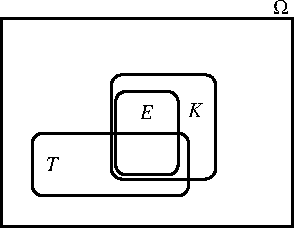
\includegraphics{images/ebola-1.pdf}
\caption{Ereignisse zum Experiment ``Person im Ebola-Gebiet''
\label{image-ebola}}
\end{figure}

In Abbildung~\ref{image-ebola} sind m"ogliche Ereignisse eines Experiments
dargestellt, bei dem ein zuf"allig ausgew"ahlte Person daraufhin untersucht
wurde, ob sie mit Ebola in Kontakt kam, daran erkrankte und inzwischen
verstorben ist.
Der einzelne Versuchsausgang ist also die Person, die f"ur die
Untersuchung ausgew"ahlt wurde.
Die Menge $\Omega$ ist die Menge aller Personen.
Folgende Ereignisse wurden untersucht:
\begin{align*}
K&=\{\omega\in\Omega\,|\,\text{$\omega$ ist mit Ebola in Kontakt gekommen}\}
\\
E&=\{\omega\in\Omega\,|\,\text{$\omega$ ist an Ebola erkrankt}\}
\\
T&=\{\omega\in\Omega\,|\,\text{$\omega$ ist verstorben}\}
\end{align*}
Es gilt nat"urlich $E\subset K$, denn wer an Ebola erkrankt, muss mit
Ebola in Kontakt gekommen sein.
Das umgekehrte gilt nicht, man kann durchaus mit Ebola in Kontakt
kommen, ohne daran zu erkranken.

Es gilt nicht, dass $E\subset T$, denn einerseits gibt es Personen, die
Ebola "uberlebt haben, und andererseits gibt es an Ebola erkrankte,
die zur Zeit des Experiments noch nicht verstorben sind.
Die Menge $E\cap T$ besteht aus denjenigen Personen, die an Ebola
erkrankt waren und verstorben sind.
Dies heisst aber nicht, dass sie an Ebola gestorben sind.
\end{beispiel}

Zwei Ereignisse $A$ und $B$ k"onnen bei der Durchf"uhrung des Experimentes
gleichzeitig eintreten.
Der Versuchsausgang $\omega$ ist also so beschaffen, dass mit ihm sowohl
$A$ als auch $B$ eintreten, dass also $\omega\in A$ und $\omega\in B$,
oder $\omega \in A\cap B$.
Gleichzeitiges Eintreten von Ereignis $A$ {\em und} $B$ ist das Ereignis
$A\cap B$.

Tritt ein Ereignis $A$ bei einer Versuchsdurchf"uhrung nicht ein, dann trat
ein Versuchsausgang $\omega$ auf, der nicht zu $A$ geh"ort,
also $\omega\in\Omega\setminus A$.
Dies bedeutet aber, dass das Ereignis $\Omega\setminus A=\overline{A}$
eingetreten ist.
Nichteintreten des Ereignisses $A$ ist das Ereignis
$\overline{A}=\Omega\setminus A$.

Zwei Ereignisse sind speziell.
Die Menge $\Omega\subset\Omega$ hat die Eigenschaft, dass jeder denkbare
Versuchsausgang per Definition in $\Omega$ liegt, das Ereignis $\Omega$
tritt also immer ein.
$\Omega$ heisst daher auch das sichere Ereignis.
\index{Ereignis!sicheres}
Die leere Menge $\emptyset\subset\Omega$ hat genau die gegenteilige
Eigenschaft: was auch immer geschieht, was auch immer f"ur ein 
Elementarereignis $\omega$ realisiert wird, in $\emptyset$ kann es
nicht drin sein, also wird $\emptyset$ nie eintreten.
$\emptyset$ heisst daher auch das unm"ogliche Ereignis.
\index{Ereignis!unm\"ogliches}

Diese Beispiele zeigen, dass die Modellierung von Ereignissen als Teilmengen
von $\Omega$
mit der umgangssprachlichen Sprechweise von Ereignissen "ubereinstimmt.
Die Tabelle~\ref{begriffe-zusammenfassung}
fasst die gebr"auchlichsten Mengenoperationen und die zugeh"orige
Sprechweise f"ur Ereignisse zusammen.

\begin{table}
\begin{center}
\begin{tabular}{|l|c|}
\hline
Begriff&Modell\\
\hline
Elementarereignis&$\omega$\\
alle Elementarereignisse&$\Omega$\\
Ereignis&$A\subset\Omega$\\
sicheres Ereignis&$\Omega$\\
unm"ogliches Ereignis&$\emptyset$\\
$A$ und $B$&$A\cap B$\\
$A$ oder $B$&$A\cup B$\\
$A$ hat $B$ zur Folge, $A\Rightarrow B$&$A\subset B$\\
nicht $A$&$\Omega\setminus A$\\
\hline
\end{tabular}
\end{center}
\caption{Begriffe der Wahrscheinlichkeitstheorie und ihre mathematischen
Modellierung\label{begriffe-zusammenfassung}}
\end{table}

\subsection{Beispiele}
\subsubsection{AIDS-Test}
Wenn sich jemand im Bezug auf AIDS riskant verhalten hat, dann ist
eine seiner Sorgen, dass der AIDS-Test nicht sofort das richtige
Resultat anzeigt.
Und selbst wenn er die notwendige Frist abgewartet
hat, hat der Test eine geringe Fehlerrate.
Es k"onnen also verschiedene Ereignisse eintreten.
Meistens wird ein
positiver AIDS-Test richtig anzeigen, dass eine Person HIV hat.
Manchmal
wird der Test jedoch positiv sein, obwohl die Person gesund ist
und manchmal wird der Test zwar ein negatives Resultat zeigen,
aber die Person ist an HIV erkrankt.
Gl"uck haben diejenigen, bei denen der Test nicht
anspricht, und die auch tats"achlich gesund sind.


\subsubsection{Euromillions}
\index{Euromillions}
\begin{figure}

\includegraphics[width=\hsize]{graphics/euromillions}
\caption{Besondere Gewinnchance bei Euromillions}
\end{figure}
\begin{figure}
\begin{center}
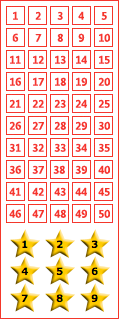
\includegraphics[height=8cm]{graphics/euromillionsschein}
\end{center}
\caption{Teilnahmeschein f"ur Euromillions\label{euromillionsschein}}
\end{figure}
Am 5.~September 2008 schrieb die Gratiszeitung ``20 Minuten'', dass die
bevorstehende Ziehung der Lotterie Euromillions besondere Gewinnchancen 
erm"ogliche, weil der Jackpot ungew"ohnlich gross sei.
Welche Ereignisse
sind in diesem Spiel relevant?

Auf der Euromillions-Website findet man die Erkl"arung, wie das Spiel abl"auft.
Der Spieler kreuzt auf dem Teilnahmeschein (Abbildung~\ref{euromillionsschein})
f"unf Zahlen und zwei Sterne an.
Dann erfolgt die Ziehung, Euromillions ermittelt
5 Gewinnzahlen aus dem Bereich 1--50 und 2 Gewinnsterne im Bereich 1--9.
Jetzt werden die "Ubereinstimmungen zwischen dem Tipp des Teilnehmers und den
Gewinnzahlen gez"ahlt.
Je besser die "Ubereinstimmung desto gr"osser der Gewinn.

\begin{table}
\begin{center}
\begin{tabular}{|c|c|c|c|}
\hline
Gewinnrang&richtige Zahlen&richtige Sterne&Anteil Gewinnsumme\\
\hline
1&5&2&32.0\%\\
2&5&1&7.4\%\\
3&5&0&2.1\%\\
4&4&2&1.5\%\\
5&4&1&1.0\%\\
6&4&0&0.7\%\\
7&3&2&1.0\%\\
8&3&1&5.1\%\\
9&2&2&4.4\%\\
10&2&0&4.7\%\\
11&1&2&10.1\%\\
12&2&1&24.0\%\\
\hline
\end{tabular}
\end{center}
\caption{Gewinnr"ange bei Euromillions\label{gewinnraenge}}
\end{table}

Die Tabelle \ref{gewinnraenge} zeigt, wie der Gewinn verteilt wird.
Offenbar spielen dabei sogenannte Gewinnr"ange eine besondere Rolle.
Bei jedem Tippzettel wird festgestellt, in welchen Gewinnrang er
geh"ort.

Ausser den Gewinnr"angen k"onnen auch andere Ereignisse eintreten,
die jedoch f"ur die Auszahlung nicht unbedingt von Bedeutung sind,
oder aus denen sich der Gewinn noch nicht ableiten l"asst:
\begin{itemize}
\item {\it Heiris Euromillions Teilnahmeschein f"allt in Gewinnrang 10.}
Offenbar teilt sich Heiri 4.7\% der Gewinnsumme mit den anderen Teilnehmern,
die dasselbe Ergebnis erzielt haben.
\item {\it Hanna hatte f"unf richtige Zahlen.}
Diese Information reicht noch nicht, um den Gewinn festzulegen.
Hannas Teilnahmeschein f"allt in Gewinnrang 1 oder 2 oder 3.
\item {\it Hermine hatte keinen einzigen Stern richtig.}
Hermine k"onnte
etwas gewonnen haben, n"amlich wenn sie 5, 4 oder 2 richtige Zahlen
gehabt hat (R"ange 3, 6 bzw.~10).
Oder sie k"onnte mit 3, 1 oder 0 richtigen Zahlen nichts gewonnen haben.
\item {\it Hermann hatte richtige Zahlen und Sterne.}
Hermann hatte als 1, 2, 3, 4 oder 5 richtige Zahlen {\em und}
1 oder 2 richtige Sterne.
\item {\it Es trifft nicht zu, dass Hilary einen richtigen Stern hat.}
\item {\it Holger hat auf 47 gesetzt.}
Dieses Ereignis nimmt auf die Ziehung "uberhaupt keinen Bezug,
trotzdem beschreibt es einen m"oglichen Ausgang des Experimentes.
\end{itemize}
Wir stellen fest, dass Ereignisse mit {\em und} (beide Ereignisse sind
eingetreten) und {\em oder} (eines der Ereignisse ist
eingetreten) verkn"upft werden k"onnen.
Ausserdem k"onnen Ereignisse negiert werden.

\subsection{Produkte}
\begin{figure}
\begin{center}
\begin{tabular}{|c|c|c|c|c|c|}
\hline
(1,1)&(1,2)&(1,3)&(1,4)&(1,5)&(1,6)\\
\hline
(2,1)&(2,2)&(2,3)&(2,4)&(2,5)&(2,6)\\
\hline
(3,1)&(3,2)&(3,3)&(3,4)&(3,5)&(3,6)\\
\hline
(4,1)&(4,2)&(4,3)&(4,4)&(4,5)&(4,6)\\
\hline
(5,1)&(5,2)&(5,3)&(5,4)&(5,5)&(5,6)\\
\hline
(6,1)&(6,2)&(6,3)&(6,4)&(6,5)&(6,6)\\
\hline
\end{tabular}
\end{center}
\caption{Elementarereignisse f"ur das W"urfeln mit zwei unterscheidbaren
W"urfeln\label{ereignisse-zwei-wuerfel}}
\end{figure}
Wir stellen uns vor, dass ein roter und ein blauer W"urfel geworfen werden.
Die von den beiden W"urfeln gezeigten Augenzahlen sind verschiedene
Versuchsausg"ange, sozusagen ``rote'' und ``blaue'' Zahlen.
Das Resultat
eines Wurfes ist also ein Paar bestehend aus einer ``roten'' und
einer ``blauen'' Augenzahl.
Die Menge aller m"oglichen Ausg"ange
ist also 
\[
\Omega = \Omega_{\text{rot}}\times\Omega_{\text{blau}},
\]
das kartesische Produkt der Mengen $\Omega_{\text{rot}}$ und
$\Omega_{\text{blau}}$ (siehe auch Abbildung \ref{ereignisse-zwei-wuerfel}).

In $\Omega$ lassen sich bereits bedeutend spannendere Ereignisse%
\footnote{\textit{Hinweis zu $A_2$}: $2|x \wedge 2|y$, sprich
	``2 teilt x und 2 teilt y'', ist "aquivalent:
	$x \equiv 0 \imod{2} \wedge y \equiv 0 \imod{2}$
} beschreiben:
\begin{align*}
A_1&=\{\text{mindestens eine ungerade Zahl}\}\\
   &=\{(x,y)\in\Omega\;|\;x \equiv 1 \imod{2} \vee y\equiv 1 \imod{2}\}\\
A_2&=\{\text{beide Augenzahlen sind gerade}\}\\
   &=\{(x,y)\in\Omega\;|\;2|x \wedge 2|y\}\\
X_i&=\{(i,y)\in\Omega\}\\
Y_i&=\{(x,i)\in\Omega\}\\
S_s&=\{(x,y)\in\Omega\;|\; x + y = s\}\\
D_d&=\{(x,y)\in\Omega\;|\; |x - y| = d\}\\
\end{align*}
Und damit lassen sich auch etwas spannendere Rechnungen durchf"uhren.
Zum Beispiel:
\begin{align*}
A_1&=\Omega \setminus A_2 = \bar A_2\\
A_1\cap A_2&=\emptyset\\
A_1&=X_1\cup X_3 \cup X_5\cup Y_1\cup Y_3\cup Y_5\\
X_4\cap Y_3&=\{(4,3)\}\\
X_5\cap S_7&=\{(5,2)\}\\
X_5\cap D_1&=\{(5,4), (5,6)\}\\
\end{align*}
\begin{figure}
\centering
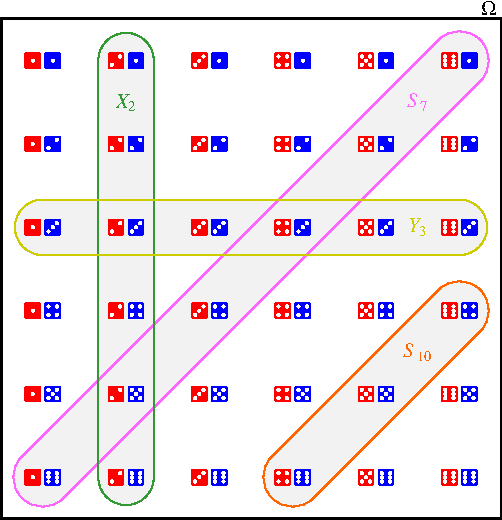
\includegraphics{images/zweiwuerfel-1.pdf}
\caption{Verschiedene Ereignisse in der Ereignisalgebra des Experiments
``Wurf zweier verschiedenfarbiger W"urfel\label{zweiwuerfel}''}
\end{figure}

\subsection{Formale Definition}
Damit obige Definition von Ereignissen funktioniert, m"ussen
alle Operationen in der Tabelle~\ref{begriffe-zusammenfassung}
ausf"uhrbar sein.
Die Menge aller Teilmengen von $\Omega$, die Potenzmenge
$P(\Omega)$ erf"ullt diese Bedingung,
ist aber sehr gross und hat sehr wenig n"utzliche Struktur, die
f"ur den Aufbau des Begriffs der Wahrscheinlichkeit im n"achsten
Abschnitt ben"otigt wird.
Insbesondere stellt sich heraus, dass es nicht m"oglich ist,
den Begriff der Wahrscheinlichkeit konsistent zu definieren, wenn
Ereignisse beliebige Teilmengen einer unendlichen Menge $\Omega$
sein d"urfen.

Ein Beispiel f"ur diese Situation sind Messwerte, in diesem
Fall ist $\Omega=\mathbb R$ unendlich.
Es werden aber auch nicht alle Teilmengen von $\mathbb R$ ben"otigt.
Es wird gen"ugen, wenn wir alle Intervalle zur Verf"ugung haben sowie
alle Mengen, die sich daraus durch endlich viele Mengenoperationen
konstruieren lassen.
Statt der Menge $P(\Omega)$ wird also eine kleinere Menge $\cal A$
von Ereignissen verwendet.
Man kann zeigen, dass sich aus der Menge der Intervalle immer 
eine Menge von Ereignissen konstruieren l"asst, in der alle
n"otigen Operationen ausgef"uhrt werden k"onnen, und auf der sich
die sp"ater einzuf"uhrende Wahrscheinlichkeit konsistent definieren
l"asst.

Die Einschr"ankung auf $\cal A$ hat mindestens im Rahmen dieser
Vorlesung keine praktischen Konsequenzen, alle interessierenden
Ereignisse sind von vornherein in $\cal A$, und damit auch alle daraus
abgeleiteten Ereignisse.

Wir nennen eine solche Menge von Ereignissen eine Ereignisalgebra:

\begin{definition}
\label{def-ereignisalgebra}
Eine {\em Ereignisalgebra} $(\Omega,{\cal A})$ ist
eine Menge $\Omega$ mit einer Menge ${\cal A }\subset{\cal P}(\Omega)$
von Teilmengen von $\Omega$, die folgende Bedingungen erf"ullen:
\begin{enumerate}
\item Vereinigungen von Elementen von ${\cal A}$ sind ebenfalls in ${\cal A}$,
also
\[
A,B\in {\cal A}\Rightarrow A\cup B\in{\cal A}
\]
\item Differenzen von Elementen von ${\cal A}$ sind in ${\cal A}$, also
\[
A,B\in {\cal A}\Rightarrow A\setminus B\in{\cal A}
\]
\item $\Omega\in{\cal A}$, d.~h.~es gibt das sichere Ereignis.
\end{enumerate}
\end{definition}

Sind nur die Bedingungen 1 und 2 erf"ullt, spricht man auch von einem
Mengen-Ring.
Eine Ereignisalgebra heisst manchmal auch ein Mengenk"orper.

Aus den Axiomen f"ur die Ereignisalgebra lassen sich sofort erste
Schlussfolgerungen ziehen:
\begin{enumerate}
\item Es gibt auch das unm"ogliche Ereignis: $\emptyset = \Omega\setminus\Omega\in{\cal A}$.
\item Das Komplement eines Ereignisses ist ebenfalls ein Ereignis: $\bar A=\Omega\setminus A\in{\cal A}$.
\item Der Durchschnitt zweier Ereignisse ist ebenfalls ein Ereignis: $A\cap B = 
(A\cup B) \setminus ((A\setminus B) \cup (B\setminus A))\in{\cal A}$.
\end{enumerate}

\section{Weitere Beispiele von Ereignisalgebren} \label{section-beispiele}
\subsection{Dominosteine}
Die Menge aller m"oglichen Dominosteine wurde bereits fr"uher untersucht.
Jetzt m"ochten wir darin einzelne Ereignisse auszeichnen.
Wir beschreiben
einen einzelnen Dominostein als ein paar $(x,y)$, wobei $x\ge y$ sein soll.
Beispiele von Ereignissen:
\begin{align*}
S_k&=\{ \text{Die Augensumme ist $k$}\}\\
S_5&=\{ (5,0), (4,1), (3,2) \}\\
S_4&=\{ (4,0), (3,1), (2,2) \}\\
R&=\{\text{die Augenzahlen sind positiv haben keinen gemeinsamen Teiler $>1$}\}\\
 &=\{ (6,5), (6,1), (5,4), (5,3), (5,2), (5,1), (4,3), (4,1), (3,2), (3,1), (2,1), (1,1) \}
\\
P&=\{\text{beide Augenzahlen sind Primzahlen}\}\\
 &=\{(5,5), (5,3), (5,2), (3,3), (3,2), (2,2) \}\\
\end{align*}

\subsection{W"urfeln mit zwei W"urfeln}
Bei einem W"urfelspiel wirft man jeweils zwei W"urfel.
Zeigen beide W"urfel
die gleiche Zahl, man nennt dies einen {\em Pasch}, darf man genau ein
weiteres Mal w"urfeln.
Die Elementarereignisse sind also entweder einfach Paare, also von
der Form $(x,y)$, mit $x\ne y$, oder ein Pasch gefolgt von irgend einem
W"urfelresultat, wir schreiben dies $(P_k, (x,y))$, also ein $k$-er-Pasch
gefolgt von einem Paar $(x,y)$, wobei diesmal keine Einschr"ankungen f"ur
$x$ und $y$ gelten.
Damit kann man jetzt alle m"oglichen Elementarereignisse auflisten
\begin{align*}
\Omega=\{
&\phantom{(6,6),} (6,5), (6,4), (6,3), (6,2), (6,1)\\
&(5,6), \phantom{(5,5),} (5,4), (5,3), (5,2), (5,1)\\
&(4,6), (4,5), \phantom{(4,4),} (4,3), (4,2), (4,1)\\
&(3,6), (3,5), (3,4), \phantom{(3,3),} (3,2), (3,1)\\
&(2,6), (2,5), (2,4), (2,3), \phantom{(2,2),} (2,1)\\
&(1,6), (1,5), (1,4), (1,3), (1,2), \phantom{(1,1)}
\}
\\
&\cup
\{(P_6,(x,y))\}
\cup
\{(P_5,(x,y))\}
\cup
\{(P_4,(x,y))\}
\\
&\cup
\{(P_3,(x,y))\}
\cup
\{(P_2,(x,y))\}
\cup
\{(P_1,(x,y))\}
\end{align*}
Man sieht daraus zum Beispiel, dass es $30 + 6\cdot 36=246$
Elementarereignisse gibt.
Darin enthalten sind die Ereignisse
\begin{align*}
P&=\{\text{Pasch im ersten Wurf}\}\\
&=
\{(P_6,(x,y))\}
\cup
\{(P_5,(x,y))\}
\cup
\{(P_4,(x,y))\}
\\
&\qquad \cup
\{(P_3,(x,y))\}
\cup
\{(P_2,(x,y))\}
\cup
\{(P_1,(x,y))\}
\\
\tilde P_k&=\{\text{$k$-er Pasch im ersten Wurf}\}\\
   &=\{(P_k,(x,y))\}
\\
Q&=\{\text{totale Augensumme $\ge 10$}\}\\
&=\{\phantom{(6,6),} (6,5), (6,4), \\
&\phantom{\;=\{}(5,6), \phantom{(5,5), (5,4)} \\
&\phantom{\;=\{}(4,6)\phantom{, (4,5), (4,4)}
\}
\\
&\qquad\cup
\{(P_6,(x,y))\}
\cup
\{(P_5,(x,y))\}
\cup
\{(P_4,(x,y))\,|\, x+y \ge 2\}
\\
&\qquad\cup
\{(P_3,(x,y))\,|\, x+y \ge 4\}
\cup
\{(P_2,(x,y))\,|\, x+y \ge 6\}
\\
&\qquad
\cup
\{(P_1,(x,y))\,|\, x+y \ge 8\}
\end{align*}

\subsection{AIDS-Test}
Wir mathematisieren das Beispiel des AIDS-Tests.
Die fr"uhere Diskussion f"uhrt uns vor Augen,
dass wir hier mit zwei verschiedenen Ereignissen zu tun haben. 
Das Experiment besteht offenbar darin, dass wir jemanden untersuchen,
die Menge der Elementarereignisse ist also die Menge aller betrachteten
Personen.
Darin unterscheiden wir:
\begin{align*}
H&=\{\text{Person hat HIV}\}\\
T&=\{\text{Person hat positiven AIDS-Test}\}
\end{align*}
Es ist klar, dass $H\ne T$.
Es gibt Personen, die zwar HIV haben, bei
denen der Test dies aber noch nicht zeigen kann, $H\setminus T\ne \emptyset$.
Andererseits gibt es falsche positive Testresultate,
$T\setminus H\ne\emptyset$. 

\subsection{Messwertalgebra}
\begin{table}
\begin{center}
\begin{tabular}{|cc|cc|}
\hline
1&0.990
&11&0.990\\
2&0.989
&12&0.989\\
3&0.991
&13&0.990\\
4&0.991
&14&0.991\\
5&0.991
&15&0.989\\
6&0.989
&16&0.990\\
7&0.990
&17&0.989\\
8&0.989
&18&0.990\\
9&0.992
&19&0.990\\
10&0.992
&20&0.991\\
\hline
\end{tabular}
\end{center}
\caption{Werte von Stichprobe von 20 1k$\Omega$-Widerst"anden\label{widerstandswerte}}
\end{table}
Bei einer Messung wird ein Messwert ermittelt, dieser kann jedoch
nur mit einer begrenzten Genauigkeit festgehalten werden.
Die Elementarereignisse sind zwar immer noch alle m"oglichen reellen
Zahlen $\mathbb R$, aber sinnvolle Ereignisse sind nur bestimmte Teilmengen
$A\subset\mathbb R$.
Wir wollen bestimmen, welche Teilmengen das sind.

Zun"achst f"uhren wir dies an einem Beispiel durch.
Bei einer am 1.~November 2006
zuf"allig bei Pusterla in Z"urich gekauften Stichprobe von 20 1k$\Omega$
Widerst"anden ergaben sich beim Nachmessen die Widerstandswerte in 
Tabelle \ref{widerstandswerte}.
Offensichtlich streuen die Messwerte
zwischen 0.989 und 0.992.
Genauere Informationen kann das Messger"at nicht
anzeigen.
Wir k"onnen aus den Daten also eigentlich nur folgendes schliessen:
der Widerstand mit der Nummer eins hat einen Wert $0.990\le R_1<0.991$.
Der Widerstandswert $R_1$ ist ein Versuchsergebnis, also ein Elementarereignis,
liegt aber in der Menge
\[
A=[0.990,0.991)\subset \mathbb{R}=\Omega.
\]
Ausserdem werden durch die weiteren Messungen auch noch folgende
Ereignisse realisiert:
\begin{center}
\begin{tabular}{|c|c|}
\hline
Ereignis&H"aufigkeit\\
\hline
$[0.989,0.990)$&6\\
$[0.990,0.991)$&7\\
$[0.991,0.992)$&5\\
$[0.992,0.993)$&2\\
\hline
\end{tabular}
\end{center}
Diese speziellen Ereignisse beinhalten offensichtlich alle Information,
die wir "uber die Widerst"ande haben k"onnen.
Bei den 20 Versuchen treten aber auch noch andere Ereignisse ein,
zum Beispiel
\begin{center}
\begin{tabular}{|c|c|}
\hline
Ereignis&H"aufigkeit\\
\hline
$\{R\ge 0.990\}$&14\\
``5\% Toleranz'' = $\{0.95\le R\le1.05\}$&20\\
``1\% Toleranz'' = $\{0.99\le R\le 1.01\}$&14\\
\hline
\end{tabular}
\end{center}

Etwas formaler: Eine Genauigkeitsangabe bei einem Messwert definiert
ein Intervall, in dem sich ein Messwert befinden muss.
Wir
fordern also, dass $\cal A$ alle Intervalle der Form $[a,b]\subset\mathbb R$
enthalten muss.
Aber auch die Aussage ``der Messwert ist kleiner als $a$''
muss einem Ereignis in $\cal A$ entsprechen, also m"ussen auch Intervalle,
die sich ins unendliche erstrecken in $\cal A$ sein:
\begin{align*}{}
(-\infty,r]&=\{x\in\mathbb R\;|\;x \le r\} \in \cal A\\
% Hack: \; brauchts, damit eqnarray nicht meint [ leite ein Argument ein
\;[r,\infty)&=\{x\in\mathbb R\;|\;x \ge r\} \in \cal A
\end{align*}

Da wir Komplemente bilden k"onnen, m"ussen auch die offenen Intervalle
\begin{align*}
\overline{[a,\infty)}&=\mathbb R\setminus [a,\infty)=(-\infty,a)\in\cal A\\
\overline{(-\infty,b]}&=\mathbb R\setminus (-\infty,b]= (b,\infty)\in\cal A
\end{align*}
Ereignisse sein.
Ein beliebiges offenes Intervall l"asst sich
als Durchschnitt zweier solcher Intervalle ausdr"ucken:
\[
(a,b)=(-\infty, b)\cap(a,\infty).
\]
Durch Bildung von geeigneten Durchschnitten lassen sich also alle
Intervalle bilden.
Ausserdem m"ussen alle Teilmengen von $\mathbb R$
zu $\cal A$ hinzugenommen werden, die sich durch Bildung von Komplementen,
Durchschnitten und Vereinigungen bilden lassen.
Offensichtlich ist $\cal A$
in diesem Falle sehr kompliziert.

\section{Wahrscheinlichkeit} \label{section-wahrscheinlichkeit}
In der Einleitung haben wir das Ereignis diskutiert, dass die Schweizer
Nati ein bestimmtes Spiel an Fussball WM gewinnt.
Wir sind zum Schluss
gekommen dass wir nicht wissen k"onnen, was bei der konkreten
Durchf"uhrung des Experimentes passieren wird.
Falls der Gegner
stark ist, zum Beispiel Deutschland, dann wird ein Sieg wohl auch
dann kaum je eintreten, wenn man das Spiel viele Male wiederholt.
Das wenigstens verbinden wir mit einem unwahrscheinlichen Ereignis.
Trotzdem kann das Ereignis eintreten.

\subsection{Verschiedene Wahrscheinlichkeitsbegriffe}
Die Wahrscheinlichkeit soll ein Mass daf"ur sein, dass ein Ereignis
eintritt.
Es gibt verschiedene Ans"atze, wie wir zu einem solchen Mass kommen
k"onnten:
\begin{itemize}
\item 
Je h"aufiger ein Ereignis eintritt, desto gr"osser sollte die
Wahrscheinlichkeit sein.
Dies setzt voraus, dass das Experiment im Prinzip beliebig oft wiederholbar 
ist.
Man nennt dies den {\em frequentistischen} Ansatz.
\item
Die Wahrscheinlichkeit ist ein Mass f"ur die pers"onliche
"Uberzeugung, dass ein Ereignis eintreten wird.
Im Unterschied zum frequentistischen Ansatz sollte man bei diesem
Ansatz einem Ereignis auch dann eine Wahrscheinlichkeit geben k"onnen,
wenn sich ein Experiment nicht wirklich wiederholen l"asst.
Dies ist der Bayessche Ansatz.
\item
Wir k"onnten eine Reihe von Axiomen postulieren, nach denen sich
die Wahrscheinlichkeit zu verhalten hat, und dann zu untersuchen,
ob ein solches Objekt tats"achlich existiert.
\end{itemize}
In allen F"allen ergibt sich eine Reihe von Gesetzm"assigkeiten
oder Formeln, welche die jeweiligen Wahrscheinlichkeitsbegriffe 
erf"ullen m"ussen.
Soll die Wahrscheinlichkeit eine objektive Gr"osse sein, dann
muss f"ur wiederholbare Experimente die f"ur den Bayesschen
Ansatz n"otige pers"onliche "Uberzeugung direkt mit der H"aufigkeit
des Eintretens zusammenh"angen.
Der frequentistische und der Bayessche Ansatz werden also in diesem
Fall "ubereinstimmen.
Die Axiome im axiomatischen Ansatz sind nat"urlich genau die
Rechenregeln, die man sowohl im frequentistischen Ansatz wie
auch im Bayesschen Ansatz von der Wahrscheinlichkeit erwartet.
Man darf daher davon ausgehen, dass die drei Ans"atze die gleichen numerischen
Resultate liefern, sie unterscheiden sich h"ochstens in der Interpretation
der Resultate.
Wir werden daher im Folgenden vor allem den am leichtesten zu
verstehenden frequentistischen Ansatz verfolgen.

\subsection{Wahrscheinlichkeit als relative H"aufigkeit}
Wir wollen nun einen Begriff der Wahrscheinlichkeit einf"uhren, der
einer intuitiven Vorstellung zu diesem Wort m"oglichst nahe kommt.
Wenn ``sehr
wahrscheinlich'' heissen soll ``in der Mehrzahl der F"alle'', dann
bedeutet das offensichtlich, dass man eine gr"ossere Zahl von
Experimenten durchf"uhren soll, und dann die F"alle z"ahlen soll,
in denen das Ereignis tats"achlich eingetreten ist.
Deren Anteil
an der Gesamtzahl heisst {\em relative H"aufigkeit} und ist eine erste,
etwas pr"azisere Fassung des Begriffs der Wahrscheinlichkeit.

Grundlegend f"ur die Wahrscheinlichkeitsrechnung ist die aus der
\index{Wahrscheinlichkeit!als relative H\"aufigkeit}
Erfahrung mit einer grossen Zahl von Versuchen gewonnene Zuversicht,
dass die relative H"aufigkeit mit wachsender Anzahl Versuche gegen
eine Gr"osse $P(A)$ strebt.
Man verwendet diese Annahme daher als Definition.
Wiederholt man ein Experiment $N$ Male, und tritt dabei das Ereignis $A$
genau $n$ mal ein, dann erwartete man, dass der Quotient $\frac{n}{N}$
eine gute N"aherung f"ur $P(A)$ ist.
Je "ofter man das Experiment
wiederholt, desto n"aher sollte der Quotient der Gr"osse $P(A)$
kommen, also
\[
P(A) := \lim_{N\to\infty}\frac{n}{N}.
\]

Leider ist es nur selten praktikabel, das Experiment tats"achlich
sehr h"aufig zu wiederholen.
Bei der Pr"ufung neuer Medikamente
zum Beispiel hindern moralische Bedenken daran, eine grosse
Zahl von Experimenten mit Menschen durchzuf"uhren.
Bei der
Ausbruchswahrscheinlichkeit eines Vulkans oder der
Einschlagwahrscheinlichkeit eines Asteroiden auf der Erde hat man
ganz einfach keine Kontrolle "uber das Experiment.

Das Ziel der Wahrscheinlichkeitstheorie ist daher, 
die Abbildung $P\colon {\cal A}\to\mathbb{R}$
abstrakt zu definieren und geeignete Axiome zu postulieren, die
der eben skizzierten intuitiven Vorstellung der Wahrscheinlichkeit
einen strengen Sinn geben.
Damit wird die Funktion $P$ in vielen
F"allen berechenbar, meist nat"urlich unter zus"atzlichen Annahmen.
Die grundlegenden Eigenschaften sind in den folgenden, f"ur
relative H"aufigkeiten, unmittelbar einleuchtenden Axiomen
% XXX
von Kolmogorov\footnote{Andrei Nikolaiewitsch Kolmogorov, 1903-1987}
festgehalten.
\index{Kolmogorov, Andrei Nikolaiewitsch}

\subsubsection{Axiome  eines Wahrscheinlichkeitsraumes}
\index{Axiome eines Wahrscheinlichkeitsraumes}

\begin{description}
\item[Wertebereich.]F"ur jedes beliebige Ereignis $A\subset \Omega$
gilt
\begin{equation}
0\le P(A)\le 1.
\label{p-wertebereich}
\end{equation}
\item[Sicheres Ereignis.] F"ur das sichere Ereignis gilt
\begin{equation}
P(\Omega) = 1.
\label{p-sicheresereignis}
\end{equation}
\item[Vereinigung.] Sind die Ereignisse $A_1,A_2,\dots$ paarweise
disjunkt, also $A_i\cap A_j=\emptyset$ f"ur $i\ne j$, dann gilt
\begin{equation}
P(A_1\cup A_2\cup \dots) = P(A_1) + P(A_2) + \dots
\label{p-summenformel}
\end{equation}
\end{description}

Die Forderung "uber die Vereinigung kann nat"urlich nur dann "uberhaupt
formuliert werden, wenn die Vereinigung auch wirklich ein Ereignis ist, also in
$\cal A$ ist.
Bisher wissen wir nur, dass endliche
Vereinigungen von Ereignissen gebildet werden k"onnen, jetzt m"ussen
wir fordern, dass
auch unendliche Vereinigungen von Ereignissen wieder Ereignisse sind.
D.~h.~wir setzen im Folgenden voraus, dass in einer
Ereignisalgebra in Erweiterung des ersten Axioms auch gilt:

\begin{definition}
$\cal A$ heisst 
$\sigma$-Algebra, wenn 
abz"ahlbare Vereinigungen von Elementen von $\cal A$ ebenfalls
in $\cal A$ sind, d.~h.~falls $A_i\in{\cal A}$ f"ur $i\in\mathbb{N}$, dann ist
\[
A_1\cup A_2\cup\dots=\bigcup_{i=0}^{\infty}A_i \in{\cal A}.
\]
\end{definition}

In allen praktischen F"allen ist diese technische Bedingung automatisch
erf"ullt, oder man kann erzwingen, dass sie erf"ullt ist.
F"ur die Praxis ist dies also keine Einschr"ankung, man kann immer davon
ausgehen, dass die Vereinigungsformel~(\ref{p-summenformel}) ``funktioniert''.

\subsection{Beispiel: W"urfeln}
Beim W"urfeln mit einem W"urfel erwartet man, dass jeder m"ogliche
Ausgang etwa gleich h"aufig sein wird.
Bei einer grossen Zahl von
Versuchen wird man also feststellen, dass die relative H"aufigkeit
des Ereignisses, dass eine $4$ gew"urfelt wird, gegen $\frac16$
konvergieren wird.
Die zus"atzliche Annahme steckt in diesem Fall
darin, dass man alle Ausg"ange als gleich wahrscheinlich annimmt.

\begin{table}
\begin{center}
\begin{tabular}{|l|r|r|r|r|r|r|r|r|}
\hline
Anzahl&6&96&996&9996&99996&999996&9999996&99999996\\
\hline
0& 0& 17& 168& 1642& 16746& 166434& 1665609& 16662248\\
1& 1& 17& 160& 1692& 16747& 166584& 1666841& 16669513\\
2& 1& 11& 178& 1680& 16491& 167031& 1667271& 16663991\\
3& 0& 16& 158& 1660& 16672& 165940& 1665310& 16659406\\
4& 3& 13& 159& 1634& 16756& 167026& 1668244& 16672749\\
5& 1& 22& 173& 1688& 16584& 166981& 1666721& 16672089\\
\hline
Maximum& 3& 22& 178& 1692& 16756& 167031& 1668244& 16672749\\
Minimum& 0& 11& 158& 1634& 16491& 165940& 1665310& 16659406\\
$\Delta$& 3& 11& 20& 58& 265& 1091& 2934& 13343\\
\hline
\end{tabular}
\end{center}
\caption{Computer-Simulation eines fairen W"urfels\label{wuerfel-simulation}}
\end{table}

Die tats"achliche Durchf"uhrung von ``gen"ugend'' vielen Experimenten
kann hingegen schwierig sein.
Eine Computer-Simulation des
W"urfel-Experiments zeigt zum Beispiel die Resultate in Tabelle
\ref{wuerfel-simulation}.
Offensichtlich ist selbst mit $10^8$
W"urfen die Wahrscheinlichkeit erst auf drei Stellen nach dem Komma
genau.

\subsection{Folgerungen aus den Axiomen}
\begin{satz}Es gilt
\begin{enumerate}
\item Die Wahrscheinlichkeit des unm"oglichen Ereignisses ist
\begin{equation}
P(\emptyset) = 0.
\label{p-emptyset}
\end{equation}
\item Die Wahrscheinlichkeit des komplement"aren Ereignisses
ist
\begin{equation}
P(\bar A) = P(\Omega\setminus A) = 1 -P(A).
\label{p-negation}
\end{equation}
\item Die Wahrscheinlichkeit der Differenz der Ereignisse $A$ und $B$
ist
\begin{equation}
P(A\setminus B) = P(A) - P(A\cap B)
\label{p-complement} % changed
\end{equation}
\item Die Wahrscheinlichkeit der Vereinigung zweier beliebiger Ereignisse
ist
\begin{equation}
P(A\cup B) = P(A) + P(B) - P(A\cap B)
\label{p-union}
\end{equation}
(Ein-/Ausschaltformel).
\index{Ein-/Ausschaltformel}
\end{enumerate}
\end{satz}

\begin{proof}[Beweis]
Wegen $\Omega = \Omega \cup\emptyset$ und
$\Omega\cap\emptyset = \emptyset$ folgt aus dem Axiom
"uber die Vereinigung  (\ref{p-summenformel})
\[
P(\Omega) = P(\Omega \cup \emptyset) = P(\Omega) + P(\emptyset)
\]
Indem man auf beiden Seiten der Gleichung $P(\Omega)$ subtrahiert,
folgt $0 = P(\emptyset)$.

F"ur das komplement"are Ereignis gilt $A\cap\bar A=\emptyset$ und
$A\cup\bar A=\Omega$.
Aus der Summenformel (\ref{p-summenformel}) folgt
\[
1 = P(\Omega) = P(A\cup\bar A) = P(A) + P(\bar A)
\]
oder
\[
P(\bar A) = 1 - P(A).
\]

$A$ ist die disjunkte Vereinigung $A=(A\setminus B) \cup (A\cap B)$,
also gilt
\[
P(A)=P(A\setminus B) + P(A\cap B),
\]
oder, nach $P(A\setminus B)$ aufgel"ost
\[
P(A\setminus B) = P(A) - P(A\cap B).
\]

Nach der de Morganschen Regel l"asst sich die Vereinigungsmenge
als disjunkte Vereinigung schreiben:
\[
A\cup B =  (A\setminus B) \cup (A\cap B) \cup (B\setminus A)
\]
Also gilt
\begin{align*}
P(A\cup B)&=P(A\setminus B) + P(A\cap B) + P(B\setminus A)\\
&=P(A) - P(A\cap B) + P(A\cap B) + P(B) - P(A\cap B)\\
&=P(A) + P(B) - P(A\cap B).
\end{align*}
\end{proof}
Damit stehen uns Rechenregeln zur Verf"ugung, mit deren Hilfe wir
die Wahrscheinlichkeit beliebiger Ereignisse auf der Basis einiger
weniger Annahmen berechnen k"onnen.

\subsection{Wahrscheinlichkeit als Mass}
Die Wahrscheinlichkeitsfunktion $P$ hat genau die Eigenschaften,
die man von einer Fl"achenmessung erwartet.
Die Gesamtfl"ache disjunkter Fl"achenst"ucke berechnet man,
indem man den Fl"acheninhalt der einzelnen Fl"achenst"ucke summiert.
Das leere Fl"achenst"uck hat keinen Inhalt.
Einzig die zus"atzliche Forderung $P(\Omega)=1$, welche
sicherstellt, dass die Wahrscheinlichkeit nicht gross werden kann,
hat keine Entsprechung.

Demzufolge k"onnen Ereignisse oft auch als Fl"achen in einem Diagramm
visualisiert werden,
die umso gr"osser sind, je gr"osser die Wahrscheinlichkeit des Ereignisses
ist.
Bei einem Dart-Spiel liegt es nahe, dass die Wahrscheinlichkeit, ein
bestimmtes Feld zu treffen, umso gr"osser ist, je gr"osser der Fl"achen-Anteil
dieses Feldes an der ganzen Scheibe ist.
Nat"urlich trifft dies nur bei einem
sehr schlechten Dart-Spieler zu, dessen Pfeile gleichm"assig verteilt auf
die Scheibe treffen.

Diese
"Uberlegung kann jedoch dazu verwendet werden, die Wahrscheinlichkeiten
eines Meteoriteneinschlages in der Schweiz und im F"urstentum Liechtenstein
miteinander zu vergleichen.
Wir erwarten, dass die Wahrscheinlichkeit
proportional zur Fl"ache sein wird, also
\[
\frac{P(\text{CH})}{P(\text{FL})}=
\frac{41285\text{km$\mathstrut^2$}}{160\text{km$\mathstrut^2$}}
=258.03,
\]
die Wahrscheinlichkeit f"ur einen Meteoriteneinschlag im L"andle ist also
"uber 258mal kleiner.

Umgekehrt k"onnte man die Idee zu einer Fl"achenberechnungs- oder
Integra\-tions\-methode ausbauen.
Um den Fl"acheninhalt einer unregelm"assigen
Teilmenge
eines Rechteckes in der Ebene zu bestimmen, simuliert man mit dem
Computer gleichm"assig verteilte ``Sch"usse'' auf diese ``Zielscheibe''.
Der Anteil der Treffer in der Teilmenge ergibt ein Mass f"ur dessen
Fl"ache.
Leider ist das Verfahren in dieser Form praktisch nicht
durchf"uhrbar, weil viel zu viele ``Sch"usse'' notwendig sind, um
eine gen"ugende Genauigkeit zu erreichen.
Es kann aber durchaus
zu einem praktikablen Verfahren verfeinert werden (Monte Carlo Methoden).

Wegen
der Analogie zu einer Fl"achenmessung heisst eine
Wahrscheinlichkeitsfunktion $P$ oft auch ein {\em Wahrscheinlichkeitsmass}.
Das Tripel $(\Omega,{\cal A}, P)$ heisst ein {\em Wahrscheinlichkeitsraum}.

\section{Laplace-Experimente} \label{section-laplace-ereignisse}
Bisher sind wir nicht in der Lage, die Wahrscheinlichkeit eines Ereignisses
zu berechnen, wir k"onnen nur mit Hilfe der Axiome aus bereits bekannten
Wahrscheinlichkeiten neue Wahrscheinlichkeiten berechnen.
F"ur die Berechnung der Wahrscheinlichkeiten ist zus"atzliche
Information n"otig.

Bei Experimenten mit endlich vielen Ausg"angen ist es manchmal gerechtfertigt
anzunehmen, dass alle Versuchsausg"ange gleich h"aufig und damit gleich
wahrscheinlich sind.
Von einem guten W"urfel erwarten wir, dass er alle Seiten gleich h"aufig
zeigt, eine symmetrische M"unze sollte Kopf und Zahl etwa gleich h"aufig
zeigen.
Unter dieser Annahme k"onnen wir die Wahrscheinlichkeit berechnen:

\begin{definition}
Ein Experiment mit $n=|\Omega|$ Ausg"angen heisst ein {\em Laplace-Experiment},
wenn jeder Versuchsausgang gleich wahrscheinlich mit Wahrscheinlichkeit
\[
P(\{\omega\})=\frac1n,\qquad\omega\in\Omega
\]
ist.
\end{definition}

Da Laplace-Experimente nur endliche viele Ausg"ange haben, kann man aus
den Axiomen auch jede andere Wahrscheinlichkeit berechnen:

\begin{satz}
Bei einem Laplace-Experiment tritt das Ereignis $A\subset\Omega$ mit
Wahrscheinlichkeit
\[
P(A)=\frac{|A|}{|\Omega|}
\]
ein.
\end{satz}
Damit ist die Berechnung der Wahrscheinlichkeit auf das Z"ahlen der 
Versuchsausg"ange in $A$ reduziert, also auf eine Kombinatorik-Aufgabe.

\subsection{M"unze werfen}
\index{Munze@{M\"unze, faire}}
Wirft man eine M"unze, kann sie nur auf einer von zwei Seiten landen,
die Elementarereignisse sind also $\Omega = \{\text{Kopf}, \text{Zahl}\}$.
Die mathematisch idealisierte M"unze ist so d"unn, dass sie nicht auf
der Kante stehen kann.
Nach allgemeiner Erfahrung funktioniert f"ur
solche M"unzen der Ansatz von Laplace, d.~h.~$P(\text{Kopf}) = \frac12$
und $P(\text{Zahl})=\frac12$.

Selbstverst"andlich gibt es auch M"unzen, f"ur die die Laplace-Annahme
nicht funktioniert, gebogene M"unzen fallen zum Beispiel bevorzugt auf die
nach aussen gew"olbte Fl"ache.

\subsection{W"urfeln}
\index{Wurfel@{W\"urfel, fairer}}
W"urfel haben sechs Seiten, die gem"ass der Annahme eines Laplace-Experiments
mit gleicher
Wahrscheinlichkeit oben liegen werden, die Wahrscheinlichkeit jedes
Resultates ist also gleich $P(i) = \frac16, i\in\{1,2,3,4,5,6\}$.
Wird eine Seite des W"urfels beschwert, f"allt er bevorzugt auf diese
Seite, und die Wahrscheinlichkeiten sind nicht mehr gleich.

\begin{figure}
\begin{center}
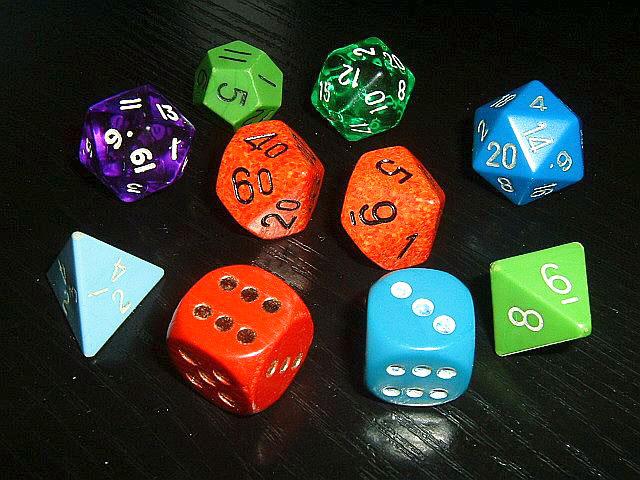
\includegraphics[width=0.8\hsize]{graphics/Wuerfel5}
\end{center}
\caption{Verschiedene Spielw"urfel\label{bild-spielwuerfel}}
\end{figure}
Man kann auch aus anderen geometrischen K"orpern ``W"urfel'' bauen, die
eine gr"ossere Zahl von Ausg"angen erm"oglichen.
Ein Dodekaeder hat
zw"olf Seiten, ein Ikosaeder sogar deren 20, aber auch andere Formen
sind realisierbar, siehe Abbildung~\ref{bild-spielwuerfel}.
Der Einfachheit
halber gehen wir im Folgenden immer von sechsseitigen W"urfeln aus.

Das Werfen eines solchen W"urfels erzeugt die folgenden Elementarereignisse
oder Versuchsergebnisse:
\[
\Omega=\{1,2,3,4,5,6\}.
\]
Nach dem Laplace'schen Ansatz wird jedem Elementarereignis die
Wahrscheinlichkeit $\frac16$ zugeschrieben.
Damit lassen sich
Wahrscheinlichkeiten berechnen:
\begin{align*}
P(\text{``gerade Zahl''})=P(\{2,4,6\})&=\frac36=0.5\\
P(\text{``durch 3 teilbar''})=P(\{3,6\})&=\frac26=0.333\\
P(< 7)=P(\Omega)&=\frac66=1
\end{align*}

\subsection{Zwei W"urfel}
In verschiedenen Spielen wird mit zwei W"urfeln gespielt, wobei nur
deren Augensumme interessiert.
Die Ereignisalgebra dazu wurde bereits
fr"uher vorgestellt, die Elementarereignisse sind Paare $(i,j)$ aus
den Augenzahlen der beiden W"urfel.
Die Menge der Elementarereignisse
ist also
% hier brauchen wir wirklich ein eqnarray, wegen dem Spacing
\begin{eqnarray*}
\Omega=&\{&\\
&&(1,1),(1,2),(1,3),(1,4),(1,5),(1,6),\\
&&(2,1),(2,2),(2,3),(2,4),(2,5),(2,6),\\
&&(3,1),(3,2),(3,3),(3,4),(3,5),(3,6),\\
&&(4,1),(4,2),(4,3),(4,4),(4,5),(4,6),\\
&&(5,1),(5,2),(5,3),(5,4),(5,5),(5,6),\\
&&(6,1),(6,2),(6,3),(6,4),(6,5),(6,6),\\
&\},&
\end{eqnarray*}
und $|\Omega|=36$.
Wenn nur die Augensumme interessiert, dann will
man offensichtlich die Ereignisse
\begin{align*}
A_2&=\{\Sigma=2\}=\{(1,1)\}\\
A_3&=\{\Sigma=3\}=\{(1,2),(2,1)\}\\
A_4&=\{\Sigma=4\}=\{(1,3),(2,2),(3,1)\}\\
&\vdots\\
A_{12}&=\{\Sigma=12\}=\{(6,6)\}
\end{align*}
untersuchen.
Diese Ereignisse sind einfach auszuz"ahlen, und damit kann man auch
die Wahrscheinlichkeiten bestimmen:
\begin{align*}
P(A_2)=P(A_{12})&=\frac{1}{36},\\
P(A_3)=P(A_{11})&=\frac{2}{36},\\
P(A_4)=P(A_{11})&=\frac{3}{36},\\
P(A_5)=P(A_9)&=\frac{4}{36},\\
P(A_6)=P(A_8)&=\frac{5}{36},\\
P(A_7)&=\frac{7}{36}.
\end{align*}

\subsection{Geburtstagsproblem}
Wie gross ist die Wahrscheinlichkeit, dass unter $n$ Personen zwei
am gleichen Tag Geburtstag haben? Hierbei nimmt man an, dass
jeder Tag im Jahr etwa gleich h"aufig als Geburtstag
vorkommt\footnote{Dies ist
jedoch nicht ganz richtig, wie Geb"arabteilungen in Spit"alern
best"atigen k"onnen.
Auch haben gr"ossere Stromausf"alle h"aufig
einen Geburtenzuwachs ungef"ahr neun Monate sp"ater zur Folge.}.
Ein Elementarereignis muss also jeder der $n$ Personen ein
Geburtsdatum aus den $366$ m"oglichen zuweisen.
Dies kann man so
formulieren:
\[
\omega=(d_1, d_2, d_3,\dots,d_n)
\]
Dabei ist $d_1$ das Geburtsdatum der ersten Person, $d_2$ das
Geburtsdatum der zweiten Person, etc.
Der Einfachheit halber kann
man f"ur die $d_i$ einfach Zahlen zwischen 1 und 366 nehmen.

$\Omega$ besteht also aus allen m"oglichen Auswahlen von Geburtstagen
f"ur die $n$ Personen:
% hier brauchen wir wirklich ein eqnarray, wegen dem Spacing
\begin{eqnarray*}
\Omega=&\{&\\
&&(1,1,1,\dots,1),\\
&&(2,1,1,\dots,1),\\
&&(3,1,1,\dots,1),\\
&&\dots\\
&&(365,1,1,\dots,1),\\
&&(366,1,1,\dots,1),\\
&&(1,2,1,\dots,1),\\
&&(2,2,1,\dots,1),\\
&&\dots\\
&&(366,366,366,\dots,366)\\
&\}&
\end{eqnarray*}
Man kann ablesen, dass $|\Omega|=366^n$ ist.

Gefragt ist nun das Ereignis
``zwei Personen haben am gleichen Tag Geburtstag''.
Selbstverst"andlich d"urfen dabei auch alle am gleichen Tag
Geburtstag haben, oder es darf zwei Paare geben, die jeweils
"ubereinstimmende Geburtstage haben.
Es darf einfach nicht
sein, dass alle Geburtstage verschieden sind.
Also ist eigentlich
gemeint:
\begin{align*}
A&=\{\text{``zwei haben am gleichen Tag Geburstag''}\}\\
&=\{\text{``nicht alle Geburtstage sind verschieden''}\}\\
&=\overline{\{\text{``alle Geburstage sind verschieden''}\}}.
\end{align*}
In dieser letzten Form ist die Wahrscheinlichkeit einfacher zu
berechnen.
Es gilt ja:
\begin{align*}
P(A)&=P(\{\text{``zwei haben am gleichen Tag Geburstag''}\})\\
&=1-P(\{\text{``alle Geburstage sind verschieden''}\})
\end{align*}
Die Anzahl der Geburtstagsverteilungen, bei denen alle Geburtstage
verschieden sind, ist einfach zu ermitteln: F"ur die erste Person
kann man $366$ Geburtstage ausw"ahlen, f"ur die zweite $365$, die
dritte $364$ etc.
Insgesamt hat man
\[
366\cdot365\cdot364\dotsm(366-n+1)
\]
M"oglichkeiten.
Also ist die Wahrscheinlichkeit, dass unter $n$
Personen zwei am gleichen Tag Geburtstag haben:
\[
P(A)
=
1-\frac{366\cdot365\cdot364\dotsm(366-n+1)}{366^n}
=
1-\frac{366}{366}\cdot
\frac{365}{366}\cdot
\frac{364}{366}
\dotsm
\frac{366-n+1}{366}
.
\]
Man kann diese Wahrscheinlichkeiten mit einem kleinen Programm
ausrechnen, und findet die Resultate in
Tabelle~\ref{geburtstagswahrscheinlichkeit}.
\begin{table}
\begin{center}
\begin{tabular}{|c|c|c|c|c|c|c|c|}
\hline
$n$&$P$&$n$&$P$&$n$&$P$&$n$&$P$\\
\hline
1&0.0000
&11&0.1408
&21&0.4428
&31&0.7295\\
2&0.0027
&12&0.1666
&22&0.4748
&32&0.7524\\
3&0.0082
&13&0.1939
&23&0.5063
&33&0.7740\\
4&0.0163
&14&0.2226
&24&0.5373
&34&0.7944\\
5&0.0271
&15&0.2523
&25&0.5677
&35&0.8135\\
6&0.0404
&16&0.2829
&26&0.5972
&36&0.8313\\
7&0.0561
&17&0.3143
&27&0.6258
&37&0.8479\\
8&0.0741
&18&0.3461
&28&0.6534
&38&0.8633\\
9&0.0944
&19&0.3783
&29&0.6799
&39&0.8775\\
10&0.1166
&20&0.4106
&30&0.7053
&40&0.8905\\
\hline
\end{tabular}
\end{center}
\caption{Wahrscheinlichkeit daf"ur, dass unter $n$ Personen zwei
am gleichen Tag Geburtstag haben.\label{geburtstagswahrscheinlichkeit}}
\end{table}
Ab $n=23$ kann man also wetten, dass zwei Personen am gleichen Tag
Geburtstag haben.

\section{Bedingte Wahrscheinlichkeit}
\index{Wahrscheinlichkeit!bedingte}
\begin{figure}
\begin{center}
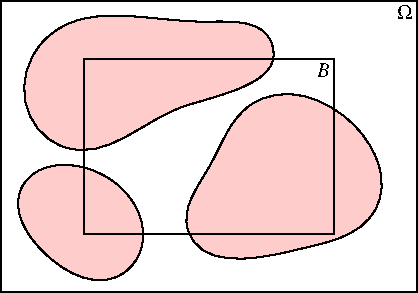
\includegraphics{images/algebra-1}
\end{center}
\caption{Ereignisalgebra mit ausgezeichneten Ereignis $B$\label{bedingt1}}
\end{figure}
\begin{figure}
\begin{center}
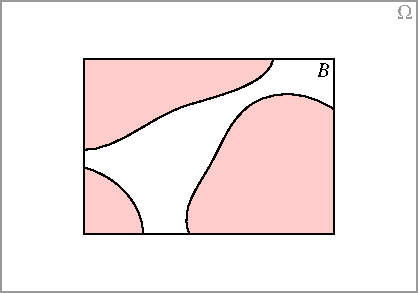
\includegraphics{images/algebra-2}
\end{center}
\caption{Ereignisalgebra wie in Abbildung \ref{bedingt1} eingeschr"ankt auf das Ereignis $B$\label{bedingt2}}
\end{figure}
In der Praxis fragt man oft nach der Verkettung von Umst"anden: hat ein
Patient bessere Heilungschancen wenn er dieses neue Medikament nimmt?
Man k"onnte das auch so formulieren: ist das Ereignis
``Patient wird gesund, unter der Voraussetzung, dass er das Medikament nimmt''
wahrscheinlicher als das Ereignis ``Patient wird gesund''? Wir m"ussen
also aus der Ereignis\-algebra der Patienten eine neue bilden, die nur
aus den Patienten besteht, welche das Medikament genommen haben.

Wenn $(\Omega, {\cal A})$ eine Ereignisalgebra ist, und 
$B\in{\cal A}$ ein Ereignis (Abbildung~\ref{bedingt1}),
dann kann man eine neue Ereignisalgebra
$(\Omega_{|B}, {\cal A}_{|B})$ wie folgt bilden (Abbildung~\ref{bedingt2}).
Die Menge der Elementarereignisse ist
\[
\Omega_{|B}=B
\]
und die Menge der Ereignisse
\[
{\cal A}_{|B}=\{A\cap B\;|\; A\in{\cal A}\}.
\]
Es w"are noch nachzupr"ufen, dass diese Menge alle Axiome einer
Ereignisalgebra erf"ullt sind\footnote{Da diese technischen Feinheiten 
f"ur die Zwecke dieses Skripts von untergeordneter Bedeutung sind, verzichten
wir auf die explizite Verifikation.}.
Diese Konstruktion macht $B$ zum sicheren Ereignis, d.~h.~in der ``Welt''
$(\Omega_{|B},{\cal A}_{|B})$ trifft $B$ immer ein (Abbildung~\ref{bedingt2}).
In $(\Omega_{|B},{\cal A}_{|B})$ muss man also davon ausgehen, dass $B$
bereits eingetroffen ist.
Man liest $\Omega_{|B}$ auch als ``$\Omega$ bedingt $B$''.

Wenn nun auf $(\Omega, {\cal A})$ eine Wahrscheinlichkeitsfunktion $P$
gegeben ist, kann man auch $P_{|B}$ bilden, indem man setzt
\begin{equation*}
P_{|B}(A)=\frac{P(A\cap B)}{P(B)},
\end{equation*}
der Nenner $P(B)$ stellt dabei sicher, dass $P_{|B}(\Omega_{|B})=P_{|B}(B)=1$.

\begin{definition}
\label{def-bedingte-wahrscheinlichkeit}
Die bedingte Wahrscheinlichkeit eines Ereignisses $A$ unter der Bedingung
$B$ ist
\[
P(A|B)=\frac{P(A\cap B)}{P(B)}.
\]
Man liest dies auch als ``Wahrscheinlichkeit von $A$ bedingt $B$''.
\end{definition}

Auch hier w"are nachzupr"ufen, dass die Rechenregeln f"ur eine
Wahrscheinlichkeitsfunktion erf"ullt sind.
Um also die Wahrscheinlichkeit in dieser Welt zu berechnen,
in der $B$ bereits eingetroffen ist, 
muss man $P(A\cap B)$ berechnen k"onnen.
Dies sollte Motivation genug sein, Rechenregeln f"ur
$P(A\cap B)$ aufzustellen, die uns bisher fehlen.

\subsection{Wahrscheinlichkeit von \texorpdfstring{$A\cap B$}{A geschnitten B}}
\begin{figure}
\begin{center}
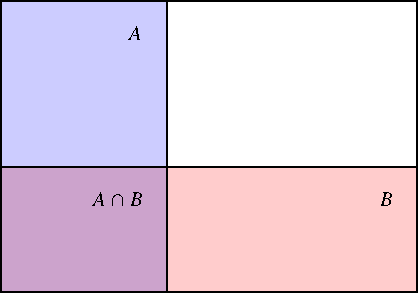
\includegraphics{images/abhaengigkeit-1}
\end{center}
\caption{Unabh"angige Ereignisse.
Die Ereignisse sind so dargestellt,
dass ihre Wahrscheinlichkeit proportional zur Fl"ache ist.
$P(A)$ und $P(B)$
entsprechen dem Teilverh"altnis, in dem $A$ bzw.~$B$ die Seite des grossen
Rechtecks teilen.
$P(A\cap B)=P(A)\cdot P(B)$\label{unabhaengig}}
\end{figure}
\begin{figure}
\begin{center}
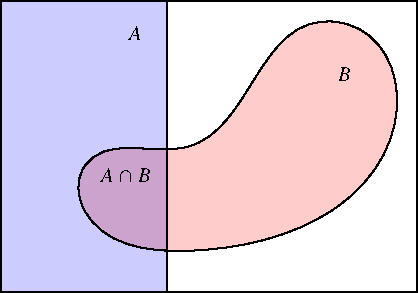
\includegraphics{images/abhaengigkeit-2}
\end{center}
\caption{Abh"angige Ereignisse.
$P(A\cap B)$ ist offensichtlich viel kleiner
als $P(A)\cdot P(B)$.
$A$ wird unwahrscheinlicher, wenn bereits $B$ eingetreten
ist.
\label{abhaengig}}
\end{figure}
Der Grund daf"ur, dass es keine einfache Rechenregel f"ur die Berechnung von 
$P(A\cap B)$ aus $P(A)$ und $P(B)$ gibt, wird mit der
Visualisierung der Ereignisse im in einem Venn-Diagramm sofort klar.
Die Elementarereignisse seien so angeordnet, dass $A$ das durch eine
vertikale Strecke abgetrennte, linke Teilrechteck von $\Omega$ ist.
Ausserdem
sollen Sie so angeordnet sein, dass die Wahrscheinlichkeit dem
Fl"acheninhalt im Diagramm entspricht.

Das Ereignis $B$ ist jetzt im Allgemeinen eine Teilmenge, die sowohl $A$ 
als auch $\bar A$ schneidet.
Die Wahrscheinlichkeit $P(A \cap B)$ entspricht
der Fl"ache der Schnittmenge im Diagramm.
Im Allgemeinen haben wir
nur aus $P(B)$ nicht gen"ugend Information um zu entscheiden, welche
``Form'' $A\cap B$ hat, wir k"onnen also nicht erwarten, dass wir $P(A\cap B)$
berechnen k"onnen.

Wenn sich $B$ ebenfalls mittels einer horizontalen Strecke als Rechteck
einzeichnen l"asst, dann ist $P(B)$ auch das Teilverh"altnis, in dem
die Strecke die vertikale Kante des Diagramms teilt.
Somit kann man $P(A\cap B)$
als Fl"acheninhalt des Schnittrechtecks berechnen: $P(A\cap B)=P(A)\cdot P(B)$.
Die Voraussetzung bedeutet, dass das Eintreffen von $B$ nicht wahrscheinlicher
oder weniger
wahrscheinlich wird, wenn $A$ eintrifft.
Das Eintreffen von $B$ h"angt also
nicht mit dem Eintreffen von $A$ zusammen.

\begin{definition}
\label{def-unabhaengige-ereignisse}
Die Ereignisse $A$ und $B$ heissen {\em unabh"angig}, wenn gilt:
\[
P(A\cap B) = P(A)\cdot P(B).
\]
\end{definition}

Beim W"urfeln sagt die Erfahrung, dass sich ein W"urfel nicht an den
letzten Wurf erinnern kann, d.~h.~der Ausgang des letzten Wurfes hat
keinen Einfluss auf den n"achsten Wurf.
Die Ereignisse ``im ersten
Wurf wird eine 5 gew"urfelt'' und ``im zweiten Wurf wird eine 6 gew"urfelt''
sind also unabh"angig.
Die Wahrscheinlichkeit, dass mit einem W"urfel
erst eine 5, dann eine 6 gew"urfelt wird, ist also
\begin{align*}
P(A\cap B)&=P(\text{``erster Wurf: 5''}\cap\text{``zweiter Wurf: 6''})\\
&=P(\text{``erster Wurf: 5''})\cdot P(\text{``zweiter Wurf: 6''})\\
&=\frac1{36}.
\end{align*}

\subsection{Bedingte Wahrscheinlichkeit}
Im vorangegangenen Abschnitt wurde bereits die bedingte Wahrscheinlichkeit
$P_{|B}(A)$ konstruiert, die wir auch
\[
P(A|B)=\frac{P(A\cap B)}{P(B)}
\]
schreiben.
Die Bedeutung des Symbols $P(A|B)$ ist die folgende.
Bei der
Bestimmung der Wahrscheinlichkeit werden nur diejenigen Experimente
ber"ucksichtigt, bei denen das Ereignis $B$ eingetreten ist.
Alle anderen Experimente interessieren nicht.

\subsubsection{Beispiel: Autounf"alle und Alkohol}
Wenn jemand sagt, 50\%
der t"odlichen Autounf"alle geschehen unter Alkoholeinfluss, dann
meint er genau genommen eigentlich folgendes.
Wir machen ein Experiment,
bei dem wir jeden Autounfall untersuchen.
Das Ereignis $T$ umfasst alle
t"odlich ausgehenden Autounf"alle, das Ereignis $A$ all jene, bei denen
Alkohol im Spiel war.
Uns interessieren jetzt nur noch die t"odlichen
Unf"alle, also die, bei denen das Ereignis $T$ eingetreten ist. 
Die anderen untersuchen wir gar nicht mehr.
Jetzt m"ochten wir die
Wahrscheinlichkeit wissen, dass Alkohol im Spiel war, aber nur noch
bei den t"odlichen Unf"allen.
Dies ist $P(A|T)$, also gilt
$P(A|T)=50\% = 0.5$.
$P(T|A)$ ist hingegen ganz etwas anderes.
Hier fragt man danach,
wie wahrscheinlich es ist, dass bei einem Autounfall unter Alkoholeinfluss
ein Toter zu beklagen ist.

\subsubsection{Beispiel: Rauchen und Lungenkrebs}
\index{Rauchen}
\index{Lungenkrebs}
In einem Zeitungsartikel gefunden: Die Wahrscheinlichkeit, dass ein Raucher
Lungenkrebs entwickelt, ist 15\%, bei einem Nichtraucher ist sie nur 1\%.
Das Experiment besteht darin, einen Menschen zu beobachten.
Einige
davon sind Raucher (Ereignis $R$), einige entwickeln Lungenkrebs (Ereignis $L$).
Betrachtet man nur die Raucher, so ist die Wahrscheinlichkeit f"ur
Lungenkrebs 15\%, also
\[
P(L|R)=0.15
\]
Betrachtet man nur die Nichtraucher, also das Ereignis $\bar R$, findet
man 
\[
P(L|\bar R)=0.01.
\]
Der Artikel liefert aber keine Auskunft dar"uber, wie viele der
Lungenkrebskranken auch Raucher sind, denn das w"are die Wahrscheinlichkeit
$P(R|L)$.

\subsubsection{Zusammenhang zwischen \texorpdfstring{$P(A\cap B)$}{P(A geschnitten B)}, \texorpdfstring{$P(A|B)$}{P(A bedingt B)} und \texorpdfstring{$P(B|A)$}{P(B bedingt A)}}
In allen drei F"allen geht es um die Wahrscheinlichkeit des Eintretens
von $A$ und von $B$, allerdings jeweils in verschiedenem
Zusammenhang.
\begin{center}
\begin{tabular}{|c|l|c|}
\hline
Wahrscheinlichkeit&"Ubersetzung&Scope\\
\hline
$P(A\cap B)$&\strut Wahrscheinlichkeit, dass $A$ und $B$ eintreten\strut &$\Omega$\\
%\hline
$P(A|B)$&\begin{minipage}[t]{3.0in}\strut Wahrscheinlichkeit, dass $A$ eintritt, wenn $B$ schon eingetreten ist\strut \end{minipage}&$B$\\
%\hline
$P(B|A)$&\begin{minipage}[t]{3.0in}\strut Wahrscheinlichkeit, dass $B$ eintritt, wenn $A$ schon eingetreten ist\strut \end{minipage}&$A$\\
\hline
\end{tabular}
\end{center}
(Vergleiche auch Abbildung~\ref{condprob}.)
\begin{figure}
\begin{center}
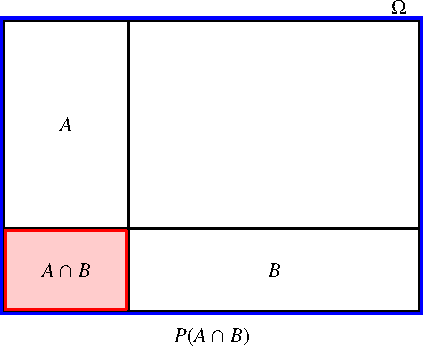
\includegraphics[width=0.3\hsize]{images/abhaengigkeit-3}\quad
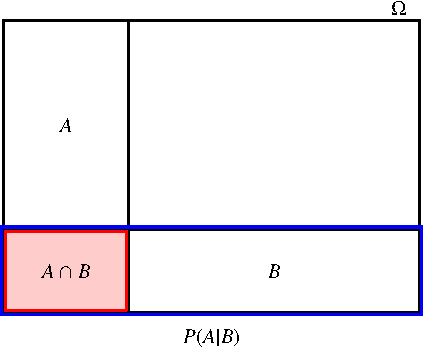
\includegraphics[width=0.3\hsize]{images/abhaengigkeit-5}\quad
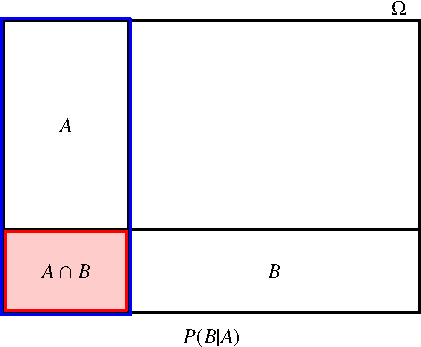
\includegraphics[width=0.3\hsize]{images/abhaengigkeit-4}
\end{center}
\caption{Wahrscheinlichkeit von $A\cap B$ in jeweils anderer Umgebung
\label{condprob}}
\end{figure}

\subsection{Zerlegung eines Wahrscheinlichkeitsraumes}
Der
Begriff der bedingten Wahrscheinlichkeit erm"oglicht,
ein Wahrscheinlichkeitsproblem in m"oglicherweise einfachere, jedenfalls
kleinere Probleme zu zerlegen.
Wenn bei einem Experiment zwei Zust"ande
eintreten, die sich gegenseitig ausschliessen, k"onnen wir die 
Wahrscheinlichkeit bestimmen, unter denen die weiteren Resultate
des Experiments eintreten, jedoch unter der Vorbedingung, dass einer
der benannten Zust"ande bereits eingetreten ist.
Wenn wir nun auch
noch die Wahrscheinlichkeit jedes Zustandes kennen, m"usste es doch
m"oglich sein, auch die Wahrscheinlichkeit der weiteren Resultate zu
ermitteln.
% TODO Missing Example
Im obigen Beispiel der Meinungsumfrage ist anschaulich klar, dass man die
Wahrscheinlichkeit f"ur ``Ja'' berechnen kann, wenn man einerseits die
Wahrscheinlichkeit f"ur ``Ja'' in  jeder Altersklasse kennt, und andererseits
weiss, wie die Altersklassen in der Bev"olkerung verteilt sind.

\begin{figure}
\begin{center}
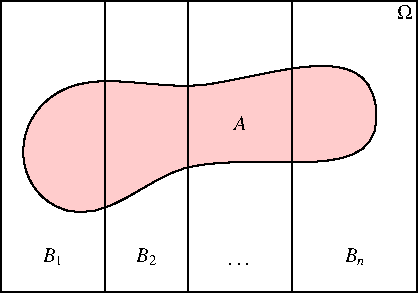
\includegraphics{images/total-1.pdf}
\end{center}
\caption{Wahrscheinlichkeitsraum $\Omega$, der sich in die in die
Ereignisse $B_1,B_2,\dots,B_n$ zerlegen l"asst.\label{zerlegung}}
\end{figure}
Wir versuchen, das etwas formaler zu schreiben
(siehe Abbildung \ref{zerlegung}):
Sind $B_i$ mit $1\le i$ paarweise
disjunkte Ereignisse
in einer Ereignisalgebra $(\Omega,{\cal A})$, f"ur welche ausserdem
gilt
\[
\bigcup_{i=0}^{n}B_i = \Omega,
\]
dann kann man die Wahrscheinlichkeit von $A$ aus den bedingten
Wahrscheinlichkeiten der Teile $A\cap B_i$ und $B_i$ wieder zusammensetzen.
Bekannt sind die Wahrscheinlichkeiten
$P(B_i)$, die Wahrscheinlichkeit der Zust"ande, und
$P(A|B_i)$, die Wahrscheinlichkeit, dass $A$ eintritt, unter der Bedingung
das $B_i$ bereits eingetreten ist.
Nach Definition ist $P(A|B_i)=P(A\cap B_i)/P(B_i)$, also
$P(A|B_i)\cdot P(B_i) = P(A\cap B_i)$.
Die Vereinigung der Ereignisse $A\cap B_i$ ist
\[
\bigcup_{i=0}^{n} A\cap B_i=A\cap\bigcup_{i=0}^{n}B_i=A,
\]
und die Mengen $A\cap B_i$ sind disjunkt.
Also kann man die Summe ihrer
Wahrscheinlichkeiten mit der Additionsformel ausrechnen:
\[
\sum_{i=0}^{n}P(A\cap B_i)=P\biggl(\bigcup_{i=0}^{n}A\cap B_i\biggr)=P(A).
\]
Andererseits
haben wir oben bereits $P(A\cap B_i)$ bestimmt, wir k"onnen
also einsetzen und erhalten:
\[
P(A)=\sum_{i=0}^{n}P(A|B_i)\cdot P(B_i).
\]
Somit l"asst sich tats"achlich die Wahrscheinlichkeit eines Ereignisses
aus den bedingten Wahrscheinlichkeiten und den Wahrscheinlichkeiten
der Bedingungen errechnen.
Wir fassen diese Erkenntnis in folgendem Satz zusammen.
\index{Wahrscheinlichkeit!totale}
\begin{satz}
Ist $B_i$ eine Folge paarweise disjunkter Mengen mit $\bigcup_{i=0}^{n}B_i=\Omega$, dann gilt f"ur jedes Ereignis $A$
\[
P(A)=\sum_{i=0}^{n}P(A|B_i)\cdot P(B_i).
\]
\end{satz}
Dieser Satz heisst auch der {\em Satz von der totalen Wahrscheinlichkeit},
da er die Wahrscheinlichkeit eines Ereignisses aus den bedingten
Wahrscheinlichkeiten unter verschiedenen Voraussetzungen und der
Wahrscheinlichkeit des Eintretens dieser Voraussetzungen rekonstruiert.
Dieser Satz ist die ``wahrscheinlichkeitstheoretisch Form einer
Fallunterscheidung'': man kennt die F"alle $B_i$, und deren Wahrscheinlichkeit
$P(B_i)$, sowie die Wahrscheinlichkeit $P(A|B_i)$, dass $A$ im Falle 
$B_i$ eintritt.
Die Formel "uber die totale Wahrscheinlichkeit
liefert daraus wieder $P(A)$.

Wir bemerken noch, dass es gar nicht unbedingt n"otig ist, dass die Mengen
$B_i$ ganz $\Omega$ aussch"opfen, es w"urde auch
gen"ugen, wenn die Wahrscheinlichkeit $0$ ist, dass $A$ eintritt
unter der Bedingung,
dass bereits $\bigcup_{i=0}^{n}B_i$ eingetreten ist.
F"ur den
Experimentator bedeutet das, dass er nur jene Vorbedingungen $B_i$
ber"ucksichtigen muss, unter denen sein Experiment ``funktioniert'',
alle anderen m"oglichen Zust"ande haben keinen Einfluss auf
die Wahrscheinlichkeit seiner Resultate.
Man darf beim Experimentieren also durchaus einzelne Resultate
verwerfen, wenn man weiss, was man tut!

\subsubsection{Studienerfolg}
Die folgenden Zahlen sind erfunden, und dienen nur der Illustration
des Prinzips.
Eine Statistik hat die Wahrscheinlichkeit f"ur den
Studienerfolg untersucht, und folgende Resultate erhalten.
Die Studierenden setzen sich zusammen aus 60\% BMS, 30\% Kantonssch"uler
und "Ubertritte von anderen Hochschulen.
Die Wahrscheinlichkeit
das Studium erfolgreich abzuschliessen, ist f"ur BMS 80\%,
f"ur Kantonssch"uler 90\%, 85\% f"ur die "Ubertreter von anderen
Hochschule.
Wie gross ist die Wahrscheinlichkeit f"ur den Studienerfolg?

$\Omega$ ist die Menge aller Studienversuche.
60\% davon bilden das
Ereignis $B$ bestehend aus Studienversuchen, die im Anschluss an die BMS
erfolgen.
30\% machen das Ereignis $K$ mit den Kanti-Abg"angern aus,
10\% das Ereignis $A$ mit "Ubertritten von anderen Hochschulen.
Es ist klar, dass 
\[
\Omega = B \cup K\cup A.
\]
Gefragt ist die Wahrscheinlichkeit des Ereignisses $E$, welches
die erfolgreich abgeschlossenen Studienversuche beinhaltet.
F"ur die Wahrscheinlichkeit gilt nach dem Satz "uber die totale
Wahrscheinlichkeit
\begin{align*}
P(E)&=P(E|B)P(B)+P(E|K)P(K)+P(E|A)P(A).
\\
    &= 80\%\cdot 60\%
     + 90\%\cdot 30\%
     + 85\%\cdot 10\%
\\
&=0.8\cdot 0.6 + 0.9 \cdot 0.3 + 0.85 \cdot 0.1 = 0.835
\end{align*}

\subsubsection{W"urfelspiel}
Wir betrachten nochmals das Beispiel W"urfeln mit zwei W"urfeln, wobei
bei einem Pasch im ersten Wurf noch genau einmal gew"urfelt wird.
Wir m"ochten die Wahrscheinlichkeit berechnen, dass die totale Augensumme
mindestens 10 ist.
Wir nennen dieses Ereignis $Z$.

Zun"achst kann man unterteilen f"ur den Fall, dass im ersten Wurf
ein Pasch (Ereignis $P$) geworfen wird.

Es gilt nach dem Satz "uber die totale Wahrscheinlichkeit
\[
P(Z) = P(Z|P) P(P) + P(Z|\bar P) P(\bar P).
\]
Selbstverst"andlich ist $P(\bar P)=1-P(P)$, so dass man $P(Z)$ bereits
vereinfachen kann:
\[
P(Z) = P(Z|P) P(P) + P(Z|\bar P) (1-P(P)).
\]
Man kann aber das Ereignis $P$ noch weiter unterteilen in die
Ereignisse $P_k$, mit $1\le k\le 6$, also
\begin{align*}
P(P)&=
P(P_1)+
P(P_2)+
P(P_3)+
P(P_4)+
P(P_5)+
P(P_6)
\\
P(Z|P)
&=
P(Z|P_1)P(P_1|P)+
P(Z|P_2)P(P_2|P)+
P(Z|P_3)P(P_3|P)
\\
&\qquad +
P(Z|P_4)P(P_4|P)+
P(Z|P_5)P(P_5|P)+
P(Z|P_6)P(P_6|P)
\end{align*}
Die Ereignisse haben wir auch fr"uher schon untersucht, daraus kann
man einige Wahrscheinlichkeiten bereits ablesen:
\begin{align*}
P(Z|P_6)&=1\\
P(Z|P_5)&=1\\
P(Z|P_4)&=1
\end{align*}
denn in allen diesen F"allen erreicht man mit dem zweiten Wurf mit
Sicherheit zehn oder mehr.

\subsection{Ziegen und Autos} \label{ziegen:autos}
Marylin vos Savant hat in einer Kolumne ein Gedankenexperiment vorgestellt.
In einer Quiz-Show muss der Kandidat eine von drei T"uren w"ahlen, wobei
sich hinter einer der T"uren ein Auto versteckt, hinter den anderen Zweien
ein Ziege.
Das Ziel des Spiels ist, das Auto zu gewinnen.
Nach der Wahl
durch den Kandidaten "offnet der Quizmaster eine der T"uren, hinter der sich
eine Ziege befindet, nicht aber die T"ur, die der Kandidat gew"ahlt hat.
Der Kandidat hat jetzt nochmals die M"oglichkeit, die T"ur zu wechseln.
Welche Strategie soll er w"ahlen.
Bei der ersten Auswahl bleiben, oder
wechseln?

Um die Frage zu beantworten berechnen wir die Gewinnwahrscheinlichkeit
f"ur jede der Strategien.
Zun"achst die ``Bleibe''-Strategie.
Es ist die
Wahrscheinlichkeit f"ur einen Gewinn $P(G)$ auszurechnen.
Hinter der zun"achst
gew"ahlten T"ur kann sich ein Auto (Ereignis $A$) befinden, oder eine Ziege
(Ereignis $Z$).
Es ist nat"urlich $A\cap Z=\emptyset$ und $A\cup Z=\Omega$.
Also gilt
\begin{equation}
P(G)=P(G|A) P(A) + P(G|Z)P(Z).
\label{ziegenformel}
\end{equation}
Nat"urlich ist $P(A)=\frac13$ und $P(Z)=\frac23$.
$P(G|A)$ ist die Wahrscheinlichkeit mit der ``Bleibe''-Strategie zu
gewinnen, wenn hinter der zun"achst gew"ahlten T"ur ein Auto war: diese
ist nat"urlich $1$.
Ebenso verliert man mit Sicherheit, wenn hinter der
T"ur eine Ziege war: $P(G|Z)=0$, also
\[
P(G)=P(G|A)P(A)+P(G|Z)P(Z)=1\cdot \frac13 + 0\cdot\frac 23=\frac13.
\]

F"ur die ``Wechsel''-Strategie gilt nat"urlich auch die Formel
\ref{ziegenformel}, aber die bedingten Wahrscheinlichkeiten sind verschieden.
Wenn man ein Auto gew"ahlt hatte, und wechselt, verliert man, also $P(G|A)=0$.
Hat man ein Ziege erwischt, und wechselt, bekommt man das Auto, denn die
zweite Ziege kann man ja nicht erwischen, deren T"ur hat der Quiz-Master
ge"offnet.
Also ist $P(G|Z)=1$.
Somit folgt jetzt
\[
P(G)=P(G|A)P(A)+P(G|Z)P(Z)=0\cdot\frac13+1\cdot\frac23=\frac23.
\]
Mit der Wechselstrategie ist also die Wahrscheinlichkeit, zu gewinnen,
doppelt so gross, wechseln lohnt sich also auf jeden Fall.


\subsection{Wahrscheinlichkeitsvektoren und -matrizen}
Der Satz von der totalen Wahrscheinlichkeit kann auch in Matrixform
geschrieben werden:
\begin{align*}
P(A)&=P(A|B_1)P(B_1)+\dots+P(A|B_n)P(B_n)
=
\begin{pmatrix}
P(A|B_1)&\dots&P(A|B_2)
\end{pmatrix}
\begin{pmatrix}
P(B_1)\\\vdots\\P(B_n)
\end{pmatrix}
\end{align*}
Der Spaltenvektor
\[
\begin{pmatrix}
P(B_1)\\\vdots\\P(B_n)
\end{pmatrix}
\]
hat die Eigenschaften, dass alle seine Eintr"age zwischen $0$ und $1$
liegen, und ihre Summe $1$ gibt.
\index{Wahrscheinlichkeitsvektor}
Ein solcher Vektor heisst {\it Wahrscheinlichkeitsvektor}.

Die Matrizenschreibweise erlaubt, auch die totalen Wahrscheinlichkeiten
f"ur mehrere Ereignisse $A_1,\dots,A_m$ gleichzeitig zu berechnen:
\[
\begin{pmatrix}
P(A_1)\\
P(A_2)\\
\vdots\\
P(A_m)
\end{pmatrix}
=
\begin{pmatrix}
P(A_1|B_1) & P(A_1|B_2) & \dots &P(A_1|B_n)\\
P(A_2|B_1) & P(A_2|B_2) & \dots &P(A_2|B_n)\\
\vdots     & \vdots     & \ddots&\vdots\\
P(A_m|B_1) & P(A_m|B_2) & \dots &P(A_m|B_n)\\
\end{pmatrix}
\begin{pmatrix}
P(B_1)\\
P(B_2)\\
\vdots\\
P(B_n)
\end{pmatrix}
\]
Sind die Ereignisse $A_i$ ebenfalls paarweise disjunkt und decken ganz
$\Omega$ ab, dann sind auch die Spalten von der Matrix $(P(A_i|B_j))$
jeweils Wahrscheinlichkeitsvektoren.
\index{Wahrscheinlichkeitsmatrix}
Eine solche Matrix heisst {\it Wahrscheinlichkeitsmatrix}.

\subsection{Satz von Bayes} \label{satz-von-bayes}
\index{Bayes, Satz von}
F"ur zwei beliebige Ereignisse mit $A$ und $B$ mit nicht verschwindender
Wahrscheinlichkeit gilt
\[
P(A|B)\cdot P(B)= P(A\cap B)=P(B|A)\cdot P(A),
\]
und es folgt
\[
P(A|B)=\frac{P(B|A)\cdot P(A)}{P(B)}.
\]
Dieser Zusammenhang ist bekannt als der Satz von Bayes:
\begin{satz}[Satz von Bayes]
F"ur zwei Ereignisse $A$ und $B$ mit $P(B)\ne0$ gilt
\[
P(A|B)=\frac{P(B|A)\cdot P(A)}{P(B)}.
\]
\end{satz}
Die Bedeutung dieses Satzes besteht darin, dass er die Schlussrichtung
umzukehren erlaubt.
Die bedingte Wahrscheinlichkeit $P(A|B)$ ist ja die
Wahrscheinlichkeit, dass ein das Ereignis $A$ eintritt, wenn $B$ bereits
eingetreten ist.
Sie erlaubt, eine Wette einzugehen, dass $A$ eintreten
wird, wenn $B$ bereits eingetreten ist.
Der Satz von Bayes erm"oglicht
also, auch eine Wette f"ur $B$ einzugehen, wenn $A$ bereits eingetreten
ist.
Im Gegensatz zur Schlussweise in der Logik, die niemals umkehrbar ist,
kann man auf Wahrscheinlichkeiten basierende Schl"usse umkehren.

\subsubsection{Was bedeutet ein positiver HIV-Test?}
\begin{figure}
\begin{center}

\includegraphics[width=\hsize]{graphics/aids-300}
\end{center}
\caption{``Blick am Abend'' vom 12.~August 2008\label{aids}}
\end{figure}
Im ``Blick am Abend'' vom 12.~August 2008 erschien der Artikel in Abbildung 
\ref{aids} mit dem Titel ``Warum uns Wahrscheinlichkeiten verwirren''.
Darin ist von folgenden Ereignissen die Rede, die sich auf sich nicht riskant
verhaltende M"anner ($=\Omega$) beziehen.
\index{HIV-Test}
\begin{enumerate}
\item Ereignis $H$: Ein Mann ist HIV-infiziert.
\item Ereignis $T$: ein HIV-Test ergibt ein positives Resultat.
\end{enumerate}
Der Artikel teilt uns zudem ein paar Wahrscheinlichkeiten mit:
\begin{itemize}
\item HIV-Rate bei M"annern, die sich nicht riskant verhalten:
$P(H)=0.0001$.
\item Wahrscheinlichkeit, dass bei einer infizierten Person der Test
ein positives Resultat ergibt: $P(T|H)=0.999$.
\item Wahrscheinlichkeit, dass bei einer gesunden Person der Test negativ
ist: $P(\bar T|\bar H)=0.9999$.
\end{itemize}
Wie gross ist die Wahrscheinlichkeit, dass ein sich nicht riskant verhaltender
Mann tats"achlich HIV hat, wenn er einen positiven HIV-Test hat? Wie
gross ist $P(H|T)$?

Der Satz von Bayes liefert die Antwort:
\begin{equation}
P(H|T)=\frac{P(T|H)\cdot P(H)}{P(T)}
\label{aidsprobability}
\end{equation}
Darin sind fast alle Gr"ossen direkt aus dem Artikel ablesbar, nur $P(T)$ muss
noch bestimmt werden.
Dazu dient der Satz "uber die totale Wahrscheinlichkeit,
den wir auf die Tatsache anwenden, dass ein sich nicht riskant verhaltender
Mann entweder HIV hat oder nicht: $\Omega=H\cup \bar H$.
\begin{align*}
P(T)
&=P(T|H)\cdot P(H)+P(T|\bar H)\cdot P(\bar H)\\
&=P(T|H)\cdot P(H)+(1-P(\bar T|\bar H))\cdot (1 - P(H))\\
&=0.999\cdot 0.0001+(1-0.9999)\cdot(1-0.0001)\\
&=0.00019989\simeq 0.0002
\end{align*}
Eingesetzt in (\ref{aidsprobability}) ergibt sich jetzt das Resultat
\[
P(H|T)=\frac{0.999\cdot 0.0001}{0.0002}=.4995\simeq 0.5
\]
oder mit anderen Worten, auch wenn der HIV-Test positiv ist, ist
die Wahrscheinlichkeit f"ur einen sich nicht riskant verhaltenden Mann,
tats"achlich HIV-infiziert zu sein, nur $50\%$.


\input spamfilter.tex
\input google.tex
%SourceDoc ws-skript.tex
%
% c03-erwartung.tex
%
% (c) 2006 Prof. Dr. Andreas Mueller
% $Id: c03-erwartung.tex,v 1.18 2008/11/02 00:12:44 afm Exp $
%
\rhead{Erwartung und Varianz}
\chapter{Erwartungswert und
Varianz\label{chapter-erwartungswert-und-varianz}} F"ur den
\marginpar{\tiny\raggedright Erwarteter Gewinn im Casino}
\index{Casino}
Casinobetreiber ist die genaue Wahrscheinlichkeit eines Ereignisses
nur von sekund"arem Interesse. Sein Betrieb ist genau dann rentabel,
wenn im Mittel, "uber viele Spiele, die Spieler mehr Geld in seinem
Etablissement liegen lassen als er an Gewinnen auszahlen muss.
Zun"achst wird er sich dazu Gedanken machen, welchen Gewinn jede
einzelne Spielsituation f"ur ihn ergibt. Zusammen mit der
Wahrscheinlichkeit des Eintretens dieser Situation wird er abzusch"atzen
versuchen, wie gross sein Gewinn im Mittel sein wird.

Ganz "ahnlich geht es dem Experimentator, der eine Messung mehrmals
durch\-f"uhrt.  Er kann nicht davon ausgehen, dass jede Messung das
gleiche Resultat liefert.  Jede einzelne Messung ist
ein Wahrscheinlichkeitsexperiment mit einer sehr
grossen Zahl von Einfl"ussen, die alle nicht bekannt sind. Der
Experimentator wird versuchen, aus einer grossen Zahl von Messresultaten
einen besonders wahrscheinlichen f"ur die gemessene Gr"osse zu
ermitteln. Trotzdem wird die Genauigkeit des so ermittelten Wertes
\marginpar{\tiny\raggedright Erwartungswert und Streuung bei Messwerten}
unbekannt sein. Es sollte aber mindestens m"oglich sein, aus der
``Streuung'' der Messwerte eine Gr"osse abzuleiten, die ein Aussage
"uber die Genauigkeit des gefundenen Wertes macht.

Ein
\marginpar{\tiny\raggedright Motivationsbeispiel: Durschnittsnoten}
\index{Durchschnitt}
Sch"uler hat f"unf Pr"ufungen geschrieben, und dabei die Noten
3, 3, 5, 3, 6 erhalten. Die Gesamtnote sollte die Semesterleistung
wiedergeben. Sie soll das repr"asentieren, was man bei einer
erneuten Durchf"uhren einer Pr"ufung erwarten w"urde. Nat"urlich
ist dies kein mathematisch klar gefasster Begriff: man k"onnte auf
verschiedene zweckm"assige Resultate kommen:
\begin{enumerate}
\item Im Durchschnitt hat der Sch"uler die Note 4 erreicht, diesen Wert
betrachtet man als repr"asentativ f"ur das Semester.
\item Offensichtlich hat sich der Sch"uler gegen Ende des Semsters
gesteigert, wie man das berechnen will ist zwar noch nicht klar,
aber eine 5 w"are wohl etwa angemessen.
\item 3 ist die h"aufigste Note, also wird er wohl auch das n"achste
mal wieder eine 3 schreiben.
\item Eine 6 und eine 3 betrachten wir als Ausreisser, dann ist die
Durchschnittsnote 3.7.
\end{enumerate}
Keines dieser Argumente ist wirklich falsch, trotzdem verwendet man
in der Praxis eigentlich nur die erste L"osung. Warum?

\section{Zufallsvariable}
\index{Zufallsvariable}
Wenn wir von ``im Mittel zu erwartendem Ausgang'' sprechen wollen, brauchen
wir Versuchsresultate, die sich auch tats"achlich ``mitteln'' lassen.
Elementarereignisse sind Realisierungen eines Versuchs und somit der
rechnerischen Verkn"upfung nicht zug"anglich.
Somit muss den Elementarereignissen
ein Wert in einem Wertebereich zugeordnet werden, in dem
Berechnungen m"oglich sind.

\subsection{Wurf eines W"urfels}
Wirft man einen W"urfel, zeigt dieser ein Bild mit einem oder mehreren Punkten, 
dies sind die Elementarereignisse:
\[
\Omega = \{
\epsdice{1},
\epsdice{2},
\epsdice{3},
\epsdice{4},
\epsdice{5},
\epsdice{6}
\}.
\]
Leute, die Zahlen kennen, k"onnen diese Bilder auch als Zahlen interpretieren.
Sie verwenden die Abbildung
\[
X\colon \Omega \to \{1,2,3,4,5,6\}
\]
mit den Werten
\begin{align*}
\epsdice{1}&\mapsto 1,\\
\epsdice{2}&\mapsto 2,\\
\epsdice{3}&\mapsto 3,\\
\epsdice{4}&\mapsto 4,\\
\epsdice{5}&\mapsto 5,\\
\epsdice{6}&\mapsto 6.
\end{align*}
Dass diese Zuordnung von Elementarereignissen zu Zahlenwerten tats"achlich
ein zus"atzlicher Schritt ist, sieht man zum Beispiel auch daran, dass
in Spielen f"ur Kinder, die die Zahlen noch nicht kennen, Farbw"urfel
verwendet werden, und keine Zuordnung von Zahlenwerten vorgenommen wird.

Die Menge $\Omega$ der Elementarereignisse beschreibt alle m"oglichen W"urfe
des W"urfels. Wenn wir uns nur f"ur die gezeigte Augenzahl interessieren,
brauchen wir eine Funktion, welche jedem Elementarereignis diesen speziellen
Ausgang zuordnet:
\[
X: \Omega\to{\mathbb Z}: \omega\mapsto X(\omega)
\]
Eine solche Abbildung heisst eine Zufallsvariable.
Mit Hilfe der Zufallsvariable kann man jetzt das Ereignis, dass eine Sechs
gew"urfelt wurde, auch so formulieren:
\[
A_6=\{\omega\in\Omega\;|\;X(\omega) = 6\}.
\]
In $\mathbb{Z}\subset\mathbb{R}$ kann nat"urlich gerechnet werden, und
auch eine intuitive Vorstellung davon, was ``im Mittel'' etwa heissen
k"onnte, ist bereits vorhanden.

\subsection{Definition}
Zufallsvariable sind als Funktionen, die Elementarereignissen Werte zuordnen.
Daher k"onnten wir als Definition verwenden
\begin{definition}
Eine Zufallsvariable $X$ ist eine Funktion $X\colon \Omega\to\mathbb R$.
\end{definition}

Wir erarten nat"urlich, dass die Mengen
\begin{align*}
A&=\{\omega\in\Omega\,|\,X(\omega)=a\}\\
B&=\{\omega\in\Omega\,|\,b\le X(\omega)\le c\}
\end{align*}
Ereignisse sind.
Da wir uns "uber die mengentheoretischen Vorasussetzugen an Ereignisse
kaum Gedanken gemacht haben, ist dies f"ur uns keine Einschr"ankung,
aber die technisch korrekte Definition w"are:

\begin{definition}
Eine Zufallsvariable $X$ ist eine Funktion $X\colon \Omega\to \mathbb R$,
die zus"atzlich die Eigenschaft hat, dass die Mengen 
$\{\omega | X(\omega) < x\}$ Ereignisse sind.
\end{definition}

Im Einf"uhrungsbeispiel ist $\Omega$ die Menge aller m"oglichen
Pr"ufungen, $\omega\in\Omega$ ist eine einzelne Pr"ufung, und $X(\omega)$
ist die Note, die diese Pr"ufung erzielt hat.

Selbstverst"andlich k"onnen Zufallsvariable auch andere Wertebereiche haben.
Eine Abbildung $X:\Omega\to W$ ist eine $W$-wertige Zufallsvariable.
Alle Operationen im Wertebereich sind auch f"ur Zufallsvariable m"oglich.
Kann man im Wertebereich $W$ addieren, dann ist auch die Summe zweier
Zufallsvariable $X_1$ und $X_2$ definiert durch
\[
X_1+X_2:\Omega\to W:\omega\mapsto(X_1+X_2)(\omega) := X_1(\omega) + X_2(\omega),
\]
und entsprechend f"ur alle anderen Operationen in $W$.

Bei einer analogen Messung ist zum Beispiel jeder beliebige reelle
Wert m"oglich, eine reelle Zufallsvariable w"are demnach eine Abbildung
\[
X:\Omega\to\mathbb R:\omega\mapsto X(\omega)\in\mathbb R.
\]
Die Messung von Strom und Spannung an einem Verbraucher definiert zwei
Zufallsvariable $I:\Omega\to\mathbb R$ und $U:\Omega\to U$. Die vom Verbraucher
verbrauchte Leistung ist die Zufallsvariable
\[
U\cdot I:\Omega\to\mathbb R: \omega\mapsto (U\cdot I)(\omega) = U(\omega)I(\omega).
\]
Eine komplexe Zufallsvariable w"are die Impedanz
\index{Impedanz}
\[
Z:\Omega\to\mathbb C:\omega\mapsto Z(\omega)\in\mathbb C,
\]
Realteil $\operatorname{Re}Z$ und Imagin"arteil $\operatorname{Im}Z$
sind ebenfalls zwei Zufallsvariablen,
f"ur die $Z=\operatorname{Re}Z + i \operatorname{Im}Z$ gilt.

Da im Folgenden aber auch mit Wahrscheinlichkeiten gerechnet werden soll,
m"ussen
Zufallsvariablen zus"atzlich dazu verwendet werden k"onnen, Ereignisse zu
beschreiben.
Mann m"ochte zum Beispiel bei einer Spannungsmessung
$U\colon\Omega\to\mathbb{R}$ das Ereignis
$A=\{\omega\in\Omega\;|\;210\le U(\omega)\le 250\}$
verwenden, und seine Wahrscheinlichkeit berechnen k"onnen. Dazu ist es
notwendig, dass $A\in{\cal A}$ ein Ereignis ist. Meist werden uns interessierende
Zufallsvariable Werte in $\mathbb{R}$ haben, und Ereignisse von der
Form $\{\omega\;|\;X(\omega)\in I\subset\mathbb{R}\}$ sein.
Aus den Intervallen $I\subset\mathbb{R}$ wird aber, wie wir bereits wissen, eine
zweckm"assige Ereignisalgebra $(\mathbb{R},{\cal R})$ erzeugt. Somit ist
die Forderung, dass $\{\omega\;|\;X(\omega)\in I\}=X^{-1}(I)$ ein Ereignis sein
soll, nur ein Spezialfall der Forderung, dass $X^{-1}(B)\in{\cal A}$ sein
soll f"ur jedes interessante Ereignis $B$ im Wertebereich. Es w"are also gut,
wenn Zufallsvariable grunds"atzlich immer als Wertebereich eine Ereignisalgebra
haben, nicht nur eine Menge. Daraus ergibt sich die allgemeine Definition
der Zufallsvariable.

\begin{definition}\marginpar{\tiny\raggedright Definition Zufallsvariable}Sind $(\Omega,{\cal A})$ und $(\Upsilon,{\cal B})$
Ereignisalgebren, dann heisst eine Abbildung $X\colon\Omega\to\Upsilon$
eine {\bf Zufallsvariable}, wenn $X^{-1}(B)\in{\cal A}$ f"ur alle $B\in{\cal B}$.
\end{definition}

"Ublicherweise sind die Ereignisalgebren so gew"ahlt, dass diese Bedingung
mehr oder weniger automatisch erf"ullt ist.

\section{Erwartungswert\label{section-erwartungswert}}
\index{Erwartungswert}
\subsection{Motivation}
\subsubsection{Gewinn beim M"unzwurf}
Wir spielen das folgende einfache Wahrscheinlichkeitsexperiment.
\marginpar{\tiny\raggedright ``Kopf oder Zahl''-Spiel}
In jeder Runde setzen wir einen Einsatz von einem Franken auf den
Ausgang ``Kopf'' oder ``Zahl'' des Wurfes mit einer fairen M"unze.
Setzen wir richtig, erhalten wir den Einsatz zur"uck, zeigt die
M"unze das andere Resultat, verlieren wir den Einsatz. Die Zufallsvariable
$X(\omega)$ soll den Gewinn beim Eintreffen des Ereignisses $\omega$
angeben.

Im
\marginpar{\tiny\raggedright erwarteter Gewinn}
langfristigen Mittel erwarten wir, dass wir in etwa der H"alfte
der F"alle gewinnnen, in der anderen H"alfte verlieren. Im Mittel
m"ussen wir daher davon ausgehen, dass wir pro M"unzwurf einen
halben Franken gewinnen. Der erwartete Gewinn einem einzelnen
Wurf w"are also $E(X)=0.5$.

Wir versuchen dieses Experiment zu formalisieren. Die zugeh"orige
Wahrscheinlichkeitsalgebra kennt nur zwei interessante Ereignisse,
$\{\text{``Kopf''}\}$ oder $\{\text{``Zahl''}\}$.
Die Ereignisse, ihre Wahrscheinlichkeiten und wo sinnnvoll
die zu erwartenden Gewinne sind
in der Tabelle \ref{kopfzahlwahrscheinlichkeit} dargestellt.
\begin{table}
\begin{center}
\begin{tabular}{|c|c|c|}
\hline
Ereignis&Wahrscheinlichkeit&Gewinn\\
\hline
$\{\text{``Kopf''}\}$&0.5&0\\
$\{\text{``Zahl''}\}$&0.5&1\\
$\emptyset$&0&\\
$\Omega$&1&\\
\hline
\end{tabular}
\end{center}
\caption{Wahrscheinlichkeit und Gewinn bei ``Kopf oder Zahl''
\label{kopfzahlwahrscheinlichkeit}}
\end{table}
Die beiden Ereignisse $\{\text{``Kopf''}\}$ und $\{\text{``Zahl''}\}$
decken offenbar alle M"oglichkeiten ab, und innerhalb des Ereignisses
ist der Gewinn einheitlich. Der erwartete Gewinn ist also:
\[
E(\text{``Gewinn''})=\text{``Gewinn bei Kopf''}\cdot P(\text{``Kopf''})
+\text{``Gewinn bei Zahl''}\cdot P(\text{``Zahl''})
\]
Wenn etwas allgemeiner ein Spiel in $n$ verschiedene m"ogliche
Ausg"ange (Ereignisse) $A_i$ unterteilt werden kann, die je den
Gewinn $g_i$ liefern, dann ist der erwartete Gewinn
\[
E=\sum_{i=1}^{n}g_iP(A_i).
\]

\subsubsection{Notenschnitt}
Im Beispiel des Sch"ulers m"ussten wir also zun"achst Ereignisse
identifizieren, und den Gewinn bestimmen, den der Sch"uler hat, wenn
dieses Ereignis eintritt. Das Ereignis $A_n=\{\text{``Note $n$''}\}$
beschreibt den Fall, dass der Sch"uler die Note $n$ erreicht hat.
Aus den experimentellen Daten leiten wir ab, dass die Wahrscheinlichkeiten
f"ur die einzelnen Ereignisse die folgenden sind:
\begin{eqnarray*}
P(A_1)&=&0\\
P(A_2)&=&0\\
P(A_3)&=&\frac35\\
P(A_4)&=&0\\
P(A_5)&=&\frac15\\
P(A_6)&=&\frac15\\
\end{eqnarray*}
Als
\marginpar{\tiny\raggedright Durchschnittsnote als Erwartungswert der Note}
``Gewinn'' beim Eintreten des Ereignisses k"onnen wir die Note
ansehen, d.h. der Erwartungswert ist 
\[
E=\frac35\cdot 3 + \frac15\cdot 5 + \frac15\cdot 6=\frac{3\cdot 3+ 1\cdot5 + 1\cdot6}{5},
\]
also genau das, was der ``Notendurchschnitt'' auch angibt.

\subsection{Erste Definition und Rechenregeln}
Diese Beispiele f"uhren uns auf folgende abstrakte Definition,
die in den folgenden Abschnitten
konkretisiert werden soll.

\begin{definition}\marginpar{\tiny\raggedright Definition Erwartungswert}
Sei $X$ eine Funktion auf $\Omega$, und lasse sich $\Omega$ in endlich
viele Ereignisse $A_i$ zerlegen, auf denen $X(\omega)$ konstant ist,
dann ist der {\bf Erwartungswert} von $X$
\[
E(X)=\sum_{i=0}^nP(A_i)\cdot X(A_i)
\]
\end{definition}
Aus der Definition lassen sich unmittelbar folgende Rechenregeln ableiten:
\begin{satz}
\label{rechenregeln-erwartungswert}
Sind $X$ und $Y$ Zufallsvariable mit Werten in $\mathbb{R}$ ,
und $\lambda\in\mathbb{R}$, dann gilt
\begin{enumerate}
\item $E(X+Y)=E(X)+E(Y)$
\item $E(\lambda X)=\lambda E(X)$
\item Sei $\chi_A$ die charakteristische Funktion des Ereignisses $A\in{\cal A}$,
welche definiert ist durch
\[
\chi_A\colon\Omega\to\mathbb{R}:\omega\mapsto\begin{cases}
1&\omega\in A\\
0&\omega\not\in A,\\
\end{cases}
\]
dann gilt $E(\chi_A)=P(A)$.
\end{enumerate}
\end{satz}
W"ahrend die Definition ziemlich starke Einschr"ankungen an die Zufallsvariablen
macht, f"ur die der Erwartungswert berechnet werden kann, k"onnen
im Satz ausgedr"uckten Eigenschaften die Basis f"ur eine allgemeinere
Definition sein. Ob nun der Erwartungswert aus der Vorstellung der Definition
entwickelt wird, oder auf Grund der Eigenschaften des Satzes konstruiert
wird, ist f"ur die Anwendung weiter nicht wesentlich.

\subsection{Erwartungswert bei diskreten Wahrscheinlichkeitsr"aumen}
In einem diskreten Wahrscheinlichkeitsraum ist es m"oglich, jedem
Elementarereignis eine Wahrscheinlichkeit zuzuschreiben, da die
einelementige Menge $\{\omega\}$ auch ein Ereignis ist. Wenn man
die Elementarereignisse auch noch aufz"ahlen kann, dann kann man
auch den Erwartungswert einfach berechnen:
\[
E(X)=\sum_{i=0}^\infty X(\omega_i)\cdot P(\{\omega_i\}).
\]
\index{Erwartungswert}
\subsubsection{Erwartete Augenzahl beim W"urfeln mit einem W"urfel}
\marginpar{\tiny\raggedright Erwartungswert der Augenzahl beim W"urfeln}
Wir beschreiben des W"urfeln mit einem W"urfel mit Hilfe der
Elementarereignisse $\Omega=\{1,2,3,4,5,6\}$. Offenbar handelt es sich
hier um einen diskreten Wahrscheinlichkeitsraum, in dem jedes
Elementarereignis die Wahrscheinlichkeit $\frac16$ hat. Die Funktion
$X$ liefert die Augenzahl, also $X(i)=i$. Die erwartete Augenzahl
ist also
\begin{eqnarray*}
E(X)&=&
1\cdot\frac16+
2\cdot\frac16+
3\cdot\frac16+
4\cdot\frac16+
5\cdot\frac16+
6\cdot\frac16\\
&=&\frac{1+2+3+4+5+6}6\\
&=&\frac{31}{6}=3.5\\
\end{eqnarray*}
\subsubsection{Erwartete Augenzahl beim W"urfeln mit zwei W"urfel}
\marginpar{\tiny\raggedright Erwartungswert der Augenzahl zwei W"urfeln}
Auch hier liegt ein diskreter Wahrscheinlichkeitsraum vor, dessen
Elementarereignisse die Paare $(i,j)$ sind, mit $1\le i,j\le 6$.
Die Wahrscheinlichkeit jedes einzelnen Paares ist $\frac1{36}$.
Die Funktion $X$ ist jetzt $X(i,j)=i+j$. Der Erwartungswert ist
also
\begin{eqnarray*}
E(X)&=&\sum_{i=1}^6\sum_{j=1}^6\frac{i+j}{36}
=\frac1{36}\sum_{i=1}^6\sum_{j=1}^6(i+j)
=\frac1{36}\sum_{i=1}^6\bigl(6i + \sum_{j=1}^6j\bigr)\\
&=&\frac1{36}\sum_{i=1}^6(6i + 21)
=\frac1{36}\bigl(6\sum_{i=1}^6i + 21 \bigr)
=\frac1{36}\bigl(6\sum_{i=1}^6i + 6\cdot21 \bigr)\\
&=&\frac1{36}(6\cdot 21 + 6\cdot21 )
=\frac1{36}(2\cdot 6\cdot 21)
=\frac1{6}(2\cdot 21)
=7\\
\end{eqnarray*}
Man kann als im Mittel mit einer Augensumme von 7 rechnen. Dies ist
gleichzeitig auch der h"aufigste Wert, dies trifft aber im allgemeinen
nicht zu.

\subsubsection{Erwarteter Gewinn beim Roulette}
\index{Roulette!Gewinnerwartung}
Beim Roulette setzt man seinen Einsatz auf eine Zahl zwischen $0$
und $36$. Gewinnt die Zahl, bekommt man das 36-fache des Einsatzes,
andernfalls erh"alt man nichts. Die Wahrscheinlichkeit jeder einzelnen
Zahl ist gleich gross, n"amlich $\frac1{37}$. Der erwartete Gewinn pro
Franken Einsatz auf die Zahl $x$ ist also
\[
E(G)= \frac1{37}\cdot 36=\frac{36}{37}<1,
\]
man verliert also auf jeden Fall etwas.

Im Roulette gibt es aber weiter Spielm"oglichkeiten. Man kann zum Beispiel
auf rot stetzen. Wie gross ist der erwartete Gewinn in diesem Fall?
Im Falle einer roten Zahl gewinnt man den doppelten Einsatz,
im falle einer Schwarzen Zahl oder der Null verliert man den Einsatz.
Da eine rote Zahl mit Wahrscheinlichkeit $\frac{18}{37}$ kommt, ist
die Gewinnerwartung 
\[
E(G)=\frac{18}{37}\cdot 2=\frac{36}{37}<1.
\]
"Ahnliches geschieht, wenn man vier Zahlen setzt. Kommt eine der Zahlen,
gewinnt man das neunfache des Einsatzes, sonst ist der Einsatz 
verloren. Die Gewinnerwartung ist wieder
\[
E(G)=\frac{4}{37}\cdot 9=\frac{36}{37}<1.
\]
Wie auch immer man es anstellt, man erh"alt im Mittel in jedem Spiel
weniger zur"uck als man eingesetzt hat.

\subsubsection{Erwarteter Gewinn beim Lotto}
\index{Lotto!Gewinnerwartung}
Beim Lotto werden $k$ Zahlen aus $N$ m"oglichen Zahlen gezogen.
Wenn dabei die Zahlenkombination gezogen wird, auf die man getippt
hat, gewinnt man den Hauptgewinn und den Jackpot, diesen Betrag bezeichnen
wir mit $G$. Da die F"alle mit
weniger als sechs Richtigen nicht so viel hergeben, berechnen wir
nur den erwarteten Gewinn f"ur sechs Richtige.

Die Ereignisalgebra f"ur dieses Problem besteht also aus 
6-Tupeln von Zahlen, die die Lottomaschine am Wochenende ermittelt:
\[
\Omega=\{(a_1, a_2, a_3, a_4, a_5, a_6)\;|\;1\le a_i\le 45, a_i\ne a_j\}.
\]
Dabei kannen nat"urlich niemals eine Zahl doppelt auftreten.
Das Ereignis $A$, welches den Hauptgewinn bringt, enth"alt alle
Elementarereignisse, die genau die Zahlen auf dem Lottozettel des
Gewinners enthalten. Da die Lottomaschine die Zahlen in irgend einer
Reihenfolge produziert, enth"alt dieses Ereignis $6!$ Elementarereignisse.
Insgesamt hat $\Omega$ $N(N-1)(N-2)(N-3)(N-4)(N-5)$ Elemente, somit ist
die Wahrscheinlichkeit, dass man gewinnt:
\[
P(A)=\frac{6!}{N(N-1)(N-2)(N-3)(N-4)(N-5)}
\]
Damit
\marginpar{\tiny\raggedright Erwarteter Lottogewinn}
kann man den erwarteten Gewinn ausrechnen:
\[
E(X) = P(A)\cdot G.
\]
Erst wenn dieser Betrag den Einsatz f"ur ein einzelnes Spiel "ubersteigt,
ist Lottospielen rational begr"undbar. Da $P(A)$ unver"andert ist,
ist dazu zu notwendig, dass $G$ gross wird. Da nur die H"alfte der
Einzahlungen "uberhaupt wieder zur Auszahlung gelangt, ist dies nur
\marginpar{\tiny\raggedright Jackpot}
m"ogliche, wenn der Jackpot gross ist. Ein grosser Jackpot zieht nat"urlich
auch mehr Gelegenheitsspieler an, was $G$ ebenfalls vergr"ossert.
\subsubsection{Niedrigere Gewinnklassen}
Nat"urlich
\marginpar{\tiny\raggedright Ereignis ``niedrigere Gewinnklasse''}
haben wir hier die niedrigeren Gewinnklassen (5 Richtige, 4 Richtige
etc.~vernachl"assigt). Um diese zu berechnen betrachten wir die folgende
Ereignisalgebra. Elementarereignisse sind $n$-elementige Teilmengen von
$\{1,\dots,N\}$, davon gibt es $\binom{N}{n}$. Uns interessiert das Ereignis
\[
A_k=\{\omega\;|\;|\omega\cap A|=k\},
\]
also diejenigen Elementarereignisse, die genau $k$ Elemente aus der
$M$-elementigen Teilmenge
$A\subset\Omega$ haben. Im Beispiel des Lottes sind $A$ die Zahlen, die
auf dem Lottozettel angekreuzt sind.
Dazu m"ussen offenbar zun"achst $k$ Zahlen aus $A$ ausgew"ahlt werden,
und dann noch $n-k$ Zahlen aus $\Omega\setminus A$. Ersteres ist
auf $\binom{|A|}{k}$ Arten m"oglich, letzteres auf $\binom{N-|A|}{n-k}$
Arten. Insgesammt gibt es also 
\[
\binom{M}{k}\binom{N-M}{n-k}
\]
Elementarereignisse, die genau $k$ Elemnte in $A$ haben. Insgesammt gibt
es $\binom{N}{n}$. Die Wahrscheinlichkeit,
\marginpar{\tiny\raggedright Wahrscheinlichkeit ``niedrigere Gewinnklasse''}
in einem Lotto $k$ richtige
zu treffen, bei dem man auf dem Lottozettel $M$ zahlen ankreuzen kann,
und bei dem aus $N$ Zahlen $n$ gezogen werden, ist somit
\[
h(k|N;M;n)=\frac{\binom{M}{k}\binom{N-M}{n-k}}{\binom{N}{n}}.
\]
Wir erkennen hier die hypergeometrische Verteilung von \ref{hypergeometrischeverteilung} wieder.
Mit der hypergeometrischen Verteilung l"asst sich jetzt der erwartete
\marginpar{\tiny\raggedright Erwarteter Gewinn in allen Gewinnklassen}
Gewinn berechnen, man muss nur noch den Gewinn in jeder Klasse kennen.
Ist $G_i$ der Gewinn in der Klasse ``$i$ richtige'', dann ist der
erwartete Gewinn:
\[
E(G)=\sum_{k=0}^{6}h(k|N;M;n)G_k.
\]

\subsection{Erwartungswert und Messungen\label{erwartungswertvonmesswerten}}
\index{Erwartungswert!von Messungen}
In der Tabelle \ref{widerstandswerte} sind die Resultate der Messung des
\marginpar{\tiny\raggedright Erwartungwert einer Messreihe}
Widerstandes zuf"allig eingekaufter 1k$\Omega$-Widerst"ande aufgef"uhrt.
Im Kapitel 1 wurde gezeigt, dass die Mess\-werte nicht den exakten Wert
des Widerstands wiedergeben, sondern nur ein Intervall. Eine Messung ist
also eigentlich eine Zufallsvariable, welche dem zuf"allig ausgew"ahlten
Widerstand $\omega$ seinen Wert $R(\omega)$ zuordnet. Das Messger"at zeigt
dann an, welches der Ereignisse $R^{-1}(I)$ realisiert worden ist. Bei
der Widerstandsmessung geschah dies mit folgenden H"aufigkeiten:
\begin{center}
\begin{tabular}{|c|c|c|}
\hline
Ereignis&H"aufigkeit&Wahrscheinlichkeit\\
\hline
$[0.989,0.990)$&6&0.30\\
$[0.990,0.991)$&7&0.35\\
$[0.991,0.992)$&5&0.25\\
$[0.982,0.993)$&2&0.10\\
\hline
\end{tabular}
\end{center}
Die Zufallsvariable $R$ hat damit folgenden Mittelwert:
\begin{eqnarray*}
E(R)&=&p([0.989,0.990))\cdot 0.989+
p([0.990,0.991))\cdot 0.990\\
& & +
p([0.991,0.992))\cdot 0.991+
p([0.982,0.993))\cdot 0.992\\
&=&
0.3\cdot 0.989+
0.35\cdot 0.990+
0.25\cdot 0.991+
0.1\cdot 0.992\\
&=&0.99015\\
\end{eqnarray*}

\subsection{Unabh"angigkeit und Produktregel}
\index{Erwartungswert!Unabh\"angigkeit}
F"ur die Wahrscheinlichkeit eines Schnittereignisses $P(A\cap B)$ galt die
Produktformel
\[
P(A\cap B)=P(A)\cdot P(B)
\]
nur unter der zus"atzlichen Bedingung, dass die Ereignisse $A$ und $B$
unabh"angig sind. Demzufolge ist auch f"ur den Erwartungswert eines
Produktes $E(XY)$ zweier Zufallsvariablen zu erwarten, dass zus"atzliche
Voraussetzungen gemacht werden m"ussen, um $E(XY)$ berechnen zu k"onnen.

\begin{figure}
\begin{center}
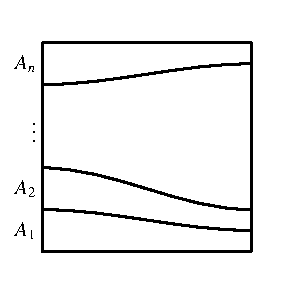
\includegraphics[width=0.3\hsize]{images/erwartung-4}
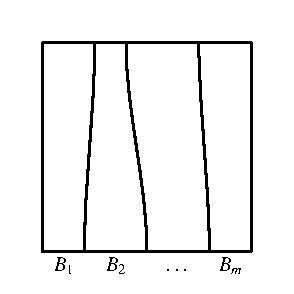
\includegraphics[width=0.3\hsize]{images/erwartung-3}
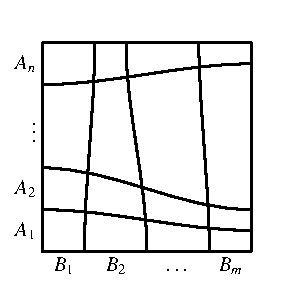
\includegraphics[width=0.3\hsize]{images/erwartung-2}
\end{center}
\caption{Ereignisse $A_i$ zur Berechung von $E(X)$, $B_j$ zur Berechnung
von $E(Y)$ und $A_i\cap B_j$ zur Berechnung von $E(XY)$.
\label{productexpectation}}
\end{figure}
Seien $A_i$ und $B_j$ Ereignisse so, dass $X$ auf den $A_i$ und $Y$ auf
den $B_j$ konstant ist. Dann kann man die Ereignisse $A_i\cap B_j$
zur Berechnung des Erwartungswertes heranziehen, wie in
Abbildung~\ref{productexpectation}, denn auf ihnen ist sowohl $X$ wie
auch $Y$ konstant.
Die Wahrscheinlichkeit von $A_i\cap B_j$ kann aber nur dann
durch die Wahrscheinlichkeiten von $A_i$ und $B_j$ ausgedr"uckt werden,
wenn die Ereignisse $A_i$ und $B_j$ paarweise
unabh"angig sind. Dann berechnet man:
\marginpar{\tiny\raggedright Rechenregel f"ur den Erwartungswert eines Produktes}
\begin{eqnarray*}
E(XY)&=&\sum_{i=1}^n\sum_{j=1}^m X(A_i\cap B_j)Y(A_i\cap B_j)P(A_i\cap B_j)\\
&=&\sum_{i=1}^n\sum_{j=1}^m X(A_i)Y(B_j)P(A_i)P(B_j)\\
&=&\sum_{i=1}^n X(A_i)P(A_i)\sum_{j=1}^mY(B_j)P(A_i)P(B_j)\\
&=&E(X)\cdot E(Y)
\end{eqnarray*}
Die oben verwendete Unabh"angigkeitsbedingung kann man mit folgender
Definition erzwingen:
\begin{definition}Zwei Zufallsvariable $X$ und $Y$ heissen
unabh"angig, wenn die Ereignisse $\{\omega|X(\omega)\le x\}$
und $\{\omega|Y(\omega)\le y\}$ f"ur alle $x,y\in\mathbb R$
unabh"angig sind, also
\[
P((X\le x)\wedge(Y\le y))=P(X\le x)\,P(Y\le y)\quad\forall x,y\in\mathbb{R}.
\]
\end{definition}
\index{Produktregel!f\"ur den Erwartungswert}
Damit haben wir auch f"ur Zufallsvariable eine Produktregel:
\begin{satz}
\label{produktregel-erwartungswert}
Sind $X$ und $Y$ unabh"angige Zufallsvariablen, dann gilt
\[
E(XY)=E(X)\cdot E(Y).
\]
F"ur zwei beliebige Funktionen $f$ und $g$ von $\mathbb{R}$ nach $\mathbb{R}$,
so dass $f(X)$ und $g(Y)$ immer noch Zufallsvariable sind, gilt
\[
E(f(X)g(Y))=E(f(X))E(g(Y)).
\]
\end{satz}
Seien $X$ und $Y$ die Augenzahlen beim W"urfeln mit zwei W"urfeln.
\marginpar{\tiny\raggedright Erwartungswert des Produktes der Augenzahlen
beim W"urfeln}
Die Ereignisse $X\le x$ und $Y\le y$ sind offensichtlich unabh"angig
(``horizontale und vertikale Streifen''), daher gilt
\[
E(XY)=E(X)E(Y)=3.5^2=12.25.
\]

\subsection{Erwartungswert und Integration}
\index{Erwartungswert!und Integration}
Die Berechnung des Erwartungswertes war im vorangegangene Abschnitt
einfach m"oglich, weil wir annehmen konnten, dass es Ereignisse $A$
gibt, auf denen die Zufallsvariable $X$ konstant ist. Wenn diese
Bedingung nicht mehr gilt, k"onnte man versuchen, den Erwartungswert
durch die Summe der kleinsten und gr"ossten m"oglichen Werte auf jedem
Ereignis $A_i$ einzuschachteln:
\[
\sum_{i=0}^nP(A_i)\min_{\omega\in A_i}X(\omega)
\le E(X)\le
\sum_{i=0}^nP(A_i)\max_{\omega\in A_i}X(\omega).
\]
Wir betrachten als Spezialfall die Ereignisalgebra f"ur eine
Messung, hier ist $\Omega=\mathbb{R}$. Die Wahrscheinlichkeitsfunktion $P$
liefert zu jedem Teilintervall $I\subset \mathbb{R}$ eine Wahrscheinlichkeit.
Wir betrachten eine Zerlegung der reellen Achse in Teilintervalle $I_i$.
Zu einer Funktion $X\colon \mathbb{R}\to\mathbb{R}$ kann man jetzt den
Erwartungswert wie folgt berechnen:
\[
\sum_{i=0}^nP(I_i)\min_{x\in I_i}X(x)
\le E(X)\le
\sum_{i=0}^nP(I_i)\max_{x\in I_i}X(x).
\]
Diese Konstruktion ist aber aus der Analysis vertraut, auf diese
Art wurde das Integral konstruiert. Die Summenausdr"ucke sind sogenannte
Riemannsche Summen, der einzige Unterschied ist, dass nicht die L"ange des
Intervalls, sondern die Wahrscheinlichkeit $P(I_i)$ des Intervalls gemessen
wird. Der Erwartungswert ist also eine Art verallgemeinertes Integral,
wof"ur der Mathematiker auch 
\[
E(X)=\int_{\Omega}X(\omega)dP(\omega)
\]
schreibt. Da uns diese Betrachtungsweise keine wirklich praktikablen
M"oglichkeiten zur Berechnung von $E(X)$ bietet, verfolgen wir sie
hier nicht weiter, werden aber im n"achsten Kapitel eine verwandte
Technik kennen lernen, welche nur gew"ohnliche Integrale verwendet.

\section{Varianz\label{section-varianz}}
\index{Varianz}
Die Qualit"atskontrolle bei der Herstellung von Widerst"anden versucht
ein Mass daf"ur zu entwickeln, wie genau die produzierten Widerst"ande
den beabsichtigen Widerstandswert einhalten. 
Dazu werden der Produktion einige Widerst"ande entnommen und ihr Wert
nachgemessen. Den Erwartungswert des Widerstandswertes kann man mit
Hilfe des Mittelwertes absch"atzen, er sollte ungef"ahr mit dem Sollwert
"ubereinstimmen.
\marginpar{\tiny\raggedright Varianz als Mass f"ur Streuung}
Wie aber kann man die ``Streuung'' der Widerstandswerte
bewerten?

Als weiteres Beispiel betrachten wir die die Zufallsvariable $X$
``Messung einer Spannung''. Nicht jede Messung ergibt den gleichen Wert,
\marginpar{\tiny\raggedright Varianz als Mass f"ur Rauschen}
das Signal ist von einem Rauschen "uberlagert. Der Mittelwert der
Messwert entspricht gem"ass dem vorangegangenen Abschnitt dem Erwartungswert
$E(X)$. Wie aber soll das Ausmass des Rauschens gemessen werden?
Ein praktischer Ansatz besteht darin, nach der Energie zu fragen, die
in dem Rauschsignal steckt. Die Leistung einer Wechselspannung $U(t)$
an einem Widerstand $R$ ist ja
$\frac{U(t)^2}R$, d.h. die mittlere Leistung w"ahrend des Intervalls $[t_0,t_1]$ 
ist
\[
\frac1{t_1-t_0}\int_{t_0}^{t_1}\frac{U(t)^2}R\,dt.
\]
Stellen wir uns vor, dass die Spannungsmessung $X$ in regelm"assigen, kurzen
Zeitintervallen wiederholt wird, dann ist die mittlere Leistung
des Differenzsignal $X-E(X)$ also proportional Summe der Quadrate
der Werte $(X-E(X))^2$, oder
\[
E((X-E(X))^2).
\]

\subsection{Definition}
\index{Varianz!Definition}
Die Einf"uhrungsbespiele motivieren folgende Definition:
\begin{definition}
\marginpar{\tiny\raggedright Definition der Varianz}
Sei $X\colon\Omega\to\mathbb{R}$ eine Zufallsvariable, dann
heisst die durch $\operatorname{var}(X)^2=E((X-E(X))^2)$ definierte Gr"osse $\operatorname{var}(X)$ die
{\bf Varianz} von $X$. Es ist insbesondere
\[
\operatorname{var}(X)=E((X-E(X))^2)=E(X^2)-E(X)^2
\]
\end{definition}
Die letzte Gleichung kann man leicht nachrechnen:
\begin{eqnarray*}
\operatorname{var}(X)&=&E((X-E(X))^2)\\
&=&E(X^2-2XE(X)+E(X)^2)\\
&=&E(X^2)-2E(X)E(X)+E(X)^2\\
&=&E(X^2)-E(X)^2\\
\end{eqnarray*}

\begin{figure}
\begin{center}
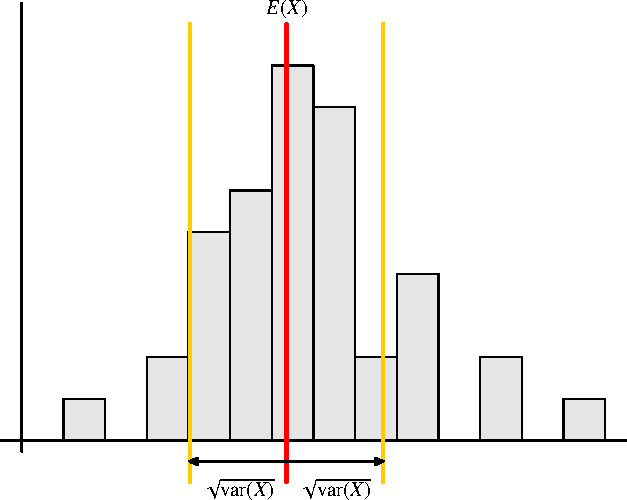
\includegraphics[width=\hsize]{images/erwartung-1}
\end{center}
\caption{Visualisierung von Erwartungswert und Varianz ein einem Histogramm
\label{histogram}}
\end{figure}

Man beachte, dass $\operatorname{var}(X)$ die Masseinheit des Quadrates
von $X$ hat.
Wenn also $X$ als Masseinheit eine L"ange hat,
dann hat $\operatorname{var}(X)$ die Masseinheit einer Fl"ache.
Insbesondere kann man $\operatorname{var}(X)$ nicht in der gleichen
Zeichnung visualisieren wie $E(X)$.
Aber die Gr"sse $\sqrt{\operatorname{var}(X)}$ hat die gleiche Masseinheit, sie
dr"uckt die ``Streubreite'' der Werte von $X$ aus,
wie in Abbildung~\ref{histogram} veranschaulicht.

Die Definition der Varianz ``passt'' in nat"urlicher Weise zum Erwartungswert,
wie der folgende Satz zeigt:
\begin{satz}\label{erwartungswert-charakterisierung}
\marginpar{\tiny\raggedright Minimumeigenschaft des Erwartungswertes}
Der Erwartungswert $E(X)$ einer reellen Zufallsvariable $X$ ist diejenige
reelle Zahl $\mu$, f"ur die $E((X-\mu)^2)$ minimal wird.
\end{satz}
\begin{proof}[Beweis]
Aus den Rechenregeln finden wir
\begin{eqnarray*}
E((X-\mu)^2)&=&E(X^2-2\mu X+\mu^2)\\
&=&E(X^2)-2\mu E(X) +\mu^2E(1)\\
&=&E(X^2)-2\mu E(X) +\mu^2P(\Omega)\\
&=&E(X^2)-2\mu E(X) +\mu^2
\end{eqnarray*}
Dies ist eine quadratische Funktion, die ihren Scheitelpunkt bei $\mu$ hat.
Man kann dies auch durch Nullsetzen der Ableitung nach $\mu$ finden:
\[
\frac{d}{d\mu}\left(E(X^2)-2\mu E(X) +\mu^2\right)=-2 E(X)+2\mu=0,
\]
Aufl"osen nach $\mu$ ergibt $\mu=E(X)$.
\end{proof}
Wir wenden die Definition der Varianz auf das Beispiel der Widerstandsmessung
an,
Wir haben bereits im Abschnitt \ref{erwartungswertvonmesswerten}
den Erwartungswert $E(R)=0.99015$ der Widerstandsmesswerte ermittelt, darauf aufbauend
k"onnen wir jetzt auch die Varianz berechnen.
Man findet zum Beispiel die Widerstandswerte gem"ass
Tabelle~\ref{varianzberechnung}.
\begin{table}
\begin{center}
\begin{tabular}{|c|r|r|r|}
\hline
Nummer&Messwert&Abweichung&$\text{Abweichung}^2$\\
\hline
1&0.990&-0.00015&0.0000000225\\
2&0.989&-0.00115&0.0000013225\\
3&0.991&0.00085&0.0000007225\\
4&0.991&0.00085&0.0000007225\\
5&0.991&0.00085&0.0000007225\\
6&0.989&-0.00115&0.0000013225\\
7&0.990&0.00015&0.0000000225\\
8&0.989&-0.00115&0.0000013225\\
9&0.992&0.00185&0.0000034225\\
10&0.992&0.00185&0.0000034225\\
11&0.990&-0.00015&0.0000000225\\
12&0.989&-0.00115&0.0000013225\\
13&0.990&-0.00015&0.0000000225\\
14&0.991&0.00085&0.0000007225\\
15&0.989&-0.00115&0.0000013225\\
16&0.990&-0.00015&0.0000000225\\
17&0.989&-0.00115&0.0000013225\\
18&0.990&-0.00015&0.0000000225\\
19&0.990&-0.00015&0.0000000225\\
20&0.991&0.00085&0.0000007225\\
\hline
&$\mu=1.000$&$\sigma=0.000963$&
$\sigma^2=0.0000009275$\\
\hline
\end{tabular}
\end{center}
\caption{Einzelmessungen an Widerst"anden und Berechnung der Varianz
\label{varianzberechnung}}
\end{table}

\subsubsection{Beispiel: Wurf einer fairen M"unze}
Beim Wurf einer fairen M"unze werde der Gewinn $1$ ausbezahlt bei
``Kopf'', bei ``Zahl'' wird hingegen $0$ ausbezahlt. Es ist klar,
dass die erwartete Auszahlung $E(X)=\frac12$ ist.
Daraus l"asst sich jetzt auch die Varianz berechnen:
\begin{align*}
\operatorname{var}(X)
&=
E((X-E(X))^2)=E\biggl(\biggl(X-\frac12\biggr)^2\biggr)
=\frac12\cdot \biggl(1-\frac12\biggr)^2+\frac12\biggl(0-\frac12\biggr)^2\\
&=\frac12\cdot\frac14+\frac12\cdot\frac14=\frac14.
\end{align*}

\subsection{Empirische Berechnung}
\index{Varianz!angen\"aherte Berechnung}
Wir betrachten das praktische Beispiel der Bestimmung der Varianz
\marginpar{\tiny\raggedright Berechnung der Varianz}
einer Messreihe.
Gegeben sind also die Messwerte $(x_i)_{1\le i\le n}$
Auf den ersten Blick sieht es so aus, als w"are f"ur die Berechnung der Varianz
sehr viel Speicherplatz erforderlich. Zwar ist f"ur die Berechnung des
Erwartungswertes von $\mu=E(X)=\frac1n\sum_{i=1}^n x_i$ kein besonderer Aufwand
notwendig, da die Summe laufend gebildet werden kann. Zur Berechnung der
Varianz muss aber erst $\mu$ bestimmt werden, bevor man die Differenzen $(x_i-\mu)$
bilden kann. Trotzdem l"asst sich die Berechnung vereinfachen:
\begin{eqnarray*}
E((X-\mu)^2)&=&\frac1n\sum_{i=1}^n(x_i-\mu)^2\\
&=&\frac1n\sum_{i=1}^n(x_i^2-2\mu x_i+\mu^2)\\
&=&\frac1n\sum_{i=1}^nx_i^2-2\mu\frac1n\sum_{i=1}^n x_i+\mu^2\\
&=&\frac1n\sum_{i=1}^nx_i^2-\bigl(\frac1n\sum_{i=1}^nx_i\bigr)^2\\
\end{eqnarray*}
\subsubsection{Beobachtungen}
\begin{enumerate}
\item
Es gen"ugt also, $x_i$ und $x_i^2$ zu summieren, wozu nur zwei Speicherpl"atze
ben"otigt werden.
Aus den beiden Summen kann die Varianz bereits berechnet werden.
Es ist nicht n"otig, die einzelnen Messwerte $x_i$ zu speichern.
\item
Die Berechnung der Varianz kann also ganz einfach mit einer Tabelle
erfolgen:
\begin{center}
%\begin{tabular}{|>{$}c<{$}|>{$}c<{$}|}
\begin{tabular}{|c|c|c|}
\hline
$i$&$x_i$&$x_i^2$\\
\hline
$1$&$x_1$&$x_1^2$\\
$2$&$x_2$&$x_2^2$\\
$\vdots$&$\vdots$&$\vdots$\\
$n$&$x_n$&$x_n^2$\\
\hline
&$\sum_{k=0}^n x_i$&$\sum_{k=0}^n x_i^2$\\
\hline
\end{tabular}
\end{center}
\item
Grosse Abweichungen k"onnen vorkommen, und bekommen wegen des
Quadrates in der Varianz auch grosses Gewicht. Hat man aber nur
wenige Messwerte, ist es unwahrscheinlich, eine solche grosse
Abweichung, einen ``Ausreisser'', zu sehen. Daher untersch"atzt
diese empirische Formel den tats"achlichen Wert der Varianz immer
dann, wenn $n$ klein ist. Wir werden sp"ater sehen, dass eine
besser Sch"atzung zu bekommen ist, wenn man noch einen Korrekturfaktor
$\frac{n}{n-1}$ hinzuf"ugt.
\end{enumerate}

\subsection{Weitere Rechenregeln}
\begin{satz}
\label{rechenregeln-varianz}
Seien $X$ und $Y$ unabh"angige Zufallsvariable, dann haben
Summe und Produkt folgende Varianz:
\begin{eqnarray*}
\operatorname{var}(\lambda X)&=&\lambda^2\operatorname{var}(X)\\
\operatorname{var}(X+Y)&=&\operatorname{var}(X)+\operatorname{var}(Y)\\
\operatorname{var}(XY)&=&\operatorname{var}(X)\operatorname{var}(Y)
+
\operatorname{var}(Y)E(X)^2+\operatorname{var}(X)E(Y)^2
\end{eqnarray*}
\end{satz}
\begin{proof}[Beweis]Durch einfaches Nachrechnen unter Ausn"utzen der
Rechenregeln f"ur den Erwartungswert und der
Unabh"angigkeit von $X$ und $Y$, d.h. $E(XY)=E(X)E(Y)$:
\begin{eqnarray*}
\operatorname{var}(X+Y)
&=&E((X+Y)^2)-E(X+Y)^2\\
&=&E(X^2+2XY+Y^2)-(E(X)+E(Y))^2\\
&=&E(X^2)+2E(XY)+E(Y^2)-E(X)^2-2E(X)E(Y)-E(Y)^2\\
&=&E(X^2)-E(X)^2+E(Y^2)-E(Y)^2\\
&=&\operatorname{var}(X)+\operatorname{var}(Y)
\end{eqnarray*}
Durch ziehen der Wurzel folgt die Behauptung aus der letzten Gleichung.
F"ur das Produkt gilt
\begin{eqnarray*}
\operatorname{var}(XY)
&=&E(X^2Y^2)-E(XY)^2\\
&=&E(X^2)E(Y^2)-E(X)^2E(Y)^2\\
&=&(\operatorname{var}(X)+E(X)^2))(\operatorname{var}(Y)+E(Y)^2)
-E(X)^2E(Y)^2\\
&=&\operatorname{var}(X)\operatorname{var}(Y)+E(X)^2\operatorname{var}(Y)
+\operatorname{var}(X)E(Y)^2
\end{eqnarray*}
und daraus die Behauptung.
\end{proof}

\subsubsection{Beobachtungen}

\begin{enumerate}
\item
Die Varianz funktioniert "ahnlich wie das Quadrieren f"ur gew"ohnliche Zahlen.
Schreibt man $E(XY)-E(X)E(Y)=\operatorname{cov}(X,Y)$, lautete die
binomische Formel wird f"ur die Varianz:
\begin{equation}
\operatorname{var}(X+Y)=\operatorname{var}(X)
+2\operatorname{cov}(X,Y)
+\operatorname{var}(Y).
\label{var-summe-abhaengig}
\end{equation}
Die Kovarianz $\operatorname{cov}(X,Y)$ spielt also die Rolle des gemischten
Terms in der ``ge"ohnliche'' binomischen Formel.
\item
Sind $X$ und $Y$ unabh"angig, gilt daher die Formel
\begin{align*}
\operatorname{var}(X+Y)
&=
\operatorname{var}(X)
+
\operatorname{var}(Y)
\\
\sqrt{\operatorname{var}(X+Y)}
&=
\sqrt{
\sqrt{\operatorname{var}(X)}^2
+
\sqrt{\operatorname{var}(Y)}^2
}
\end{align*}
Die Gr"ossen $\sqrt{\operatorname{var}(X)}$ und $\sqrt{\operatorname{var}(Y)}$
werden daher wie die Katheten eines rechtwinkligen Dreiecks addiert,
man spricht von {\it pythator"aischer} Addition.
\end{enumerate}

\subsubsection{Anwendung: Wurf von $n$ M"unzen}
Sei $X$ die Anzahl ``Kopf'' beim Wurf von $n$ M"unzen. Nat"urlich wird
$X$ nur Werte zwischen $0$ und $n$ annehmen.
Zur Berechnung von $E(X)$ und $\operatorname{var}(X)$ wollen wir
die Rechenregeln verwenden. Dabei verwenden wir neue Zufallsvariablen
$X_i$ wie folgt:
\begin{center}
\begin{tabular}{clcc}
$X_1$&Anzahl Kopf im ersten Wurf&$E(X_1)=\frac12$&$\operatorname{var}(X_1)=\frac14$\\
$X_2$&Anzahl Kopf im zweiten Wurf&$E(X_2)=\frac12$&$\operatorname{var}(X_2)=\frac14$\\
&$\dots$&&\\
$X_n$&Anzahl Kopf im $n$-ten Wurf&$E(X_n)=\frac12$&$\operatorname{var}(X_n)=\frac14$\\
\end{tabular}
\end{center}
Damit kann man Erwartungswert und Varianz von $X=X_1+X_2+\dots+X_n$ berechnen:
\begin{align*}
E(X)&=
E(X_1)+
E(X_2)+\dots+
E(X_n)
=
\frac{1}2+
\frac{1}2+\dots+
\frac{1}2=\frac{n}2
\\
\operatorname{var}(X)
&=
\operatorname{var}(X_1)
+
\operatorname{var}(X_2)
+\dots+
\operatorname{var}(X_n)
=\frac14+\frac14+\dots+\frac14=\frac{n}4.
\end{align*}

\section{Wie genau ist der Mittelwert?}
Der Erwartungswert dr"uckt aus, wie gross eine Zufallvariable ``im Mittel''
sein wird.
Je gr"osser aber die Varianz ist, desto gr"osser wird die Abweichung
der Zufallsvariable vom ``mittleren Wert'' sein.
Wie misst man diese Abweichung? Mit der Varianz haben wir bereits
ein Mass f"ur die mittlere Abweichung, aber noch keinen Hinweis
darauf, wie h"aufig grosse Abweichungen vorkommen werden.

Sei $\mu=E(X)$ der Erwartungswert der Zufallsvariablen $X$.
F"ur die Varianz hatten wir die Abweichung $X-\mu$ der Zufallsvariablen
von ihrem Erwartungswert untersucht.
Meistens wird die Abweichung klein sein. Uns interessiert jetzt aber,
wie wahrscheinlich es ist, dass sie gross ist.
Sei $\varepsilon>0$ ein Schwellwert f"ur die Abweichung, wir m"ochten
also wissen, wie h"aufig die Abweichung $\varepsilon$ "uberschreitete:
\[
|X-\mu|>\varepsilon.
\]
Wir m"ochten die Wahrscheinlichkeit 
\[
P(|X-\mu|>\varepsilon)
\]
berechnen.
Nach unseren einleitenden Bemerkungen sollte es einen Zusammenhang
zwischen Varianz und und dieser Wahrscheinlichkeit geben: je gr"osser
die Varianz, desto gr"osser die Wahrscheinlichkeit einer grossen
Abweichung.

\subsection{Ungleichung von Tschebyscheff}\label{ungleichung-von-tschebyscheff}
\index{Tschebyscheff!Ungleichung von}
Selbst wenn man gar nichts "uber die Zufallsvariable weiss, ausser
dass sie eine Varianz besitzt, kann man eine Aussage "uber die 
Wahrscheinlichkeit einer grossen Abweichung machen.
Dies ist der Inhalt der Ungleichung von Tschebyscheff.
Dies kann nat"urlich
nur eine grobe obere Schranke sein, f"ur genaue Resultate muss man
mehr "uber das konkrete Experiment wissen.
\marginpar{\tiny\raggedright Wahrscheinlichkeit f"ur Abweichung vom Erwartungswert}

\begin{satz}[Ungleichung von Tschebyscheff]
Ist eine Zufallsvariable $X$, dann l"asst sich die Wahrscheinlichkeit,
dass $X$ um mehr als $\varepsilon$ vom Erwartungswert abweicht, wie
folgt absch"atzen:
\[
P(|X-\mu| >\varepsilon)\le\frac{\operatorname{var}(X)}{\varepsilon^2}
\]
\end{satz}

L"asst man $\varepsilon$ wachsen findet man, dass Abweichungen
deutlich gr"osser als $\sqrt{\operatorname{var}(X)}$ 
sehr unwahrscheinlich sind.

\begin{proof}[Beweis]
Sei $A =\{\omega\;|\;|X(\omega)-\mu|>\varepsilon\}$ das Ereignis, dass die
Zufallsvariable $X$ um mehr als $\varepsilon$ vom Mittelwert abgewichen
ist. Offensichtlich ist dies dasselbe, wie wenn $(X-\mu)^2$ mehr als
$\varepsilon^2$ von 0 abweicht. Es gilt daher:
\[
\varepsilon^2 \chi_{A} \le (X-\mu)^2
\]
Wenden wir darauf den Erwartungswert an, folgt
\[
\varepsilon^2 P(A)\le E((X-\mu)^2)=\operatorname{var}(X)
\]
Die Tschebyscheffsche Ungleichung folgt jetzt nach Division durch
$\varepsilon^2$.
\end{proof}
Beispiel:
\marginpar{\tiny\raggedright Anwendung: Produktions"uberwachung}
Bei der Herstellung von 1k$\Omega$ Widerst"anden
m"ochte man sicherstellen,
dass nur bei 1\% aller produzierten Widerst"ande der Wert um mehr als
10$\Omega$ vom Sollwert abweicht. Um das zu "uberpr"ufen entnimmt man der
Produktion eine Stichprobe, und sch"atzt die Varianz ab. Wie gross darf die
Varianz maximal werden, damit die Bedingung noch erf"ullt ist?

Die Tschebyscheffsche Ungleichung liefert in diesem Fall
\[
\operatorname{var}(X)\ge\varepsilon^2P(|X-\mu| >\varepsilon)
\]
oder
\[
\operatorname{var}(X)\ge 10^2\cdot 0.01=1.
\]
Sobald die Varianz der Stichprobe gr"osser als 1$\Omega^2$ ist, kann die
Tschebyscheffungleichung die Einhaltung der Qualit"atsvorgabe nicht
mehr garantieren.

Die Tschebyscheff-Ungleichung ist bei weitem nicht die bestm"ogliche.
\marginpar{\tiny\raggedright Grenzen der Tschebyscheff-Ungleichung}
Fragt man zum Beispiel nach der Wahrscheinlichkeit, dass $X$ um mehr
als zwei Standardabweichungen, also um mehr als $2\sqrt{\operatorname{var}(X)}$ vom
Erwartungswert abweicht, dann liefert sie
\[
P(|X-\mu|>2\sqrt{\operatorname{var}(X)})
\le\frac{\operatorname{var}(X)}{2^2\operatorname{var}(X)}=\frac14.
\]
Diese Ungleichung gilt f"ur jede Zufallsvariable $X$.
Es gibt aber Zufallsvariablen, f"ur die 
\[
P(|X-\mu|>2\sqrt{\operatorname{var}(X)})\le 0.05,
\]
Wir werden mit der Normalverteilung solche Zufallsvariablen kennenlernen.
Auf das Beispiel angewendet bedeutet dies, dass die Tschebyscheff-Ungleichung
m"oglicherweise viel zu oft behauptet, dass die Produktionsqualit"at ungen"ugend
ist, weil die Widerstandswerte vermutlich in guter N"aherung normalverteilt
sein werden.

\subsection{Wie gut approximiert der Mittelwert den Erwartungswert?}
\label{approximation-mittelwert}
Wir betrachten eine Folge von unabh"angigen Zufallsvariablen $X_1, X_2,\dots$, die
alle den gleichen Erwartungswert $E(X_i)=\mu$ und die gleiche Varianz
$\operatorname{var}(X_i)=\sigma^2$ haben. Dann erwartet man, dass 
der Mittelwert der ersten $n$ Zufallsvariablen, also die
\marginpar{\tiny\raggedright Mittelwert von Zufallsvariablen}
Gr"osse
\[
M_n=\frac{X_1+X_2+\dots+X_n}{n}
\]
eine gut N"aherung ist f"ur $\mu$. Trotzdem kann es vorkommen, wegen
einzelner Ausreisser unter den $X_i$ der Mittelwert recht weit weg
vom Mittelwert liegt. Der folgende Satz von Bernoulli sagt, wie wahrscheinlich
es ist, dass der Mittelwert weiter als $\varepsilon$ vom Erwartungswert
entfernt ist.

Zun"achst halten wir fest, dass
\[
M_n=\frac{X_1+\dots+X_n}{n}
\]
eine Zufallsvariable ist mit Erwartungswert
\[
E(M_n)=E\biggl(\frac{X_1+\dots+X_n}{n}\biggr)
=\frac{E(X_1)+\dots+E(X_n)}{n}=\mu
\]
und Varianz
\[
\operatorname{var}(M_n) =\frac1{n^2}\sum_{i=1}^n\operatorname{var}(X_i)
=\frac{\sigma^2}n,
\]
wie man mit den Rechenregeln f"ur die Varianz sofort nachrechnet.

\index{Gesetz der grossen Zahlen}
\index{Bernoulli!Gesetz der grossen Zahlen}
\begin{satz}[Bernoullis Gesetz der grossen Zahlen]
Die Wahrscheinlichkeit, dass der Mittelwert von $n$ unabh"angigen Zufallsvariablen
mit Mittelwert $\mu$ und Varianz $\sigma^2$ mehr als $\varepsilon$ von $\mu$
abweicht ist
\[
P(|M_n-\mu|>\varepsilon)\le \frac{\sigma^2}{\varepsilon^2n}.
\]
Insbesondere gilt
\[
\lim_{n\to\infty}P(|M_n-\mu|>\varepsilon)=0.
\]
\end{satz}
\begin{proof}[Beweis]
Aus der Tschebyscheffschen Ungleichung folgt:
\[
P(|M_n-\mu|>\varepsilon)\le\frac{\operatorname{var}(M_n)}{\varepsilon^2}=
\frac{\sigma^2}{n\varepsilon^2}.
\]
Dies entspricht genau der Behauptung.
\end{proof}
Leider sind die Vorhersagen wie auch bei der Tschebyscheff-Ungleichung
nur beschr"ankt n"utzlich. Wenn die Wahrscheinlichkeit, dass der Mittelwert
um mehr als $\sigma$ vom Erwartungswert abweicht, kleiner als 1\% sein
soll, sind daf"ur nach dem Gesetz der grossen Zahlen mindestens 100 Summanden
n"otig.

\subsection{Wie genau ist die empirische H"aufigkeit?}
Wir haben durch Wiederholung von Experimenten auch versucht, die
Wahrscheinlichkeit eines Ereignisses durch die H"aufigkeit zu approximieren,
mit welcher dieses Ereignis eintritt.
Mit dem Satz von Bernoulli ist es uns jetzt auch m"oglich, die
Wahrscheinlichkeit daf"ur abzusch"atzen, dass wir ein falsches
Resultat erhalten.
\begin{satz}
Wird ein Experiment $n$ mal durchgef"uhrt, und tritt dabei das Ereignis $A$
mit der relativen H"aufigkeit $h$ ein, dann ist die Wahrscheinlichkeit,
dass $h$ um mehr als $\varepsilon$ von $P(A)$ abweicht
\[
P(|h- P(A)|>\varepsilon)\le \frac{P(A)(1-P(A))}{n\varepsilon^2}
\le\frac{1}{4n\varepsilon^2}
\]
\end{satz}
\begin{proof}[Beweis]
Wir betrachten die Zufallsvariablen $X_i$, welche den Wert $1$ hat,
wenn im $i$-ten Versuch das Ereignis $A$ eingetreten ist, und sonst $0$.
Diese Zufallsvariablen sind offensichtlich unabh"angig. Betrachtet man
nur die einzelne Durchf"uhrung $i$ des Versuches, dann ist $X_i$
die Funktion
$\chi_A$, welchen
den Erwartungswert $E(\chi_A)=P(A)$, und die Varianz ist
\begin{eqnarray*}
\operatorname{var}(\chi_A)&=&E(\chi_A^2)-E(\chi_A)^2=E(\chi_A)-E(\chi_A)^2\\
&=&P(A)-P(A)^2=P(A)(1-P(A))
\end{eqnarray*}
hat.
Der Mittelwert $M_n$ ist die Anzahl der Versuche, bei denen das Ereignis
$A$ eingetreten ist, geteilt durch $n$, also die Anzahl aller Versuche,
$h=M_n$. Damit folgt aus dem Gesetz der grossen Zahlen:
\[
P(|h-P(A)|>\varepsilon)\le\frac{P(A)(1-P(A))}{n\varepsilon^2}.
\]
Die letzte Ungleichung des Satzes folgt aus der Tatsache, dass die Funktion
$p\mapsto p(1-p)=p-p^2$ bei $p=\frac12$ ein Maximum hat, also
$P(A)(1-P(A))\le\frac14$ gilt.
\end{proof}
Insbesondere verstehen wir jetzt, warum es sehr lange dauern kann, bis
wir durch Z"ahlen der H"aufigkeit eines Ereignisses dessen Wahrscheinlichkeit
auch nur auf wenige Stellen nach dem Komma bestimmen k"onnen. Wenn wir
verlangen, dass die relative H"aufigkeit mit
99\% Sicherheit die Wahrscheinlichkeit auf drei Stellen ann"ahert, also
$\varepsilon=10^{-3}$, dann m"ussen wir verlangen
\begin{eqnarray*}
\frac{1}{4n\varepsilon^2}&\le&0.01\\
\frac1{4\cdot 10^{-3\cdot 2}\cdot10^{-2}}=25\cdot 10^6&\le&n.
\end{eqnarray*}
Der Versuch muss also mindestens 25 Millionen mal wiederholt werden,
um eine Genauigkeit von drei Stellen nach dem Komma mit 99\% Sicherheit
zu erreichen. Dies deckt sich mit den Beobachtungen in der W"urfelsimulation
in Tabelle
\ref{wuerfel-simulation}.
\section{Lineare Regression}
\index{Regression!lineare}
\index{lineare Regression}
\index{Kurvenanpassung}
\begin{figure}
\begin{center}
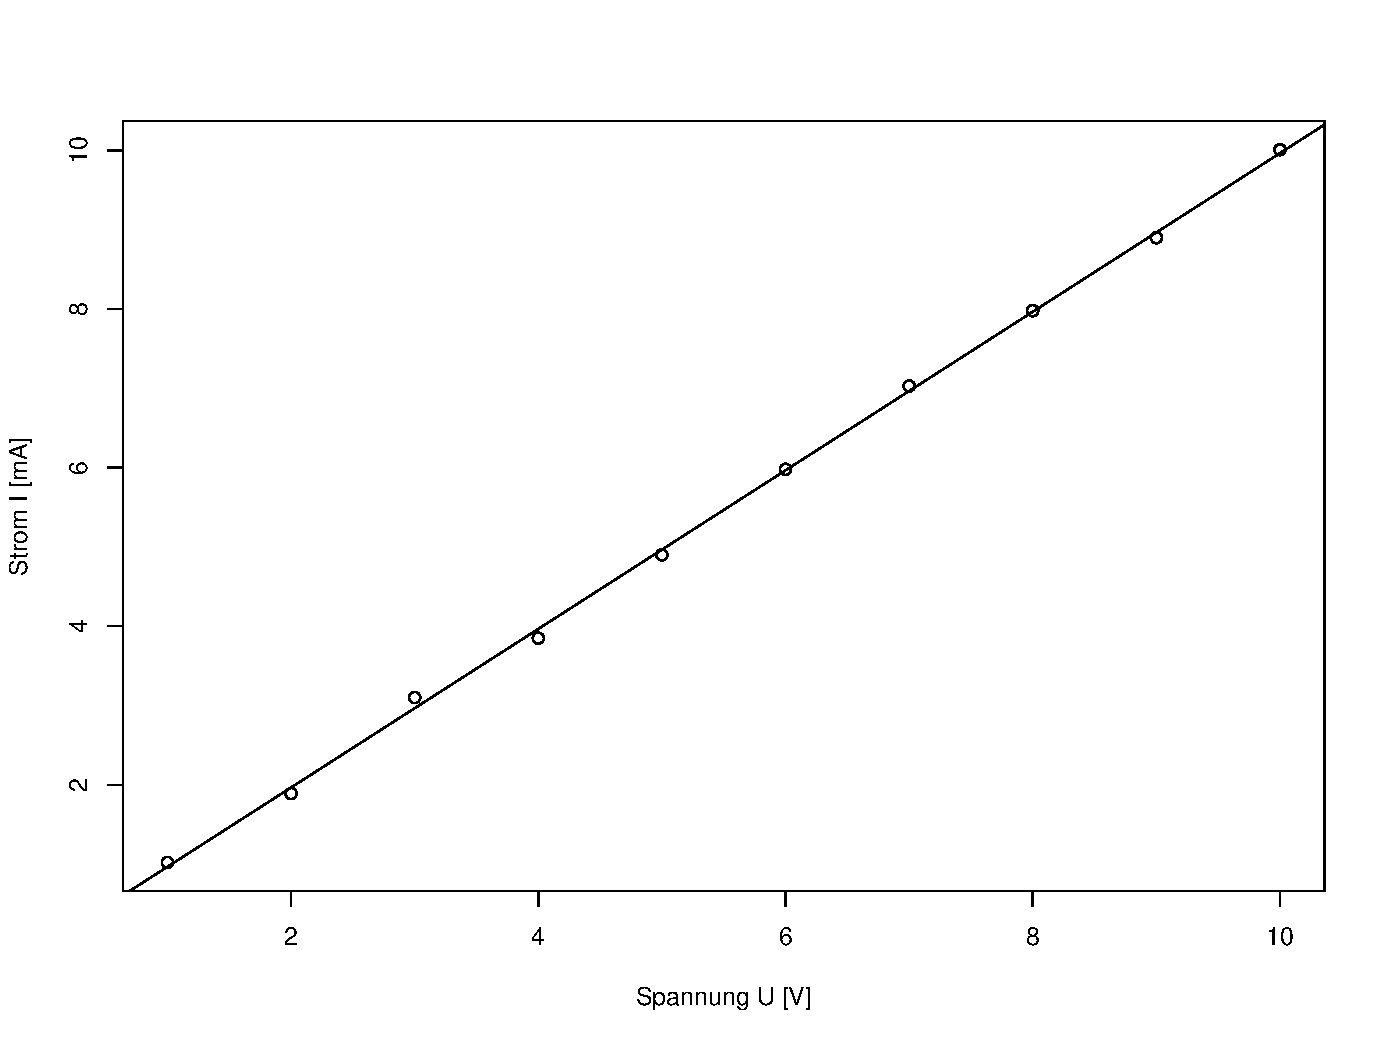
\includegraphics[width=0.8\hsize]{graphics/ohm}
\end{center}
\caption{Anpassung einer Geraden an gemessen Strom-/Spannungs-Werte\label{ohm-regression}}
\end{figure}
Der Satz \ref{erwartungswert-charakterisierung} hat gezeigt, dass der
Erwartungswert jener Wert ist, der die Varianz minimiert. Diese Idee
l"asst sich auch auf kompliziertere Zusammenh"ange anwenden. In einem
Stromkreis erwartet man auf Grund des Ohmschen Gesetzes, dass Spannung $U$
und Strom $I$ proportional sind: $U=RI$. F"uhrt man eine Messung von beiden
Gr"ossen durch, erh"alt man zwei Zufallsvariablen $U(\omega)$ und $I(\omega)$,
und die Proportionalit"at wird wegen der Messfehler meistens nicht mehr
erf"ullt sein. Wie gross ist der Widerstansdwert $R$? Es w"are zwar denkbar,
f"ur jede Messung den Widerstandswert zu errechnen, und dann das Mittel
zu bilden. Noch besser ist aber, den Widerstandswert $R$ so zu bestimmen,
dass der erwartete quadratische Fehler
$E( (U-RI)^2)$
m"oglichst klein ist.
\marginpar{\tiny\raggedright Regressionsgerade als lineare N"aherung f"ur einen Datensatz}
Abbildung \ref{ohm-regression} zeigt eine solche Gerade.


\subsection{Regressionsgerade}
Etwas allgemeiner finden wir folgenden Satz "uber die sogenannte
Regressionsgerade:
\begin{satz}
\label{rekursion}
Seien $X$ und $Y$ zwei reelle Zufallsvariable. Die Gerade mit der
Gleichung $y=ax+b$ minimiert die Varianz
$\operatorname{var}(aX+b-Y)$ genau dann, wenn 
\begin{eqnarray*}
a&=&\frac{E(XY)-E(X)E(Y)}{(E(X^2)-E(X)^2)}=\frac{\operatorname{cov}(X,Y)}{\operatorname{var}(X)}\\
b&=&E(Y)-E(X)a
\end{eqnarray*}
\end{satz}
\begin{proof}[Beweis]
Der mittlere quadratische Fehler ist
\begin{eqnarray*}
Q(a,b)&=&E((aX+b-Y)^2)\\
&=&E(a^2X^2+b^2+Y^2+2abX-2aXY -2bY)\\
&=&a^2E(X^2)+b^2+E(Y^2)+2abE(X)-2aE(XY)-2bE(Y)
\end{eqnarray*}
Um das Minimum zu finden, setzen wir die partiellen Ableitungen nach $a$
und $b$ gleich Null, und finden:
\begin{eqnarray*}
0=\frac{\partial Q}{\partial a}&=&2aE(X^2)+2bE(X)-2E(XY)\\
0=\frac{\partial Q}{\partial b}&=&2b+2aE(X)-2E(Y)\\
\end{eqnarray*}
Dies ist gleichbedeutend mit dem folgenden linearen Gleichungssystem f"ur
die Koeffizienten
$a$ und $b$
\begin{alignat*}{4}
E(X^2)a\,&+\,&E(X)b\,&=\,&E(XY)\\
E(X)a\,&+&b\,&=&E(Y)
\end{alignat*}
Multipliziert man die zweite Gleichung mit $E(X)$ und subtrahiert sie von der
ersten, erh"alt man eine Gleichung f"ur $a$:
\begin{eqnarray*}
(E(X^2)-E(X)^2)a&=&E(XY)-E(X)E(Y)\\
a&=&\frac{E(XY)-E(X)E(Y)}{(E(X^2)-E(X)^2)} 
\end{eqnarray*}
Aus der zweiten Gleichung kann man nun auch $b$ finden:
\[
b=E(Y)-E(X)a
\]
womit alles bewiesen ist.
\end{proof}
Die Gleichung f"ur $b$ hat eine unmittelbare Konsequenz: die Regressionsgerade
geht immer durch den Punkt $(E(X), E(Y))$. In der Tat, damit der Punkt
$(E(X), E(Y))$ auf der Geraden liegt, muss die Bedinung $E(Y)=aE(X)+b$
erf"ullt sein. Schafft man $aE(X)$ auf die linke Seite, wird daraus
$E(Y)-aE(X)=b$, also genau die Gleichung f"ur $b$.

\subsubsection{Der mittlere quadratische Fehler}
Der mittlere quadratische Fehler l"asst sich nat"urlich auch berechnen.
Wir sind von $\operatorname{var}(Y-aX-b)$ als zu optimierender
Gr"osse ausgegangen. Inzwischen haben wir $a$ und $b$ bestimmt,
also k"onnen wir auch den Fehler berechnen. Dazu sind die Rechenregeln
hilfreich:
\begin{align*}
\operatorname{var}(Y-aX-b)
&=
\operatorname{var}(Y) + 
\operatorname{var}(-aX) + 
\operatorname{var}(-b)
+2\operatorname{cov}(-aX,Y)
\\
&=
\operatorname{var}(Y)+a^2\operatorname{var}(X)-2a\operatorname{cov}(X,Y)
\\
&=
\operatorname{var}(Y)
+ \frac{\operatorname{cov}(X,Y)^2}{\operatorname{var}(X)^2}\operatorname{var}(X)
-2 \frac{\operatorname{cov}(X,Y)}{\operatorname{var}(X)}\operatorname{cov}(X,Y)
\\
&=
\operatorname{var}(Y)-\frac{\operatorname{cov}(X,Y)^2}{\operatorname{var}(X)}
\end{align*}
Im zweiten Schritt mussten wir die Formel (\ref{var-summe-abhaengig})
verwenden, da die Zufallsvariablen $X$ und $Y$ nicht unabh"angig sind.

Nat"urlich
ist der Fehler 
wahrscheinlich ungef"ahr proportional zur Varianz der $Y$-Werte,
ohne Varianz gibt's auch keinen Fehler. Wir versuchen daher den Term
$\operatorname{var}(Y)$ auszuklammern:
\begin{align*}
\operatorname{var}(Y-aX-b)
&=
\operatorname{var}(Y)\left(1-\frac{\operatorname{cov}(X,Y)^2}{\operatorname{var}(X)\operatorname{var}(Y)}\right).
\end{align*}
Der Bruch wird damit ein nat"urliches Qualit"atsmass f"ur die Regressionsgerade:
\begin{definition}
\marginpar{\tiny\raggedright Definition des Regressionskoeffizienten}
Der Quotient
\[
r=\frac{\operatorname{cov}(X,Y)}{\sqrt{\operatorname{var}(X)\operatorname{var}(Y)}}
\]
heisst Regressionskoeffizient.
\end{definition}

Die Regression ist also umso genauer, je n"aher $r$ bei $\pm 1$ liegt.
Ausserdem hat $r$ immer das gleiche Vorzeichen wie die
Steigung der Regressionsgeraden.

\subsubsection{Berechnung aus empirischen Daten}
Auch die Koeffizienten der Regressionsgeraden sind mit einfachen Formeln
\marginpar{\tiny\raggedright Regressions-Formeln f"ur endliche Messreihen}
zu bestimmen, wenn man nur Messwerte, deren Quadrate und das Produkt summiert:
\begin{eqnarray*}
a&=&\frac{\displaystyle n\sum_{i=1}^nx_iy_i-\sum_{i=1}^nx_i\sum_{i=1}^ny_i}{\displaystyle n\sum_{i=1}^nx_i^2-\biggl(\sum_{i=1}^nx_i\biggr)^2}\\
b&=&\frac1n\sum_{i=1}^ny_i-a\frac1n\sum_{i=1}^nx_i\\
\end{eqnarray*}

\subsection{Anwendungsbeispiel}
\begin{table}
\begin{center}
\begin{tabular}{|c|c|}
\hline
Zeit [s]&L"ange [mm]\\
\hline
6&10.98\\
10&13.89\\
14&16.23\\
18&18.57\\
\hline
\end{tabular}
\end{center}
\caption{L"ange der Verz"ogerungselemente f"ur K1100T in Abh"angigkeit von der
Verz"ogerungszeit\label{delaylengths}}
\end{table}
Modellraketenmotoren auf Feststoffbasis verwenden ein Verz"ogerungselement,
welches nach Abbrand das eigentlichen Treibsstoffs noch einige Sekunden
weiter brennt, um dann eine Schwarzpulverladung zu z"unden, die einen Fallschirm
auswerfen kann. Die Verz"ogerungselemente werden nur f"ur wenige, diskrete
Verz"ogerungszeiten hergestellt. Ist kein passendes Verz"ogerungselement
verf"ugbar, muss
ein l"angeres Verz"ogerungselement durch Verk"urzung auf die passende
Verz"ogerungszeit eingestellt werden. Dazu muss jedoch der Zusammenhang
zwischen Verz"ogerungszeit und l"ange des Elementes bekannt sein.
Der Hersteller macht die Angaben in Tabelle \ref{delaylengths}.

\subsubsection{Berechnung von Hand}
Die Berechnung auf dem Papier kann man zum Beispiel mit Hilfe
\marginpar{\tiny\raggedright Berechnungsschema f"ur Regression von Hand}
des Berechnungsschemas gem"ass folgender Tabelle
organisieren, welche auch alle relevanten Formeln zeigt:
\begin{center}
\begin{tabular}{|l|l|l|l|}
\hline
$E(T)$&&&\\
$E(T^2)$&\footnotesize$\operatorname{var}(T)=E(T^2)-E(T)^2$&&\\
\hline
$E(L)$&&&\\
$E(L^2)$&\footnotesize$\operatorname{var}(L)=E(L^2)-E(L)^2$&&\\
\hline
$E(TL)$&\footnotesize$\operatorname{cov}(T,L)=E(TL)-E(T)E(L)$&$a=\frac{\operatorname{cov}(T,L)}{\operatorname{var}(T)}$&\footnotesize$b=E(L)-aE(T)$\\
&&$r=\frac{\operatorname{cov}(T,L)}{\sqrt{\operatorname{var}(T)\operatorname{var}(L)}}$&\\
\hline
\end{tabular}
\end{center}
Die Durchf"uhrung der Rechnung f"uhrt zu folgendem Resultat:
\begin{center}
\begin{tabular}{|r|r|r|r|}
\hline
12.0000&&&\\
164.0000&20.0000&&\\
\hline
14.9175&&&\\
230.4376&7.9058&&\\
\hline
191.5650&12.5550&0.627750&7.38450\\
&&0.998456&\\
\hline
\end{tabular}
\end{center}
Somit kann man als N"aherungsformel f"ur die L"ange des Verz"ogerungselements
die lineare Funktion
\[
l=0.62775 \cdot t+7.3845
\]
verwenden. Der mittlere quadratische Fehler dieser N"aherung ist
\[
\Delta = \operatorname{var}(L)(1-r^2)=0.024.
\]
Der L"angenfehler ist also etwa $\sigma_L=\sqrt{0.024}=0.15$mm, was einer
Ungenauigkeit der Verz"ogerungsdauer von 0.25s entspricht. Angesichts
der Fertigungs- und Betriebs\-toleranzen von bis zu 20\%, verursacht durch
Schwankungen in Abmessungen, physikalischen Eigenschaften des Treibstoffs
und Temperatur beim Abbrand ist dies bei weitem genau genug.
\subsubsection{Berechnung mit R}
\begin{figure}
\begin{center}
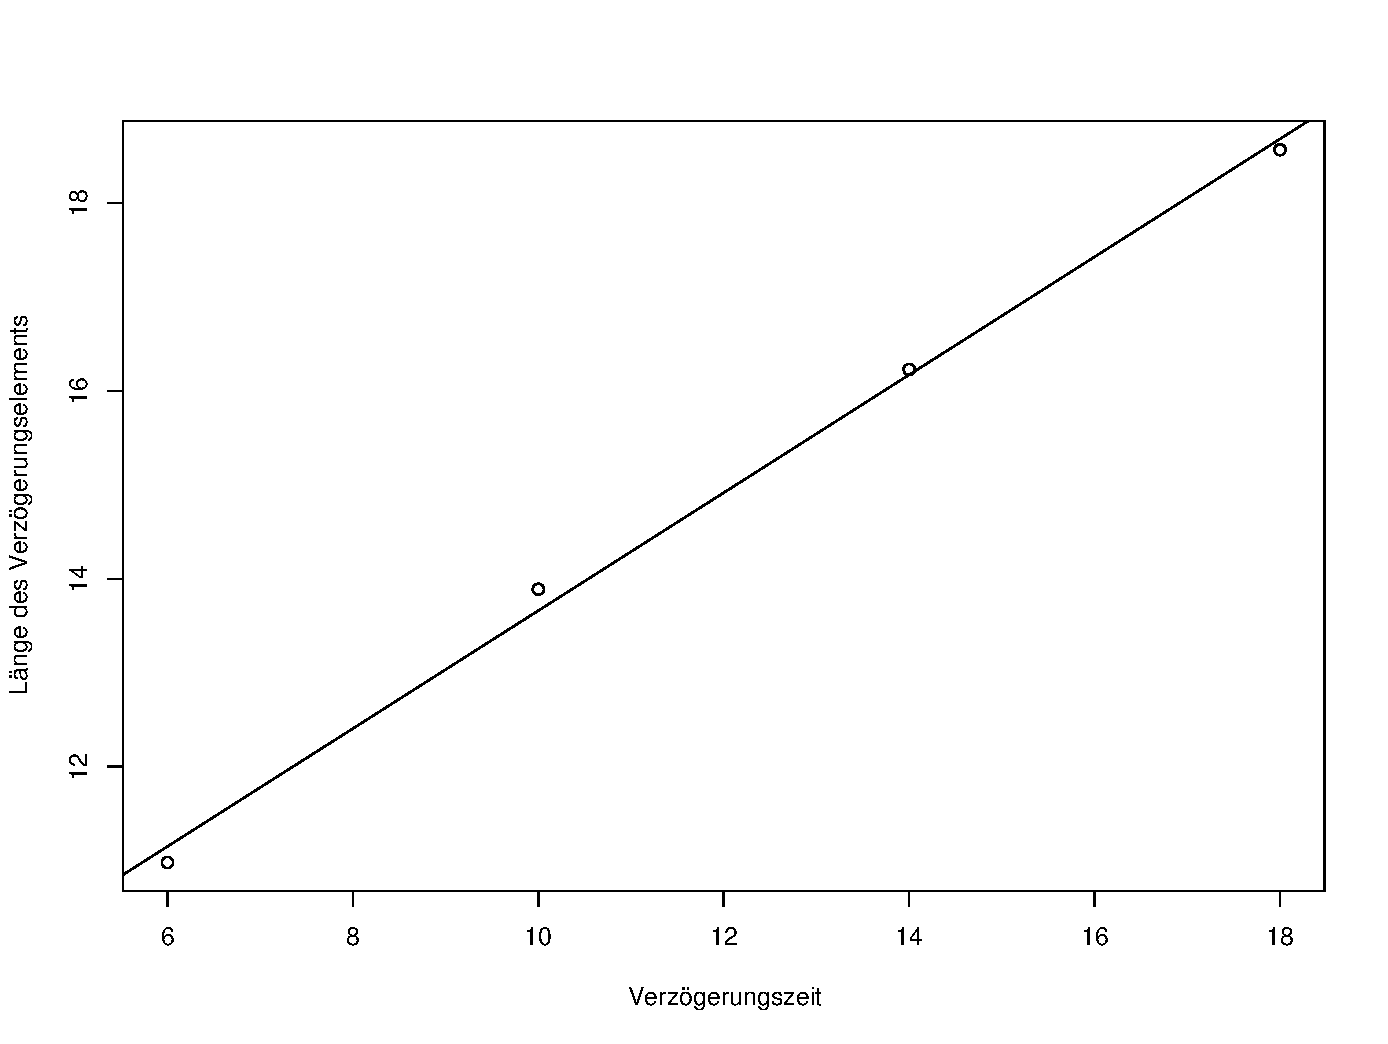
\includegraphics[width=0.7\hsize]{graphics/verzoegerungszeit}
\end{center}
\caption{Von R erzeugte graphische Darstellung der Regressionsgerade
f"ur die Verz"ogerungszeit\label{verzoegerungszeit}}
\end{figure}
Die Software R
\marginpar{\tiny\raggedright Statistik-Software R}
ist ein leistungsf"ahiges freies Softwarepaket f"ur statistische
Berechnungen. Mit folgenden Befehlen kann das obige Regressionsproblem
mit R gel"ost, und die Graphik
Graphik \ref{verzoegerungszeit} dargestellt
werden:

{\footnotesize
\begin{verbatim}
> zeit = c(6,10,14,18)
> laenge = c(10.98, 13.89, 16.23, 18.57)
> laenge.lm = lm(laenge ~ zeit)
> summary(laenge.lm)

Call:
lm(formula = laenge ~ zeit)

Residuals:
     1      2      3      4 
-0.171  0.228  0.057 -0.114 

Coefficients:
            Estimate Std. Error t value Pr(>|t|)   
(Intercept)  7.38450    0.31608   23.36  0.00183 **
zeit         0.62775    0.02468   25.43  0.00154 **
---
Signif. codes:  0 `***' 0.001 `**' 0.01 `*' 0.05 `�'0.1 ` ' 1 

Residual standard error: 0.2208 on 2 degrees of freedom
Multiple R-Squared: 0.9969,	Adjusted R-squared: 0.9954 
F-statistic: 646.9 on 1 and 2 DF,  p-value: 0.001542 

> plot(laenge ~ zeit, xlab="Verzoegerungszeit",
  ylab="Laenge des Verzoegerungselements")
> abline(laenge.lm)
\end{verbatim}}
}
R kann von \url{http://www.r-project.org} heruntergeladen werden.

%SourceDoc ws-skript.tex
%
% c04-verteilung.tex
%
% (c) 2006 Prof. Dr. Andreas M�ller
% $Id: c04-verteilung.tex,v 1.19 2008/09/09 14:22:16 afm Exp $
%
\rhead{Verteilung}
\chapter{Wahrscheinlichkeitsverteilung\label{chapter-wahrscheinlichkeitsverteilung}}
Mit dem Begriff der Ereignisalgebra kann man nur dann Wahrscheinlichkeiten
und Erwartungswerte einfach berechnen, wenn nur endlich viele 
Elementarereignisse "uberhaupt vorkommen. Schon das Beispiel der
Messungen auf der reellen Achse hat gezeigt, dass man mit diesem
Begriff zwar sch"one Ereignis-Diagramme zeichnen kann, aber die Berechnung
zum Beispiel von Wahrscheinlichkeiten schwierig wird.

\section{Wahrscheinlichkeitsverteilung}
\begin{figure}
\begin{center}
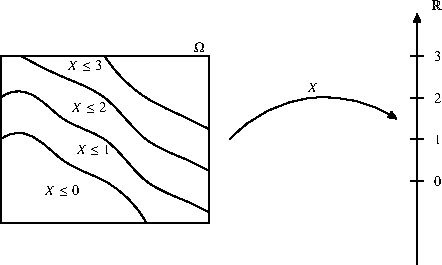
\includegraphics[width=0.9\hsize]{images/verteilungsfunktion-1}
\end{center}
\caption{"Ubergang von der Ereignisalgebra $(\Omega,{\cal A})$ zu Werten
der Zufallsvariablen $X$\label{bilduebergangzurverteilungsfunktion}}
\end{figure}
In diesem Abschnitt suchen wir daher nach einer Methode, mit der
man zuf"allige Ereignisse besser in den Griff bekommen kann, wenn
damit reelle Werte verbunden sind. Es geht also um Situationen, wo
man neben der Ereignisalgebra $(\Omega,{\cal A})$ auch noch eine
Zufallsvariable $X\colon \Omega\to\mathbb{R}$ hat. 

\subsection{Verteilungsfunktion}
\index{Verteilungsfunktion}
\begin{figure}
\begin{center}
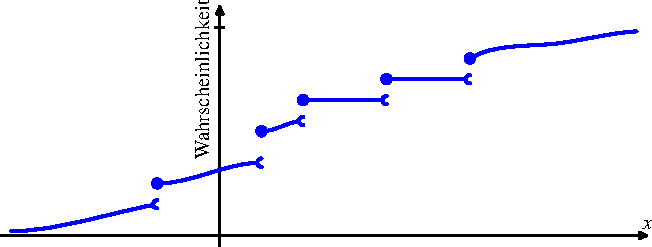
\includegraphics{images/verteilungsfunktion-2}
\end{center}
\caption{Die Verteilungsfunktion $F$ einer Zufallsvariablen $X$,
$F(x)=P(X\le x)$, zeigt die Wahrscheinlichkeit daf"ur, dass $X$ den Wert $x$ nicht "uberschreitet\label{bildverteilungsfunktion}}
\end{figure}
Aus einem Wahrscheinlichkeitsmass $P$ auf $\Omega$ kann man mit Hilfe
von $X$ auch ein Wahrscheinlichkeitsmass auf $\mathbb{R}$ bilden. F"ur die
Wahrscheinlichkeit f"ur das Intervall $[a,b]\subset\mathbb{R}$ setzt
man einfach
\[
P((a,b])=P(a< X\le b)=P(X^{-1}((a,b])),
\]
das letzte $P$ ist dabei als Wahrscheinlichkeit eines Ereignisses $\Omega$
bereits bekannt.
Noch etwas handlicher ist die folgende Definition

\begin{definition}
Die Funktion $F\colon\mathbb{R}\to\mathbb{R}:x\mapsto P(X\le x)$
heisst Verteilungsfunktion von $P$.
\end{definition}
Die Funktion ist immer eine monoton wachsende Funktion, denn
\[
F(b)-F(a)=P(a<X\le b)\ge 0\quad\text{falls}\quad a\le b.
\]
Die Wahrscheinlichkeit des sicheren Ereignisses ist 1, also
$\lim_{x\to\infty}F(x)=1.$
Die Verteilungsfunktion $F$ beinhaltet alle Information, um $P$ zu
rekonstruieren. Man kann mit ihrer Hilfe auch die Wahrscheinlichkeit
abgeschlossener Intervalle oder offener Intervalle berechnen:
\begin{satz} Sei $F$ die Verteilungsfunktion der Zufallsvariablen $X$,
dann gilt
\begin{eqnarray*}
P((a,b])&=&F(b)-F(a)\\
P([a,b])&=&\lim_{\xi\to a-} P((\xi,b])=F(b)-\lim_{\xi\to a-}F(\xi)\\
P((a,b))&=&\lim_{\xi\to b-} P((a,\xi])=\lim_{\xi\to b-}F(\xi)-F(a)\\
P([a,b))&=&\lim_{\eta\to b-}\lim_{\xi\to a-} P((\xi,\eta])=\lim_{\eta\to b-}F(\eta)-\lim_{\xi\to a-}F(\xi)\\
\end{eqnarray*}
\end{satz}
\begin{proof}[Beweis]Durch Nachrechnen unmittelbar aus den Definitionen.
\end{proof}
Als Spezialfall erh"alt man auch die Wahrscheinlichkeit f"ur einen einzelnen
Wert
\[
P(a)=P([a,a])=F(a)-\lim_{\xi\to a-}F(\xi).
\]
Solange die Funktion $F$ stetig ist, wird diese Wahrscheinlichkeit
verschwinden. Andernfalls hat die Verteilungsfunktion am Punkt $a$ eine
Sprungstelle, und die Wahrscheinlichkeit, dass der Wert $a$ eintritt,
ist gerade die Sprungh"ohe.

Man kann zeigen, dass eine monotone Funktion nur abz"ahlbar viele Sprungstellen
hat. Es gibt also eine Folge $(a_k)_{k\in\mathbb{N}}$, welche alle
Sprungstellen enth"alt. Diese Werte zeichnen sich dadurch aus, dass ihre
Wahrscheinlichkeit nicht $0$ ist und der Sprungh"ohe entspricht:
\[
P(a_k)=F(a_k)-\lim_{x\to a_k-}F(x).
\]
Aus diesen Sprungstellen kann man jetzt eine Funktion konstruieren,
die nur die Sprungstellen ber"ucksichtigt:
\[
F_d(x)=\sum_{k=1, a_k\le x}^\infty P(a_k)
\]
Die Funktion $F_d$ hat genau die gleichen Sprungstellen wie $F$, und
auch die gleichen Sprungh"ohen. $F_d$ kann sich nur "andern, wenn in der
Summe ein neuer Summand hinzukommt, also is $F_d$ zwischen den Sprungstellen
konstant.
\index{Sprungstelle}

\begin{figure}
\begin{center}
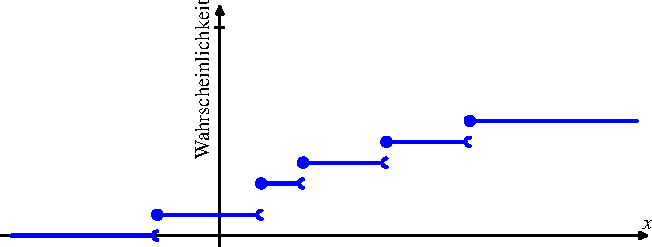
\includegraphics{images/verteilungsfunktion-3}
\[
+
\]
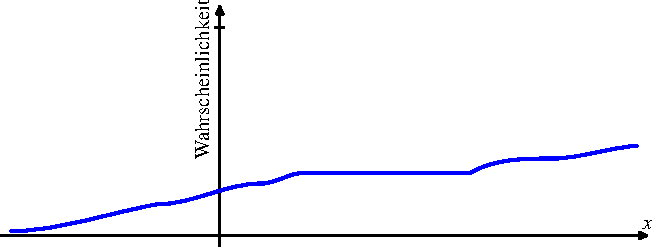
\includegraphics{images/verteilungsfunktion-4}
\[
=
\]
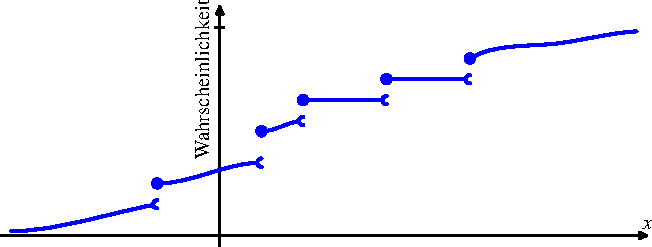
\includegraphics{images/verteilungsfunktion-2}
\end{center}
\caption{Zerlegung einer beliebigen Verteilungsfunktion (unten) in diskrete (oben)
und stetige (mitte) Komponente\label{bildzerlegungverteilungsfunktion}}
\end{figure}
\index{Verteilung!diskrete}
\index{Verteilung!stetige}

Die Differenz $F_s=F-F_d$ kann offensichtlich keine Sprungstellen haben,
wenigstens kein Sprungstellen bei Ann"aherung von links. Damit liegt
die Vermutung nahe, dass $F_s$ eine stetige Funktion ist (daher der Index
$s$). Das ist tats"achlich so:
\begin{satz}Eine Verteilungsfunktion $F$ kann immer zerlegt werden in eine
st"uckweise konstante, monoton wachsende, rechtsseitig stetige Funktion
$F_d$ und eine stetige Funktion $F_s$:
\[
F=F_d+F_s,
\]
ausserdem ist diese Zerlegung eindeutig.
\end{satz}
Die Zerlegung der Verteilungsfunktion $F$ ist in
Abbildung~\ref{bildzerlegungverteilungsfunktion} dargestellt.
\begin{proof}[Beweis]
Es gen"ugt offensichtlich zu zeigen, dass $F$ rechtsseitig stetig ist, also
keine Sprungstellen bei Ann"aherung von rechts hat. Die Differenz
$F(a+\varepsilon)-F(a)$ ist die Wahrscheinlichkeit, dass der Wert der
Zufallsvariable in das Intervall $(a,a+\varepsilon]$
f"allt. Es genugt, wenn man f"ur $\varepsilon=\frac1n$ zeigen kann,
dass $F(a+\frac1n)\to F(a)$. Das Intervall $(a,a\frac1n]$ kann man
als Vereinigung unendlich vieler kleiner Teilintervalle
schreiben, also
\[
\left(a,{\textstyle a+\frac1n}\right]
= \left(a,a+{\textstyle \frac1N}\right]\cup
\bigcup_{k=n}^{N-1}\left(a+{\textstyle\frac1{k+1}},a+{\textstyle\frac1k}\right],
\]
wobei die Teilintervalle alle disjunkt sind.
Nimmt man nun die Wahrscheinlichkeit auf beiden Seiten, folgt aus den
Axiomen f"ur $P$
\[
P\left(\left(a,a+{\textstyle\frac1n}\right]\right)
= P\left(\left(a,a+{\textstyle \frac1N}\right]\right)+
\sum_{k=n}^{N-1}P\left(\left(a+{\textstyle\frac1{k+1}},a+{\textstyle\frac1k}\right]\right)
\]
Der Ausdruck $P\left(\left(a,a+{\frac1N}\right]\right)$ ist also der
Rest einer unendlichen Reihe mit ausschliesslich positiven Gliedern,
mit der $P\left(\left(a,a+{\textstyle\frac1n}\right]\right)$
berechnet werden kann.  Nach den Axiomen f"ur $P$ gilt wegen
\[
\left(a,{\textstyle a+\frac1n}\right]
= 
\bigcup_{k=n}^{\infty}
\left(a+{\textstyle\frac1{k+1}},a+{\textstyle\frac1k}\right]
\]
auch
\[
P\left(\left(a,{\textstyle a+\frac1n}\right]\right)
= 
\sum_{k=n}^{\infty}
P\left(\left(a+{\textstyle\frac1{k+1}},a+{\textstyle\frac1k}\right]\right)
\]
d.h. die Reihe ist konvergent. Also streben die einzelnen Glieder gegen null,
oder
\[
0=\lim_{n\to\infty}P\left(\left(a,{\textstyle a+\frac1n}\right]\right)
=\lim_{n\to\infty}F(a+{\textstyle\frac1n}) - F(a)=\lim_{x\to a+} F(x)-F(a),
\]
also genau die Aussage, dass die rechtsseitigen Grenzwerte mit den
Funktionswerten "ubereinstimmen, mithin die Funktion $F$ rechtsseitig
stetig ist. Somit ist $F_s$ rechts- und linksseitig stetig.
\end{proof}
Im Allgemeinen besteht also eine Verteilungsfunktion $F$ aus einem
Teil, der Spr"unge darstellt, also bestimmte Werte der Zufallsvariable,
die mit nicht verschwindender Wahrscheinlichkeit auftreten k"onnen, und
einem Teil, der ``verschmiert'' ist "uber den ganzen Wertebereich. Wir
betrachten jeden dieser Teile separat.

\subsubsection{St"uckweise konstante Verteilungsfunktion}
\begin{figure}
\begin{center}
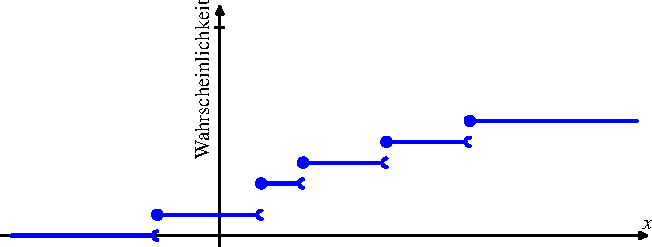
\includegraphics{images/verteilungsfunktion-3}
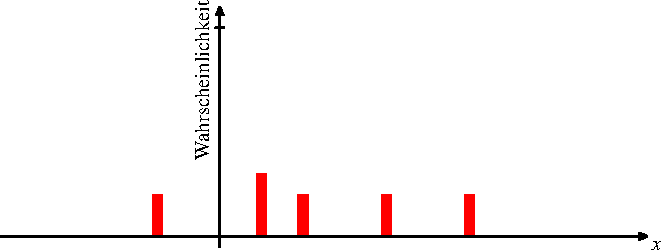
\includegraphics{images/verteilungsfunktion-5}
\end{center}
\caption{Verteilungsfunktion (oben) und Wahrscheinlichkeiten einzelner
$x$-Werte (unten) einer diskreten Verteilung
\label{bilddiskreteverteilungsfunktion}}
\end{figure}
Ist die Verteilungsfunktion st"uckweise konstant, dann ist
$P((a,b])=0$ falls im Intervall $(a,b]$ keine Sprungstelle
vorhanden ist. Ist $x_0$ eine Sprungstelle, dann ist ihr H"ohe
\[
\lim_{a\to x_0-}P((a,x_0])=\lim_{a\to x_0-}(F(x_0)-F(a))
F(x_0)-\lim_{a\to x_0-}F(a).
\]
Dies bedeutet, dass $P(\{x_0\})=F(x_0)-\lim_{a\to x_0-}F(a)$.
Offensichtlich haben also nur die Sprungwerte der Funktion eine
von 0 verschiedene Wahrscheinlichkeit, alle anderen Intervalle ohne
einen Sprungpunkt haben Wahrscheinlichkeit 0. Die Wahrscheinlichkeiten
der einzelnen Sprungwerte k"onnen wie in
Abbildung~\ref{bilddiskreteverteilungsfunktion} visualisiert werden.

Ist $S=\{x|F(x)\ne \lim_{a\to x-}F(a)\}$ die Menge der Sprungpunkte 
der Verteilungsfunktion, dann kann man damit Wahrscheinlichkeiten und
Erwartungswerte wie folgt berechnen. Die Wahrscheinlichkeit eines
Ereignisses h"angt davon ab, welches Sprungpunkte es enth"alt:
\[
P(A)=\sum_{x\in S}P(\{x\}),
\]
der Erwartungswert von $f(X)$ ist
\[
E(f(X))=\sum_{x\in S}f(x)P(\{x\}).
\]
Man kann also alle relevanten Gr"ossen berechnen, wenn man f"ur jede
Sprungstelle deren Wahrscheinlichkeit weiss, also die Funktion
\[
p\colon S\to\mathbb{R}:x\mapsto p(x)=P(\{x\}).
\]
Diese Funktion muss nat"urlich den Eigenschaften einer
Wahrscheinlichkeitsfunktion Rechnung tragen, was erf"ullt ist, wenn
$p(x)\ge 0\forall x\in S$ und 
\[
\sum_{x\in S}p(x)=1.
\]
\begin{definition}Die Funktion $p\colon S\to\mathbb{R}:x\mapsto p(x)$
heisst diskrete Wahrscheinlichkeitsverteilung auf der Menge $S$.
\end{definition}
\begin{satz}F"ur eine diskrete Wahrscheinlichkeitsverteilung $p$ gilt
\begin{enumerate}
\item $\displaystyle P(A)=\sum_{x\in A\cap S}p(x)$,
\item $\displaystyle E(f(X))=\sum_{x\in S}f(x)p(x)$
\end{enumerate}
\end{satz}

\subsubsection{Stetige Verteilungsfunktion}
\begin{figure}
\begin{center}
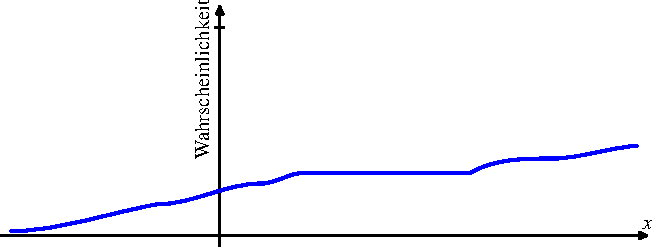
\includegraphics{images/verteilungsfunktion-4}
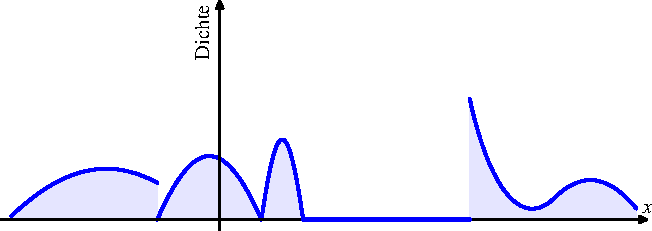
\includegraphics{images/verteilungsfunktion-6}
\end{center}
\caption{Verteilungsfunktion (oben) und Wahrscheinlichkeitsdichte 
(unten) einer stetigen Verteilung\label{bildstetigeverteilungsfunktion}}
\end{figure}
Die Formel
\[
P((a,b])=F(b)-F(a)
\]
erinnert an die Berechnung eines Integrals mit Hilfe einer
Stammfunktion.
W"are $F$ differenzierbar, k"onnte man die Ableitung bilden,
$F$ w"are dann eine Stammfunktion von $\varphi=F'$. Dann g"alte
\[
P(X\le x)=F(x)=\int_{-\infty}^x\varphi(\xi)\,d\xi.
\]
Im Allgemeinen ist selbst eine stetige Verteilungsfunktion nicht
differenzierbar.
Trotzdem gibt es dank eines Satzes, den wir hier nicht beweisen,
immer eine Funktion $\varphi$, die sich "ahnlich verh"alt wie die
Ableitung.
\begin{definition}
Die Funktion $\varphi$ heisst Wahrscheinlichkeitsdichte der Verteilungsfunktion
\index{Wahrscheinlichkeitsdichte}
\index{Dichtefunktion}
$F$ falls
\[
P(X\le x)=F(x)=\int_{-\infty}^x\varphi(\xi)\,d\xi
\]
gilt.
Man spricht in diesem Fall von einer stetigen Wahrscheinlichkeitsverteilung.
\end{definition}
Abbildung \ref{bildstetigeverteilungsfunktion} zeigt die
Wahrscheinlichkeitsdichte der stetigen Komponente der Verteilungsfunktion
aus Abbildung \ref{bildverteilungsfunktion}.

Bei diskreten Wahrscheinlichkeitsverteilungen folgte die Formel f"ur den
Erwartungswert von $X$ sofort aus der Definition, f"ur den stetigen
Fall haben wir aber noch keine exakte Definition. Wenn wir $\mathbb{R}$
in viele kleine Intervalle $I_1=(\underline x_1,\overline x_1],\dots, I_n$
unterteilen, dann gilt
\[
\sum_{i}P(I_i)\underline x_i\le
E(X)
\le
\sum_{i}P(I_i)\overline x_i
\]
Da die Wahrscheinlichkeit des Intervalls $I_i$ mit Hilfe der
Wahrscheinlichkeitsdichte berechnet werden kann:
$P(I_i)=\int_{\underline x_i}^{\overline x_i}\varphi(\xi)\,d\xi,$
kann man die Ungleichung noch etwas weiter fassen:
\[
\sum_{i}\underline x_i\bigl(\min_{\xi\in I_i}\varphi(\xi)\bigr)(\overline x_i-\underline x_i)\le
E(X)
\le
\sum_{i}\overline x_i\bigl(\max_{\xi\in I_i}\varphi(\xi)\bigr)(\overline x_i-\underline x_i)
\]
L"asst man jetzt die Intervalll"ange immer kleiner werden, wird wegen der
Stetigkeit von $\varphi$ der Unterschied zwischen
$\max_{\xi\in I_i}\varphi(\xi)$ und
$\min_{\xi\in I_i}\varphi(\xi)$ beliebig klein, und auch jener
zwischen $\underline x_i$ und $\overline x_i$. Beim Grenz"ubergang
zu beliebig kleinen Intervallen werden die beiden Seiten der Ungleichung
gegen das Integral
\[
\int_{-\infty}^{\infty}x\varphi(x)\,dx
\]
streben, d.h. der folgende Satz kann als Definition des Erwartungswertes
gesehen werden:
\begin{satz}
Ist $X$ eine Zufallsvariable mit stetiger
Wahrscheinlichkeitsverteilung mit Wahrscheinlichkeitsdichte
$\varphi$, dann
ist die Verteilungsfunktion $F$ "uberall dort differenzierbar, wo
$\varphi$ stetig ist, und es gilt dort
$F'(x)=\varphi(x)$.
Erwartungswerte von $X$ k"onnen mit Hilfe von
\begin{eqnarray*}
E(X)&=&\int_{-\infty}^{\infty}x\varphi(x)\,dx\quad\text{und}\\
E(f(X))&=&\int_{-\infty}^{\infty}f(x)\varphi(x)\,dx
\end{eqnarray*}
berechnet werden.
\end{satz}
\subsection{Wahrscheinlichkeit grosser Abweichungen}
Im vorhergehenden Kapitel haben wir mit dem Satz von Tschebyscheff ein
Hilfsmittel kennengelernt, welches erlaubt abzusch"atzen, dass eine
gross Abweichung vom Erwartungswert eintritt. Der Satz stellte einen
Zusammenhang mit der Varianz her:
\[
P(|X-\mu|>\varepsilon)\le\frac{\operatorname{var}(X)}{\varepsilon^2}.
\]
Es wurde damals schon bemerkt, dass f"ur ``weniger wilde'' Verteilung mit
besseren Absch"atzungen gerechnet werden kann. Insbesondere ist es mit
einer Dichtefunktion m"oglich, die Wahrscheinlichkeit einer grossen
Abweichung exakt zu berechnen:
\begin{satz} Ist $X$ eine Zufallsvariable, deren Verteilung die
Verteilungsfunktion $F$ hat, dann ist
\[
P(|X-\mu|>\varepsilon)=
1-F(\mu+\varepsilon)+\lim_{\xi\to (\mu-\varepsilon)-}F(\xi)
\]
Ist $\varphi$ eine Dichtefunktion, dann gilt
\[
P(|X-\mu|>\varepsilon)=1-\int_{\mu-\varepsilon}^{\mu+\varepsilon}\varphi(x)\,dx
\]
\end{satz}
\begin{proof}[Beweis]Die Formel f"ur die Dichtefunktion folgt offensichtlich
aus der Aussage "uber die Verteilungsfunktion, denn dann ist $F$ stetig
und der einseitige Grenzwert ist gerade der Funktionswert von $F$ an der
Stelle.
Es gen"ugt also letzteres
zu untersuchen.
\begin{eqnarray*}
P(|X-\mu|\le\varepsilon)
&=&1-P(\{X\ge\mu-\varepsilon\}\cap\{X\le\mu+\varepsilon\})\\
&=&1-F(\mu+\varepsilon)+\lim_{\xi\to (\mu-\varepsilon)-}F(\xi)
\end{eqnarray*}
\end{proof}
Eine Wahrscheinlichkeitsfunktion erlaubt also eine wesentlich
genauere Berechnung der Wahrscheinlichkeit einer grossen Abweichung,
nicht mehr nur eine grobe Absch"atzung.

\section{Beispiel: Gleichverteilung}
\index{Gleichverteilung}
Als Beispiel und zur Gegen"uberstellung stetiger und diskreter Zufallsvariablen
behandeln wir in diesem Abschnitt die diskrete und und die stetige
Gleichverteilung. Weitere Informationen zur Gleichverteilung sind
Im Abschnitt~\ref{section-gleichverteilung-stetig} zu finden.

\subsection{Ganzzahlige Gleichverteilung}
\index{Gleichverteilung!ganzzahlig}
Eine Zufallsvariable $X$ nehme die ganzzahligen Werte $\{a,a+1,\dots,b\}$ mit 
gleicher Wahrscheinlichkeit $\frac1{b-a+1}$ an.  Die Verteilungsfunktion
ist also
\[
F(x)=
\frac{\lfloor x \rfloor -a+1}{b-a+1}
\]
wobei $\lfloor x \rfloor$ die gr"osste ganze Zahl kleiner als $x$
bezeichnet:
\[
\lfloor x\rfloor = \max\{k\in\mathbb Z|k\le x\}.
\]
Die Wahrscheinlichkeitsverteilung ist
\[
P(X=x)=\begin{cases}
\frac1{b-a+1}&\qquad a\le x\le b,x\in\mathbb Z\\
0&\qquad\text{sonst}.
\end{cases}
\]
Damit kann jetzt auch Erwartungswert und Varianz bestimmt werden.
\begin{align*}
E(X)
&=
\sum_{k=a}^b kP(X=k)
=
\sum_{k=a}^b \frac{k}{b-a+1}
=
\frac1{b-a+1}\sum_{k=a}^bk^2
\\
&=
\frac1{b-a+1}\biggl(
\sum_{k=1}^bk-\sum_{k=1}^{a-1}k
\biggr)
=
\frac1{b-a+1}\biggl(
\frac{b(b+1)}2-\frac{a(a-1)}2
\biggr)
\\
&=
\frac12\frac{b^2+b-a^2+a}{b-a+1}=\frac{a+b}2.
\\
E(X^2)
&=
\sum_{k=a}^b k^2P(X=k)
=
\sum_{k=a}^b \frac{k^2}{b-a+1}
=
\frac1{b-a+1}\sum_{k=a}^bk^2
\\
&=
\frac1{b-a+1}\biggl(
\sum_{k=1}^bk^2-\sum_{k=1}^{a-1}k^2
\biggr)
=
\frac{ 2(a^2+ab+b^2)+b-a}{6}
\\
\operatorname{var}(X)
&=
\frac{ 2(a^2+ab+b^2)+b-a}{6}
-
\frac{a^2+2ab+b^2}{4}
\\
&=
\frac1{12}\bigl(
4a^2+4ab+4b^2+2b-2a-3a^2-6ab-3b^2
\bigr)
\\
&=
\frac1{12}\bigl(
a^2-2ab+b^2+2b-2a+1-1
\bigr)
=
\frac1{12}\bigl((b-a+1)^2 - 1\bigr)
\end{align*}
Die Varianz ist also im Wesentlichen die quadrierte Intervalll"ange
geteilt durch 12.

\subsection{Stetige Gleichverteilung}
\index{Gleichverteilung!stetig}
\index{Gleichverteilung!auf einem Intervall}
Eine Zufallsvariable $X$ nehme die Werte im Intervall $[a,b]$
mit gleicher Wahrscheinlichkeit an, d.~h.~f"ur jedes Teilintervall
$[\xi,\eta]\subset[a,b]$ gilt 
\[
P(\xi\le X\le \eta)=\frac{\xi-\eta}{b-a}.
\]
Die Wahrscheinlichkeitsdichte ist dann
\[
\varphi(x)=\begin{cases}
\frac1{b-a}&\qquad a\le x\le b\\
0&\qquad \text{sonst}
\end{cases}
\]
Erwartungswert und Varianz k"onnen damit direkt berechnet werden:
\begin{align*}
E(X)
&=
\int_{-\infty}^\infty x\varphi(x)\,dx
=
\int_a^bx\frac1{b-a}\,dx
=
\frac1{b-a}\left[\frac12x^2\right]_a^b
=
\frac12\frac{b^2-a^2}{b-a}
\\
&=
\frac{a+b}2
\\
E(X^2)
&=
\int_{-\infty}^{\infty}x^2\varphi(x)\,dx
=
\int_a^bx\frac1{b-a}\,dx
=
\frac1{b-a}\left[\frac13x^3\right]_a^b
=
\frac13\frac{b^3-a^3}{b-a}
\\
&=
\frac13(b^2+ab+a^2)
\\
\operatorname{var}(X)
&=
\frac13(b^2+ab+a^2)
-
\frac14(a^2+2ab+b^2)
\\
&=
\frac1{12}(4b^2+4ab+4a^2-3a^2-6ab-3b^2
=
\frac1{12}(a^2-2ab+b^2)
\\
&=
\frac{(b-a)^2}{12}.
\end{align*}
Auch in diesem Fall ist die Varianz die quadrierte Intervalll"ange
geteilt durch 12.

\section{L"osungsstrategie}
Probleme "uber Zufallsvariablen k"onnen also mit folgender L"osungsstrategie
angegangen werden.
\begin{enumerate}
\item
Zun"achst muss festgestellt werden, welche Verteilung die Zufallsvariablen
haben. Zu jeder sp"ater zu besprechenden Verteilung ist also auch
festzuhalten, f"ur welchen Zweck sie geeignet ist.
\item 
Die Verteilungen haben Parameter, die als n"achstes bestimmt werden
m"ussen.
Dazu k"onnen die bekannten Formeln f"ur Kennzahlen einer
Verteilung wie Erwartungswert oder Varianz.
So k"onnen zum Beispiel aus Erwartungswert $\mu$ und Varianz $\sigma^2$ 
einer auf einem Intervall gleichverteilten Zufallsvariable  die
Gleichungen
\begin{align*}
a+b&=2\mu\\
b^2-a^2&=12\sigma^2\quad\Rightarrow\quad b-a=\frac{6\sigma^2}{\mu}
\end{align*}
abgeleitet werden, welche $a$ und $b$ zu bestimmen erlauben. 
\item
Sobald die Parameter festliegen, k"onnen beliebige Wahrscheinlichkeiten
oder Erwartungswerte von $X$ oder Funktionen $f(X)$ ermittelt werden,
womit sich so ziemlich jede Frage beantworten l"asst.
\end{enumerate}
Im Folgenden geht es also vor allem darum, einen geeignet grossen
Katalog von Verteilungen bereitzustellen. Dazu dienen neben einigen
Grundverteilungen auch Rechenregeln, welche aus bereits bekannten
Verteilungen neue Verteilungen abzuleiten gestatten. Diese Rechenregeln
sind der Inhalt des n"achsten Abschnittes. Im folgenden Kapitel wird
dann eine Auswahl von praktisch n"utzlichen Verteilungen mit ihren
Eigenschaften vorgestellt.

\section{Rechenregeln}
Beim "Ubergang vom Wahrscheinlichkeitsraum $(\Omega,{\cal A},P)$ mit
der Zufallsvariable $X$ zur Verteilungsfunktion $F$ 
ging jede Information
"uber den Zufallsmechanismus verloren, der im Hintergrund f"ur das zuf"allige
Auftreten der verschiedenen Werte von $X$ verantwortlich war. Insbesondere
ist es bei zwei Zufallsvariablen $X$ und $Y$ nicht mehr m"oglich zu
rekonstruieren, ob sie unabh"angig oder wie gegebenenfalls die Abh"angigkeit
genau ausgesehen hat. Ohne Kenntnis von $\Omega$ ist es daher im allgemeinen
nicht mehr m"oglich, Erwartungswerte von beliebigen Funktionen von $X$ und $Y$
zu berechnen. Insbesondere $E(XY)$ l"asst sich nur berechnen, wenn man weiss,
dass $X$ und $Y$ unabh"angig sind.

Es zeigt sich also in einigen interessanten F"allen durchaus m"oglich, nur mit
Hilfe der Wahrscheinlichkeitsdichte f"ur unabh"angige
Zufallsvariable interessante Erwartungswerte zu berechnen.

\subsection{Variablentransformation}
\index{Variablentransformation}
Wendet man auf die Werte einer Zufallsvariablen eine Funktion an, entsteht
eine neue Zufallsvariable, die im Allgemeinen eine g"anzlich andere Verteilung
haben wird. In diesem Abschnitt soll die Verteilungsfunktion und falls
eine Dichte exitiert auch diese der neuen Zufallsvariablen bestimmt werden.

\index{Abbildung!umkehrbare}
Sei $f$ eine umkehrbare, differenzierbare Abbildung
$f\colon\mathbb{R}\to\mathbb{R}$. Dann ist $Y=f\circ X$ ebenfalls eine
Zufallsvariable. Bezeichnen wir die Verteilungsfunktionen von $X$ und $Y$
mit $F_X$ bzw.~$F_Y$, dann gilt offensichlich
\[
F_Y(y)=P(f\circ X\le y)=P(X\le f^{-1}(y))=F_X(f^{-1}(y))
\]
oder k"urzer $F_Y=F_X\circ f^{-1}$.

Wir nehmen nun an, dass die Verteilungsfunktionen ausserdem eine
Dichtefunktion haben, welche wir mit $\varphi_X$ bzw.~$\varphi_Y$
bezeichnen. Wir schreiben $y=f(x)$, und versuchen die obigen
Wahrscheinlichkeiten mit den Dichtefunktionen zu berechnen:
\[
P(a<Y\le b)
=\int_a^b\varphi_Y(y)\,dy
=\int_{f^{-1}(a)}^{f^{-1}(b)}\varphi_Y(f(x)) f'(x)\,dx
\]
Also muss $\varphi_Y(f(x))f'(x)$ die Wahrscheinlichkeitsdichte von
$F_X$ sein, also 
\begin{eqnarray*}
\varphi_Y(y)&=&\frac{\varphi_X(f^{-1}(y))}{f'(f^{-1}(y))}\\
\varphi_Y(f(x))&=&\frac{\varphi_X(x)}{f'(x)}
\end{eqnarray*}
Wir fassen diese Resultate in einem Satz zusammen

\begin{satz}
\label{satz-variablentransformation}
Ist $f\colon\mathbb{R}\to\mathbb{R}$ eine invertierbare
differenzierbare Funktion, deren Ableitung nirgends verschwindet,
und $X$ eine Zufallsvariable mit Verteilungsfunkion $F_X$. Dann ist
$f\circ X$ eine Zufallsvariable mit Verteilungsfunktion
$F_Y=F_X\circ f^{-1}$. Hat $F_X$ die Dichtefunktion $\varphi_X$, dann
hat $F_Y$ die Dichtefunktion
\[
\varphi_Y=\frac{\varphi_X}{f'}\circ f^{-1}.
\]
\end{satz}

Ohne zus"atzliche Annahmen ist es nicht m"oglich, Erwartungswert und
Varianz zu berechnen. Hingegen gibt es eine Gr"osse, die sich in jedem
Fall bestimmen l"asst:
\begin{definition}
Ist $X$ eine Zufallsvariable, dann heisst die Zahl $\operatorname{med}(X)$,
f"ur die
$F(\operatorname{med}(X))=\frac12$ ist, der Median von $X$. 
Falls mehrer Zahlen diese Bedingung erf"ullen, ist der Median als
deren Infimum definiert:
\[
\operatorname{med}(X)=\inf \{x\in\mathbb{R}\;|\;F(x)\ge{\textstyle \frac12}\}
\]
\end{definition}
F"ur den Median gilt $\operatorname{med}(Y)=f(\operatorname{med}(X))$.

\subsection{Standardisierung}
\index{Standardisierung}
Ein wichtiger Spezialfall ist der folgende:
aus einer Zufallsvariable $X$ mit Erwartungswert
$\mu$ und Varianz $\sigma^2$ l"asst sich eine neue Zufallsvariable $Y$ mit
Erwartungswert $0$ und Varianz $1$ konstruieren, indem man setzt
\[
Y=\frac{X-\mu}{\sigma}.
\]
Dies ist eine Variablentransformation mit der Funktion
$y=f(x)=\frac1\sigma(x-\mu)$ und der Umkehrfunktion $f^{-1}(y)=\sigma y+\mu$.
In diesem Fall kann man den Erwartungswert von $Y$ mit Hilfe der Rechenregeln
ausrechnen
\[
E(Y)=\frac1{\sigma}(E(X)-\mu)=0,
\]
und ebenso die Varianz
\[
\operatorname{var}(Y)=\frac1{\sigma^2}\operatorname{var}(X)=1.
\]
Der Satz \ref{satz-variablentransformation} l"asst sich hier unmittelbar
anwenden, es ergeben sich Verteilungs- und Dichtefunktion von $Y$
wie folgt:
\begin{eqnarray*}
F_Y(y)&=&F_X(y\sigma+\mu)\\
\varphi_Y(y)&=&\sigma\varphi_X(y\sigma+\mu)
\end{eqnarray*}
Wir fassen diese Resultate in einem Satz zusammen:

\begin{satz}
\label{satz-standardisierung}
Ist $X$ eine Zufallsvariable mit Erwartungswert $\mu$ und
Varianz $\sigma^2$, dann ist
\[
Y=\frac{X-\mu}\sigma
\]
eine Zufallsvariable mit Erwartungswert 0 und Varianz 1.
Zwischen den Verteilungsfunktionen $F_X$ bzw.~$F_Y$ von $X$ bzw.~$Y$ 
bestehen die Beziehungen
\[
F_Y(y)=F_X(y\sigma+\mu)\qquad F_X(x)=F_Y\left(\frac{x-\mu}\sigma\right)
\]
Hat die Verteilungsfunktion eine Dichte, dann gilt ausserdem
\[
\varphi_Y(y)=\sigma\varphi_X(y\sigma+\mu)\qquad
\varphi_X(x)=\frac1{\sigma}\varphi_Y\left(\frac{x-\mu}\sigma\right)
\]
\end{satz}


\subsection{Zwei Zufallsvariable}
Wir beschr"anken uns darauf, die Wahrscheinlichkeitsdichten von Summen
und Produkten von Zufallsvariablen zu berechnen, die wir als unabh"angig
voraussetzen.
Wir betrachten also zwei Zufallsvariable $X_1$ und $X_2$ mit reellen
Werten.
Da die Werte voneinander unabh"angig sind, ist
die passende Ereignisalgebra die Produktalgebra, also
$(x_1,x_2)\in
\mathbb{R}\times\mathbb{R}$,
und die Ereignisse sind kartesiches Produkte von Intervallen. Dann sind
die Wahrscheinlichkeiten $P(X_1\le x_1)$  und $P(X_2\le x_2)$ unabh"angig
voneinander, insbesondere ist $P(X_1\le x_1)=F_1(x_1)$ und
$P(X_2\le x_2)=F_2(x_2)$.

Die Wahrscheinlichkeit, dass $X_1$ in einem Intervall $(a_1,b_1]$,
$X_2$ im Intervall $(a_2,b_2]$ liegt ist 
\begin{eqnarray*}
P(a_1<X_1\le b_1\wedge a_2<X_2\le b_2)
&=& P(a_1<X_1\le b_1) P(a_2<X_2\le b_2)\\
&=&\int_{a_1}^{b_1}\varphi_1(x_1)\,dx_1
\int_{a_2}^{b_2}\varphi_2(x_2)\,dx_2\\
&=&\int_{a_1}^{b_1}dx_1
\int_{a_2}^{b_2}dx_2\,
\varphi_1(x_1) \varphi_2(x_2).
\end{eqnarray*}
Die zweidmensionale
Verteilungsfunktion $F(x_1,x_2)=P(X_1\le x_1\wedge X_2\le x_2)$ hat
also eine zweidimensionale Wahrscheinlichkeitsdichte
\[
\varphi(x_1,x_2)=\varphi_1(x_1)\varphi_2(x_2).
\]

\subsection{Summe zweier Zufallsvariable}
\index{Summe zweier Zufallsvariablen}
Seien $X_1$ und $X_2$ zwei Zufallsvariable mit Verteilungsfunktion $F_1$ und
$F_2$. Gesucht ist die Verteilungsfunktion $F$ von $X_1+X_2$, sowie die
Wahrscheinlichkeitsverteilung und gegebenenfalls die Wahrscheinlichkeitsdichte.

Zun"achst ist nach Definition der Verteilungsfunktion
\[
F(z)=P(X_1+X_2\le z).
\]
Die Berechnung von $F$ aus $F_1$ und $F_2$ verl"auft f"ur diskrete und
kontinuierliche Wahrscheinlichkeitsverteilungen verschieden.
\subsubsection{Diskreter Fall}
In diesem Fall hat $X_i$ die Wahrscheinlichkeitsverteilung
$p_i(x)$ auf der Menge $S_i$, und es gilt
\begin{eqnarray*}
F(z)&=&\sum_{x_1\in S_1, x_2\in S_2, x_1+x_2\le z}p(x_1)p(x_2)\\
&=&\sum_{x_1\in S_1}p(x_1)\sum_{x_2\in S_2, x_2 \le z - x_1}p(x_2)\\
&=&\sum_{x_1\in S_1}p(x_1) F_2(z-x_1)
\end{eqnarray*}
Oder, wenn vor allem die Wahrscheinlichkeitsverteilung interessiert:
\[
p(z)=\sum_{x_1\in S_1, x_2\in S_2, x_1+x_1=z}p(x_1)p(x_2).
\]
\subsubsection{Stetiger Fall}
Im stetigen Fall kann man schreiben
\begin{eqnarray*}
F(z)&=&\int_{-\infty}^{\infty}\int_{-\infty}^{z-x_1}\varphi_1(x_1)\varphi_2(x_2)
\,dx_2\,dx_1\\
&=&\int_{-\infty}^{\infty}
\varphi_1(x_1)
\int_{-\infty}^{z-x_1}
\varphi_2(x_2)
\,dx_2\,dx_1\\
&=&\int_{-\infty}^{\infty}
\varphi_1(x_1)
F_2(z-x_1)
\,dx_1\\
\end{eqnarray*}
Nun interesssiert uns vor allem die Wahrscheinlichkeitsdichte, also die
``Ableitung'' von $F$:
\[
\varphi(z)=\int_{-\infty}^{\infty}\varphi_1(x_1)\varphi_2(z-x_1)\,dx_1
\]
Diese Integral heisst die Faltung der Funktionen $\varphi_1$ und $\varphi_2$,
$\varphi=\varphi_1*\varphi_2$.
\index{Faltung}

\subsection{Verteilung von $X^2$}
Wir bestimmen die Wahrscheinlichkeitsdichte f"ur das Quadrat 
$X^2$ einer stetig verteilte Zufallsvariable $X$.
Sei $F_{X^2}$ die Verteilungsfunktion von $X^2$, $F_X$ jene von $X$.
Dann gilt f"ur $z\ge 0$
\begin{eqnarray*}
F_{X^2}(z)&=&P(X^2\le z)=P(-\sqrt{z}\le X\le \sqrt{z})\\
&=&F_X(\sqrt{z})-F(-\sqrt{z})\\
&=&\int_{-\infty}^{\sqrt{z}}\varphi(x)\,dx-\int_{-\infty}^{-\sqrt{z}}\varphi(x)\,dx\\
&=&\int_{-\sqrt{z}}^{\sqrt{z}}\varphi(x)\,dx
\end{eqnarray*}
F"ur negative $z$ verschwindet die Verteilungsfunktion nat"urlich, denn
die Wahrscheinlichkeit dass $X^2\le z <0$ ist nat"urlich 0.

Wir interessieren uns aber wieder nur f"ur Dichtefunktion, die wir
durch Ableiten finden k"onnen:
\[
\varphi_{X^2}(z)=\begin{cases}
\frac{1}{2\sqrt{z}}\left(\varphi_X(\sqrt{z})+\varphi_X(-\sqrt{z})\right)&\qquad z\ge 0\\
0&\qquad z<0
\end{cases}
\]
Weitere Beispiele f"ur aus mehreren unabh"angigen Zufallsvariablen
verkn"upften Verteilungen werden wir weiter unten behandeln, wobei
dann auch eine konkrete Wahrscheinlichkeitsdichtefunktion gegeben sein
wird.

\subsection{Verteilung von $\sqrt{X}$\label{verteilungsfunktion-wurzel}}
Sei $X$ eine Zufallsvariable mit $X\ge 0$. Hat $X$ Verteilungsfunktion $F_X$
und Dichtefunktion
$\varphi_X$, dann ist die Verteilungsfunktion von $\sqrt{X}$
\[
F_{\sqrt{X}}(x)=P(\sqrt{X}\le x)=P(X\le x^2)=F_X(x^2)
\]
F"ur die Dichtefunktionen bedeutet das
\[
F_{\sqrt{X}}(x)=\int_0^{x^2}\varphi_X(t)\,dt
\]
woraus man die Dichtefunktion $\varphi_{\sqrt{X}}$ durch ableiten
bestimmen kann:
\[
\varphi_{\sqrt{X}}(x)=2x\varphi_X(x^2).
\]

\subsection{Verteilung von $X/Y$\label{verteilungsfunktion-quotient}}
Seien $X$ und $Y$ Zufallsvariablen mit $Y>0$, dann ist $T=X/Y$ ebenfalls
eine Zufallsvariable. Ist $\varphi_Y$ die Dichtefunktion von $Y$,
und $F_X$ die Verteilungsfunktion von $X$, dann kann man die
Verteilungsfunktion von $T$ wie folgt berechnen:
\[
P(T\le t)=P(X\le tY)=\int_0^\infty F_X(ty)\varphi_Y(y)\,dy
\]
Die Ableitung nach $t$ ergibt die zugeh"orige Dichtefunktion
\[
\varphi_T(t)=\int_0^\infty\varphi_X(ty)y\varphi_Y(y)\,dy.
\]

\subsection{Verteilung von $XY$\label{verteilungsfunktion-produkt}}
\index{Produkt zweier Zufallsvariable}
Seien $X$ und $Y$ unabh"angige, positive Zufallsvariable, dann ist $T=XY$
ebenfalls eine Zufallsvariable. Wir suchen die Warhscheinlichkeitsdichte
$\varphi_T$ von $T$.  Zun"achst gilt nach Definition
\[
F_T(t)=P(XY\le t).
\]
Die Wahrscheinlichkeit, dass $X$ einen Wert in einem sehr schmalen Intervall
$[x,x+dx]$ annimmt ist $\varphi_X(x)\,dx$.
Damit beim Eintreffen dieses Ereignisses auch das Produkt
$XY\le t$ ist, muss $Y$ einen Wert im Intervall $[0,t/x]$ annehmen.
Also gilt wegen der Unabh"angigkeit von $X$ und $Y$
\begin{eqnarray*}
P(XY\le t\;\wedge\; X\in[x,x+dx])&=&P(X\in[x,x+dx]\;\wedge\; Y\le t/x)\\
&=&P(X\in[x,x+dx])\cdot P(Y\le t/x)\\
&=&\varphi_X(x)\,dx\cdot F_Y(t/x).
\end{eqnarray*}
Um nun die gesamte Wahrscheinlichkeit $P(XY\le t)$ zu finden, m"ussen die eben
berechneten Terme ``summiert'' werden:
\[
P(XY\le t)=\int_0^\infty\varphi_X(x)F_Y(t/x)\,dx
\]
Durch Ableiten nach $t$ findet man
\[
\varphi_{XY}(t)=\frac{d}{dt}F_{XY}(t)=\int_0^\infty \varphi_X(x)\varphi_Y(t/x)\,\frac{dx}x.
\]




%SourceDoc ws-skript.tex
%
% c04-verteilung.tex
%
% (c) 2006 Prof. Dr. Andreas M�ller
% $Id: c04a-verteilung.tex,v 1.17 2008/09/09 14:22:16 afm Exp $
%
\rhead{Verteilungen}
\chapter{Ein Katalog von Wahrscheinlichkeitsverteilungen
\label{chapter-wahrscheinlichkeitsverteilung-katalog}}
Im Laufe der Zeit ist eine grosse Zahl von Verteilungen gefunden worden,
die die verschiedensten von Zufalls beeinflussten Prozesse in der realen
Welt beschreiben. In diesem Kapitel werden einge praktisch wichtige
Verteilungen vorgestellt.
\section{Stetige Wahrscheinlichkeitsverteilungen}

\subsection{Gleichverteilung\label{section-gleichverteilung-stetig}}
\begin{figure}
\begin{center}
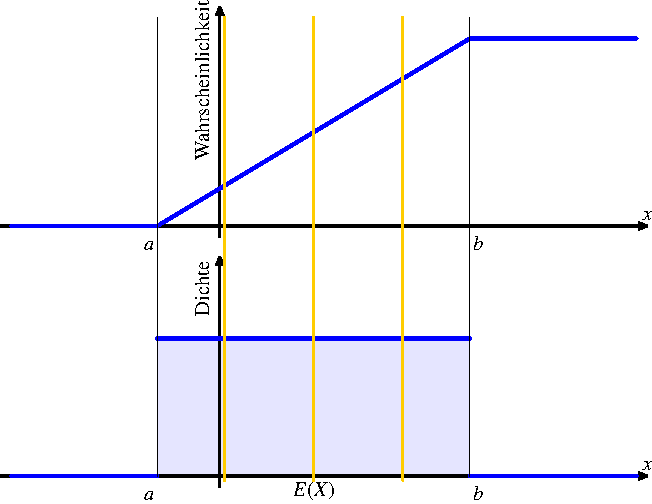
\includegraphics[width=0.8\hsize]{images/verteilungsfunktion-7}
\end{center}
\caption{Verteilungsfunktion (oben) und Wahrscheinlichkeitsdichte (unten)
der Gleichverteilung\label{bild-gleichverteilung}}
\end{figure}
\begin{figure}
\begin{center}
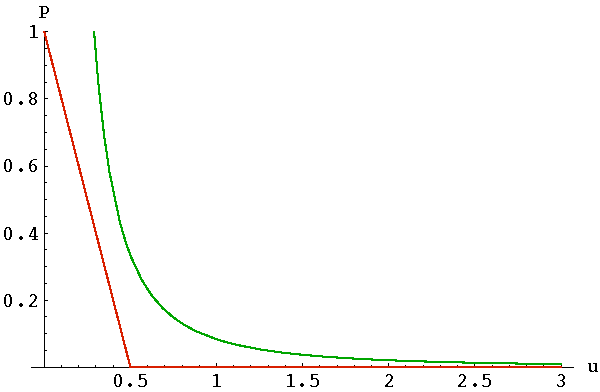
\includegraphics[width=0.8\hsize]{graphics/abwgl}
\end{center}
\caption{Wahrscheinlichkeit einer Abweichung vom Mittelwert einer
in $[0,1]$ gleichverteilten Zufallsvariable (rot) im Vergleich mit
der oberen Schranke aus dem Satz von Tschebyscheff (gr"un)
\label{bild-gleichverteilung}}
\end{figure}
Gleichverteilung der Werte einer Zufallsvariablen liegt vor, wenn
die Wahrscheinlichkeit, dass ein Wert in ein bestimmtes Interval
f"allt, der L"ange des Intervalles proportional ist. Dies bedeutet,
dass die Verteilungsfunktion $F$ konstante Steigung hat. Da $0\le F(x)\le 1$
gelten muss, ist dies nur innerhalb eines Intervals $[a,b]$ m"oglich.
\begin{definition}Die Zufallsvariable $X$ heisst auf dem Interval
$[a,b]$ gleichverteilt, wenn sie die Verteilungsfunktion
\[
F(x)=\begin{cases}
0&\qquad x< a\\
\frac{x-a}{b-a}&\qquad x\in[a,b]\\
1&\qquad x> b
\end{cases}
\]
mit der Wahrscheinlichkeitsdichte
\[
\varphi(x)=\begin{cases}
0&\qquad x< a\\
\frac1{b-a}&\qquad x\in[a,b]\\
0&\qquad x> b
\end{cases}
\]
hat.
\end{definition}

\subsubsection{Erwartungswert und Varianz}
\begin{satz}Sei $X$ eine in $[a,b]$ gleichverteilte Zufallsvariable,
dann gilt
\begin{align*}
E(X)&=\frac{a+b}2\\
\operatorname{var}(X)&=\frac{(b-a)^2}{12}
\end{align*}
\end{satz}
\begin{proof}[Beweis]
Mit Hilfe der Dichtefunktion berechnet man den Erwartungswert
\begin{align*}
E(X)&=\int_{-\infty}^\infty \varphi(x)x\,dx=\int_a^b\frac{x}{b-a}\,dx\\
&=\frac1{b-a}\left[\frac12x^2\right]_a^b=\frac{b^2-a^2}{2(b-a)}=\frac{a+b}2
\end{align*}
und die Varianz
\begin{align*}
E(X^2)=&\int_{-\infty}^\infty x^2\varphi(x)\,dx=\frac1{b-a}\int_a^bx^2\,dx\\
&=\frac1{b-a}\left[\frac{x^3}3\right]_a^b=\frac{b^3-a^3}{3(b-a)}=\frac{a^2+ab+b^2}3\\
\operatorname{var}(X)&=\frac{a^2+ab+b^2}3-\frac{(b+a)^2}4\\
&=\frac{4a^2+4ab+4b^2-3b^2-6ab-3a^2}{12}\\
&=\frac{a^2-2ab+b^2}{12}=\frac13\left(\frac{b-a}2\right)^2\\
\sqrt{\operatorname{var}(X)}&=\frac1{\sqrt{3}}\cdot\frac{b-a}2\simeq 0.57\cdot\frac{b-a}2.
\end{align*}

\end{proof}

\subsubsection{*Wahrscheinlichkeit einer grossen Abweichung}
{\small
F"ur $\varepsilon>\frac{b-a}2$ ist die Wahrscheinlichkeit
$P(|X-\mu|>\varepsilon)$
einer Abweichung vom Erwartungswert $\mu=E(X)$ nat"urlich $0$,
aber f"ur kleinere $\varepsilon$ ergibt sich
\begin{eqnarray*}
P(|X-\mu|>\varepsilon)
&=&1-\int_{\mu-\varepsilon}^{\mu+\varepsilon}\varphi(x)\,dx
=1-\int_{\mu-\varepsilon}^{\mu+\varepsilon}\frac{1}{b-a}\,dx\\
&=&1-\frac1{b-a}\left[x\right]_{\mu-\varepsilon}^{\mu+\varepsilon}=1-\frac{2\varepsilon}{b-a}
\end{eqnarray*}
}

\subsection{Exponentialverteilung\label{section-exponentialverteilung}}
\begin{figure}
\begin{center}
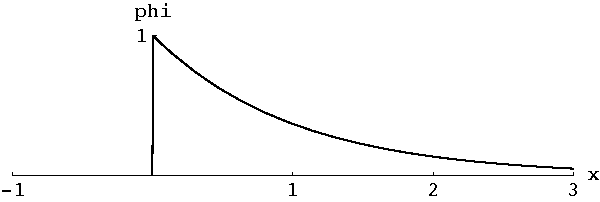
\includegraphics[width=0.8\hsize]{graphics/expphi}
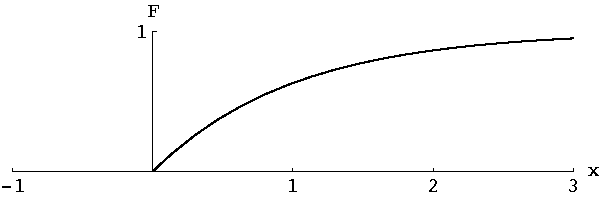
\includegraphics[width=0.8\hsize]{graphics/expF}
\end{center}
\caption{Dichtefunktion (oben) und Verteilungsfunktion (unten) der Exponentialverteilung
\label{bildexponentialverteilung}}
\end{figure}
Bei radioaktiven Stoffen und bei gewissen Bauteilen stellt man fest,
dass ihr Zerfall bzw.~ihr Versagen kein Ged"achtnis hat.
Die Wahrscheinlichkeit, dass ein Atomkern innerhalb der Zeit $t$ zerf"allt,
ist gleich gross wie die Wahrscheinlichkeit, dass er zwischen $t_0$
und $t_0+t$ zerf"allt, wenn er bis zur Zeit $t_0$ nicht zerfallen ist.
Auch Bauteile ohne Erm"udungserscheinungen verhalten sich so.

\subsubsection{Verteilungsfunktion und Dichtefunktion}
Etwas formaler sei $X$ eine Zufallsvariable, die die Zeit angibt, zu der
ein Atomkern zerf"allt. Die ``Ged"achtnislosigkeit'' bedeutet, dass die
bedingte Wahrscheinlichkeit f"ur einen Zerfall vor $t_0+t$ unter der
Annahme, dass der Kern bis zur Zeit $t_0$ nicht zerfallen ist, gleich
gross ist wie die Wahrscheinlichkeit eines Zerfalls bis zur Zeit $t$:
\[
P(X \le t) = P(X\le t_0+t|X > t_0)
\]
Dies ist nat"urlich gleichbedeutend mit der Wahrscheinlichkeit f"ur
die negierten Ereignisse:
\[
P(X > t) = P(X > t_0+t|X > t_0)
\]
Aus der Definition der bedingten Wahrscheinlichkeit
\ref{def-bedingte-wahrscheinlichkeit} folgt
\[
P(X> t_0+t|X>t_0)=\frac{P(X>t_0+t\wedge X>t_0)}{P(X > t_0)}
=\frac{P(X>t_0+t)}{P(X>t_0)}
\]
Die Bedingung an die Verteilung wird damit zu
\[
P(X>t)P(X>t_0)=P(X>t+t_0).
\]
Schreiben wir jetzt $g(t)=P(X>t)=1-F(t)$, werden die Formeln
etwas "ubersichtlicher:
\[
g(t)g(t_0)=g(t+t_0).
\]
Zun"achst leiten wir nach $t_0$ ab, wir nehmen ja an, dass wir
eine stetige Zufallsvariable haben, und dass die Verteilungsfunktion
differenzierbar sein wird.
Wir erhalten
\[
g(t)g'(t_0)=g'(t+t_0).
\]
Jetzt lassen wir $t_0$ gegen $0$ streben, und bekommen
die Differentialgleichung
\[
g'(t)=g'(0)g(t)
\]
f"ur $g(t)$.
Diese lineare Differentialgleichung erster Ordnung
muss als L"osung eine Exponentialfunktion haben. Da $F(t)$
monoton w"achst, muss $g(t)$ monoton fallen, ausserdem
muss $g(t)$ beschr"ankt bleiben. Damit bleibt nur
$g(t)=e^{-at}$ mit einem positiven $a$.

\begin{definition}
Die Wahrscheinlichkeitsverteilung mit Dichtefunktion
\[
\varphi(x)=\begin{cases}
0&\qquad x<0\\
a e^{-a x}&\qquad x\ge 0
\end{cases}
\]
heisst Exponentialverteilung. Ihre Verteilungsfunktion ist
\[
F(x)=\begin{cases}
0&\qquad\text{f"ur $x < 0$}\\
1-e^{-ax}&\qquad\text{f"ur $x\ge 0$}.
\end{cases}
\]
\end{definition}
\index{Exponentialverteilung}
\index{Verteilungsfunktion!Exponentialverteilung}
\index{Wahrscheinlichkeitsdichte!Exponentialverteilung}
Wir sollten noch nachrechnen, dass dies tats"achlich die richtige
Verteilungsfunktion ist. Zun"achst w"achst sie tats"achlich monoton,
und auch der Grenzwert f"ur $t\to\infty$ ist wie gew"unscht. Aber
auch die Ableitung ist richtig:
\[
\frac{d}{dt}(1-e^{-at})=ae^{-at}\qquad\text{f"ur}\quad t>0.
\]

\subsubsection{Erwartungswert und Varianz}
\index{Erwartungswert!der Exponentialverteilung}
\index{Exponentialverteilung!Erwartungswert}
\index{Varianz!der Exponentialverteilung}
\index{Exponentialverteilung!Varianz}
\begin{satz}Eine exponentialverteilte Zufallsvariable $X$ mit Parameter
$a$ hat folgenden Erwartungswert und folgene Varianz:
\begin{eqnarray*}
E(X)&=&\frac1a\\
\operatorname{var}(X)&=&\frac1{a^2}
\end{eqnarray*}
\end{satz}
\begin{proof}[Beweis]
Zur Berechnung von Erwartungswert und Varianz ist es n"utzlich die Integrale
$I_n=\int \xi^ne^{-\xi}\,d\xi$
berechnen zu k"onnen. Diese findet man rekursiv durch partielle Integration:
\begin{eqnarray*}
I_n&=&\int \xi^ne^{-\xi}\,d\xi\\
&=&-\xi^ne^{-\xi}+n\int \xi^{n-1}e^{-\xi}\,d\xi\\
&=&-\xi^ne^{-\xi}+nI_{n-1}
\end{eqnarray*}
Um Erwartungswert und Varianz zu berechnen, verwendet man mit Vorteil die
Variablentransformation $ax=\xi$. F"ur den Erwartungswert ergibt sich:
\begin{align*}
E(X)&=\int_0^{\infty}ae^{-ax}x\,dx
=\frac1a\int_0^{\infty}ax e^{-ax}a\,dx
=\frac1a\int_0^{\infty}\xi e^{-\xi}\,d\xi\\
&=\frac1a\left[-\xi e^{-\xi}-e^{-\xi}\right]_0^\infty=\frac1a
\end{align*}
Analog f"ur die Varianz:
\begin{align*}
E(X^2)
&=
\int_0^{\infty}x^2ae^{-ax}\,dx
=\frac1{a^2}\int_0^{\infty}(ax)^2e^{-ax}a\,dx\\
&=\frac1{a^2}\int_0^{\infty}\xi^2e^{-\xi}\,d\xi
=\frac1{a^2}\left[\xi^2e^{-\xi}-2\xi e^{-\xi}+2e^{-\xi}\right]_0^\infty
=\frac2{a^2}
\\
\operatorname{var}(X)
&=E(X^2)-E(X)^2=\frac2{a^2}-\left(\frac1a\right)^2=\frac1{a^2}
\end{align*}
\end{proof}
Die Gr"osse $\frac1a$ l"asst sich also leicht interpretiren: sie ist die
mittlere ``Lebensdauer'', man findet sie oft unter dem K"urzel MTBF f"ur
mean time between failure.
Und $\sqrt{\operatorname{var}(X)}$ 
ist genau gleich gross. 
\index{Mean time between failure}
\index{MTBF}
\subsubsection{*Wahrscheinlichkeit grosser Abweichungen}
{
\small
\begin{figure}
\begin{center}
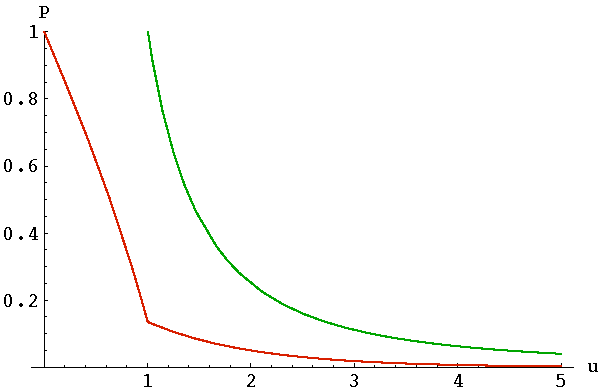
\includegraphics[width=0.8\hsize]{graphics/abwexp}
\end{center}
\caption{Wahrscheinlichkeit f"ur eine grosse Abweichung bei einer
Exponentialverteilten Zufallsvariable, oben die durch den Satz von Tschebyscheff egebene Schranke (gr"un), unten die exakte Rechnung mit
Hilfe der Exponentialvereteilung (rot)\label{abweichung-exponential}}
\end{figure}
Wir k"onnen nun auch die Wahrscheinlichkeit einer grossen Abweichung
berechnen:
\begin{satz} F"ur eine exponentialverteilte Zufallsvariable mit
Erwartungswert $\frac1a$ ist die Wahscheinlichkeit einer Abweichung
$\varepsilon$ vom Erwartungswert
\[
P(|X-{\textstyle\frac1a}|>\varepsilon)=
\begin{cases}
e^{-a\varepsilon-1}&\qquad\text{f"ur $\varepsilon > \frac1a$}\\
1-e^{a\varepsilon-1}+e^{-a\varepsilon-1}&\qquad\text{f"ur $\varepsilon \le \frac1a$}
\end{cases}
\]
\end{satz}
\begin{proof}[Beweis]
Die Wahrscheinlichkeit einer grossen Abweichung ist
\begin{eqnarray*}
P(|X-{\textstyle\frac1a}|>\varepsilon)
&=&1-\int_{\frac1a-\varepsilon}^{\frac1a+\varepsilon}\varphi_a(x)\,dx\\
&=&1-\int_{\max(0,\frac1a-\varepsilon)}^{\frac1a+\varepsilon}ae^{-ax}\,dx\\
&=&1-\left[-e^{-ax}\right]_{\max(0,\frac1a-\varepsilon)}^{\frac1a+\varepsilon}\\
&=&1+e^{-a\varepsilon-1}-e^{-\max(0,1-a\varepsilon)}\\
&=&\begin{cases}
e^{-a\varepsilon-1}&\qquad\text{f"ur $\varepsilon > \frac1a$}\\
1-e^{a\varepsilon-1}+e^{-a\varepsilon-1}&\qquad\text{f"ur $\varepsilon \le \frac1a$}
\end{cases}
\end{eqnarray*}
\end{proof}
Der Satz von Tschebyscheff setzt diese Wahrscheinlichkeit in Relation
zur Varianz
\[
P(|X-{\textstyle\frac1a}|>\varepsilon)\le
\frac{\operatorname{var}(X)}{\varepsilon^2}=\frac{1}{a^2\varepsilon^2},
\]
selbstverst"andlich muss diese Ungleichung immer noch erf"ullt sein.
Also
\begin{alignat*}{3}
e^{-a\varepsilon-1}&\le&\frac1{a^2\varepsilon^2}&\qquad\text{f"ur $a\varepsilon>1$}\\
1-e^{a\varepsilon-1}+e^{-a\varepsilon-1}&\le&\frac1{a^2\varepsilon^2}&\qquad\text{f"ur $a\varepsilon\le1$}
\end{alignat*}
In allen Ausdr"ucken kommt immer nur das Produkt $a\varepsilon$ vor,
wir k"onnen daher
abk"urzend $u=a\varepsilon$ schreiben. Die zweite Ungleichung wird dann zu
\[
\frac{1-e^{u}+e^{-u}}e\le\frac1{u^2}\qquad\text{f"ur $u\le1$}
\]
In diesem Fall ist die rechte Seite mindestens 1,
die Tschebyscheff-Ungleichung wird jetzt v"ollig nichtssagend, denn 
gr"osser als 1 kann die Wahrscheinlichkeit f"ur eine Abweichung ohnehin
nicht werden.

Die erste Ungleichung wird zu
\[
e^{-u-1}\le\frac1{u^2}\qquad\text{f"ur $u > 1$}.
\]
Diese Funktion f"allt monoton sehr schnell gegen 0, viel schneller
als der Ausdruck $\frac1{u^2}$. In der Abbildung~\ref{abweichung-exponential}
sieht man beide Schranken, die allgemeine, gegeben durch den
Satz von Tschebyscheff, und die exakte f"ur die Exponentialverteilung.
}

\subsubsection{Anwendung}
Ger"ate aller Art versuchen, die Lebensdauer dadurch zu erh"ohen, dass
kritische Komponenten redundant aufgebaut werden.
Zum Beispiel verwenden Server h"aufig zwei Disks, deren Daten
gespiegelt sind, so dass der Ausfall eines Disks noch keinen Ausfall
des Gesamtsystems verursacht. Wir wollen die erwartete Zeit bis zum
Ausfall des Gesamtsystems berechnen, wenn zwei Disks verwendet werden,
deren Zeit bis zum Ausfall exponentialverteilt ist. Weiter nehmen
wir an, dass die Disks unabh"angig voneinander ausfallen.

Sei also $X_i$ die Zeit bis zum Ausfall von Disk $i$, mit
Verteilungsfunktion $F_{X_i}(t)=1-e^{at}$ f"ur $t\ge 0$. Gesucht
ist die Verteilungsfunktion f"ur die Zeit $X$ bis zum Ausfall
des Gesamtsystems, also die Funktion $F(t)=P(X\le t)$. Das Gesamtsystem
f"allt aus, wenn beide Disks ausgefallen sind, es ist also
\begin{align*}
F(t)
&=P(X\le t)=P(X_1\le t\wedge X_2\le t)\\
&=P(X_1\le t)\cdot P(X_2\le t)
= F_{X_1}(t) F_{X_2}(t)=(1-e^{-at})^2
\end{align*}
Zur Berechnung des Erwartungswertes von $X$ wird die
Wahrscheinlichkeitsdichte ben"otigt, also die Ableitung davon:
\[
\varphi_{X}(t)=2(1-e^{-at})ae^{-at}.
\]
Damit wird der Erwartungswert
\begin{align*}
E(X)
&=
\int_{-\infty}^{\infty}t\varphi_X(t)\,dt
=\int_0^\infty 2x(1-e^{-at})ae^{-at}\,dt
\\
&=2\int_0^\infty axe^{-at}\,dt - \int_0^\infty t (2a)e^{-(2a)t}\,dt
=2\cdot\frac1a-\frac1{2a}=\frac{4-1}2\cdot\frac1a=\frac23\cdot\frac1a.
\end{align*}
Durch Redundanz l"asst sich die mittlere Zeit bis zu einem Ausfall
also nur um 50\% steigern, die Kosten f"ur das Disksystem werden
aber mehr als verdoppelt.


\subsection{Normalverteilung\label{normalverteilung}}
\index{Normalverteilung}
\begin{figure}
\begin{center}
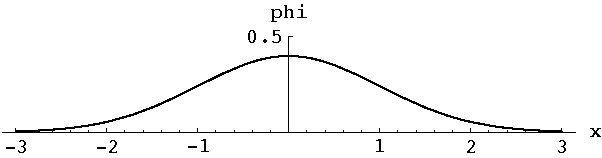
\includegraphics[width=0.8\hsize]{graphics/normphi}
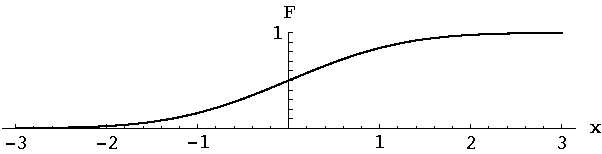
\includegraphics[width=0.8\hsize]{graphics/normF}
\end{center}
\caption{Dichtefunktion (oben) und Verteilungsfunktion (unten) der Normalverteilung\label{bildnormalverteilung}}
\end{figure}
Die Normalverteilung, auch Gaussverteilung genannt, ist von grosser praktischer
Bedeutung. In sehr vielen Anwendungssituationen darf man davon ausgehen,
dass die beobachteten Zufallsgr"ossen normalverteilt sind. Die Begr"undung
f"ur diesen "uberraschenden Sachverhalt liefert der zentrale Grenzwert-Satz,
welcher im wesentlich besagt, dass eine Zufallsvariable, die als Summe vieler
kleiner, unabh"angiger Zufallseinfl"usse betrachtet werden kann, immer
angen"ahert normalverteilt ist. Wir werden diesen Satz in einem sp"ateren
Abschnitt genauer formulieren.

\subsubsection{Dichtefunktion, Erwartungswert und Varianz}
\index{Wahrscheinlichkeitsdichte!der Normalverteilung}
\index{Normalverteilung!Wahrscheinlichkeitsdichte}
\begin{definition}
Eine Zufallsvariable $X$ heisst normalverteilt mit Erwartungswert $\mu$ und
Varianz $\sigma^2$, wenn sie die
Dichtefunktion
\[
\varphi(x)=\frac1{\sigma\sqrt{2\pi}}e^{-\frac{1}{2}
\left(\frac{x-\mu}{\sigma}\right)^2}
\]
hat.
\end{definition}
\index{Standardnormalverteilung}
\index{Normalverteilung!Standard-}
Die Verteilungsfunktion der Normalverteilung mit Erwartungswert 0
und Varianz 1, der sogenannten Standardnormalverteilung, kann nicht in
geschlossener Form gefunden werden. Man kann sie aber wie folgt
zu berechnen versuchen:
\begin{eqnarray*}
P(X\le x)
&=&\frac1{\sqrt{2\pi}}\int_{-\infty}^xe^{-\frac12\xi^2}\,d\xi\\
&=&\frac12+\frac1{\sqrt{2\pi}}\int_0^xe^{-\frac12\xi^2}\,d\xi\\
&=&\frac12+\frac1{\sqrt{\pi}}\int_0^xe^{-\frac12\xi^2}\,\frac{d\xi}{\sqrt{2}}\\
&=&\frac12+\frac1{\sqrt{\pi}}\int_0^{\frac{x}{\sqrt{2}}}e^{-t^2}\,dt\\
\end{eqnarray*}
Der zweite Term kann mit Hilfe der Fehlerfunktion 
\[
\operatorname{erf}(x)=\frac{2}{\sqrt{\pi}}\int_0^xe^{-t^2}\,dt
\]
umgeformt werden:
\[
P(X\le x)=\frac12\biggl(1+\operatorname{erf}\biggl(\frac{x}{\sqrt{2}}\biggr)\biggr).
\]
\index{Fehlerfunktion}
\index{Verteilungsfunktion!Normalverteilung}
Die Fehlerfunktion ist eine ungerade Funktion mit Wertebereich $(-1,1)$,
sie ist in vielen Softwaresystemen als Bibliotheksfunktion verf"ugbar, in
der C-Bibliothek steht zum Beispiel neben $\operatorname{erf}(x)$ auch
$1-\operatorname{erf}(x)$ zur Verf"ugung.
Da $\lim_{x\to\infty}\operatorname{erf}(x)=1$ k"onnten Werte von
$1-\operatorname{erf}(x)$ f"ur grosse Werte von $x$ nur mit grossen Fehlern 
berechnet werden, die komplement"are Fehlerfunktion l"ost dieses Problem.

Der Vollst"andigkeit halber rechnen wir nach, ob die durch $\varphi$
definierte Verteilung tats"achlich die behaupteten Eigenschaften hat.
Zun"achst hat man die allgemeine Formel:
\begin{eqnarray*}
\int_{-\infty}^{\infty}f(x)\varphi(x)\,dx
&=&\frac1{\sigma\sqrt{2\pi}}\int_{-\infty}^{\infty}f(x)e^{-\frac{1}{2}\left(\frac{x-\mu}{\sigma}\right)^2}\,dx\\
&=&\frac1{\sqrt{2\pi}}\int_{-\infty}^{\infty}f(\sigma\xi+\mu)e^{-\frac{\xi^2}2}\,d\xi
\end{eqnarray*}
Daraus kann man jetzt den Erwartungswert bestimmen indem man $f(x)=x$ verwendet:
\begin{eqnarray*}
E(X)
&=&\frac1{\sqrt{2\pi}}\int_{-\infty}^{\infty}(\sigma\xi+\mu)e^{-\frac{\xi^2}2}\,d\xi\\
&=&\sigma\frac1{\sqrt{2\pi}}\int_{-\infty}^{\infty}\xi e^{-\frac{\xi^2}2}\,d\xi+
\mu\frac1{\sqrt{2\pi}}\int_{-\infty}^{\infty}e^{-\frac{\xi^2}2}\,d\xi\\
\end{eqnarray*}
F"ur das erste Integral benutzt man
\[
\frac{d}{d\xi}e^{-\frac{\xi^2}{2}}=-\xi e^{-\frac{\xi^2}{2}}
\]
woraus folgt
\[
\frac1{\sqrt{2\pi}}\int_{-\infty}^{\infty}\xi e^{-\frac{\xi^2}2}\,d\xi
=
-\frac1{\sqrt{2\pi}}\left[
 e^{-\frac{\xi^2}2}
\right]_{-\infty}^{\infty}=0
\]
Um das zweite Integral benutzt man wir den Trick, dass wir dessen
Quadrat bestimmen:
\begin{eqnarray*}
\biggl(\frac{1}{\sqrt{2\pi}}\int_{-\infty}^{\infty}e^{-\frac{x^2}2}\,dx\biggr)^2
&=&
\frac1{\sqrt{2\pi}}\int_{-\infty}^{\infty} e^{-\frac{\xi^2}2}\,d\xi\cdot
\frac1{\sqrt{2\pi}}\int_{-\infty}^{\infty} e^{-\frac{\eta^2}2}\,d\eta\\
&=&
\frac1{2\pi}\int_{-\infty}^{\infty}\int_{-\infty}^{\infty}
e^{-\frac{\xi^2+\eta^2}2}
\,d\xi\,d\eta\\
&=&
\frac1{2\pi}\int_{0}^{\infty}\int_{0}^{2\pi}re^{-\frac{r^2}2}\,d\varphi\,dr\\
&=&\int_0^{\infty}re^{-\frac{r^2}2}\,dr
=\bigl[-e^{-\frac{r^2}2}\bigr]_0^{\infty}
=1\\
\end{eqnarray*}
Dabei haben wir in der dritten Zeile auf Polarkoordinaten gewechselt.
Somit ist $E(X)=\mu$.

\index{Erwartungswert!Normalverteilung}
\index{Normalverteilung!Erwartungswert}
\index{Varianz!Normalverteilung}
\index{Normalverteilung!Varianz}
F"ur die Varianz von $(x-\mu)$ k"onnen wir annehmen, dass $\mu=0$, dann
gen"ugt es, $E(X^2)$ zu berechnen:
\begin{eqnarray*}
E(X^2)
&=&\frac1{\sqrt{2\pi}}\int_{-\infty}^{\infty}(\sigma\xi)^2e^{-\frac{\xi^2}2}\,d\xi\\
&=&\sigma^2\frac{1}{\sqrt{2\pi}}\int_{-\infty}^{\infty}\xi^2e^{-\frac{\xi^2}2}\,d\xi
\end{eqnarray*}
Das Integral kann durch partielle Integration mit den Faktoren
$\xi$ und $\xi e^{-\frac{\xi^2}2}$ vereinfacht werden:
\begin{eqnarray*}
E(X^2)
&=&\sigma^2\frac{1}{\sqrt{2\pi}}\int_{-\infty}^{\infty}\xi^2e^{-\frac{\xi^2}2}\,d\xi\\
&=&\sigma^2\frac{1}{\sqrt{2\pi}}\biggl(
\biggl[\xi e^{-\frac{\xi^2}2}\biggr]_{-\infty}^{\infty}
+
\int_{-\infty}^{\infty}e^{-\frac{\xi^2}2}\,d\xi
\biggr)\\
&=&\sigma^2\frac{1}{\sqrt{2\pi}}
\int_{-\infty}^{\infty}e^{-\frac{\xi^2}2}\,d\xi\\
&=&\sigma^2
\end{eqnarray*}
Also ist $\operatorname{var}(X)=\sigma$.

Integrale von Ausdr"ucken der Form
$e^{-\frac12(ax^2+bx+c)}$
kommen beim Rechnen mit der Normalverteilung immer wieder vor, deshalb
stellen wir das Resultat in Form eines Hilfssatzes bereit:
\begin{hilfssatz}
\label{exp-quadr}
Ist $a>0$, dann gilt
\[
\frac1{\sqrt{2\pi}}\int_{-\infty}^{\infty}\exp\left(-\frac12(ax^2+bx+c)\right)\,dx
=
\frac1{\sqrt{a}}\exp\left(-\frac12\left(c-\frac{b^2}{4a}\right)\right).
\]
\end{hilfssatz}
\begin{proof}[Beweis]
Durch quadratisches Erg"anzen kann man den Ausdruck $ax^2+bx+c$ umschreiben in
\[
ax^2+bx+c=a\left(x-\frac{b}{2a}\right)^2+c-\frac{b^2}{4a}.
\]
Damit l"asst sich das Integral wie folgt vereinfachen:
\begin{eqnarray*}
&&\frac1{\sqrt{2\pi}}\int_{-\infty}^{\infty}\exp\biggl(-\frac12\biggl(
a\biggl(x-\frac{b}{2a}\biggr)^2+c-\frac{b^2}{4a}
\biggr)\biggr)\,dx\\
&=&\frac1{\sqrt{2\pi}}
\exp\biggl(-\frac12\biggl(
c-\frac{b^2}{4a}
\biggr)\biggr)
\int_{-\infty}^{\infty}
\exp\biggl(-\frac12\biggl(
a\biggl(x-\frac{b}{2a}\biggr)^2
\biggr)\biggr)
\,dx\\
&=&
\exp\biggl(-\frac12\biggl(
c-\frac{b^2}{4a}
\biggr)\biggr)
\frac1{\sqrt{2\pi}}
\int_{-\infty}^{\infty}
\exp\left(-\frac12
a\xi^2
\right)
\,d\xi\\
&=&
\exp\biggl(-\frac12\biggl(
c-\frac{b^2}{4a}
\biggr)\biggr)
\frac1{\sqrt{2\pi}}
\int_{-\infty}^{\infty}
\exp\left(-\frac12
\eta^2
\right)
\,\frac{d\eta}{\sqrt{a}}\\
&=&
\frac{1}{\sqrt{a}}
\exp\biggl(-\frac12\biggl(
c-\frac{b^2}{4a}
\biggr)\biggr)
\end{eqnarray*}
Wobei wir in der dritten Zeile die Substitution $\xi=x-\frac{b}{2a}$
und in der vierten die Substitution
$\eta=\sqrt{a}\xi$
verwendet haben.
\end{proof}

\subsubsection{Summe normalverteilter Zufallsvariablen}
\index{Summe normalverteilter Zufallsvariablen}
\index{Faltung der Normalverteilung}

Eine besonders wichtige Eigenschaft der Normalverteilung ist, dass die
Summe zweier unabh"angiger normalverteilter Zufallsgr"ossen wieder normalverteilt
ist.
\begin{satz}
Sind $X_1$ und $X_2$ normalverteilte Zufallsgr"ossen mit Mittelwert $\mu_1$
resp.~$\mu_2$ und Varianz $\sigma_1$ resp.~$\sigma_2$, dann ist
$X_1+X_2$ ebenfalls normalverteilt mit Mittelwert $\mu_1+\mu_2$ und
Varianz $\sigma^2=\sigma_1^2+\sigma_2^2$.
\end{satz}
\begin{proof}[Beweis]
Aus der Linearit"at des Erwartungswertes ist klar, dass der Mittelwert
$\mu=\mu_1+\mu_2$ sein muss.
Auch wissen wir bereits aus Satz \ref{rechenregeln-varianz}, dass
die Varianz der Summe $X_1+X_2$ die angegebene Form hat. Es ist also nur
noch nachzupr"ufen, dass die Dichtefunktion wieder die eine Normalverteilung
ist.

Zun"achst haben offensichtlich $X_1$ und $X_1-\mu_1$ Dichtefunktionen,
die sich nur durch eine Translation um $\mu_1$  unterscheiden, ebenso
$X_2$ und $X_1+X_2$. Es gen"ugt also, den Fall $\mu_1=\mu_2=0$
zu untersuchen.

Wir berechnen die Dichtefunktion der Verteilung der Summe $X=X_1+X_2$
mit Hilfe der Faltung. 
Dazu muss das Integral 
\begin{eqnarray*}
\varphi_1*\varphi_2(z)
&=&
\int_{-\infty}^{\infty}\varphi_1(t)\varphi_2(z-t)\,dt\\
&=&
\int_{-\infty}^{\infty}
\frac1{\sigma_1\sqrt{2\pi}}e^{-\frac12\left(\frac{t}{\sigma_1}\right)^2}
\frac1{\sigma_2\sqrt{2\pi}}e^{-\frac12\left(\frac{z-t}{\sigma_2}\right)^2}
\,dt\\
&=&
\frac1{\sigma_1\sqrt{2\pi}}
\frac1{\sigma_2\sqrt{2\pi}}
\int_{-\infty}^{\infty}
e^{-\frac12\left(\frac{t}{\sigma_1}\right)^2}
e^{-\frac12\left(\frac{z-t}{\sigma_2}\right)^2}
\,dt\\
&=&
\frac1{\sigma_1\sqrt{2\pi}}
\frac1{\sigma_2\sqrt{2\pi}}
\int_{-\infty}^{\infty}
\exp\biggl(-\frac12\biggl[\biggl(\frac{t}{\sigma_1}\biggr)^2
+\left(\frac{z-t}{\sigma_2}\right)^2\biggr]\biggr)
\,dt
\end{eqnarray*}
ausgewertet werden. Im Exponenten in der eckigen Klammer steht der Ausdruck
\[
\biggl(\frac{t}{\sigma_1}\biggr)^2 +\left(\frac{z-t}{\sigma_2}\right)^2,
\]
den wir durch Ausmultiplizieren in die Form
\[
\biggl(\frac1{\sigma_1^2}+\frac1{\sigma_2^2}\biggr)t^2
-\frac{2z}{\sigma_2^2}t+\frac{z^2}{\sigma_2^2}
\]
bringen k"onnen. Das ist genau die Form, f"ur das im Hilfssatz \ref{exp-quadr}
ein Resultat bereitgestellt wurde, wobei jetzt folgende Werte f"ur $a$, $b$ und $c$
zu verwenden sind:
\[
a=\left(\frac1{\sigma_1^2}+\frac1{\sigma_2^2}\right)
=\frac{\sigma_1^2+\sigma_2^2}{\sigma_1^2\sigma_2^2},\qquad
b=\frac{2z}{\sigma_2^2},\qquad
c=\frac{z^2}{\sigma_2^2}
\]
Setzt man diese Werte in das Resultat von Hilfssatz \ref{exp-quadr} ein,
ergibt sich
\begin{eqnarray*}
\varphi_1*\varphi_2(z)
&=&
\frac1{\sigma_1\sqrt{2\pi}}
\frac1{\sigma_2\sqrt{2\pi}}
\int_{-\infty}^{\infty}
\exp\biggl(-\frac12\biggl[\biggl(\frac{t}{\sigma_1}\biggr)^2
+\left(\frac{z-t}{\sigma_2}\right)^2\biggr]\biggr)
\,dt\\
&=&
\frac1{\sqrt{\sigma_1^2+\sigma_2^2}\sqrt{2\pi}}
\exp\biggl(-\frac12\biggl[c-\frac{b^2}{4a} \biggr]\biggr)
\end{eqnarray*}
Der Ausdruck in der eckigen Klammer wird zu
\begin{eqnarray*}
c-\frac{b^2}{4a}
&=&
\frac{z^2}{\sigma_2^2}
-
\frac{4z^2}{\sigma_2^4}
\frac{\sigma_1^2\sigma_2^2}{\sigma_1^2+\sigma_2^2}
\frac14\\
&=&
\frac{z^2}{\sigma_2^2}
-
\frac{z^2}{\sigma_2^2}
\frac{\sigma_1^2}{\sigma_1^2+\sigma_2^2}
=
\frac{z^2}{\sigma_2^2}
\left(
1-\frac{\sigma_1^2}{\sigma_1^2+\sigma_2^2}
\right)\\
&=&
\frac{z^2}{\sigma_2^2}
\frac{\sigma_2^2}{\sigma_1^2+\sigma_2^2}
=
\frac{z^2}
{\sigma_1^2+\sigma_2^2}
\end{eqnarray*}
Woraus sich f"ur das Faltungsprodukt
\begin{eqnarray*}
\varphi_1*\varphi_2(z)
&=&
\frac1{\sqrt{\sigma_1^2+\sigma_2^2}\sqrt{2\pi}}
\exp\biggl(-\frac12\frac{z^2}{\sigma_1^2+\sigma_2^2}\biggr)
\end{eqnarray*}
ergibt, was genau die Wahrscheinlichkeitsdichte der Normalverteilung
mit Varianz $\sqrt{\sigma_1^2+\sigma_2^2}$ darstellt.
\end{proof}

\subsubsection{Wahrscheinlichkeit grosser Abweichungen}
\begin{figure}
\begin{center}
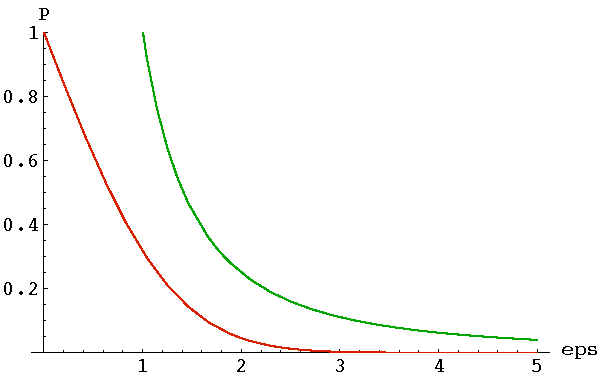
\includegraphics[width=0.8\hsize]{graphics/abwnorm}
\end{center}
\caption{Vergleich der Wahrscheinlichkeit f"ur eine grosse Abweichung
f"ur die Normalverteilung (rot) und die Schranke von Tschebyscheff (gr"un)
\label{abweichung-normalverteilung}}
\end{figure}

Auch f"ur die Normalverteilung wollen wir die Wahrscheinlichkeit
f"ur grosse Abweichungen berechnen. Es gilt wieder
\[
P(|X-\mu|>\varepsilon)
=1-\int_{-\varepsilon}^{\varepsilon}e^{-\frac{x^2}{2\sigma^2}}\,dx
=
1-{\textstyle\frac12}(\operatorname{erf}({\textstyle\frac{\varepsilon}{\sigma\sqrt{2}}})-\operatorname{erf}({\textstyle-\frac{\varepsilon}{\sigma\sqrt{2}}}))
=
1-\operatorname{erf}({\textstyle\frac{\varepsilon}{\sigma\sqrt{2}}})
\]
Die Abbildung~\ref{abweichung-normalverteilung} zeigt die Wahrscheinlichkeit
f"ur eine grosse Abweichung vom Mittelwert ein Einheiten
von $\sqrt{\operatorname{var}(X)}$. Noch deutlicher als bei der
Exponentialverteilung zeigt sich, dass die zus"atzliche Information
"uber die Verteilung die Wahrscheinlichkeit f"ur eine grosse
Abweichung deutlich besser absch"atzen l"asst.

\subsubsection{Der zentrale Grenzwertsatz}
\index{Zentraler Grenzwertsatz}
\index{Grenzwertsatz, zentraler}
\index{Normalapproximation}
In vielen Anwendunge sieht man die Zufallsprozesse nicht einzeln, sondern
man sieht eine grosse Zahl von Zufallsprozessen, die zusammenwirken.
So entsteht der Druck, den ein Gas auf die Wand seines Beh"alters aus"ubt,
durch die grosse Zahl von unabh"angigen St"ossen der einzelnen Gasteilchen
auf die Wand. Das Rauschen in einer elektrischen Schaltung setzt sich
zusammen aus vielen einzelnen Beitr"agen, die zum Beispiel in einzelnen
Bauteilen entstehen, und dort durch das Zusammenspiel der zuf"alligen
thermischen Bewegung der Atome hervorgerufen werden.
Dieses Zusammenspiel von vielen kleinen Zufallsfaktoren soll in diesem
Abschnitt modelliert werden.

Wir gehen dazu von einer Folge von unabh"angigen Zufallsvariablen
\[
X_1,X_2,X_3,\dots
\]
aus, die alle Erwartungswert $0$ und Varianz $1$ haben, also
\[
E(X_i)=0\quad\wedge\quad\operatorname{var}(X_i)=1\qquad\forall i.
\]
Aus diesen Zufallsvariablen werden nun neue Zufallsvariablen
\[
S_n=\frac{X_1+\dots+X_n}{\sqrt{n}}
\]
gebildet, welche wiederum Erwartungswert $0$ und Varianz $1$ haben,
weil
\[
\operatorname{var}(S_n)=\operatorname{var}\bigl(\frac1{\sqrt{n}}(X_1+\dots+X_n)\big)
=\frac1n\operatorname{var}(X_1+\dots+X_n)
\]
ist. Die Summe $S_n$ beschreibt das Zusammenwirken der ersten $n$
Zufallsvariablen $X_i$. Die einzelnen Faktoren k"onnen "ublicherweise
nicht beobachtet werden, nur $S_n$ ist der Messung zug"anglich.

In der Physik lernt man, dass man die st"andige, zufallsbestimmte
Bewegung der Atome in einem Gas oder K"orper nicht im Detail
zu verstehen braucht, und trotzdem eine n"utzliche W"armelehre
aufstellen kann. Daher sollte es m"oglich sein, "uber die Verteilung
$S_n$ mindestens f"ur sehr grosse $n$ etwas auszusagen, selbst
wenn "uber die einzelnen Beitr"age $X_i$ nur sehr wenig bekannt ist.
\begin{figure}
\begin{center}
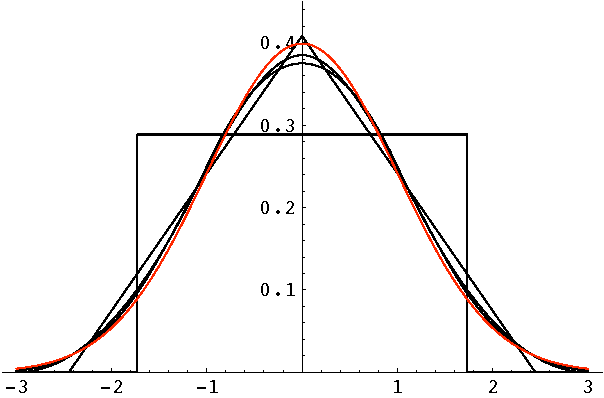
\includegraphics[width=0.8\hsize]{graphics/zgws}
\end{center}
\caption{Zum zentralen Grenzwertsatz: die Wahrscheinlichkeitsdichte
der standardisierten Summe von bis zu vier im Interval
$[-\sqrt{3},\sqrt{3}]$ gleichverteilten Zufallsvariablen (schwarze Kurven)
konvergiert gegen die Standardnormalverteilung (rot).\label{zgws}}
\end{figure}

Der zentrale Grenzwertsatz besagt nun, dass die Verteilungsfunktionen
von $S_n$ gegen die Verteilungsfunktion einer Normalverteilung
konvergieren\footnote{Wie genau diese Konvergenz gemeint ist, wird
im Laufe der Berechnung klar werden.}. In den folgenden Abschnitten
versuchen wir, die Verteilungsfunktion von $S_n$ und insbesondere
ihren Grenzwert zu berechnen. Die Abbildung \ref{zgws} illustriert
dies: dort wird die Wahrscheinlichkeitsdichte der standardisierten
Summe von bis zu vier im
Interval $[-\sqrt{3},\sqrt{3}]$ gleichverteilte Zufallsvariablen dargestellt,
und mit der Standardnormallverteilung verglichen.

Wir betrachten als technisches Hilfsmittel f"ur die Berechnung
die folgende Funktion:
\index{momenterzeugende Funktion}
\begin{definition} Ist $X$ eine Zufallsvariable, dann heisst die Funktion
\marginpar{\raggedright\tiny momenterzeugende Funktion}
\[
M_X(t)=t\mapsto E(e^{tX})=\sum_{k=0}^n\frac{t^k}{k!}E(X^k).
\]
die momenterzeugende Funktion von $X$
\end{definition}
Wir nehmen im folgenden
an, dass diese Funktion existiert\footnote{F"ur alle in diesem Kapitel
untersuchten Verteilungen trifft dies zu, es gibt aber auch Verteilungen,
f"ur die die momenterzeugende Funktion nicht existiert, f"ur die der
zentrale Grenzwertsatz aber trotzdem gilt.}. F"ur die momenterzeugende
\marginpar{\raggedright\tiny Rechenregeln f"ur die momenterzeugende Funktion}
Funktion gilt die folgende Rechenregeln
\begin{eqnarray*}
M_{X+Y}(t)&=&M_X(t)M_Y(t)\\
M_{\lambda X}(t)&=&M_X(\lambda t)
\end{eqnarray*}

Wenn $\varphi$ die Dichtefunktion zur Zufallsvariable $X$ ist, dann
kann die momenterzeugende Funktion wie folgt berechnet werden:
\[
M_X(t)=E(e^{tX})=\int_{-\infty}^\infty e^{tx}\varphi(x)\,dx,
\]
die momenterzeugende Funktion ist also nichts anderes als eine
zweiseitige Laplacetransformierte von $\varphi$:
\[
M_X(t)={\cal L}\varphi(-t),
\]
insbesondere l"asst sich in vielen F"allen aus der Laplacetransformierten
die urspr"ungliche Funktion wieder bestimmen.
Der Plan ist daher der folgende:
\begin{enumerate}
\item Bestimme einen N"aherungsausdruck f"ur $M_{X_i}(t)$.
\item Bestimme einen N"aherungsausdruck f"ur $M_{S_n}(t)$.
\item Berechne den Grenzwert von $M_{S_n}(t)$ f"ur $n\to\infty$.
\item Finde eine Verteilung, die die gleiche Laplacetransformation
hat.
\end{enumerate}

{\parindent0pt\bf 1.~Schritt: N"aherung f"ur $M_{X_i}(t)$.} 
\index{Taylorreihe}
Aus der Taylorentwicklung von $e^{tX}$ folgt
\[
M_{X_i}(t)=1+E(X)t+\operatorname{var}(X)\frac{t^2}{2!}+R_i(t)t^2
=1+\frac{t^2}{2!}+R_i(t)t^2
\]
Dabei ist das Restglied $R_i(t)$ so beschaffen, dass
$R_i(t)\to 0$ wenn $t\to 0$.

\medskip
{\parindent0pt\bf 2.~Schritt: Berechnung von $M_{S_n}(t)$.}
Aus den beiden Rechenregeln f"ur die momenterzeugende Funktion folgt
jetzt zun"achst f"ur die Summe der Zufallsvariablen
\[
M_{X_1+\dots+X_n}(t)=M_{X_1}(t)\dots M_{X_n}(t),
\]
und anschliessen f"ur das Produkt mit $\frac1{\sqrt{n}}$
\[
M_{S_n}(t)=M_{X_1}(t/\sqrt{n})\dots M_{X_n}(t/\sqrt{n}).
\]
Durch Einsetzen der N"aherung aus dem ersten Schritt ergibt sich
\[
M_{S_n}(t)
=\prod_{i=1}^n\biggl(1+\frac{t^2}{2n}+R_i\biggl(\frac{t}{\sqrt{n}}\biggl)\frac{t^2}{n}\biggr)
=\biggl(1+\frac{t^2}{2n}+Q_n\biggl(\frac{t}{\sqrt{n}}\biggr)\frac{t^2}{n}\biggr)^n,
\]
wobei $Q_n(t)$ eine neue Funktion ist. Diese kann durch
\[
Q_n(t/\sqrt{n})=\root{n}\of{M_{S_n}(t)}-1-\frac{t^2}{2n}
\]
ermittelt werden, und hat immer noch die Eigenschaft,
$\lim_{t\to0}Q_n(t)=0$. Im einfachsten Fall, wenn die Zufallsvariablen
identisch verteilt sind, sind alle Funktionen $R_i$ gleich, und damit
auch alle $Q_n$.

\medskip
{\parindent0pt\bf 3.~Schritt: Grenzwert f"ur $n\to\infty$.}
F"ur den Grenz"ubergang $n\to\infty$ beachten wir nun, schreiben wir
$M_{S_n}(t)$ mit Hilfe von
$x_n=\frac{t^2}2+Q_n(t)$
um als
\[
M_{S_n}(t)=\biggl(1+\frac{x_n}n\biggr)^n
\]
Nun ist bereits aus der Analysis bekannt, dass
\[
\lim_{n\to\infty}\biggl(1+\frac{x}{n}\biggr)^n=e^x,
\]
es gilt aber auch in verallgemeinerter Form:
\[
\biggl(1+\frac{x_n}{n}\biggr)^n\to e^x\quad\text{falls}\quad x_n\to x.
\]
Da in unserem Fall $x_n\to \frac{t^2}2$ erhalten wir
\[
\lim_{n\to\infty}M_{S_n}(t)=e^{\frac{t^2}{2}}
\]

\medskip
{\parindent0pt\bf 4.~Schritt: Die Grenzverteilung.}
Der gefundene Grenzwert soll die momenterzeugende Funktion einer
Verteilung sein, und wir erwarten, dass sie ebenfalls eine
momenterzeugende Funktion hat. Da die momenterzeugende Funktion
nichts anderes als eine Laplacetransformation ist, k"onnen wir
den Eindeutigkeitssatz f"ur die Laplacetransformation anwenden,
welcher besagt, dass zwei Funktionen, die die gleiche zweiseitige
Laplacetransformierte haben, fast "uberall gleich sein.

Wir rechnen nach, dass $e^{\frac{t^2}2}$ die momenterzeugende Funktion
der Standardnormalverteilung ist. Wir berechnen
dazu die Momente der Normalverteilung $\frac1{\sqrt{2\pi}}e^{-\frac{x^2}2}$
\begin{eqnarray*}
\int_{-\infty}^\infty e^{-\frac{x^2}2}x^{2k+1}\,dx&=&0\\
\int_{-\infty}^\infty e^{-\frac{x^2}2}x^{2k}\,dx
&=&
\biggl[\frac{x^{2k+1}}{2k+1}e^{-\frac{x^2}2}\biggr]_{-\infty}^\infty
+\frac1{(2k+1)}\int_{-\infty}^\infty x^{2k+2}e^{-\frac{x^2}2}\,dx\\
&=&
\frac1{(2k+1)}\int_{-\infty}^\infty x^{2k+2}e^{-\frac{x^2}2}\,dx
\end{eqnarray*}
Insbesondere kann man das $2k+2$-te Moment mit Hilfe einer
Rekursionsformel aus dem $2k$-ten Moment berechnen:
\[
E(X^{2k+2})=(2k+1)E(X^{2k}).
\]
Das $2k$-te Moment ist die Varianz, also $E(X^2)=1$. Damit kann
man die momenterzeugende Funktion von $e^{-\frac{x^2}2}$ aufschreiben:
\begin{eqnarray*}
M(t)
&=&
1+\frac{t^2}{2!} +\frac{t^4}{4!}3 +\frac{t^6}{6!}3\cdot5 +\frac{t^8}{8!}3\cdot5\cdot7+\dots\\
&=&
1+\frac{t^2}{1!\cdot 2^1} +\frac{t^4}{2! \cdot 2^2} +\frac{t^6}{3!\cdot 2^3}
+\frac{t^8}{4!\cdot 2^4}\\
&=&
1+(t^2/2) +\frac{(t^2/2)^2}{2!} +\frac{(t^2/2)^3}{3!}
+\frac{(t^2/2)^4}{4!}\\
&=&e^{\frac{t^2}2}
\end{eqnarray*}
Mit anderen Worten, die momenterzeugende Funktion der Normalverteilung
stimmt "uberein mit der momenterzeugenden Funktion der Grenzverteilung.
Schreiben $\varphi_n$ f"ur die Dichtefunktion f"ur $S_n$ und $F_n$
f"ur die Verteilungsfunktion, dann gilt
nach allgemeinen S"atzen "uber die Laplacetransformation gilt daher
\[
\lim_{n\to\infty}\varphi_n(x)=\frac1{\sqrt{2\pi}}e^{-\frac{x^2}2}
\quad\text{fast "uberall}
\]
und f"ur die Verteilungsfunktion
\[
\lim_{n\to\infty}F_n(x)=\frac1{\sqrt{2\pi}}\int_{-\infty}^xe^{-\frac{t^2}2}\,dt
\]
Insgesamt haben wir damit den folgenden Satz bewiesen
\begin{satz}[Zentraler Grenzwertsatz]
Sind $(X_i)_{1\le i}$ unabh"angige Zufallsvariable mit
Erwartungswert $E(X_i)=0$ und Varianz $\operatorname{var}(X_i)=1$
f"ur alle $i\ge 1$. Dann ist
\[
S_n=\frac1{\sqrt{n}}\sum_{i=1}^nX_i=\frac1{\sqrt{n}}(X_1+\dots+X_n)
\]
eine Folge von Zufallsvariablen, die ebenfalls Erwartungswert $E(S_n)=0$
und Varianz $\operatorname{var}(S_n)=1$ haben. Falls die Zufallsvariablen
$X_i$
f"ur alle $i$ eine momenterzeugende Funktion haben, hat auch $S_n$
f"ur alle $n$ eine momenterzeugende Funktion, ausserdem konvergiert
die Verteilungsfunktion $F_n$ von $S_n$ gegen die Verteilungsfunktion der
Standardnormalverteilung
\[
\lim_{n\to\infty}F_n(x)=\frac1{\sqrt{2\pi}}\int_{-\infty}^xe^{-\frac{t^2}2}\,dt.
\]
Haben die $X_i$ ausserdem eine Wahrscheinlichkeitsdichte,
dann hat auch $S_n$
die Wahrscheinlichkeitsdichte $\varphi_n$, welche fast "uberall gegen die
Wahrscheinlichkeitsdichte der Standardnormalverteilung 
konvergiert:
\[
\lim_{n\to\infty}\varphi_n(x)=\frac1{\sqrt{2\pi}}e^{-\frac{x^2}2}.
\]
\end{satz}

\subsection{$\chi^2$-Verteilung\label{chi2verteilung}}
\index{chi@{$\chi^2$-Verteilung}}
Der zentrale Grenzwertsatz garantiert, dass in vielen praktisch wichtigen
F"allen ann"ahernd normalverteilte Zufallsvariablen vorliegen.
Wenn man nun also weiss, dass die Zufallsvariablen $(X_i)_{1\le i\le n}$
mit Erwartungswert $\mu_i$ und Varianz $\sigma_i^2$ normalverteilt
sind, dann sind die Zufallsvariablen $Y_i=(X_i-\mu_i)/\sigma_i$
standardnormalverteilt. Die meisten $Y_i$ werden also Werte nahe
bei $0$ annehmen, die Summe $\sum_{i=1}^nY_i^2$ wird also im
Allgemeinen klein sein. Grosse Werte der Summe sind sehr unwahrscheinlich.
Treten sie bei einer Beobachtung trotzdem auf, dann ist entweder genau
dieser unwahrscheinliche Fall eingetreten, oder die Annahmen, dass die
$X_i$ normalverteilt waren, ist nicht zutreffend. Somit l"asst sich
aus der Gr"osse ein praktisch n"utzlicher Test konstruieren, ob
eine Normalverteilung vorliegt.

\begin{definition}
Sind $(X_i)_{1\le i\le n}$ standardnormalverteilte Zufallsvariable,
dann ist $\sum_{i=1}^nX_i^2$ eine $\chi^2$-verteilte Zufallsvariable
mit $n$ Freiheitsgraden.
\end{definition}

\begin{satz}\label{chi2}
Die $\chi^2$-Verteilung mit $n$ Freiheitsgraden hat
die Wahrscheinlichkeitsdichte
\[
\gamma_{\frac12,\frac{n}2}(x)=\frac1{\Gamma(\frac{n}2)}\sqrt{\frac1{2^n}x^{n-2}}e^{-\frac12x}\qquad,x\ge 0
\]
Die momenterzeugende Funktion der $\chi^2$-Verteilung ist
\[
\chi_n^2(t)=(1-2t)^{-\frac{n}2}.
\]
\end{satz}

Um diesen Satz zu beweisen, ist es n"utzlich, mehr Information "uber die
Dichtefunktionen zu sammeln. Zun"achst sind die Dichtefunktionen
$\gamma_{\frac12,\frac{n}2}$ Elemente einer viel gr"osseren Familie von
Dichtefunktionen, n"amlich den Gamma-Verteilungen

\subsubsection{Die Gamma-Verteilungen}
\index{gamma@{$\gamma$-Verteilung}}
\begin{definition}
Die Verteilung mit der Dichtefunktion
\[
\gamma_{\alpha,\nu}(x)=\begin{cases}
\displaystyle \frac1{\Gamma(\nu)}\alpha^\nu x^{\nu-1}e^{-\alpha x}&\qquad x>0\\
0&\qquad\text{sonst}
\end{cases}
\]
heist Gamma-Verteilung zum Parameter $(\alpha,\nu)$. Darin ist
\[
\Gamma(t)=\int_0^\infty x^{t-1}e^{-x}\,dx
\]
die Gamma-Funktion.
\end{definition}

Die Gamma-Verteilungen erf"ullen einige interessante Rechenregeln:
\begin{satz} Die Funktionen $\gamma_{\alpha,\nu}$ sind Wahrscheinlichkeitsdichten.
Die Gamma-Verteilungen sind unter Faltung abgeschlossen:
\[
\gamma_{\alpha,\mu}*\gamma_{\alpha,\nu}=\gamma_{\alpha,\mu+\nu}.
\]
Sind $X$ und $Y$ Gamma-verteilte Zufallsvariable, dann ist auch $X+Y$
Gamma-verteilt.
\end{satz}
\begin{proof}[Beweis]
Wir rechnen zun"achst nach, dass $\gamma_{\alpha,\nu}$ tats"achlich
Wahrscheinlichkeitsdichten sind. Dazu ist die Normierung zu pr"ufen:
\begin{eqnarray*}
\int_{-\infty}^\infty \gamma_{\alpha,\nu}(x)\,dx
&=&\int_0^\infty\frac1{\Gamma(\nu)}\alpha^\nu x^{\nu-1}e^{-\alpha x}\,dx\\
&=&\frac{1}{\Gamma(\nu)}\int_0^\infty (\alpha x)^{\nu-1}e^{-\alpha x}
\alpha\,dx\\
&=&\frac1{\Gamma(\nu)}\int_0^\infty \xi^{\nu-1}e^{-\xi}\,d\xi=1
\end{eqnarray*}
Die letzte Gleichung folgt aus der Definition der Gamma-Funktion.

Wir berechnen jetzt das Faltungsprodukt von $\gamma_{\alpha,\mu}$ und
$\gamma_{\alpha,\nu}$, wir wissen bereits, dass das Faltungsprodukt wieder
eine Wahrscheinlichkeitsdichte sein wird. Es gilt
\begin{eqnarray*}
\gamma_{\alpha,\mu}*\gamma_{\alpha,\nu}(x)
&=&\int_{-\infty}^\infty \gamma_{\alpha,\mu}(x-t)\gamma_{\alpha,\nu}(t)\,dt\\
&=&\int_0^x \gamma_{\alpha,\mu}(x-t)\gamma_{\alpha,\nu}(t)\,dt\\
&=&\int_0^x \frac1{\Gamma(\mu)}\alpha^{\mu}(x-t)^{\mu-1}e^{-\alpha (x-t)}
\frac1{\Gamma(\nu)}\alpha^\nu t^{\nu-1}e^{-\alpha t}\,dt\\
&=&\frac{\alpha^{\mu+\nu}e^{-\alpha x}}{\Gamma(\mu)\Gamma(\nu)}\int_0^x
(x-t)^{\mu-1}t^{\nu-1}\,dt\\
&=&\frac{\alpha^{\mu+\nu}e^{-\alpha x}}{\Gamma(\mu)\Gamma(\nu)}x^{\mu+\nu-1}
\int_0^1 (1-\tau)^{\mu-1}\tau^{\nu-1}\,d\tau\\
&=&
\frac1{\Gamma(\mu+\nu)}\alpha^{\mu+\nu}e^{-\alpha x}
x^{\mu+\nu-1}
\cdot
\frac{\Gamma(\mu+\nu)}{\Gamma(\mu)\Gamma(\nu)}
\int_0^1 (1-\tau)^{\mu-1}\tau^{\nu-1}\,d\tau\\
&=&\gamma_{\alpha,\mu+\nu}
\cdot
\frac{\Gamma(\mu+\nu)}{\Gamma(\mu)\Gamma(\nu)}
\int_0^1 (1-\tau)^{\mu-1}\tau^{\nu-1}\,d\tau
\end{eqnarray*}
wobei f"ur die Umformung des Integrals die Substitution $t=x\tau$ verwendet
wurde. Somit ist das Faltungsprodukt bis auf eine konstanten Faktor
wieder eine Gamma-Verteilung, da aber die Gamma-Verteilungen bereits
normiert sind, muss der Faktor eins sein. Als Nebenprodukt erhalten
wir also die Formel
\[
\int_0^1(1-t)^{\mu-1}t^{\nu-1}\,dt=\frac{\Gamma(\mu)\Gamma(\nu)}{\Gamma(\mu+\nu)}.
\]
\end{proof}

\subsubsection{Beweis des Satzes \ref{chi2}}
Die $\chi^2$-Verteilung mit einem Freiheitsgrad ist die Verteilung von
$X^2$, wenn $X$ eine standardnormalverteilte Zufallsvariable ist.
F"ur $x\le 0$ ist die Verteilungsfunktion $F(x)=P(X^2\le x)=0$. 
F"ur $x>0$ gilt
\begin{eqnarray*}
F(x)&=&P(X^2\le x)=P(-\sqrt{x}\le X\le\sqrt{x})\\
&=&\frac1{\sqrt{2\pi}}\int_{-\sqrt{x}}^{\sqrt{x}}e^{-\frac12 \xi^2}\,d\xi\\
&=&\sqrt{\frac{2}{\pi}}\int_0^{\sqrt{x}}e^{-\frac12\xi^2}\,d\xi
\end{eqnarray*}
Mit Hilfe der Substitution $\xi^2=t$ oder $\xi=t^{\frac12}$ k"onnen wir
dies umformen zu
\begin{eqnarray*}
F(x)&=&\frac1{\sqrt{2\pi}}\int_0^xe^{-\frac12t}t^{-\frac12}\,dt\\
&=&\frac1{\sqrt{2\pi}}\int_0^x\gamma_{\frac12,\frac12}(t)
\frac{\Gamma(\frac12)}{{\frac12}^{\frac12}}\,dt
\end{eqnarray*}
Die Ableitung nach $x$ ergibt die Dichtefunktion:
\[
\varphi(x)=\frac1{\sqrt{\pi}}\Gamma({\textstyle\frac12})\gamma_{\frac12,\frac12}(x)
\]
Der Wert der Gamma-Funktion ist
\[
\Gamma({\textstyle\frac12})
=\int_0^\infty x^{-\frac12}e^{-x}\,dx
\]
kann mit der Substitution $x=\xi^2$ berechnet werden,
\[
\Gamma({\textstyle\frac12})=\int_0^\infty \xi^{-1}e^{-\xi^2}2\xi\,d\xi
=\int_0^{\infty}e^{-\xi^2}\,d\xi
\]
Das Integral auf der echten Seite ist bis auf einen Normierungsfaktor
das Integral "uber die Dichte einer Normalverteilung, also
\[
\Gamma({\textstyle\frac12})=\sqrt{\pi},
\]
woraus sich ablesen l"asst, dass die Wahrscheinlichkeitsdichte 
von $X^2$ tats"achlich $\gamma_{\frac12,\frac12}$ ist.

Nun kann man vollst"andige Induktion zusammen mit der Faltungseigenschaft
verwenden. F"ur $n=1$ ist bereits bekannt, dass die Wahrscheinlichkeitsdichte
f"ur $n$ Summanden $X_i^2$ $\gamma_{\frac12,\frac{n}2}$ ist. Nehmen wir an,
dass f"ur $n-1$ Summanden die Wahrscheinlichkeitsdichte
$\gamma_{\frac12,\frac{n-1}2}$
ist, dann erhalten wir f"ur $n$ Summanden mit der Faltungseigenschaft
\[
\gamma_{\frac12,\frac12}*\gamma_{\frac12,\frac{n-1}2}=\gamma_{\frac12,\frac{n}2}.
\]

Es bleibt, die momenterzeugende Funktion von $\chi_n^2$ zu berechnen.
Wegen
\[
M_{\chi_{n-1}^2}(t)M_{\chi_1^2}(t)=M_{\chi_n^2}(t)
\]
gen"ugt es, eine Formel f"ur $M_{\chi_1^2}(t)$ zu finden. Die Dichte
der $\chi_1^2$-Verteilung ist
\[
\frac1{\sqrt{2\pi}}e^{-\frac{x}2}x^{-\frac12}.
\]
Nach Definition der momenterzeugenden Funktion ist
\begin{eqnarray*}
M_{\chi_1^2}(t)
&=&\frac1{\sqrt{2\pi}}\int_0^\infty e^{xt}e^{-\frac{x}2}x^{-\frac12}\,dx\\
&=&\frac1{\sqrt{2\pi}}\int_0^\infty x^{-\frac12}e^{x(t-\frac12)}\,dx\\
&=&\frac1{\sqrt{2\pi}}\int_0^\infty x^{-\frac12}e^{-\alpha x}\,dx\\
&=&\frac1{\sqrt{2\pi}}\frac1{\sqrt{\alpha}}\int_0^\infty\xi^{-\frac12}e^{-\xi}\,d\xi\\
&=&\frac1{\sqrt{2\pi}}\frac1{\alpha}\Gamma(\frac12)=\frac1{2\alpha}\\
&=&\frac1{\sqrt{1-2t}}=(1-2t)^{-\frac12},
\end{eqnarray*}
wobei wir die Subsitutionen $-\alpha=t-\frac12$ und $\alpha x=\xi$
verwendet haben. Somit ist
\[
M_{\chi_1^2}(t)=(1-2t)^{-\frac12},
\]
also auch
\[
M_{\chi_n^2}(t)=(1-2t)^{-\frac{n}2}.
\]
Damit der Satz \ref{chi2} vollst"andig bewiesen ist.

\subsubsection{Normalverteilungstest}
\index{Normalverteilungstest}
Die Zufallsvariablen $X_i$ waren unabh"angig und standardnormalverteilt
vorausgesetzt worden.
Die Gr"osse $\sum_{i=1}^nX_i^2$ liefert einen Test daf"ur, ob die Gr"ossen
$X_i$ tats"achlich standardnormalverteilt sind. Ist zum Beispiel der
Erwartungswert der $X_i$ nicht $0$, dann wird $\sum_{i=1}^nX_i^2$
deutlich gr"osser. Die Hypothese, dass die $X_i$ standardnormalverteilt
sind, kann also verworfen werden, wenn $\sum_{i=1}^nX_i^2$ eine gewisse
Schranke $M$ "uberschreitet. Die Wahrscheinlichkeit, dass die Hypothese
verworfen wird, obwohl sie eigentlich zutrifft, ist
\[
P(\sum_{i=1}^nX_i^2>M).
\]
Will man die Wahrscheinlichkeit eines solchen Irrtums klein halten, muss
$M$ entsprechend gross gew"ahlt werden. Wie gross definiert die
$\chi^2$-Verteilung. Soll die Fehlerwahrscheinlichkeit $p$ sein,
dann muss $M$ so gew"ahlt werden, dass 
\[
P(\sum_{i=1}^nX_i^2>M)=\int_M^\infty \gamma_{\frac12,\frac{n}2}(t)\,dt = p.
\]
Die Schranke $M$ ist f"ur verschiedene Werte von $p$ in Abh"angigkeit
von der Anzahl Freiheitsgrade tabelliert, oder kann mit dem Computer
berechnet werden.
Zu diesem Zweck ist zum Beispiel in der GNU Scientific
Library die Funktion \verb+gsl_cdf_chisq_Pinv(double p, double nu)+
vorhanden, der Parameter \verb+p+ ist die Wahrscheinlichkeit eines
Fehlers, {\tt nu} ist die Zahl der Freiheitsgrade.

\subsection{Potenzgesetze}
Die Normalverteilung beschreibt physikalische Gr"ossen sehr erfolgreich,
die vor allem in einer bestimmten Gr"osse vorkommen. Menschen sind zum
Beispiel im Durchschnitt etwa 1.80m gross, Abweichungen kommen vor, sind
aber sehr selten, 5m grosse Menschen gibt es nicht.

Andererseits gibt es auch Gr"ossen, die einen weiten Bereich von m"oglichen
Werten annehmen. Mondkrater k"onnen mehrere Kilometer gross sein, oder auch
nur ein paar Milimeter. Der Entstehungsmechanismus ist unabh"angig von der
Gr"ossenskala immer der Selbe. Diese Unabh"angigkeit von der Gr"ossenskala
sollte sich auch in der Verteilungsfunktion der Gr"osse niederschlagen.
In diesem Abschnitt sollen die Eigenschaften solcher Verteilungen abgeleitet
werden.

\subsubsection{Skalenunabh"angigkeit und Potenzgesetze}
Wir untersuchen nun Zufallsvariablen $X$ wie zum Beispiel den Durchmesser
von Mondkratern. 
Die Verteilung soll also f"ur jeden beliebigen
Mass\-stab gelten. Die Form des Graphen von $\varphi(x)$ darf sich nicht "andern,
wenn wir zu einer anderen Skala "ubergehen.
F"ur jede Zahl $b>0$ muss es also eine Konstante $g(b)$ geben, 
so dass
$$\varphi(bx)=g(b)\varphi(x).$$
Aus diesem Zusammenhang folgt sofort, dass
$\varphi(b)=g(b)\varphi(1)$ und weiter 
$$\varphi(bx)=\frac{\varphi(b)\varphi(x)}{p(1)}.$$
Leitet man dies nach $b$ ab und setzt $b=1$ erh"alt man
\begin{align*}
x\varphi'(bx)&=\frac{\varphi'(1)p(x)}{\varphi(1)}\\
x\varphi'(x)&=\frac{\varphi'(1)}{\varphi(1)}\varphi(x)
\end{align*}
Dies ist eine gew"ohnliche lineare Differentialgleichung
erster Ordnung, die man mit Separation der Variablen
l"osen kann
\begin{align*}
\frac{\varphi'(x)}{\varphi(x)}&=\frac{\varphi'(1)}{\varphi(1)}\frac1x
\\
\int\frac{\varphi'(x)}{\varphi(x)}\,dx&=\frac{\varphi'(1)}{\varphi(1)}\int\frac{dx}x + c
\\
\log \varphi(x)&=\frac{\varphi'(1)}{\varphi(1)}\log x+c
\\
\varphi(x)&=Cx^{-\alpha}\qquad\text{mit $\alpha=-\frac{\varphi'(1)}{\varphi(1)}$}
\end{align*}
Der Exponent $-\alpha$ ist immer negativ da $\varphi'(1)<0$ sein muss.

\begin{definition}
Eine Verteilung mit der Dichtefunktion
$$\varphi(x)=\begin{cases}
Cx^{-\alpha}&\qquad x>x_{\min}\\
0&\qquad\text{sonst}
\end{cases}
$$
heisst Potenzgesetz.
\end{definition}
Damit dies eine Wahrscheinlichkeitsverteilung definiert, muss $C$
so gew"ahlt werden, dass das Integral "uber $\mathbb R$ den Wert $1$
ergibt,
\begin{align*}
1=\int_{-\infty}^\infty\varphi(x)\,dx
&=
\int_{x_{\min}}^\infty Cx^{-\alpha}\,dx
\\
&=
\left[-\frac{C}{1-\alpha}x^{1-\alpha}\right]_{x_{\min}}^\infty
\\
&=
C\frac{x_{\min}^{1-\alpha}}{1-\alpha}
\\
\Rightarrow\qquad
C
&=
\frac{\alpha-1}{x_{\min}^{1-\alpha}}
\end{align*}
Die Berechnung der Normierungskonstanten zeigt auch, dass die Normierung
f"ur $\alpha \le 1$ nicht mehr m"oglich ist, Potenzgesetze sind daher
nur f"ur $\alpha > 1$ m"oglich.

\begin{satz}
Die Dichtefunktion einer nach einem Potenzgesetz verteilten Zufallsvariablen
ist 
$$\varphi(x)=\begin{cases}
\displaystyle
\frac{\alpha-1}{x_{\min}^{1-\alpha}}
x^{-\alpha}&\qquad x>x_{\min}
\\
0&\qquad\text{sonst},
\end{cases}
$$
wobei $\alpha>1$ gelten muss.
\end{satz}

Nach einem Potenzgesetz verteilte Zufallsvariablen kann man daran
erkennen, dass die Dichtefunktion in einer doppelt logarithmischen
Darstellung eine Gerade ist. Wegen
$$\log p(x)=-\alpha \log x+\log C$$
ist die Steigung der Geraden $-\alpha$.

\subsubsection{Erwartungswert und Varianz}
Mit Hilfe der Dichtefunktion k"onnen die "ublichen Kennzahlen der Verteilung
berechnet werden.
Der Erwartungswert einer nach einem Potenzgesetz verteilten Zufallsvariable $X$
ist
\begin{align*}
E(X)&=
\int_{-\infty}^\infty x\varphi(x)\,dx
\\
&=
\int_{x_{\min}}^\infty 
x
\frac{\alpha-1}{x_{\min}^{1-\alpha}}
x^{-\alpha}\,dx
\\
&=
\frac{\alpha-1}{x_{\min}^{1-\alpha}}
\left[\frac{1}{2-\alpha}x^{2-\alpha}\right]_{x_{\min}}^\infty
\\
&=
\frac{\alpha-1}{\alpha-2}x_{\min}
\end{align*}
Dies ist nat"urlich nur m"oglich, solange $\alpha > 2$.

F"ur die Varianz berechnet man zun"achst das zweite Moment
\begin{align*}
E(X^2)&=
\int_{-\infty}^\infty x^2\varphi(x)\,dx
\\
&=
\int_{x_{\min}}^\infty 
x^2
\frac{\alpha-1}{x_{\min}^{1-\alpha}}
x^{-\alpha}\,dx
\\
&=
\frac{\alpha-1}{\alpha-1}\frac1{x_{\min}^{1-\alpha}}\left[-x^{3-\alpha}\right]_{x_{\min}}^\infty
\\
&=
\frac{\alpha-1}{\alpha-3}x_{\min}^2
\end{align*}
Dieses Moment existiert also nur, wenn $\alpha >3$. Die Varianz wird damit
\begin{align*}
\operatorname{var}(X)
&=
E(X^2)-E(X)^2
\\
&=
\biggl(
\frac{\alpha-1}{\alpha-3}-\biggl(\frac{\alpha-1}{\alpha-2}\biggr)^2
\biggr)x_{\min}^2
\end{align*}
\begin{satz}
Ist $X$ verteilt nach einem Potenzgesetz mit Exponent $\alpha$, dann
existiert f"ur $\alpha>2$ ein Erwartungswert
$$
E(X)
=
\frac{\alpha-1}{\alpha-2}x_{\min}
$$
und f"ur $\alpha >3$ auch eine Varianz
$$
\operatorname{var}(X)
=
\biggl(
\frac{\alpha-1}{\alpha-3}-\biggl(\frac{\alpha-1}{\alpha-2}\biggr)^2
\biggr)x_{\min}^2
$$
\end{satz}

\subsubsection{Median}
Der Median ist derjenige Wert $x_{\frac12}$ der Zufallsvariablen,
f"ur den die Verteilungsfunktion den Wert $\frac12$ annimmt, also
\begin{align*}
\frac12=\int_{-\infty}^{x_{\frac12}}\varphi(x)\,dx
&=
\int_{x_{\min}}^{x_{\frac12}}
\frac{\alpha-1}{x_{\min}^{1-\alpha}}
x^{-\alpha}\,dx
\\
&=
\frac{\alpha-1}{x_{\min}^{1-\alpha}}\left[
\frac{x^{1-\alpha}}{1-\alpha}
\right]_{x_{\min}}^{x_{\frac12}}
\\
&=
\frac{x_{\min}^{1-\alpha}-x_{\frac12}^{1-\alpha}}{x_{\min}^{1-\alpha}}
\\
&=
1-\left(
\frac{x_{\frac12}}{x_{\min}}
\right)^{1-\alpha}
\end{align*}
Diese Gleichung kann man nach $x_{\frac12}$ aufl"osen:
\begin{align*}
\frac{x_{\frac12}}{x_{\min}}
&=
\left(\frac12\right)^{\frac1{1-\alpha}}
\\
x_{\frac12}&=2^{\frac1{\alpha-1}}x_{\min}
\end{align*}
\begin{satz}
Ist die Zufallsvariable $X$ nach einem Potenzgesetz mit Exponent $\alpha>1$
verteilt, existiert der Median
$$x_{\frac12}=2^{\frac1{\alpha-1}}x_{\min}.$$
\end{satz}

\subsubsection{Die 80/20-Regel}
\begin{figure}
\begin{center}
\includegraphics[width=0.8\hsize]{images/power}
\end{center}
\caption{Kurven $(P(x),W(x))$ f"ur verschiedene Werte von $\alpha$\label{wp}}
\end{figure}
Die 80/20-Regel besagt, dass 20\% der Werte f"ur 80\% des kumulierten Wertes
verantwortlich sind.

Allgemeiner k"onnen wir f"ur jedes $x$ nach der Wahrscheinlichkeit
eines Wertes $>x$ fragen und ihn vergleichen mit dem gesamten Erwartungswert,
den die Werte $>x$ ergeben.
Die Wahrscheinlichkeit eines Wertes $>x$ ist
\begin{align}
P(x)
&=
\int_x^\infty
\frac{\alpha-1}{x_{\min}^{1-\alpha}}
x^{-\alpha}
\,dx
\notag
\\
&=
-\frac{1}{x_{\min}^{1-\alpha}}
\left[x^{1-\alpha}\right]_x^\infty
=
\left(
\frac{x}{x_{\min}}
\right)^{1-\alpha}
\label{px}
\end{align}
Den Beitrag der Werte $>x$ zum Erwartungswert berechnet die Funktion
\begin{equation}
W(x)=\frac%
{\int_x^\infty \xi\varphi(\xi)\,d\xi}%
{\int_{x_{\min}}^\infty \xi\varphi(\xi)\,d\xi}.
\label{wx}
\end{equation}
Nach den bisher durchgef"uhrten Rechnungen ist
$$W(x)=\left(\frac{x}{x_{\min}}\right)^{2-\alpha}
=P(x)^{\frac{\alpha-2}{\alpha-1}}$$
Die Abbildung \ref{wp} zeigt den Zusammenhang zwischen $P(x)$ und $W(x)$
f"ur verschiedene Werte von $\alpha$

Die 80/20-Regel entspricht der Kurve, die durch den 
Punkt mit $P(x)=0.2$ und $W(x)=0.8$ geht, also
\begin{align*}
0.8&=0.2^{\frac{\alpha-2}{\alpha-1}}
\\
\frac{\log 0.8}{\log 0.2}
&=
\frac{\alpha-2}{\alpha-1}
\end{align*}
Schreiben wir f"ur das Verh"altnis der Logarithmen auf der linken
Seite $\lambda$ ergibt sich die Gleichung
\begin{align*}
\lambda
&=
\frac{\alpha-2}{\alpha-1}
\\
\alpha(\lambda-1)&=\lambda-2
\\
\alpha&=\frac{\lambda-2}{\lambda-1}
\end{align*}
Im konkreten Fall ist der numerische Wert f"ur $\alpha=2.160964$.

F"ur $\alpha\le 2$ existieren die Erwartungswerte nicht mehr, die
Integrale in (\ref{wx}) divergieren. Wenn man jedoch
eine gemeinsame obere Schranke $x_{\max}$ verwendet, kann man $P$
und $W$ als von dieser Schranke abh"angige Gr"ossen immer noch
definieren und den Grenzwert f"ur $x_{\max}\to\infty$ erst nachher
durchf"uhren. Dabei stellt sich heraus, dass
\begin{align*}
W(x)
&=
\lim_{x_{\max}\to\infty}
\frac%
{\int_x^{x_{\max}} \xi\varphi(\xi)\,d\xi}%
{\int_{x_{\min}}^{x_{\max}} \xi\varphi(\xi)\,d\xi}.
\\
&=
\lim_{x_{\max}\to\infty}
\frac%
{x_{\max}^{2-\alpha}-x^{2-\alpha}}%
{x_{\max}^{2-\alpha}-x_{\min}^{2-\alpha}}
=1
\end{align*}
Sobald also $\alpha\le2$ ist, sind alle Beitr"age zum Erwartungswert
in einem noch so kleinen Teil der gr"ossten Werte konzentriert.

"Ubersetzt in die aktuelle Diskussion "uber Verm"ogensverteilungen
und Managerl"ohne bedeutet dies, dass f"ur $\alpha\le2$ jeder noch so
kleine Teil der Spitze der Einkommenspyramide alles besitzt, und alle
anderen nichts. Je n"aher $\alpha$ an $1$ kommt desto extremer wird
das Ungleichgewicht zwischen arm und reich.

\subsubsection{Parameter sch"atzen}
Um den Parameter $\alpha$ zu sch"atzen k"onnte man f"ur die Punkte
eines Histogramms eine lineare Regression durchf"uhren.
Eine Maximum-Likelihood-Sch"atzung f"uhrt jedoch direkter zum
Ziel.
Mit der Dichtefunktion
$$\varphi(x)=\frac{\alpha-1}{x_{\min}}\left(\frac{x}{x_{\min}}\right)^{-\alpha}$$
wird die Likelihoodfunktion
$$
L(\alpha;x_1,\dots,x_n)=
\left(\frac{\alpha-1}{x_{\min}}\right)^n
\prod_{i=1}^n
\left(\frac{x_i}{x_{\min}}\right)^{-\alpha}$$
$\alpha$ ist so zu bestimmen, dass $L(\alpha;x_1,\dots,x_n)$ maximal
wird.
Dies ist gleichbedeutend damit, dass der nat"urliche 
Logarithmus $\log L(\alpha;x_1,\dots,x_n)$ maximiert wird.
Partielle Ableitung nach $\alpha$ ergibt
\begin{align*}
\frac{\partial}{\partial \alpha}
L(\alpha;x_1,\dots,x_n)
&=
\frac{\partial}{\partial\alpha}
\biggl[
n\log(\alpha-1)-n\log x_{\min}
-\alpha\biggl( \sum_{i=1}^n\log x_i-n \log x_{\min}\biggr)
\biggr]
\\
&=
\frac{n}{\alpha-1}-\sum_{i=1}^n\log x_i-n\log x_{\min}=0
\end{align*}
Diese Gleichung kann man nach $\alpha$ aufl"osen und findet
\begin{align*}
\frac{n}{\alpha-1}
&=
\sum_{i=1}^n \log\frac{x_i}{x_{\min}}
\\
\alpha&=1+\frac{n}{
\sum_{i=1}^n \log\frac{x_i}{x_{\min}}
}.
\end{align*}



%
% diskrete-verteilungen.tex -- Abschnitt über diskrete Verteilungen
%
% (c) 2006-2015 Prof. Dr. Andreas MŸller
%
\section{Diskrete Wahrscheinlichkeitsverteilungen}
Neben den vielen praktisch wichtigen stetigen Verteilungen
gibt es auch ein mindestens genauso lange Liste bedeutender
diskreter Verteilungen.

%
% dgleichverteilung.tex -- Abschnitt ueber diskrete Gleichverteilung in Kapitel 5
%
% (c) 2015 Prof Dr Andreas Mueller, Hochschule Rapperswil
%
\subsection{Gleichverteilung} \label{section-gleichverteilung-diskret}
\index{Gleichverteilung!Erwartungswert}
\index{Gleichverteilung!Varianz}
\index{Gleichverteilung!Verteilungsfunktion}
\begin{table}
\renewcommand{\arraystretch}{1.5}
\begin{center}
\begin{tabular}{|l|l|}
\hline
Name&diskrete Gleichverteilung\\
\hline
Wahrscheinlichkeit&
\begin{minipage}{3.7in}
\vskip3pt
$\displaystyle P(k)=\frac1n$
\end{minipage}
\\
Verteilungsfunktion&
\begin{minipage}{3.7in}
$\displaystyle
\begin{cases}
0&\qquad x \le 1\\
{\displaystyle \frac{\left\lfloor x\right\rfloor}n}&\qquad 1\le x\le n
\\
1&\qquad x \ge n
\end{cases}
$
\end{minipage}
\\[30pt]
Erwartungswert&$\displaystyle \frac{n+1}2$\\[8pt]
Varianz&$\displaystyle \frac{n^2-1}{12}$\\[8pt]
Median&$\displaystyle \frac{n+1}2$\\[8pt]
\hline
Anwendungen&\begin{minipage}{3.7in}%
\vskip3pt
\strut
$\bullet$ Laplace-Ereignisse aller Art\\
$\bullet$ W"urfel\\
$\bullet$ Roulette
\strut
\end{minipage}\\[17pt]
\hline
\end{tabular}
\end{center}
\caption{Datenblatt der diskreten Gleichverteilung\label{datenblatt:diskretegleichverteilung}}
\end{table}

\begin{figure}
\centering
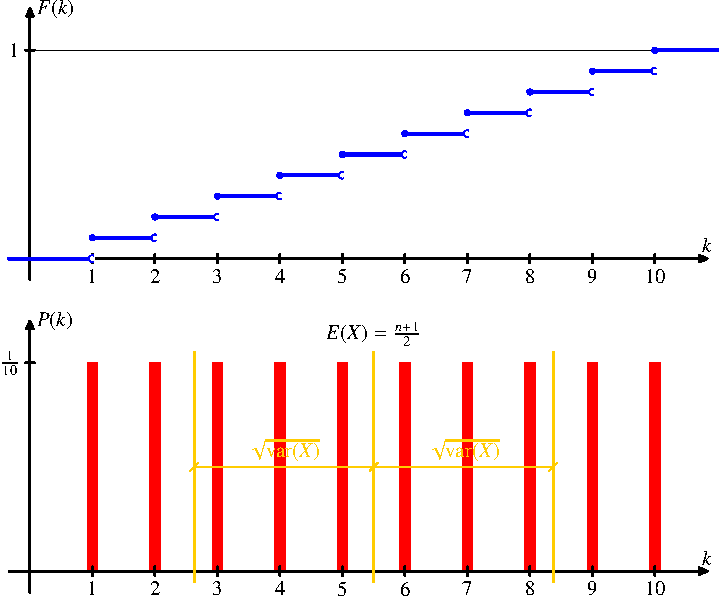
\includegraphics{images/gl-2.pdf}
\caption{Wahrscheinlichkeit und Verteilungsfunktion der diskreten Gleichverteilung
f"ur $n=10$
\label{graph-diskrete-gleichverteilung}}
\end{figure}

Bereits in Abschnitt \ref{section-laplace-ereignisse}
wurden Ereignisse
untersucht, bei denen alle Elementarereignisse mit gleicher Wahrscheinlichkeit
eingetreten sind.
Im Kontext einer Zufallsvariable bedeutet
Gleichverteilung, dass jeder m"ogliche Wert mit gleicher Wahrscheinlichkeit
vorkommt.
Im einfachsten Fall sind die Werte nat"urliche Zahlen
$\{1,\dots,n\}$, die Wahrscheinlichkeit f"ur den Wert ist 
$p(k)=\frac1n$.
Die Verteilungsfunktion dieser Verteilung ist
\[
F(x)=
\begin{cases}
0&\qquad x \le 1\\
{\displaystyle \frac{\left\lfloor x\right\rfloor}n}&\qquad 1\le x\le n\\
1&\qquad x \ge n
\end{cases}
\]
Entsprechend einfach sind Erwartungswert und Varianz zu berechnen:
{\allowdisplaybreaks
\begin{align*}
E(X)&=\sum_{k=1}^nkp(k)=\frac1n\sum_{k=1}^nk=\frac1n\cdot\frac{n(n+1)}{2}=\frac{n+1}2\\
E(X^2)&=\sum_{k=1}^nk^2p(k)=\frac1n\sum_{k=1}^nk^2=\frac1n\cdot\frac{n(1+3n+2n^2)}{6}=\frac{2n^2+3n+1}{6}\\
\operatorname{var}(X)&=E(X^2)-E(X)^2=\frac{2n^2+3n+1}{6}-\frac{(n+1)^2}4\\
&=\frac{4n^2+6n+2-3n^2-6n-3}{12}=\frac{n^2-1}{12}
\end{align*}
}
Die Wahrscheinlichkeit und die Verteilungsfunktion ist in
Abbildung~\ref{graph-diskrete-gleichverteilung} dargestellt.

%
% binomialverteilung.tex -- Abschnitt über Binomialverteilung im Kapitel 5
%
% (c) 2015 Prof Dr Andreas Mueller, Hochschule Rapperswil
%
\subsection{Binomialverteilung} \label{section-binomialverteilung}
\index{Bernoulli-Experiment}
\begin{table}
\renewcommand{\arraystretch}{1.5}
\begin{center}
\begin{tabular}{|l|l|}
\hline
Name&Binomialverteilung\\
\hline
Wahrscheinlichkeit&
\begin{minipage}{3.7in}
\vskip3pt
$\displaystyle P(k)=\binom{n}{k}p^k(1-p)^{n-k}$
\end{minipage}
\\[10pt]
Verteilungsfunktion&
$\displaystyle F(k)=\sum_{i=0}^k\binom{n}{i}p^i(1-p)^{n-i}$
\\[10pt]
Erwartungswert&$\displaystyle np$\\
Varianz&$\displaystyle np(1-p)$\\
\hline
Anwendungen&\begin{minipage}{3.7in}%
\strut
$\bullet$ Anzahl Eintreten eines Bernoulli-Experimentes
\strut
\end{minipage}\\
\hline
\end{tabular}
\end{center}
\caption{Datenblatt der Binomialverteilung\label{datenblatt:binomialverteilung}}
\end{table}
\begin{figure}
\centering
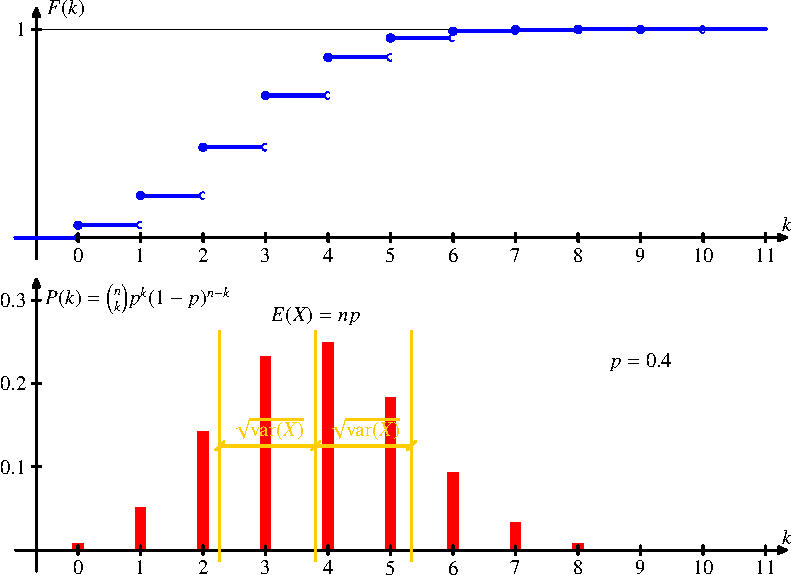
\includegraphics{images/gl-3.pdf}
\caption{Wahrscheinlichkeitsverteilung und Verteilungsfunktion einer
Binomialverteilung mit $p=0.4$ und $n=10$.
\label{binomialgraph}}
\end{figure}

Der Wurf einer M"unze ist der Spezialfall eines Versuches mit
zwei m"oglichen Ausg"angen $\{0,1\}$, bei dem die beiden Ausg"ange als
gleich wahrscheinlich angesehen werden. Es sind durchaus auch
Anwendungsf"alle denkbar, in denen die beiden Ausg"ange unterschiedliche
Wahrscheinlichkeit haben, zum Beispiel $p$ f"ur den Ausgang $1$ und $1-p$
f"ur $0$.
Ein solches Experiment nennt man ein Bernoulliexperiment.

Wir wiederholen jetzt dieses Experiment $n$ mal und betrachten die Ereignisse,
dass in genau $k$ der $n$ F"alle der Ausgang $1$ eingetreten ist,
und $0$ in allen anderen F"allen. Es gibt $\binom{n}{k}$ M"oglichkeiten,
die $k$ $1$-Experimente auszuw"ahlen, und die Kombination, dass genau
dieses Kombination $1$ und $0$ realisiert wird, ist $p^k(1-p)^{n-k}$.
Somit ist die Wahrscheinlichkeit, dass von $n$ Experimenten deren $k$
erfolgreich sind
\[
\binom{n}{k}p^k(1-p)^{n-k}.
\]
Dies ist die Binomialverteilung:
\index{Binomialverteilung}
\begin{definition}
Eine Zufallsvariable mit diskreten Werten $k\in\{0,\dots,n\}$
heisst binomialverteilt zum Parameter $p$, wenn die Wahrscheinlichkeit
des Wertes $k$ 
\[
\binom{n}{k}p^k(1-p)^{n-k}
\]
ist.
\end{definition}

Die Wahrscheinlichkeitsverteilung und die Verteilungsfunktion der
Binomialverteilung ist in Abbildung~\ref{binomialgraph} dargstellt.

\subsubsection{Erwartungswert und Varianz}
\index{Erwartungswert!der Binomialverteilung}
\index{Binomialverteilung!Erwartungswert}
Aus der bekannten Wahrscheinlichkeitsverteilung l"asst sich
Erwartungswert und Varianz berechnen:
\begin{satz}
Eine auf $\{0,\dots,n\}$ zum Parameter $p$ binomialverteilte Zufallsvariable
$X$ hat Erwartungswert
\[
E(X)=pn
\]
und Varianz
\[
\operatorname{var}(X)=np(1-p).
\]
Die maximale Varianz wird erreicht bei $p=\frac12$.
\end{satz}
\index{Varianz!der Binomialverteilung}
\index{Binomialverteilung!Varianz}

\begin{proof}[Beweis] Wir m"ussen die Summen
\begin{eqnarray*}
E(X)&=&\sum_{k=0}^nk\binom{n}{k}p^k(1-p)^{n-k}\\
E(X^2)&=&\sum_{k=0}^nk^2\binom{n}{k}p^k(1-p)^{n-k}
\end{eqnarray*}
berechnen k"onnen. Dazu betrachten wir die Hilfsfunktion
\[
f(x)=(x+y)^n=\sum_{k=0}^n\binom{n}{k}x^ky^{n-k},
\]
offensichtlich erhalten wir die Summe der Wahrscheinlichkeiten aller
binomailverteilten Werte, wenn
wir $x=p$ und $y=(1-p)$ einsetzen.
Die Ableitung nach $x$ gefolgt von Multiplikation mit $x$ liefert
\[
 x\frac{d}{dx}f(x)
=xn(x+y)^{n-1}\\
=\sum_{k=0}^n\binom{n}{k}kx^ky^{n-k}
\]
Nach Einsetzen von $x=p$ und $y=1-p$ entsteht rechts genau
der gesuchte Erwartungswert, links aber
\[
pn(p+1-p)^{n-1}=pn=\sum_{k=0}^n\binom{n}{k}kp^k(1-p)^{n-k}=E(X).
\]
Erneute Anwendung von $x\frac{d}{dx}$ liefert
\[
xn(x+y)^{n-1}+x^2 n(n-1)x^{n-2}=\sum_{k=0}^n\binom{n}{k}k^2x^ky^{n-k},
\]
und nach Einsetzen der Werte f"ur $x$ und $y$
\[
pn+p^2n(n-1)=\sum_{k=0}^n\binom{n}{k}k^2p^k(1-p)^{n-k}=E(X^2).
\]
Daraus bestimmen wir die Varianz
\[
\operatorname{var}(X)=E(X^2)-E(X)^2=pn+p^2n(n-1)-p^2n^2=p(1-p)n
\]
Die Funktion $p\mapsto np(1-p)$ ist eine quadratische Funktion mit den
Nullstellen $0$ und $1$. Quadratische Funktionen sind symmetrisch um
die Abszisse des Scheitelpunktes, der demzufolge in der Mitte zwischen
den Nullstellen bei $\frac12$ sein muss.
\end{proof}

\subsubsection{Der Grenzwert \texorpdfstring{$n\to\infty$}{n gegen unendlich}}
\index{Binomialverteilung!Normalapproximation}
Was geschieht, wenn die Zahl $n$ der Versuche beliebig vergr"ossert wird?
nat"urlich wird die Zahl der m"oglichen Werte der Zufallsvariable
gr"osser, der Erwartungswert $np$ und die Varianz $np(1-p)$ steigen.
Standardisiert man die Verteilung jedoch, indem man die Zufallsvariable
durch $Y=(X-np)/\sqrt{np(1-p)}$ ersetzt, dann wird die Zufallsvariable $Y$
Erwartungswert $0$ und Varianz $1$ haben. 

Durch die Skalierung r"ucken die m"oglichen Werte von $Y$ n"aher zusammen,
so dass man die Wahrscheinlichkeiten nicht direkt vergleichen kann.
Man kann aber die Verteilungsfunktionen $F_Y$ f"ur verschiedene Werte
von $n$ vergleichen. Aus dem zentralen Grenzwertsatz erh"alt man
jedoch die Aussage, dass die Verteilungsfunktion gegen die
Verteilungsfunktion der Standardnormalverteilung konvergieren wird.
Dieser Spezialfall des zentralen Grenzwertsatzes heisst auch der
Satz von de Moivre und Laplace.

Die Gr"osse $Y=(X-np)/\sqrt{np(1-p)}$ sollte also normalverteilt sein
mit Erwartungswert $0$ und Varianz $1$, aber nat"urlich nur, wenn $p$
tats"achlich die Wahrscheinlichkeit des einen Ausgangs des
Bernoulliexperimentes ist. Daraus l"asst sich jetzt ein Test daf"ur
konstruieren, ob $p$ die Wahrscheinlichkeit des einen Ausgangs eines
Bernoulliexperimentes ist. Ist $p$ n"amlich nicht die richtige
Wahrscheinlichkeit, wird f"ur grosse $Y$ mit grosser Wahrscheinlichkeit
stark von $0$ abweichen, es muss also nur ein Kriterium gefunden werden,
welches angibt, dass die Abweichung zu gross ist, um immer noch daran
zu glauben, dass das $p$ richtig war.

Ein rationales Kriterium l"asst sich mit der $\chi^2$-Verteilung konstruieren.
$Y^2$ ist $\chi^2$-verteilt mit einem Freiheitsgrad.
Die Wahrscheinlichkeit, dass $Y^2$ gr"osser ist als $M$ ist
\[
P(Y^2>M)=\int_M^\infty f_{\frac12,\frac12}(t)\,dt.
\]
Wenn wir also $M$ bestimmen, so dass diese Wahrscheinlichkeit 
zum Beispiel 5\% ist, dann glauben wir nicht mehr, dass $p$ tats"achlich
die Wahrscheinlichkeit des einen Ausgangs ist, sobald $Y^2>M$ wird,
und nur in 5\% aller F"alle werden wir dies zu unrecht tun.

%
% hypergeometrisch.tex -- Abschnitt über die hypergeometrische Verteilung in Kap 5
%
% (c) 2015 Prof Dr Andreas Mueller, Hochschule Rapperswil
%
\subsection{Hypergeometrische Verteilung} \label{section-hypergeometrischeverteilung}
\index{hypergeometrische Verteilung}
\index{hypergeometrische Verteilung!Erwartungswert}
\index{hypergeometrische Verteilung!Varianz}
\index{Varianz!hypergeometrische Verteilung}
\index{Erwartungswert!hypergeometrische Verteilung}
\begin{table}
\renewcommand{\arraystretch}{1.5}
\begin{center}
\begin{tabular}{|l|l|}
\hline
Name&Hypergeometrische Verteilung\\
\hline
Wahrscheinlichkeit&
\begin{minipage}{3.7in}
\vskip3pt
$\displaystyle
h(k|N;m;n)=
\left.\binom{M}{k}\binom{N-M}{n-k}\right/\binom{N}{n}
$
\end{minipage}
\\[10pt]
Erwartungswert&$\displaystyle n\frac{M}{N}$\\[10pt]
Varianz&$\displaystyle
n\frac{M(N-M)(N-n)}{N^2(N-1)}
$\\[10pt]
\hline
Anwendungen&\begin{minipage}{3.7in}%
\vskip3pt
\strut
$\bullet$ Lotto\\
$\bullet$ Auswahl von $n$ Elementen aus $N$ so dass $k$ von $M$ markierten
Elementen gew"ahlt werden
\strut
\end{minipage}\\[18pt]
\hline
\end{tabular}
\end{center}
\caption{Datenblatt der hypergeometrischen Verteilung\label{datenblatt:hypergeometrischeverteilung}}
\end{table}

Die hypergeometrische Verteilung wurde bereits in
(\ref{hypergeometrische-verteilung}) angetroffen.
$h(k|N;M;n)$ ist die
Wahrscheinlichkeit dass in einer $n$ Elemente umfassenden Stichprobe aus
einer Grundgesamtheit von $N$ Elementen, von denen $M$ eine spezielle
Eigenschaft besitzen, $k$ Elemente mit der Eigenschaft zu finden sind.
Es ist
\[
h(k|N;M;n)=\frac{\binom{M}{k}\binom{N-M}{n-k}}{\binom{N}{n}}.
\]
Da $h$ eine Verteilung ist, ist die Summe aller Wahrscheinlichkeiten
f"ur alle in Frage kommenden $k$
\[
\sum_{k=0}^nh(k|N;M;n)=1.
\]
\subsubsection{Erwartungswert und Varianz}
Der Erwartungswert ist
\begin{align*}
E(X)
&=\sum_{k=0}^n k\cdot\frac{\binom{M}{k}\binom{N-M}{n-k}}{\binom{N}{n}}\\
&=\sum_{k=1}^n \frac{M\binom{M-1}{k-1}\binom{N-M}{n-k}}{\frac{N}{n}\binom{N-1}{n-1}}\\
&=n\frac{M}{N}\sum_{k=0}^{n-1} \frac{\binom{M-1}{k}\binom{N-1-(M-1)}{n-1-k}}{\binom{N-1}{n-1}}\\
&=n\frac{M}{N}\sum_{k=0}^{n-1}h(k|N-1;n-1;M-1)\\
&=n\frac{M}{N}
\end{align*}
Unter dem letzten Summenzeichen stehen die Wahrscheinlichkeiten f"ur alle
F"alle einer hypergeometrischen Verteilung in Stichproben, die um eins kleiner
sind, deren Summe ist nat"urlich 1.

Analog kann man bei der Berechnung der Varianz vorgehen:
\begin{align*}
E(X^2)
&=\sum_{k=0}^n k^2h(k|N;M;n)\\
&=n\frac{M}{N}\sum_{k=0}^{n-1} (k+1)\cdot h(k|N-1;M-1;n-1)\\
&=n\frac{M}{N}(n-1)\frac{M-1}{n-1}\biggl(\sum_{k=0}^{n-2} h(k|N-2;M-2;n-2)+1\biggr)\\
&=n\frac{M}{N}\biggl((n-1)\frac{M-1}{N-1}+1\biggr)\\
\operatorname{var}(X)
&=n\frac{M}{N}\biggl((n-1)\frac{M-1}{N-1}+1-n\frac{M}{N}\biggr)\\
&=n\frac{M(N-M)(N-n)}{N^2(N-1)}
\end{align*}
\begin{satz}
Eine hypergeometrisch mit den Parametern $M$, $N$ und $n$
verteilte Zufallsgr"osse $X$
hat Erwartungswert
\[
E(X)=n\frac{M}{N}
\]
und Varianz
\[
\operatorname{var}(X)=n\frac{M(N-M)(N-n)}{N^2(N-1)}
\]
\end{satz}

%
% poissonverteilung.tex -- Abschnitt über Poissonverteilung in Kapitel 5
%
% (c) 2015 Prof Dr Andreas Mueller, Hochschule Rapperswil
%
\subsection{Poissonverteilung\label{section-poissonverteilung}}
\begin{figure}
\centering
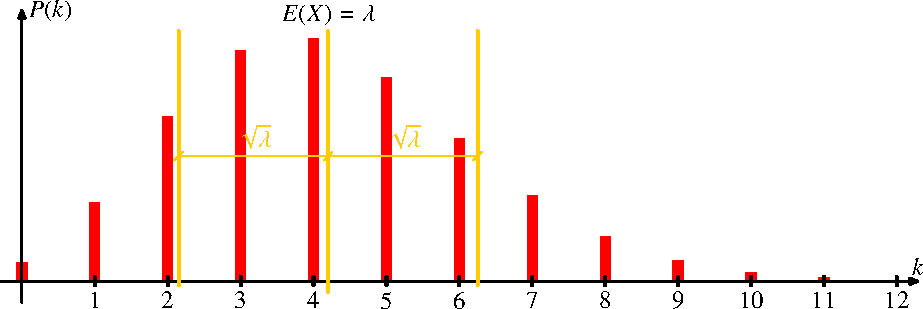
\includegraphics{images/exp-2.pdf}
\caption{Wahrscheinlichkeitsverteilung der Poisson-Verteilung f"ur
$\lambda=4.2$, $E(X)=\lambda$ und $\operatorname{var}(X)=\sqrt{\lambda}$.
\label{poisson-verteilung}}
\end{figure}
\begin{table}
\renewcommand{\arraystretch}{1.5}
\begin{center}
\begin{tabular}{|l|l|}
\hline
Name&Poissonverteilung\\
\hline
Wahrscheinlichkeit&
\begin{minipage}{3.7in}
\vskip3pt
$\displaystyle
P_\lambda(k)=\frac{\lambda^k}{k!}e^{-\lambda}
$
\end{minipage}
\\
Erwartungswert&$\displaystyle \lambda$\\
Varianz&$\displaystyle \lambda$\\
\hline
Anwendungen&\begin{minipage}{3.7in}%
\vskip3pt
\strut
$\bullet$ Anzahl Ereignisse mit exponentialverteilten Intervallen\\
$\bullet$ Approximation der Binomialverteilung f"ur seltene Ereignisse, die
mit Rate $\lambda$ eintreten
\strut
\end{minipage}\\[20pt]
\hline
\end{tabular}
\end{center}
\caption{Datenblatt der Poissonverteilung\label{datenblatt:poissonverteilung}}
\end{table}
Die Poissonverteilung liefert eine Antwort auf folgende Frage. In Abschnitt
\ref{section-exponentialverteilung} wurde die Exponentialverteilung
als die Verteilung f"ur die Ausfallwahrscheinlichkeit eines ``ged"achtnislosen''
Bauteils vorgestellt. Wir nehmen nun an, dass das Bauteil bei jedem Defekt
sofort ersetzt wird, und fragen danach, wie wahrscheinlich es ist, dass
wir in einem bestimmten Zeitintervall $k$ Ausf"alle beobachten.

Sei $X_i$ die Lebensdauer des Bauteils mit der Nummer $i$, es handelt
sich dabei um eine exponentialverteilte Zufallsvariable. Wenn im Zeitintervall
$[0,x]$ genau $k$ Ausf"alle beobachtet wurden, dann heisst das, dass die
Summe von $k$ Zufallsvariablen $\le x$ ist, jene von $k+1$ Zufallsvariable
aber $>x$. Also
\[
P(X_1+\dots+X_k\le x \wedge X_1+\dots+X_{k+1}>x)
\]
Wir berechnen diese Wahrscheinlichkeit in zwei Schritten.

Zun"achst interessiert uns, wie gross die Wahrscheinlichkeit ist, dass im
Intervall $[0,x]$ mindestens $k$ Ausf"alle passieren, dies ist
$P(X_1+\dots+X_k\le x)=F_{X_1+\dots+X_k}(x)$, also die Verteilungsfunktion
einer Summe von $k$ identisch exponentialverteilten Zufallsvariablen. Wir
behaupten:
\begin{satz}Sind $(X_i)_{1\le i\le k}$ identische exponentialverteilte,
unabh"angige Zufallsvariablen, dann hat deren Summe folgende Verteilungsfunktion
und Wahrscheinlichkeitsdichte:
\begin{align*}
F_{X_1+\dots+X_k}(x)&=\begin{cases}
{\displaystyle 1-e^{-ax}\sum_{i=0}^{k-1}\frac{(ax)^i}{i!}}&\qquad x \ge 0\\
0&\qquad x < 0
\end{cases}
\\
\varphi_{X_1+\dots+X_k}(x)&=\begin{cases}
{\displaystyle a^k\frac{x^{k-1}}{(k-1)!}e^{-ax}}&\qquad x\ge0\\
0&\qquad x < 0\end{cases}
\end{align*}
\end{satz}
\begin{proof}[Beweis]
Wir beweisen zun"achst die Formeln f"ur die Dichtefunktion $\varphi_k$ mit
Hilfe von vollst"andiger Induktion. F"ur $k=1$ liegt nur eine einzige
Zufallsvariable vor, durch Einsetzen von $k$ finden wir f"ur $x>0$
\[
\varphi_1(x)=ae^{-ax},
\]
also genau die Dichte der Exponentialverteilung. Offensichtlich ist dies
die richtige Wahrscheinlichkeitsdichte.

Wir nehmen nun an, dass obige Formel die Wahrscheinlichkeitsdichte f"ur die
Summe von $k$ Zufallsvariablen korrekt ist, und berechnen die daraus
folgende Wahrscheinlichkeitsdichte f"ur eine Summe von $k+1$ Zufallsvariablen.
Dazu wird die Faltung verwendet, es gilt f"ur $x>0$
\begin{align*}
\varphi_k*\varphi_1(x)
&=
\int_{-\infty}^{\infty}\varphi_k(t)\varphi_1(x-t)\,dt\\
&=\int_0^x a^k\frac{t^{k-1}}{(k-1)!}e^{-at}ae^{-a(x-t)}\,dt\\
&=a^{k+1}e^{-ax}\int_0^x \frac{t^{k-1}}{(k-1)!}\,dt\\
&=a^{k+1}e^{-ax}\left[\frac{t^k}{k!}\right]_0^x\\
&=a^{k+1}e^{-ax}\frac{x^k}{k!}=\varphi_{k+1}(x)
\end{align*}
Damit ist die Formel f"ur $\varphi_k$ f"ur alle $k$ gezeigt.

Aus der Wahrscheinlichkeitsdichte kann nun auch die Verteilungsfunktion
berechnet werden. Durch partielle Integration kann man die Verteilungsfunktion
wie folgt berechnen:
\begin{align*}
F_k(x)
&=\int_0^x\varphi_k(t)\,dt\\
&=\int_0^xa^k\frac{t^{k-1}}{(k-1)!}e^{-at}\,dt\\
&=\left[-a^{k-1}\frac{t^{k-1}}{(k-1)!}e^{-at}\right]_0^x+\int_0^xa^{k-1}\frac{t^{k-2}}{(k-2)!}e^-at\,dt\\
&=-a^{k-1}\frac{x^{k-1}}{(k-1)!}e^{-ax}+F_{k-1}(x)\\
&=-\frac{(ax)^{k-1}}{(k-1)!}e^{-ax}+F_{k-1}(x)
\end{align*}
Die Verteilungsfunktion $F_1$ von $\varphi_1$ kennen wir bereits:
\[
F_1(x)=\int_0^xae^{-at}\,dt=-e^{-ax}+1.
\]
Daraus leiten wir ab
\[
F_k(x)=1-e^{-ax}\sum_{i=0}^{k-1}\frac{(ax)^i}{i!}
\]
Die Summe ist die Partialsumme f"ur die Reihenentwicklung von $e^{ax}$,
insbesondere ist die Partialsumme immer kleiner als $a^{ax}$, also
\[
e^{-ax}\sum_{i=0}^{k-1}\frac{(ax)^i}{i!}<e^{-ax}\cdot e^{ax}=1,
\]
und damit $F_k(x) \le 0$. Andererseits ist die Partialsumme nur ein
Polynom in $x$, welches niemals so schnell wachsen kann wie $e^{-ax}$ kleiner
wird. Im Grenzwert $x\to\infty$ verschwindet der zweite Summand daher und
es gilt wie zu erwarten ist $\lim_{x\to\infty}F_k(x)=1$.
\end{proof}
Die hier gefundenen Verteilungen sind auch von einiger praktischer Bedeutung,
sie heissen die Erlang-Verteilungen.
\index{Erlang-Verteilung}

Um nun die Wahrscheinlichkeit $P_k(x)$ des Auftretens von genau $k$ Ausf"allen
ist jetzt also die Wahrscheinlichkeit, dass bis zur Zeit $x$ mindestens
$k$ Ausf"allen aufgetreten sind minus die Wahrscheinlichkeit, dass mehr
als $k$ Ausf"alle aufgetreten sind: 
\[
P_k(x)=P(\text{mindestens $k$ Ausf"alle})-P(\text{mehr als $k$ Ausf"alle})
\]
Die Wahrscheinlichkeit von mehr als $k$ Ausf"allen ist aber die Wahrscheinlichkeit
von mindestens $k+1$ Ausf"allen, also
\begin{align*}
P_k(x)
&=P(\text{mindestens $k$ Ausf"alle})-P(\text{mindestens $k+1$ Ausf"alle})\\
&=F_k(x)-F_{k+1}(x)\\
&=1-e^{-ax}\sum_{i=0}^{k-1}\frac{(ax)^i}{i!}-1+e^{-ax}\sum_{i=0}^{k}\frac{(ax)^i}{i!}\\
&=e^{-ax}\frac{(ax)^k}{k!}
\end{align*}
Somit haben wir die Wahrscheinlichkeit berechnet, dass im betrachteten
Intervall genau $k$ Bauteile versagen.
Dies f"uhrt uns zur Definition der Poissonverteilung:
\begin{definition} Die Poissonverteilung
\[
P_\lambda(k)=\frac{\lambda^k}{k!}e^{-\lambda}
\]
beschreibt f"ur $\lambda=ax$ die Wahrscheinlichkeit,
dass in einem Zeitintervall $[0,x]$ genau $k$ Ereignisse eintreten, wenn
die Zeit zwischen den Ereignissen exponentialverteilt ist mit Dichte
$ae^{-ax}$.
\end{definition}

\subsubsection{Erwartungswert und Varianz}
\index{Poissonverteilung!Erwartungswert}
\index{Poissonverteilung!Varianz}
\index{Erwartungswert!Poissonverteilung}
\index{Varianz!Poissonverteilung}
Mit Hilfe der geschlossenen Formel f"ur die Poissonverteilung kann man
jetzt auch Erwartungswert und Varianz berechnen:
\begin{align*}
E(X)
&=\sum_{k=0}^\infty kP_\lambda(k)\\
&=\sum_{k=0}^\infty k\frac{\lambda^k}{k!}e^{-\lambda}\\
&=\lambda e^{-\lambda}\sum_{k=1}^\infty\frac{\lambda^{k-1}}{(k-1)!}\\
&=\lambda e^{-\lambda}\sum_{k=0}^\infty\frac{\lambda^k}{k!}\\
&=\lambda e^{-\lambda}e^\lambda=\lambda\\
\end{align*}
F"ur $E(X^2)$ finden wir analog
\begin{align*}
E(X^2)
&=\sum_{k=0}^\infty k^2P_\lambda(k)\\
&=\sum_{k=0}^\infty k^2\frac{\lambda^k}{k!}e^{-\lambda}\\
&=\lambda e^{-\lambda}\sum_{k=1}^\infty k\frac{\lambda^{k-1}}{(k-1)!}\\
&=\lambda e^{-\lambda}\frac{d}{d\lambda}\sum_{k=1}^\infty \frac{\lambda^k}{(k-1)!}\\
&=\lambda e^{-\lambda}\frac{d}{d\lambda}\lambda\sum_{k=1}^\infty \frac{\lambda^{k-1}}{(k-1)!}\\
&=\lambda e^{-\lambda}\frac{d}{d\lambda}\lambda e^{\lambda}\\
&=\lambda e^{-\lambda}(e^\lambda+\lambda e^\lambda)\\
&=\lambda(1+\lambda)
\end{align*}
Daraus erhalten wir die Varianz:
\[
\operatorname{var}(X)=E(X^2)-E(X)^2=\lambda^2+\lambda -\lambda^2 =\lambda.
\]
\begin{satz}
Die Poissonverteilung $P\lambda(k)$ hat Erwartungswert
$E(X)=\lambda$ und Varianz $\operatorname{var}(X)=\lambda$.
\end{satz}

\subsubsection{Poissonverteilung als Approximation f"ur die Binomialverteilung}
\index{Poissonverteilung!Approximation der Binomialverteilung}
Das folgende Experiment soll diese Anwendung motivieren: 18 mal werden zwei 
W"urfel geworfen, und in einem $6\times 6$-Feld das Feld mit der
erw"urfelten Zeilen- und Spalten-Nummer angekreuzt. Dabei muss man darauf
achten, immer den gleichen W"urfel f"ur die Zeilen-Nummern zu verwenden.
Dann wird ausgez"ahlt, wieviele Felder $k=0$, $k=1$, $k=2$,\dots\ Kreuze
enthalten.

Nat"urlich ist dies ein Bernoulli-Experiment. Die Wahrscheinlichkeit, ein
bestimmtes Feld anzukreuzen, ist $p=\frac{1}{36}$, das Experiment
wird $18$ mal wiederholt. Die Wahrscheinlichkeit $P(k)$, dass das Feld $k$ mal
angekreuzt wurde, ist durch die Binomialverteilung gegeben:
\[
P(k)=\binom{n}{k}p^k(1-p)^{n-k}.
\]

Leider ist dieser Ausdruck f"ur grosses $n$ schwierig auszurechnen.
Wir suchen also nach einer Approximation, die leichter auszuwerten ist.
Dabei k"onnen wir nicht einfach $n\to\infty$ gehen lassen, denn die
Wahrscheinlichkeit $P(k)$ w"urde dann auch anwachsen. Wir m"ussen
gleichzeitig die Wahrscheinlichkeit kleiner machen, so dass die Rate $\lambda$,
mit der Kreuze gemacht werden, gleich bleibt. Im Experiment wird
die H"alfte ($\lambda=\frac{18}{36}=\frac12$) der Felder angekreuzt.
Die Wahrscheinlichkeit $p$ muss also mit $\lambda$ "uber die Formel
\[
p=\frac{\lambda}{n}
\]
zusammenh"angen.

\begin{figure}
\begin{center}
\begin{tabular}{|r|r|r|r|r|}
\hline
$k$&Binomial&empirisch&Poisson&\\
\hline
0&   0.60440867 & 0.60226943 & 0.60653066 & 21.8351 \\
1&   0.30646073 & 0.30971007 & 0.30326533 & 10.9176 \\
2&   0.07553610 & 0.07521756 & 0.07581633 &  2.7294 \\
3&   0.01205740 & 0.01146811 & 0.01263606 &  0.4549 \\
4&   0.00140104 & 0.00123035 & 0.00157951 &  0.0569 \\
5&   0.00012629 & 0.00009816 & 0.00015795 &  0.0057 \\
6&   0.00000919 & 0.00000599 & 0.00001316 &  0.0005 \\
7&   0.00000055 & 0.00000031 & 0.00000094 &  0.0000 \\
8&   0.00000003 & 0.00000002 & 0.00000006 &  0.0000 \\
9&   0.00000000 & 0.00000000 & 0.00000000 &  0.0000 \\
\hline
\end{tabular}
\end{center}
\caption{Wahrscheinlichkeit, in einem $6\times 6$-Feld nach 18-maligem
zuf"alligem Ankreuzen eines Feldes gefunden Verteilung der Anzahl Kreuze.
Die Spalte ganz rechts enth"alt die erwartet Anzahl Felder mit $k$ Kreuzen.
\label{cross36}}
\end{figure}

Damit kann man jetzt die Approximation durchf"uhren:
\begin{align*}
\binom{n}{k}p^k(1-p)^{n-k}
&=
\frac{n(n-1)(n-2)\dots(n-k+1)}{k!}\cdot \biggl(\frac{\lambda}n\biggr)^k\cdot \biggl(1-\frac{\lambda}n\biggr)^{n-k}\\
&=
\frac{\lambda^k}{k!}
\cdot\frac{n}{n}
\cdot\frac{n-1}{n}
\cdot\frac{n-2}{n}
\dots
\cdot\frac{n-k+1}{n}
\cdot
\biggl(1-\frac{\lambda}n\biggr)^n
\cdot
\biggl(1-\frac{\lambda}n\biggr)^{-k}
\end{align*}
F"ur $n\to\infty$ strebt der letzte Term gegen $1$.
Der zweitletzte Term strebt gegen $e^{-\lambda}$.
Jeder der Faktoren $\frac{n-i}n$ strebt gegeben $1$, und es sind ja nur
$k$ solche Faktoren, $k$ bleibt w"ahrend des Grenz"ubergangs unver"andert.
Daraus leiten wir ab:
\[
\lim_{n\to\infty} 
\binom{n}{k}p^k(1-p)^{n-k}
=
\frac{\lambda^k}{k!}e^{-\lambda}=P_{\lambda}(k),
\]
die Poisson-Verteilung zum Parameter $\lambda$.

Wenden wir dies auf das urspr"ungliche Experiment an, also $n=36$,
$\lambda=0.5$, finden wir die Resultate in Tabelle~\ref{cross36}. 
Die Abweichungen in der Spalte der empirischen Resultate kommt "ubrigens
nicht daher, dass zu wenige Versuch gemacht worden w"aren, sondern daher,
dass wir jeweils immer alle Felder ausgez"ahlt haben. Diese sind aber nicht
unabh"angig. Die beim Ausz"ahlen des $6\times 6$-Feldes gefundenen Werte
sind also gar nicht die Resultate von $n$ unabh"angigen Bernoulli-Experimenten.



\input schaetzen.tex
\input testen.tex
\input filter.tex
\appendix
%\input junkscience.tex
\chapter{Verteilungs-Datenbl"atter\label{appendix-datenblaetter}}
Die folgenden Abschnitte stellen die wichtigsten Eigenschaften der
verschiedenen in fr"uheren Kapiteln behandelten Verteilungen zusammen.

\section{Gleichverteilung}
%
% db-gleichverteilung.tex -- Datenblatt der stetigen gleichverteilung
%
% (c) 2015 Prof Dr Andreas Mueller, Hochschule Rapperswil
%
\subsection{Steckbrief}
\begin{center}
\begin{tabular}{|l|l|}
\hline
Name&Gleichverteilung\\
\hline
Dichtefunktion&
\begin{minipage}{3.7in}
\vskip5pt
$\displaystyle
\begin{cases}
\frac1{b-a}&\qquad a\le x\le b\\
0&\qquad\text{sonst}
\end{cases}
$
\end{minipage}
\\[8pt]
Verteilungsfunktion&
\begin{minipage}{3.7in}
\vskip5pt
$\displaystyle
\begin{cases}0&\qquad x\le a\\
\frac{x-a}{b-a}&\qquad x \le a \le b\\
1&\qquad x>b\end{cases}
$
\end{minipage}
\\[8pt]
Erwartungswert&
\begin{minipage}{3.7in}
\vskip3pt
$\displaystyle \frac{a+b}2$
\end{minipage}
\\[8pt]
Varianz&
\begin{minipage}{3.7in}
\vskip3pt
$\displaystyle \frac{(b-a)^2}{12}$
\end{minipage}
\\[8pt]
Median&
\begin{minipage}{3.7in}
\vskip3pt
$\displaystyle \frac{a+b}{2}$
\end{minipage}
\\[8pt]
$P(|X-E(X)|>\varepsilon)$&
\begin{minipage}{3.7in}
\vskip3pt
$\displaystyle 1-\frac{2\varepsilon}{b-a}$ für $\varepsilon<\frac{b-a}2$
\end{minipage}
\\[10pt]
\hline
Anwendungen&\begin{minipage}{3.7in}%
\strut
$\bullet$ Verteilung von Zufallszahlen
\strut
\end{minipage}\\
\hline
\end{tabular}
\end{center}

\subsection{Verteilungsfunktion und Wahrscheinlichkeitsdichte}
Verteilungsfunktion (oben) und Wahrscheinlichkeitsdichte (unten)
der Gleichverteilung:
\begin{center}
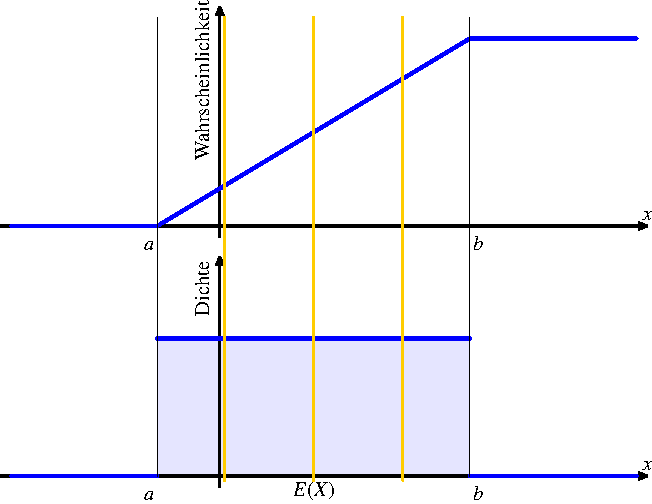
\includegraphics[width=0.8\hsize]{images/verteilungsfunktion-7}
\end{center}

\subsection{Wahrscheinlichkeit einer grossen Abweichung}
Wahrscheinlichkeit einer Abweichung vom Mittelwert einer
in $[0,1]$ gleichverteilten Zufallsvariable (rot) im Vergleich mit
der oberen Schranke aus dem Satz von Tschebyscheff (grün):
\begin{center}
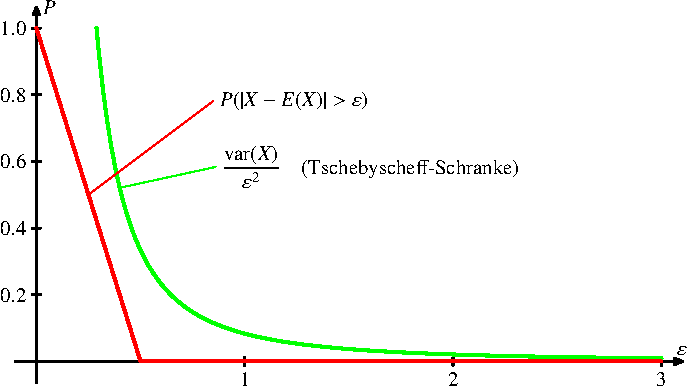
\includegraphics{images/gl-1.pdf}
\end{center}

\subsection{Parameter schätzen}
Die Parameter $a$ und $b$ der Gleichverteilung können mit den 
erwartungstreuen Schätzern
\begin{align*}
\hat a(x_1,\dots,x_n)=\frac{n+1}{n}\min(x_1,\dots,x_n)\\
\hat b(x_1,\dots,x_n)=\frac{n+1}{n}\max(x_1,\dots,x_n)
\end{align*}
geschätzt werden.

\vfill
\pagebreak

\section{Exponentialverteilung}
%
% db-exponentialverteilung.tex -- Datenblatt der Exponentialverteilung
%
% (c) 2015 Prof Dr Andreas Mueller, Hochschule Rapperswil
%
\subsection{Steckbrief}
\begin{center}
\renewcommand{\arraystretch}{2}
\begin{tabular}{|l|l|}
\hline
Name&Exponentialverteilung\\
\hline
Dichtefunktion&$\displaystyle ae^{-ax}$\\
Verteilungsfunktion&$1-e^{-ax}$\\
Erwartungswert&$\displaystyle \frac1a$\\
Varianz&$\displaystyle \frac1{a^2}$\\
Median&$\displaystyle \frac1a\log 2$\\[8pt]
$P(|X-E(X)|>\varepsilon)$&
\begin{minipage}{3.7in}
$
\begin{cases}
e^{-a\varepsilon-1}&\qquad\text{f"ur $\varepsilon > \frac1a$}\\
1-e^{a\varepsilon-1}+e^{-a\varepsilon-1}&\qquad\text{f"ur $\varepsilon \le \frac1a$}
\end{cases}
$
\end{minipage}
\\[10pt]
\hline
Anwendungen&\begin{minipage}{3.7in}%
\strut
$\bullet$ Prozess ohne Erinnerungsverm"ogen\\
$\bullet$ Radioaktivit"at
\strut
\end{minipage}\\
\hline
\end{tabular}
\end{center}

\subsection{Verteilungsfunktion und Wahrscheinlichkeitsdichte}
Verteilungsfunktion (oben) und Dichtefunktion (unten) der
Exponentialverteilung:
\begin{center}
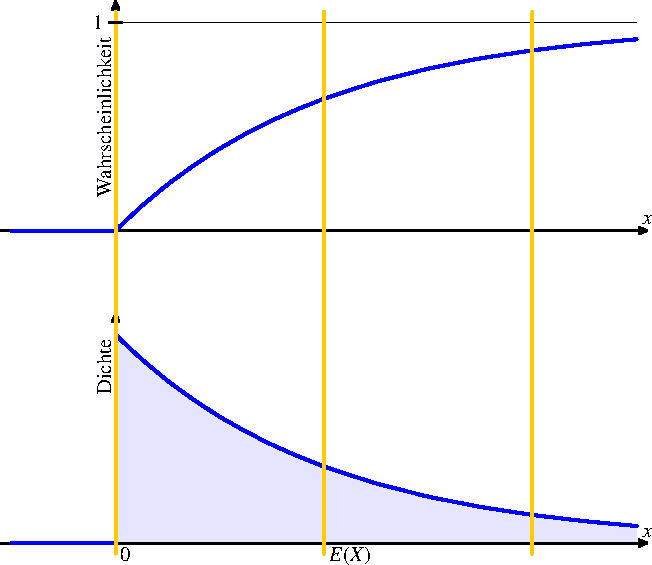
\includegraphics[width=0.8\hsize]{images/verteilungsfunktion-8}
\end{center}

\subsection{Wahrscheinlichkeit grosser Abweichungen}
Wahrscheinlichkeit f"ur eine grosse Abweichung bei einer
Exponentialverteilten Zufallsvariable, oben die durch den Satz von Tschebyscheff
gegebene Schranke (gr"un), unten die exakte Rechnung mit
Hilfe der Exponentialvereteilung (rot):
\begin{center}
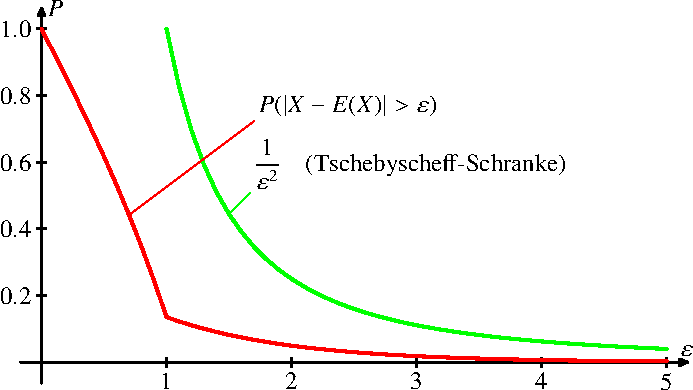
\includegraphics{images/exp-1.pdf}
\end{center}

\subsection{Parameter sch"atzen}
Der Parameter $1/a$ kann mit dem erwartungstreuen Sch"atzer
\[
\frac1{\hat a(x_1,\dots,x_n)}=\frac{x_1+\dots+x_n}n
\]
gesch"atzt werden.

\subsection{Erlang-Verteilungen}
Sie $X_i$ unabh"angige, identisch mit Parameter $a$ exponentialverteilte
Zufallsvariablen.
Dann ist $X_1+\dots+X_n$ Erlang-verteilt. 
Die Erlang-Verteilungen wurden f"ur die Analyse von Telefonzentralen erfunden,
und sind allgemein in der Queueing-Theorie n"utzlich.
Die Wahrscheinlichkeitsdichte und die Verteilungsfunktionen sind
\begin{align*}
F_{X_1+\dots+X_k}(x)&=\begin{cases}
\displaystyle 1-e^{-ax}\sum_{i=0}^{k-1}\frac{(ax)^i}{i!}&\qquad x\ge 0\\
\displaystyle 0&\qquad x < 0
\end{cases}
\\
\varphi_{X_1+\dots+X_k}(x)&=\begin{cases}
\displaystyle a^k\frac{x^{k-1}}{(k-1)!}e^{-ax}&\qquad x\ge 0\\
\displaystyle 0&\qquad x<0.
\end{cases}
\end{align*}

\vfill
\pagebreak

\section{Normalverteilung}
%
% db-normalverteilung.tex -- datenblatt der Normalverteilung
%
% (c) 2015 Prof Dr Andreas Mueller, Hochschule Rapperswil
%
\subsection{Steckbrief}
\begin{center}
\renewcommand{\arraystretch}{2}
\begin{tabular}{|l|l|}
\hline
Name&Normalverteilung\\
\hline
\setlength{\extrarowheight}{2pt}
Dichtefunktion&$\displaystyle\frac{1}{\sqrt{2\pi}\sigma}e^{-\frac{(x-\mu)^2}{2\sigma^2}}$\\
Verteilungsfunktion&keine elementare Funktion\\
Erwartungswert&$\mu$\\
Varianz&$\sigma^2$\\
Median&$\mu$\\
$P(|X-E(X)|>\varepsilon)$&keine einfache Formel\\
\hline
%\setlength{\extrarowheight}{50pt}
Anwendungen&
\begin{minipage}{3.7in}%
\vskip4pt
\strut
$\bullet$ Messwerte\\
$\bullet$ Summe vieler kleiner Einflüsse vergleichbar grosser Varianz
(Zentraler Grenzwertsatz)
\\
$\bullet$ Approximation der Binomialverteilung
\strut
\end{minipage}\\[21pt]
\hline
\end{tabular}
\end{center}

\subsection{Verteilungsfunktion und Wahrscheinlichkeitsdichte}
Verteilungsfunktion (oben) und Dichtefunktion (unten) der Normalverteilung:
\begin{center}
%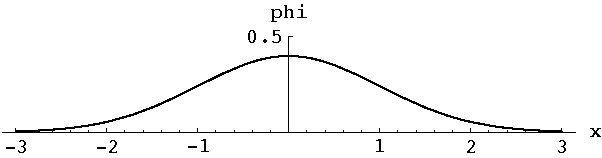
\includegraphics[width=0.8\hsize]{graphics/normphi}
%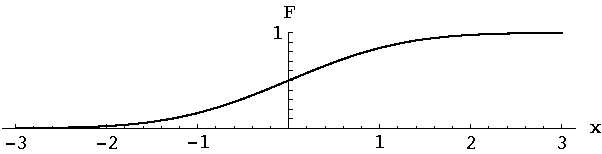
\includegraphics[width=0.8\hsize]{graphics/normF}
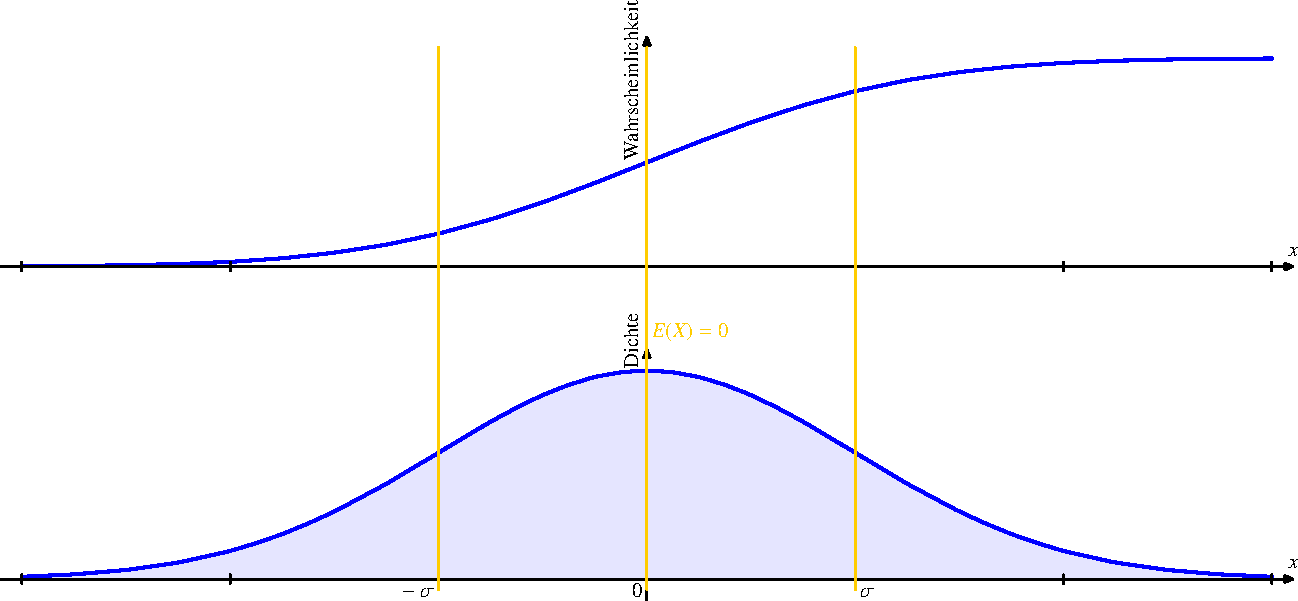
\includegraphics[width=\hsize]{images/verteilungsfunktion-9}
\end{center}

\subsection{Wahrscheinlichkeit einer grossen Abweichung}
Vergleich der Wahrscheinlichkeit für eine grosse Abweichung
für die Normalverteilung (rot) und die Schranke von Tschebyscheff (grün):
\begin{center}
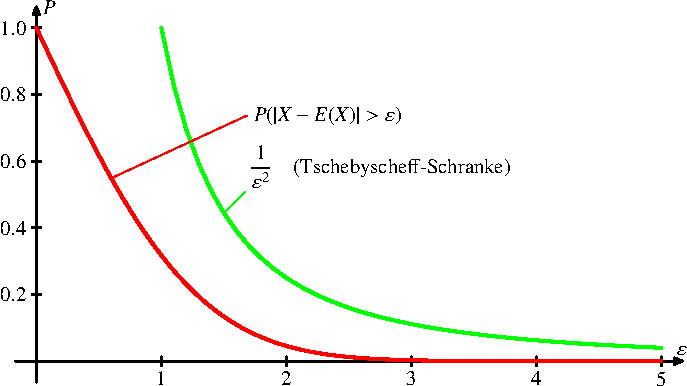
\includegraphics{images/norm-1.pdf}
\end{center}

\subsection{Parameter schätzen}
Die Parameter $\mu$ und $\sigma$ können mit den erwartungstreuen Schätzern
\begin{align*}
\hat\mu(x_1,\dots,x_n)&=\frac{x_1+\dots+x_n}{n}\\
\hat\sigma(x_1,\dots,x_n)^2&=\frac{1}{n-1}\biggl(
\sum_{i=1}^n x_i^2 - \frac1n\biggl(\sum_{i=1}^n x_i\biggr)^2
\biggr)
\end{align*}
geschätzt werden.

Der Mittelwert ist $\hat\mu(x_1,\dots,x_n)$ ist normalverteilt mit Erwartungswert
$\mu$ und Varianz $\frac1n\sigma^2$.
Die Stichprobenvarianz $\hat\sigma(x_1,\dots,x_n)^2/\sigma^2$ ist $\chi^2$-verteilt
mit $n-1$ Freiheitsgraden.

\subsection{Zentraler Grenzwertsatz}
Der zentrale Grenzwertsatz besagt, dass die Verteilungsfunktion einer Summe
einer grossen Zahl von Zufallsvariablen unter milden Voraussetzungen
gegen die Verteilungsfunktion einer Normalverteilung konvergiert.
Dies rechtfertigt den Einsatz der Normalverteilung als Modell für Prozesse,
in denen eine grosse Zahl von vergleichbar grossen Einflüssen zu einem Effekt
beitragen, zum Beispiel bei Messwerten.

\subsection{Standardisierung}
Ist $X$ eine normalverteilte Zufallsvariable, dann ist 
\[
Z=\frac{X-\mu}{\sigma}
\]
eine normalverteilte Zufallsvariable mit Erwartungswert $0$ und Varianz $1$,
d.~h.~eine standardnormalverteilte Zufallsvariable.
Für die Standardnormalverteilung ist im Tabellenanhang eine Tabelle der
Verteilungsfunktion sowie einzelner Quantilen zu finden.

Man beachte, dass die Zufallsvariable $Z$ nicht mehr normalverteilt ist, wenn man
$\mu$ und $\sigma$ durch Schätzwerte ersetzt, die resultierende Verteilung
ist dann eine $t$-Verteilung.

\vfill
\pagebreak

\section{Potenzgesetz, Pareto-Verteilung}
%
% db-paretoverteilung.tex -- Datenblatt der Pareto-Verteilung
%
% (c) 2015 Prof Dr Andreas Mueller, Hochschule Rapperswil
%
\subsection{Steckbrief}
\begin{center}
\renewcommand{\arraystretch}{2}
\begin{tabular}{|l|l|}
\hline
Name&Potenzverteilung, Pareto-Verteilung\\
\hline
Dichtefunktion&
\begin{minipage}{3.7in}
\vskip5pt
$\displaystyle
\begin{cases}
\frac{\alpha-1}{x_{\min}}\biggl(\frac{x}{x_{\text{min}}}\biggr)^{-\alpha}&\qquad x>x_{\text{min}}\\
0&\qquad\text{sonst}
\end{cases}
$
\end{minipage}
\\[15pt]
Verteilungsfunktion&
\begin{minipage}{3.7in}
\vskip3pt
$\displaystyle
\begin{cases}
1-\biggl(\frac{x}{x_{\text{min}}}\biggr)^{1-\alpha}&\qquad x>x_{\text{min}}\\
0&\qquad\text{sonst}
\end{cases} $
\end{minipage}
\\
Erwartungswert&$\displaystyle\frac{\alpha-1}{\alpha-2}x_{\text{min}}$,
undefiniert f"ur $\alpha\le 2$\\
Varianz&$\displaystyle
\biggl(
\frac{\alpha-1}{\alpha -3}-\biggl(\frac{\alpha-1}{\alpha-2}\biggr)^2
\biggr)x_{\text{min}}^2$, undefiniert f"ur $\alpha \le 3$\\
$P(|X-E(X)|>\varepsilon)$&$\displaystyle $ \\
Median&$2^{\frac1{\alpha-1}}x_{\text{min}}$\\
\hline
Anwendungen&\begin{minipage}{3.7in}%
\vskip5pt
\strut
$\bullet$ H"aufkeitsverteilung f"ur skaleninvariante Prozesse\\
$\bullet$ Einkommensverteilung\\
$\bullet$ Gr"osse und H"aufigkeit von Mondkratern\\
$\bullet$ Verkaufszahlen von B"uchern\\
$\bullet$ Einwohnerzahlen von St"adten
\strut
\end{minipage}\\[28pt]
\hline
\end{tabular}
\end{center}

\subsection{Wahrscheinlichkeitsdichte}
Wahrscheinlichkeitsdichte einer Potenzverteilung mit $\alpha=2.5$,
diese Verteilung hat keine Varianz:
\begin{center}
\includegraphics{images/power-2.pdf}
\end{center}

Wahrscheinlichkeitsdichte einer Potenzverteilung mit $\alpha=3.5$:
\begin{center}
\includegraphics{images/power-3.pdf}
\end{center}

\subsection{80/20-Regeln}
Potenzgesetze geben Anlass zu 80/20-Regeln.
Wir bezeichnen die Wahrscheinlichkeit des Auftretens von Werten $x>0$ 
mit $P(x)=1-F(x)$ und den Anteil des Erwartungswertes dieser Wert
am gesamten Erwartungswert  mit
\[
W(x)=\frac{\int_x^\infty \xi\varphi(\xi)\,d\xi}{\int_{x_{\text{min}}}^\infty \xi\varphi(\xi)\,d\xi}.
\]
Man kann $W(x)$ als den Anteil des ``Wertes'' interpretieren,
den die Werte oberhalb von $x$ beisteuern.
Es ist klar, dass $P(x)=1$ auch bedeutet, $W(x)=1$: 100\% der Werte
tragen 100\% des Wertes bei.
Die Definitionen besagen, dass f"ur beliebiges $x$ der obere $P(x)$-Anteil
der Werte den Anteil $W(x)$ des gesamten Wertes beitragen.
Es gilt
\[
W(x)= P(x)^{\frac{\alpha-2}{\alpha-1}}.
\]
Kurven $(P(x),W(x))$ f"ur verschiedene Werte von $\alpha$:
\begin{center}
\includegraphics{images/power-4.pdf}
\end{center}


\vfill
\pagebreak

\section{Binomialverteilung}
%
% db-binomialverteilung.tex -- Datenblatt der Binomialverteilung
%
% (c) 2015 Prof Dr Andreas Mueller, Hochschule Rapperswil
%
\subsection{Steckbrief}
\begin{center}
\renewcommand{\arraystretch}{1.5}
\begin{tabular}{|l|l|}
\hline
Name&Binomialverteilung\\
\hline
Wahrscheinlichkeit&
\begin{minipage}{3.7in}
\vskip3pt
$\displaystyle P(k)=\binom{n}{k}p^k(1-p)^{n-k}$
\end{minipage}
\\[10pt]
Verteilungsfunktion&
$\displaystyle F(k)=\sum_{i=0}^k\binom{n}{i}p^i(1-p)^{n-i}$
\\[10pt]
Erwartungswert&$\displaystyle np$\\
Varianz&$\displaystyle np(1-p)$\\
\hline
Anwendungen&\begin{minipage}{3.7in}%
\strut
$\bullet$ Anzahl Eintreten eines Bernoulli-Experimentes
\strut
\end{minipage}\\
\hline
\end{tabular}
\end{center}

\subsection{Verteilungsfunktion und Wahrscheinlichkeitsverteilung}
Wahrscheinlichkeitsverteilung und Verteilungsfunktion einer
Binomialverteilung mit $p=0.4$ und $n=10$:
\begin{center}
\includegraphics{images/gl-3.pdf}
\end{center}

\subsection{Parameter sch"atzen}
Wir ein Bernoulli-Experiment mit $m$ Wiederholungen $n$ mal wiederholt, erh"alt
man $n$ Werte $k_1,\dots,k_n$.
Die Wahrscheinlichkeit $p$ kann daraus mit Hilfe des Mittelwertes erwartungstreu
gesch"atzt werden:
\[
\hat p(k_1,\dots, k_n)=\frac{k_1+\dots+k_n}{n}.
\]
Als Sch"atzer f"ur den Parameter $m$ liegt das Maximum nahe, da aber
grosse Werte sehr selten sind, ist dieser Sch"atzer von unbrauchbarer
Qualit"at.


\vfill
\pagebreak

\section{Poisson-Verteilung}
%
% db-poissonverteilung.tex -- Datenblatt der Poisson-Verteilung
%
% (c) 2015 Prof Dr Andreas Mueller, Hochschule Rapperswil
%
\subsection{Steckbrief}
\begin{center}
\renewcommand{\arraystretch}{1.5}
\begin{tabular}{|l|l|}
\hline
Name&Poissonverteilung\\
\hline
Wahrscheinlichkeit&
\begin{minipage}{3.7in}
\vskip3pt
$\displaystyle
P_\lambda(k)=\frac{\lambda^k}{k!}e^{-\lambda}
$
\end{minipage}
\\
Erwartungswert&$\displaystyle \lambda$\\
Varianz&$\displaystyle \lambda$\\
\hline
Anwendungen&\begin{minipage}{3.7in}%
\vskip3pt
\strut
$\bullet$ Anzahl Ereignisse mit exponentialverteilten Intervallen\\
$\bullet$ Approximation der Binomialverteilung f"ur seltene Ereignisse, die
mit Rate $\lambda$ eintreten
\strut
\end{minipage}\\[20pt]
\hline
\end{tabular}
\end{center}

\subsection{Wahrscheinlichkeitsverteilung}
Wahrscheinlichkeitsverteilung der Poisson-Verteilung f"ur
$\lambda=4.2$, $E(X)=\lambda$ und $\operatorname{var}(X)=\sqrt{\lambda}$.
\begin{center}
\includegraphics{images/exp-2.pdf}
\end{center}

\subsection{Sch"atzung des Parameters $\lambda$}
Der Parameter $\lambda$ ist der Erwartungswert einer Poisson-Verteilung,
er l"asst sich daher mit dem Mittelwert
\[
\hat\lambda(k_1,\dots,k_n)=\frac{k_1+\dots+k_n}n
\]
erwartungstreu sch"atzen.


\vfill

%
% e03-tabellen.tex -- Tabellen wichtiger Verteilungen
%
% (c) 2006 Prof Dr Andreas Mueller, Hochschule Rapperswil
% $Id: e03-tabellen.tex,v 1.4 2008/09/09 14:22:16 afm Exp $
%
\rhead{Tabellen}
\chapter{Tabellen} \label{anhang-tabellen}

\begin{table}[ht]
\begin{center}
\begin{tabular}{|l|r|}
\hline
$p$&$x$\\
\hline
0.75&0.6745\\
0.8&0.8416\\
0.9&1.2816\\
0.95&1.6449\\
0.975&1.9600\\
0.99&2.3263\\
0.995&2.5758\\
0.999&3.0902\\
0.9995&3.2905\\
\hline
\end{tabular}
\end{center}
\caption{Quantilen der Normalverteilung\label{tabelle-normalquantilen}
\index{Tabelle!Normalverteilung!Quantilen}
}
\end{table}

\begin{table}[ht]
\begin{center}
%\scriptsize
\small
\begin{tabular}{|r|rrrrrrrrrr|}
\hline
$x$&+0.00&+0.01&+0.02&+0.03&+0.04&+0.05&+0.06&+0.07&+0.08&+0.09\\
\hline
0.0&0.5000&0.5040&0.5080&0.5120&0.5160&0.5199&0.5239&0.5279&0.5319&0.5359\\
0.1&0.5398&0.5438&0.5478&0.5517&0.5557&0.5596&0.5636&0.5675&0.5714&0.5753\\
0.2&0.5793&0.5832&0.5871&0.5910&0.5948&0.5987&0.6026&0.6064&0.6103&0.6141\\
0.3&0.6179&0.6217&0.6255&0.6293&0.6331&0.6368&0.6406&0.6443&0.6480&0.6517\\
0.4&0.6554&0.6591&0.6628&0.6664&0.6700&0.6736&0.6772&0.6808&0.6844&0.6879\\
0.5&0.6915&0.6950&0.6985&0.7019&0.7054&0.7088&0.7123&0.7157&0.7190&0.7224\\
0.6&0.7257&0.7291&0.7324&0.7357&0.7389&0.7422&0.7454&0.7486&0.7517&0.7549\\
0.7&0.7580&0.7611&0.7642&0.7673&0.7704&0.7734&0.7764&0.7794&0.7823&0.7852\\
0.8&0.7881&0.7910&0.7939&0.7967&0.7995&0.8023&0.8051&0.8078&0.8106&0.8133\\
0.9&0.8159&0.8186&0.8212&0.8238&0.8264&0.8289&0.8315&0.8340&0.8365&0.8389\\
1.0&0.8413&0.8438&0.8461&0.8485&0.8508&0.8531&0.8554&0.8577&0.8599&0.8621\\
1.1&0.8643&0.8665&0.8686&0.8708&0.8729&0.8749&0.8770&0.8790&0.8810&0.8830\\
1.2&0.8849&0.8869&0.8888&0.8907&0.8925&0.8944&0.8962&0.8980&0.8997&0.9015\\
1.3&0.9032&0.9049&0.9066&0.9082&0.9099&0.9115&0.9131&0.9147&0.9162&0.9177\\
1.4&0.9192&0.9207&0.9222&0.9236&0.9251&0.9265&0.9279&0.9292&0.9306&0.9319\\
1.5&0.9332&0.9345&0.9357&0.9370&0.9382&0.9394&0.9406&0.9418&0.9429&0.9441\\
1.6&0.9452&0.9463&0.9474&0.9484&0.9495&0.9505&0.9515&0.9525&0.9535&0.9545\\
1.7&0.9554&0.9564&0.9573&0.9582&0.9591&0.9599&0.9608&0.9616&0.9625&0.9633\\
1.8&0.9641&0.9649&0.9656&0.9664&0.9671&0.9678&0.9686&0.9693&0.9699&0.9706\\
1.9&0.9713&0.9719&0.9726&0.9732&0.9738&0.9744&0.9750&0.9756&0.9761&0.9767\\
2.0&0.9772&0.9778&0.9783&0.9788&0.9793&0.9798&0.9803&0.9808&0.9812&0.9817\\
2.1&0.9821&0.9826&0.9830&0.9834&0.9838&0.9842&0.9846&0.9850&0.9854&0.9857\\
2.2&0.9861&0.9864&0.9868&0.9871&0.9875&0.9878&0.9881&0.9884&0.9887&0.9890\\
2.3&0.9893&0.9896&0.9898&0.9901&0.9904&0.9906&0.9909&0.9911&0.9913&0.9916\\
2.4&0.9918&0.9920&0.9922&0.9925&0.9927&0.9929&0.9931&0.9932&0.9934&0.9936\\
2.5&0.9938&0.9940&0.9941&0.9943&0.9945&0.9946&0.9948&0.9949&0.9951&0.9952\\
2.6&0.9953&0.9955&0.9956&0.9957&0.9959&0.9960&0.9961&0.9962&0.9963&0.9964\\
2.7&0.9965&0.9966&0.9967&0.9968&0.9969&0.9970&0.9971&0.9972&0.9973&0.9974\\
2.8&0.9974&0.9975&0.9976&0.9977&0.9977&0.9978&0.9979&0.9979&0.9980&0.9981\\
2.9&0.9981&0.9982&0.9982&0.9983&0.9984&0.9984&0.9985&0.9985&0.9986&0.9986\\
3.0&0.9987&0.9987&0.9987&0.9988&0.9988&0.9989&0.9989&0.9989&0.9990&0.9990\\
\hline
\end{tabular}
\end{center}
\caption{Verteilungsfunktion der Normalverteilung\label{tabelle-Fnormalverteilung}
\index{Tabelle!Normalverteilung!Verteilungsfunktion}
}
\end{table}

\begin{table}[ht]
\begin{center}
\footnotesize
%\scriptsize
%\small
\begin{tabular}{|r|rrr|rrr|rrr|}
\hline
\strut$k$&$p=0.01$&$p=0.05$&$p=0.1$&$p=0.25$&$p=0.5$&$p=0.75$&$p=0.9$&$p=0.95$&$p=0.99$\\
\hline
1&0.000&0.004&0.016&0.102&0.455&1.323&2.706&3.841&6.635\\
2&0.020&0.103&0.211&0.575&1.386&2.773&4.605&5.991&9.210\\
3&0.115&0.352&0.584&1.213&2.366&4.108&6.251&7.815&11.345\\
4&0.297&0.711&1.064&1.923&3.357&5.385&7.779&9.488&13.277\\
5&0.554&1.145&1.610&2.675&4.351&6.626&9.236&11.070&15.086\\
6&0.872&1.635&2.204&3.455&5.348&7.841&10.645&12.592&16.812\\
7&1.239&2.167&2.833&4.255&6.346&9.037&12.017&14.067&18.475\\
8&1.646&2.733&3.490&5.071&7.344&10.219&13.362&15.507&20.090\\
9&2.088&3.325&4.168&5.899&8.343&11.389&14.684&16.919&21.666\\
10&2.558&3.940&4.865&6.737&9.342&12.549&15.987&18.307&23.209\\
11&3.053&4.575&5.578&7.584&10.341&13.701&17.275&19.675&24.725\\
12&3.571&5.226&6.304&8.438&11.340&14.845&18.549&21.026&26.217\\
13&4.107&5.892&7.042&9.299&12.340&15.984&19.812&22.362&27.688\\
14&4.660&6.571&7.790&10.165&13.339&17.117&21.064&23.685&29.141\\
15&5.229&7.261&8.547&11.037&14.339&18.245&22.307&24.996&30.578\\
16&5.812&7.962&9.312&11.912&15.338&19.369&23.542&26.296&32.000\\
17&6.408&8.672&10.085&12.792&16.338&20.489&24.769&27.587&33.409\\
18&7.015&9.390&10.865&13.675&17.338&21.605&25.989&28.869&34.805\\
19&7.633&10.117&11.651&14.562&18.338&22.718&27.204&30.144&36.191\\
20&8.260&10.851&12.443&15.452&19.337&23.828&28.412&31.410&37.566\\
21&8.897&11.591&13.240&16.344&20.337&24.935&29.615&32.671&38.932\\
22&9.542&12.338&14.041&17.240&21.337&26.039&30.813&33.924&40.289\\
23&10.196&13.091&14.848&18.137&22.337&27.141&32.007&35.172&41.638\\
24&10.856&13.848&15.659&19.037&23.337&28.241&33.196&36.415&42.980\\
25&11.524&14.611&16.473&19.939&24.337&29.339&34.382&37.652&44.314\\
26&12.198&15.379&17.292&20.843&25.336&30.435&35.563&38.885&45.642\\
27&12.879&16.151&18.114&21.749&26.336&31.528&36.741&40.113&46.963\\
28&13.565&16.928&18.939&22.657&27.336&32.620&37.916&41.337&48.278\\
29&14.256&17.708&19.768&23.567&28.336&33.711&39.087&42.557&49.588\\
30&14.953&18.493&20.599&24.478&29.336&34.800&40.256&43.773&50.892\\
50&29.707&34.764&37.689&42.942&49.335&56.334&63.167&67.505&76.154\\
100&70.065&77.929&82.358&90.133&99.334&109.141&118.498&124.342&135.807\\
500&429.388&449.147&459.926&478.323&499.333&520.950&540.930&553.127&576.493\\
1000&898.912&927.594&943.133&969.484&999.333&1029.790&1057.724&1074.679&1106.969\\
\hline
\end{tabular}
\end{center}
\caption{Quantilen der $\chi^2$-Verteilung\label{chi2-tabelle}
\index{Tabelle!$\chi$-Quadrat-Verteilung}
}
\end{table}

\begin{table}[ht]
%\scriptsize
\small
\begin{center}
\begin{tabular}{|r|rrr|rrr|rrr|}
\hline
$n$&$p=0.01$&$p=0.05$&$p=0.1$&$p=0.25$&$p=0.5$&$p=0.75$&$p=0.9$&$p=0.95$&$p=0.99$\\
\hline
1&0.01000&0.05000&0.10000&0.25000&0.50000&0.75000&0.90000&0.95000&0.99000\\
2&0.01400&0.06749&0.12955&0.29289&0.51764&0.70711&0.96700&1.09799&1.27279\\
3&0.01699&0.07919&0.14714&0.31117&0.51469&0.75394&0.97828&1.10166&1.35889\\
4&0.01943&0.08789&0.15899&0.32023&0.51104&0.76419&0.98531&1.13043&1.37774\\
5&0.02152&0.09471&0.16750&0.32490&0.52449&0.76741&0.99948&1.13916&1.40242\\
6&0.02336&0.10022&0.17385&0.32717&0.53193&0.77028&1.00520&1.14634&1.41435\\
7&0.02501&0.10479&0.17873&0.32804&0.53635&0.77552&1.00929&1.15373&1.42457\\
8&0.02650&0.10863&0.18256&0.32802&0.53916&0.77971&1.01346&1.15859&1.43272\\
9&0.02786&0.11191&0.18560&0.32745&0.54109&0.78246&1.01731&1.16239&1.43878\\
10&0.02912&0.11473&0.18803&0.32975&0.54258&0.78454&1.02016&1.16582&1.44397\\
11&0.03028&0.11718&0.19000&0.33304&0.54390&0.78633&1.02249&1.16885&1.44837\\
12&0.03137&0.11933&0.19160&0.33570&0.54527&0.78802&1.02458&1.17139&1.45207\\
13&0.03239&0.12123&0.19291&0.33789&0.54682&0.78966&1.02649&1.17357&1.45527\\
14&0.03334&0.12290&0.19396&0.33970&0.54856&0.79122&1.02823&1.17552&1.45810\\
15&0.03424&0.12439&0.19482&0.34122&0.55002&0.79259&1.02977&1.17728&1.46060\\
16&0.03509&0.12573&0.19552&0.34250&0.55123&0.79377&1.03113&1.17888&1.46283\\
17&0.03589&0.12692&0.19607&0.34360&0.55228&0.79482&1.03237&1.18032&1.46483\\
18&0.03665&0.12799&0.19650&0.34454&0.55319&0.79578&1.03351&1.18162&1.46664\\
19&0.03738&0.12895&0.19684&0.34535&0.55400&0.79667&1.03457&1.18282&1.46830\\
20&0.03807&0.12982&0.19709&0.34607&0.55475&0.79752&1.03555&1.18392&1.46981\\
30&0.04354&0.13510&0.20063&0.35087&0.56047&0.80362&1.04243&1.19164&1.48009\\
50&0.05005&0.13755&0.20794&0.35713&0.56644&0.80988&1.04933&1.19921&1.48969\\
100&0.05698&0.14472&0.21370&0.36331&0.57269&0.81634&1.05627&1.20666&1.49864\\
200&0.06049&0.14887&0.21816&0.36784&0.57725&0.82099&1.06117&1.21180&1.50458\\

\hline
\end{tabular}
\end{center}
\caption{Quantilen f"ur den Kolmogorov-Smirnov-Test\label{KS-tabelle}
\index{Tabelle!Kolmogorov-Smirnov-Test}
}
\end{table}

\begin{table}[ht]
\begin{center}
\begin{tabular}{|r|rrrrrrr|}
\hline
$k$&0.75&0.8&0.9&0.95&0.975&0.99&0.995\\
\hline
1&1.0000&1.3764&3.0777&6.3138&12.7062&31.8205&63.6567\\
2&0.8165&1.0607&1.8856&2.9200&4.3027&6.9646&9.9248\\
3&0.7649&0.9785&1.6377&2.3534&3.1824&4.5407&5.8409\\
4&0.7407&0.9410&1.5332&2.1318&2.7764&3.7469&4.6041\\
5&0.7267&0.9195&1.4759&2.0150&2.5706&3.3649&4.0321\\
6&0.7176&0.9057&1.4398&1.9432&2.4469&3.1427&3.7074\\
7&0.7111&0.8960&1.4149&1.8946&2.3646&2.9980&3.4995\\
8&0.7064&0.8889&1.3968&1.8595&2.3060&2.8965&3.3554\\
9&0.7027&0.8834&1.3830&1.8331&2.2622&2.8214&3.2498\\
10&0.6998&0.8791&1.3722&1.8125&2.2281&2.7638&3.1693\\
11&0.6974&0.8755&1.3634&1.7959&2.2010&2.7181&3.1058\\
12&0.6955&0.8726&1.3562&1.7823&2.1788&2.6810&3.0545\\
13&0.6938&0.8702&1.3502&1.7709&2.1604&2.6503&3.0123\\
14&0.6924&0.8681&1.3450&1.7613&2.1448&2.6245&2.9768\\
15&0.6912&0.8662&1.3406&1.7531&2.1314&2.6025&2.9467\\
16&0.6901&0.8647&1.3368&1.7459&2.1199&2.5835&2.9208\\
17&0.6892&0.8633&1.3334&1.7396&2.1098&2.5669&2.8982\\
18&0.6884&0.8620&1.3304&1.7341&2.1009&2.5524&2.8784\\
19&0.6876&0.8610&1.3277&1.7291&2.0930&2.5395&2.8609\\
20&0.6870&0.8600&1.3253&1.7247&2.0860&2.5280&2.8453\\
21&0.6864&0.8591&1.3232&1.7207&2.0796&2.5176&2.8314\\
22&0.6858&0.8583&1.3212&1.7171&2.0739&2.5083&2.8188\\
23&0.6853&0.8575&1.3195&1.7139&2.0687&2.4999&2.8073\\
24&0.6848&0.8569&1.3178&1.7109&2.0639&2.4922&2.7969\\
25&0.6844&0.8562&1.3163&1.7081&2.0595&2.4851&2.7874\\
26&0.6840&0.8557&1.3150&1.7056&2.0555&2.4786&2.7787\\
27&0.6837&0.8551&1.3137&1.7033&2.0518&2.4727&2.7707\\
28&0.6834&0.8546&1.3125&1.7011&2.0484&2.4671&2.7633\\
29&0.6830&0.8542&1.3114&1.6991&2.0452&2.4620&2.7564\\
30&0.6828&0.8538&1.3104&1.6973&2.0423&2.4573&2.7500\\
50&0.6794&0.8489&1.2987&1.6759&2.0086&2.4033&2.6778\\
100&0.6770&0.8452&1.2901&1.6602&1.9840&2.3642&2.6259\\
500&0.6750&0.8423&1.2832&1.6479&1.9647&2.3338&2.5857\\
$10^3$&0.6747&0.8420&1.2824&1.6464&1.9623&2.3301&2.5808\\
$10^4$&0.6745&0.8417&1.2816&1.6450&1.9602&2.3267&2.5763\\
$10^5$&0.6745&0.8416&1.2816&1.6449&1.9600&2.3264&2.5759\\
$10^6$&0.6745&0.8416&1.2816&1.6449&1.9600&2.3264&2.5758\\
\hline
\end{tabular}
\end{center}
\caption{Quantilen der $t$-Verteilung\label{tabelle-tverteilung}
\index{Tabelle!$t$-Test}
}
\end{table}


\clearpage
\pagebreak
\ifodd\value{page}\else\null\clearpage\fi

\input skript.ind
\end{document}
